% Báo cáo tiến độ đồ án: Hệ thống hỗ trợ tiền chẩn đoán bệnh về da
% Biên dịch bằng XeLaTeX:  xelatex main.tex  (chạy 2 lần để có mục lục)
%
% Cấu trúc thư mục:
%   main.tex            file chính (khai báo gói, định dạng, nạp các chương)
%   bia/                trang bìa (+ hinh/)
%   mo_dau/             phần mở đầu (giới thiệu chung, mục tiêu, bố cục báo cáo)
%   chuong1 ... chuong7 mỗi chương (chuong7 = kết luận chung) một thư mục: chuongN.tex (+ hinh/ nếu có)
% Đánh số tự động: Chương 1, mục 1.1, mục con 1.1.1 (\chapter, \section, \subsection).
\documentclass[12pt,a4paper]{report}

\usepackage{fontspec}
\setmainfont{Times New Roman}[Ligatures=TeX]
\IfFontExistsTF{Consolas}{%
  \setmonofont{Consolas}[Scale=0.9]%
}{%
  \IfFontExistsTF{JetBrains Mono}{%
    \setmonofont{JetBrains Mono}[Scale=0.9]%
  }{%
    \setmonofont{Courier New}[Scale=0.9]%
  }%
}
\usepackage[a4paper,top=2.5cm,bottom=2.5cm,left=3cm,right=2cm]{geometry}
\usepackage{amsmath,amssymb}
\usepackage{graphicx}
\usepackage{xcolor}
\usepackage{fvextra}

\makeatletter
\def\PY@reset{\let\PY@it=\relax \let\PY@bf=\relax%
    \let\PY@ul=\relax \let\PY@tc=\relax%
    \let\PY@bc=\relax \let\PY@ff=\relax}
\def\PY@tok#1{\csname PY@tok@#1\endcsname}
\def\PY@toks#1+{\ifx\relax#1\empty\else%
    \PY@tok{#1}\expandafter\PY@toks\fi}
\def\PY@do#1{\PY@bc{\PY@tc{\PY@ul{%
    \PY@it{\PY@bf{\PY@ff{#1}}}}}}}
\def\PY#1#2{\PY@reset\PY@toks#1+\relax+\PY@do{#2}}

\@namedef{PY@tok@w}{\def\PY@tc##1{\textcolor[rgb]{0.73,0.73,0.73}{##1}}}
\@namedef{PY@tok@c}{\let\PY@it=\textit\def\PY@tc##1{\textcolor[rgb]{0.24,0.48,0.48}{##1}}}
\@namedef{PY@tok@cp}{\def\PY@tc##1{\textcolor[rgb]{0.61,0.40,0.00}{##1}}}
\@namedef{PY@tok@k}{\let\PY@bf=\textbf\def\PY@tc##1{\textcolor[rgb]{0.00,0.50,0.00}{##1}}}
\@namedef{PY@tok@kp}{\def\PY@tc##1{\textcolor[rgb]{0.00,0.50,0.00}{##1}}}
\@namedef{PY@tok@kt}{\def\PY@tc##1{\textcolor[rgb]{0.69,0.00,0.25}{##1}}}
\@namedef{PY@tok@o}{\def\PY@tc##1{\textcolor[rgb]{0.40,0.40,0.40}{##1}}}
\@namedef{PY@tok@ow}{\let\PY@bf=\textbf\def\PY@tc##1{\textcolor[rgb]{0.67,0.13,1.00}{##1}}}
\@namedef{PY@tok@nb}{\def\PY@tc##1{\textcolor[rgb]{0.00,0.50,0.00}{##1}}}
\@namedef{PY@tok@nf}{\def\PY@tc##1{\textcolor[rgb]{0.00,0.00,1.00}{##1}}}
\@namedef{PY@tok@nc}{\let\PY@bf=\textbf\def\PY@tc##1{\textcolor[rgb]{0.00,0.00,1.00}{##1}}}
\@namedef{PY@tok@nn}{\let\PY@bf=\textbf\def\PY@tc##1{\textcolor[rgb]{0.00,0.00,1.00}{##1}}}
\@namedef{PY@tok@ne}{\let\PY@bf=\textbf\def\PY@tc##1{\textcolor[rgb]{0.80,0.25,0.22}{##1}}}
\@namedef{PY@tok@nv}{\def\PY@tc##1{\textcolor[rgb]{0.10,0.09,0.49}{##1}}}
\@namedef{PY@tok@no}{\def\PY@tc##1{\textcolor[rgb]{0.53,0.00,0.00}{##1}}}
\@namedef{PY@tok@nl}{\def\PY@tc##1{\textcolor[rgb]{0.46,0.46,0.00}{##1}}}
\@namedef{PY@tok@ni}{\let\PY@bf=\textbf\def\PY@tc##1{\textcolor[rgb]{0.44,0.44,0.44}{##1}}}
\@namedef{PY@tok@na}{\def\PY@tc##1{\textcolor[rgb]{0.41,0.47,0.13}{##1}}}
\@namedef{PY@tok@nt}{\let\PY@bf=\textbf\def\PY@tc##1{\textcolor[rgb]{0.00,0.50,0.00}{##1}}}
\@namedef{PY@tok@nd}{\def\PY@tc##1{\textcolor[rgb]{0.67,0.13,1.00}{##1}}}
\@namedef{PY@tok@s}{\def\PY@tc##1{\textcolor[rgb]{0.73,0.13,0.13}{##1}}}
\@namedef{PY@tok@sd}{\let\PY@it=\textit\def\PY@tc##1{\textcolor[rgb]{0.73,0.13,0.13}{##1}}}
\@namedef{PY@tok@si}{\let\PY@bf=\textbf\def\PY@tc##1{\textcolor[rgb]{0.64,0.35,0.47}{##1}}}
\@namedef{PY@tok@se}{\let\PY@bf=\textbf\def\PY@tc##1{\textcolor[rgb]{0.67,0.36,0.12}{##1}}}
\@namedef{PY@tok@sr}{\def\PY@tc##1{\textcolor[rgb]{0.64,0.35,0.47}{##1}}}
\@namedef{PY@tok@ss}{\def\PY@tc##1{\textcolor[rgb]{0.10,0.09,0.49}{##1}}}
\@namedef{PY@tok@sx}{\def\PY@tc##1{\textcolor[rgb]{0.00,0.50,0.00}{##1}}}
\@namedef{PY@tok@m}{\def\PY@tc##1{\textcolor[rgb]{0.40,0.40,0.40}{##1}}}
\@namedef{PY@tok@gh}{\let\PY@bf=\textbf\def\PY@tc##1{\textcolor[rgb]{0.00,0.00,0.50}{##1}}}
\@namedef{PY@tok@gu}{\let\PY@bf=\textbf\def\PY@tc##1{\textcolor[rgb]{0.50,0.00,0.50}{##1}}}
\@namedef{PY@tok@gd}{\def\PY@tc##1{\textcolor[rgb]{0.63,0.00,0.00}{##1}}}
\@namedef{PY@tok@gi}{\def\PY@tc##1{\textcolor[rgb]{0.00,0.52,0.00}{##1}}}
\@namedef{PY@tok@gr}{\def\PY@tc##1{\textcolor[rgb]{0.89,0.00,0.00}{##1}}}
\@namedef{PY@tok@ge}{\let\PY@it=\textit}
\@namedef{PY@tok@gs}{\let\PY@bf=\textbf}
\@namedef{PY@tok@ges}{\let\PY@bf=\textbf\let\PY@it=\textit}
\@namedef{PY@tok@gp}{\let\PY@bf=\textbf\def\PY@tc##1{\textcolor[rgb]{0.00,0.00,0.50}{##1}}}
\@namedef{PY@tok@go}{\def\PY@tc##1{\textcolor[rgb]{0.44,0.44,0.44}{##1}}}
\@namedef{PY@tok@gt}{\def\PY@tc##1{\textcolor[rgb]{0.00,0.27,0.87}{##1}}}
\@namedef{PY@tok@err}{\def\PY@bc##1{{\setlength{\fboxsep}{\string -\fboxrule}\fcolorbox[rgb]{1.00,0.00,0.00}{1,1,1}{\strut ##1}}}}
\@namedef{PY@tok@kc}{\let\PY@bf=\textbf\def\PY@tc##1{\textcolor[rgb]{0.00,0.50,0.00}{##1}}}
\@namedef{PY@tok@kd}{\let\PY@bf=\textbf\def\PY@tc##1{\textcolor[rgb]{0.00,0.50,0.00}{##1}}}
\@namedef{PY@tok@kn}{\let\PY@bf=\textbf\def\PY@tc##1{\textcolor[rgb]{0.00,0.50,0.00}{##1}}}
\@namedef{PY@tok@kr}{\let\PY@bf=\textbf\def\PY@tc##1{\textcolor[rgb]{0.00,0.50,0.00}{##1}}}
\@namedef{PY@tok@bp}{\def\PY@tc##1{\textcolor[rgb]{0.00,0.50,0.00}{##1}}}
\@namedef{PY@tok@fm}{\def\PY@tc##1{\textcolor[rgb]{0.00,0.00,1.00}{##1}}}
\@namedef{PY@tok@vc}{\def\PY@tc##1{\textcolor[rgb]{0.10,0.09,0.49}{##1}}}
\@namedef{PY@tok@vg}{\def\PY@tc##1{\textcolor[rgb]{0.10,0.09,0.49}{##1}}}
\@namedef{PY@tok@vi}{\def\PY@tc##1{\textcolor[rgb]{0.10,0.09,0.49}{##1}}}
\@namedef{PY@tok@vm}{\def\PY@tc##1{\textcolor[rgb]{0.10,0.09,0.49}{##1}}}
\@namedef{PY@tok@sa}{\def\PY@tc##1{\textcolor[rgb]{0.73,0.13,0.13}{##1}}}
\@namedef{PY@tok@sb}{\def\PY@tc##1{\textcolor[rgb]{0.73,0.13,0.13}{##1}}}
\@namedef{PY@tok@sc}{\def\PY@tc##1{\textcolor[rgb]{0.73,0.13,0.13}{##1}}}
\@namedef{PY@tok@dl}{\def\PY@tc##1{\textcolor[rgb]{0.73,0.13,0.13}{##1}}}
\@namedef{PY@tok@s2}{\def\PY@tc##1{\textcolor[rgb]{0.73,0.13,0.13}{##1}}}
\@namedef{PY@tok@sh}{\def\PY@tc##1{\textcolor[rgb]{0.73,0.13,0.13}{##1}}}
\@namedef{PY@tok@s1}{\def\PY@tc##1{\textcolor[rgb]{0.73,0.13,0.13}{##1}}}
\@namedef{PY@tok@mb}{\def\PY@tc##1{\textcolor[rgb]{0.40,0.40,0.40}{##1}}}
\@namedef{PY@tok@mf}{\def\PY@tc##1{\textcolor[rgb]{0.40,0.40,0.40}{##1}}}
\@namedef{PY@tok@mh}{\def\PY@tc##1{\textcolor[rgb]{0.40,0.40,0.40}{##1}}}
\@namedef{PY@tok@mi}{\def\PY@tc##1{\textcolor[rgb]{0.40,0.40,0.40}{##1}}}
\@namedef{PY@tok@il}{\def\PY@tc##1{\textcolor[rgb]{0.40,0.40,0.40}{##1}}}
\@namedef{PY@tok@mo}{\def\PY@tc##1{\textcolor[rgb]{0.40,0.40,0.40}{##1}}}
\@namedef{PY@tok@ch}{\let\PY@it=\textit\def\PY@tc##1{\textcolor[rgb]{0.24,0.48,0.48}{##1}}}
\@namedef{PY@tok@cm}{\let\PY@it=\textit\def\PY@tc##1{\textcolor[rgb]{0.24,0.48,0.48}{##1}}}
\@namedef{PY@tok@cpf}{\let\PY@it=\textit\def\PY@tc##1{\textcolor[rgb]{0.24,0.48,0.48}{##1}}}
\@namedef{PY@tok@c1}{\let\PY@it=\textit\def\PY@tc##1{\textcolor[rgb]{0.24,0.48,0.48}{##1}}}
\@namedef{PY@tok@cs}{\let\PY@it=\textit\def\PY@tc##1{\textcolor[rgb]{0.24,0.48,0.48}{##1}}}

\def\PYZbs{\char`\\}
\def\PYZus{\char`\_}
\def\PYZob{\char`\{}
\def\PYZcb{\char`\}}
\def\PYZca{\char`\^}
\def\PYZam{\char`\&}
\def\PYZlt{\char`\<}
\def\PYZgt{\char`\>}
\def\PYZsh{\char`\#}
\def\PYZpc{\char`\%}
\def\PYZdl{\char`\$}
\def\PYZhy{\char`\-}
\def\PYZsq{\char`\'}
\def\PYZdq{\char`\"}
\def\PYZti{\char`\~}
% for compatibility with earlier versions
\def\PYZat{@}
\def\PYZlb{[}
\def\PYZrb{]}
\makeatother

 % màu cú pháp do pygmentize sinh (xem chuong4/code/)
\newcounter{code}[chapter]
\renewcommand{\thecode}{\thechapter.\arabic{code}}
\newcommand{\codeblock}[3]{% #1 tệp .tex đã tô màu, #2 chú thích, #3 nhãn
  \begin{singlespace}\noindent\input{#1}\par\nopagebreak\vspace{-0.9\baselineskip}\refstepcounter{code}\label{#3}%
  {\centering\small Mã nguồn~\thecode: #2\par}\end{singlespace}\vspace{0.3\baselineskip}}
\usepackage{pgfplots}
\pgfplotsset{compat=1.17}
\usepackage{tikz}
\usetikzlibrary{arrows.meta, positioning, shapes.geometric, calc, fit, shadows}
\usepackage{float}
\usepackage{longtable}
\usepackage{array}
\usepackage{booktabs}
\usepackage{multirow}
\usepackage{enumitem}
\usepackage{setspace}
\usepackage{etoolbox}
\usepackage{indentfirst} % đoạn đầu tiên sau tiêu đề mục cũng lùi đầu dòng
\usepackage{eso-pic}
\usepackage{titlesec}
\usepackage{fancyhdr}
\usepackage{tocloft}
\usepackage[unicode,hidelinks]{hyperref}

\usepackage{xcolor}
\usepackage{listings}
\usepackage{rotating}

% Cấu hình hiển thị code Python
\definecolor{codegreen}{rgb}{0.13,0.55,0.13}
\definecolor{codegray}{rgb}{0.5,0.5,0.5}
\definecolor{codepurple}{rgb}{0.58,0,0.82}
\definecolor{codeblue}{rgb}{0.0,0.2,0.7}
\definecolor{backcolour}{rgb}{0.97,0.97,0.97}

\lstdefinestyle{pythonstyle}{
    language=Python,
    backgroundcolor=\color{backcolour},
    commentstyle=\color{codegreen}\itshape,
    keywordstyle=\color{codeblue}\bfseries,
    numberstyle=\footnotesize\color{codegray},
    stringstyle=\color{codepurple},
    basicstyle=\ttfamily\fontsize{10.5pt}{14pt}\selectfont,
    breakatwhitespace=false,
    breaklines=true,
    postbreak=\mbox{\textcolor{gray}{$\hookrightarrow$}\space},
    columns=flexible,
    keepspaces=true,
    numbers=left,
    numbersep=6pt,
    showspaces=false,
    showstringspaces=false,
    showtabs=false,
    tabsize=2,
    frame=single,
    rulecolor=\color{black!20},
    xleftmargin=0.4cm,
    xrightmargin=0.1cm,
    aboveskip=10pt,
    belowskip=10pt
}
\lstset{style=pythonstyle}


% Quy chuẩn trình bày: A4 dọc; lề trên/dưới 2,5 cm, trái 3 cm, phải 2 cm; Times New Roman 13 pt;
% giãn dòng 1,5 cho nội dung chính; lùi đầu dòng 1,27 cm; giãn đoạn trước 0 pt, sau 6 pt; căn đều hai bên.
% Giãn dòng đơn (1,0): bảng (kể cả bảng nhiều trang), chú thích hình/bảng, trích dẫn khối, tài liệu tham khảo.
% (class report không có tuỳ chọn 13pt nên khai báo cỡ chữ ở đây)
\renewcommand{\normalsize}{\fontsize{13pt}{15pt}\selectfont}
\renewcommand{\small}{\fontsize{12pt}{14pt}\selectfont}
\renewcommand{\footnotesize}{\fontsize{11pt}{13pt}\selectfont}
\setstretch{1.5}
\setlength{\parindent}{1.27cm}
\setlength{\parskip}{6pt plus 1pt}  % trước đoạn 0 pt, sau đoạn 6 pt
% setspace đã tự dùng giãn dòng đơn cho bảng/hình nổi (table, figure) và chú thích; longtable và các khối còn lại cần khai báo thêm
\AtBeginEnvironment{longtable}{\singlespacing}
\AtBeginEnvironment{quote}{\singlespacing}
\AtBeginEnvironment{quotation}{\singlespacing}
\AtBeginEnvironment{thebibliography}{\singlespacing}
\hyphenpenalty=10000 \exhyphenpenalty=10000 \emergencystretch=3em
% Cho phép xuống dòng sau dấu gạch dưới: tên cột, tên hàm dài không tràn sang ô bên cạnh (đã tắt ngắt từ bằng gạch nối)
\renewcommand{\_}{\textunderscore\allowbreak}
% Tên bảng/cột trong phần thiết kế cơ sở dữ liệu: giữ nguyên cả cụm, không ngắt dòng sau dấu gạch dưới
\newcommand{\dbname}[1]{\mbox{\texttt{#1}}}
\setlist{itemsep=2pt,topsep=3pt}
\setcounter{secnumdepth}{3}
\renewcommand{\thesubsubsection}{\alph{subsubsection})} % tiêu đề cấp 4 đánh a), b), c)
\setcounter{tocdepth}{2}
\numberwithin{equation}{chapter}
% caption bảng đặt trên bảng, caption hình đặt dưới hình: cách bảng/hình 8 pt
\setlength{\abovecaptionskip}{8pt}\setlength{\belowcaptionskip}{8pt}
\setlength{\LTpre}{6pt}\setlength{\LTpost}{6pt}

% Mục lục: lấy đến mục 1.1.1 (3 cấp), thụt lề theo cấp; danh mục hình/bảng: các dòng căn lề trái
\renewcommand{\cfttoctitlefont}{\normalfont\fontsize{16pt}{19pt}\selectfont\bfseries}
\renewcommand{\cftlottitlefont}{\normalfont\fontsize{16pt}{19pt}\selectfont\bfseries}
\renewcommand{\cftloftitlefont}{\normalfont\fontsize{16pt}{19pt}\selectfont\bfseries}
\setlength{\cftbeforetoctitleskip}{0pt}
\setlength{\cftchapindent}{0pt}\setlength{\cftsecindent}{1.5em}\setlength{\cftsubsecindent}{4.1em}
\setlength{\cftsecnumwidth}{2.6em}\setlength{\cftsubsecnumwidth}{3.4em}
\setlength{\cftfignumwidth}{3em}\setlength{\cfttabnumwidth}{3em}

% Mục lục: chương hiển thị "CHƯƠNG 1: TÊN CHƯƠNG" (tên viết in hoa ngay trong tham số \chapter[...], xem các file chuongN)
\renewcommand{\cftchappresnum}{CHƯƠNG~}
\renewcommand{\cftchapaftersnum}{:}
\setlength{\cftchapnumwidth}{7.2em}

% Tên tiếng Việt
\renewcommand{\contentsname}{Mục lục}
\renewcommand{\listfigurename}{Danh mục hình vẽ}
\renewcommand{\listtablename}{Danh mục bảng biểu}
\renewcommand{\chaptername}{Chương}
\renewcommand{\figurename}{Hình}
\renewcommand{\tablename}{Bảng}

% Tiêu đề: Chương N (dòng trên) + tên chương (dòng dưới); mục 1.1, 1.1.1
\titleformat{\chapter}[block]{\normalfont\fontsize{16pt}{19pt}\selectfont\bfseries\centering}{\MakeUppercase{\chaptername\ \thechapter:}}{0.5em}{\uppercase}
\titlespacing*{\chapter}{0pt}{-10pt}{20pt}
\titleformat{\section}{\normalfont\fontsize{14pt}{17pt}\selectfont\bfseries}{\thesection}{0.6em}{}
\titleformat{\subsection}{\normalfont\fontsize{13pt}{16pt}\selectfont\bfseries}{\thesubsection}{0.6em}{}
\titleformat{\subsubsection}{\normalfont\bfseries\itshape}{\thesubsubsection}{0.6em}{}
\titleformat{\paragraph}[block]{\normalfont\bfseries}{}{0pt}{}
\titlespacing*{\paragraph}{0pt}{10pt}{3pt}
\titleformat{\subparagraph}[block]{\normalfont\bfseries\itshape}{}{0pt}{}
\titlespacing*{\subparagraph}{0pt}{8pt}{3pt}

% Đầu trang: tên chương hiện tại (trái); chân trang: số trang (phải).
% Trang bìa (titlepage) tự không có đầu/chân trang; trang mở đầu chương dùng kiểu plain nên khai báo lại giống kiểu chính.
\newcommand{\hfsetup}{%
  \fancyhf{}%
  \fancyhead[L]{\small\itshape\leftmark}%
  \fancyfoot[R]{\small\thepage}%
  \renewcommand{\headrulewidth}{0.4pt}%
  \renewcommand{\footrulewidth}{0pt}}
\setlength{\headheight}{15pt}
\pagestyle{fancy}\hfsetup
\fancypagestyle{plain}{\hfsetup}
% Đầu trang: "CHƯƠNG 1: TÊN CHƯƠNG" (đặt sau \pagestyle{fancy} vì fancyhdr đặt lại \chaptermark)
\renewcommand{\chaptermark}[1]{\markboth{\MakeUppercase{\chaptername\ \thechapter:\ #1}}{}}

% Tiêu đề kiểu chương cho các phần không đánh số (mục lục, các danh mục): cùng kiểu chữ, vào mục lục, đầu trang hiện tên phần.
\makeatletter
\renewcommand{\@cftmaketoctitle}{}
\renewcommand{\@cftmakeloftitle}{}
\renewcommand{\@cftmakelottitle}{}
\makeatother
\newcommand{\frontchapter}[1]{\chapter*{#1}\markboth{\MakeUppercase{#1}}{\MakeUppercase{#1}}}
\newcommand{\listedchapter}[1]{\frontchapter{#1}\addcontentsline{toc}{chapter}{\MakeUppercase{#1}}}

\begin{document}
\normalsize

% Trang bìa (dựng lại từ trang đầu của file Word)
\begin{titlepage}
\newgeometry{margin=2.2cm}
\AddToShipoutPictureBG*{\AtPageLowerLeft{\put(\LenToUnit{1cm},\LenToUnit{1cm}){
\includegraphics[width=\dimexpr\paperwidth-2cm\relax,height=\dimexpr\paperheight-2cm\relax]{bia/hinh/khung_bia.png}}}}
\begin{center}
{\large\bfseries HỌC VIỆN CÔNG NGHỆ BƯU CHÍNH VIỄN THÔNG\\[2pt] KHOA CÔNG NGHỆ THÔNG TIN 1}\\[1.2cm]

\includegraphics[height=3.2cm]{bia/hinh/logo_ptit.png}\\[1.5cm]
{\Large\bfseries ĐỀ TÀI: HỆ THỐNG HỖ TRỢ TIỀN CHẨN ĐOÁN\\ BỆNH VỀ DA DỰA TRÊN MULTI-SCALE CNN,\\ KNOWLEDGE GRAPH VÀ RAG}\\[1.8cm]
\textbf{Giảng viên hướng dẫn:} PGS.TS. Trần Đình Quế\\[1cm]
\textbf{Thành viên nhóm}\\[4pt]
\begin{tabular}{ll}
Đoàn Thảo Vân & B22DCCN890 \\
Lê Đình Hiệp & B22DCCN295 \\
Phan Thị Hồng Thắm & B22DCCN806 \\
\end{tabular}
\vfill
Hà Nội -- 2026
\end{center}
\restoregeometry
\end{titlepage}


\pagenumbering{roman}
\frontchapter{Mục lục}
\tableofcontents
\clearpage
\listedchapter{Danh mục hình vẽ}
\listoffigures
\clearpage
\listedchapter{Danh mục bảng biểu}
\listoftables
\clearpage
% Danh mục thuật ngữ viết tắt (trình bày như một chương không đánh số)
\listedchapter{Danh mục thuật ngữ viết tắt}

\begin{longtable}{|>{\raggedright\arraybackslash}p{0.17\dimexpr\linewidth-6\tabcolsep\relax}|>{\raggedright\arraybackslash}p{0.38\dimexpr\linewidth-6\tabcolsep\relax}|>{\raggedright\arraybackslash}p{0.45\dimexpr\linewidth-6\tabcolsep\relax}|}
\hline
\textbf{Viết tắt} & \textbf{Dạng đầy đủ} & \textbf{Ý nghĩa} \\ \hline
\endfirsthead
\hline
\textbf{Viết tắt} & \textbf{Dạng đầy đủ} & \textbf{Ý nghĩa} \\ \hline
\endhead
AMKC & Adaptive Multi-Kernel Convolution & Tích chập đa kernel thích nghi trong AdaptiveCNN \\ \hline
API & Application Programming Interface & Giao diện lập trình ứng dụng \\ \hline
AUC & Area Under the Curve & Diện tích dưới đường cong ROC \\ \hline
BM25 & Best Matching 25 & Thuật toán xếp hạng theo từ khóa \\ \hline
CNN & Convolutional Neural Network & Mạng nơ-ron tích chập \\ \hline
CSDL & --- & Cơ sở dữ liệu \\ \hline
DermO & Dermatology Ontology & Ontology thuật ngữ da liễu \\ \hline
FE & Front-end & Giao diện người dùng (web) \\ \hline
GAP & Global Average Pooling & Gộp trung bình toàn cục \\ \hline
JWT & JSON Web Token & Chuỗi xác thực người dùng \\ \hline
KB & Knowledge Base & Kho tri thức \\ \hline
KG & Knowledge Graph & Đồ thị tri thức \\ \hline
LLM & Large Language Model & Mô hình ngôn ngữ lớn \\ \hline
MRR & Mean Reciprocal Rank & Trung bình nghịch đảo thứ hạng của kết quả đúng đầu tiên \\ \hline
PrimeKG & Precision Medicine Knowledge Graph & Đồ thị tri thức y sinh dùng làm đồ thị nền \\ \hline
RAG & Retrieval-Augmented Generation & Truy xuất tăng cường sinh văn bản \\ \hline
ReLU & Rectified Linear Unit & Hàm kích hoạt $\max(0,x)$ \\ \hline
REST & Representational State Transfer & Kiểu thiết kế API qua HTTP \\ \hline
ResNet & Residual Network & Mạng nơ-ron dư (kết nối tắt) \\ \hline
RGB & Red Green Blue & Ba kênh màu đỏ, lục, lam \\ \hline
ROC & Receiver Operating Characteristic & Đường cong đặc trưng hoạt động của bộ phân loại \\ \hline
RRF & Reciprocal Rank Fusion & Gộp kết quả theo thứ hạng nghịch đảo \\ \hline
SSE & Server-Sent Events & Luồng sự kiện một chiều từ máy chủ tới trình duyệt \\ \hline
TF-IDF & Term Frequency -- Inverse Document Frequency & Trọng số theo tần suất từ và độ hiếm của từ \\ \hline
WebRTC & Web Real-Time Communication & Truyền hình và tiếng thời gian thực giữa hai trình duyệt \\ \hline
\end{longtable}

\clearpage
\pagenumbering{arabic}

% ===== Mở đầu =====
% Mở đầu (không đánh số chương)
\frontchapter{Mở đầu}
\addcontentsline{toc}{chapter}{\MakeUppercase{Mở đầu}}

\section*{1. Bối cảnh hiện nay}

Làn da là cơ quan có diện tích lớn nhất trên cơ thể con người, đóng vai trò như một tấm lá chắn bảo vệ cơ thể trước các tác nhân gây hại từ môi trường. Do thường xuyên tiếp xúc trực tiếp với các yếu tố vi sinh vật, hóa chất, thời tiết và bức xạ, các bệnh lý về da diễn ra hết sức phổ biến ở mọi lứa tuổi và tầng lớp xã hội. Các bệnh lý da liễu thường gặp như viêm da tiếp xúc, viêm da cơ địa, mụn trứng cá, vảy nến, nấm da hay các dạng tổn thương tiền ung thư không chỉ gây tổn hại về mặt thể chất mà còn tác động nặng nề đến tâm lý, sự tự tin và chất lượng cuộc sống của người bệnh.

Mặc dù nhu cầu chăm sóc sức khỏe da liễu trong cộng đồng là rất lớn, việc tiếp cận dịch vụ chẩn đoán chuyên khoa hiện nay vẫn gặp nhiều rào cản đáng kể. Nguồn nhân lực y tế chuyên khoa da liễu chất lượng cao chủ yếu tập trung tại các bệnh viện tuyến trung ương và đô thị lớn, dẫn đến tình trạng quá tải kéo dài tại các cơ sở y tế đầu ngành. Người bệnh thường mất nhiều thời gian di chuyển, chờ đợi làm thủ tục, trong khi thời gian bác sĩ thăm khám lâm sàng trực tiếp cho mỗi ca bệnh thường bị giới hạn. Trước những trở ngại đó, nhiều người bệnh có xu hướng trì hoãn thăm khám hoặc tự tìm kiếm các thông tin thiếu căn cứ y khoa trên mạng Internet. Đáng lo ngại hơn, thói quen tự ý mua và sử dụng các loại thuốc bôi ngoài da không rõ nguồn gốc, đặc biệt là các chế phẩm chứa corticoid liều cao kéo dài, đang gây ra nhiều biến chứng nghiêm trọng như teo da, nhiễm trùng cơ hội, giãn mao mạch và làm biến đổi hình thái tổn thương ban đầu, gây khó khăn cho quá trình chẩn đoán sau này.

Về phương diện chẩn đoán, chuyên khoa da liễu mang đặc tính thị giác rất rõ rệt: hầu hết các triệu chứng lâm sàng đều biểu hiện trực tiếp trên bề mặt biểu bì thông qua màu sắc, hình thái, ranh giới và cấu trúc tổn thương. Dù vậy, ranh giới hình ảnh giữa nhiều bệnh lý da liễu khác nhau thường có sự chồng lấn lớn, đòi hỏi bác sĩ phải kết hợp chặt chẽ giữa quan sát thị giác và khai thác kỹ lưỡng bệnh sử cũng như các triệu chứng cơ năng. Trong khi đó, người bệnh thường thiếu thuật ngữ chuyên ngành để diễn đạt chính xác tình trạng của mình, dẫn đến việc thu thập dữ liệu tiền khám tốn nhiều công sức nhưng chưa đạt độ chuẩn hóa.

Sự bứt phá gần đây của Trí tuệ nhân tạo (AI), đặc biệt là lĩnh vực thị giác máy tính và các mô hình ngôn ngữ lớn (LLM), mở ra cơ hội to lớn trong việc xây dựng các công cụ hỗ trợ y tế thông minh. Tuy nhiên, việc áp dụng đơn lẻ các mô hình ngôn ngữ lớn vào lĩnh vực chăm sóc sức khỏe còn tiềm ẩn rủi ro nghiêm trọng do hiện tượng ``ảo giác'' (hallucination) -- sinh ra các thông tin sai lệch nhưng có vẻ thuyết phục, thiếu khả năng kiểm chứng nguồn tài liệu y khoa chính thống và không nắm vững mối quan hệ thực thể y sinh logic. Nhằm giải quyết triệt để vấn đề này, một giải pháp kết hợp đa phương thức giữa mạng nơ-ron tích chập đa tỷ lệ (Multi-scale CNN) để phân tích ảnh sang thương, kỹ thuật RAG (Retrieval-Augmented Generation) tra cứu từ giáo trình y khoa đã được số hóa và Đồ thị tri thức (Knowledge Graph) để chuẩn hóa lập luận là hướng tiếp cận mang tính tất yếu và có giá trị thực tiễn cao.

Xuất phát từ thực tiễn trên, đề tài \textbf{``Hệ thống hỗ trợ tiền chẩn đoán bệnh về da dựa trên Multi-scale CNN, Knowledge Graph và RAG''} được thực hiện nhằm xây dựng một giải pháp công nghệ toàn diện, đồng hành cùng người bệnh trong giai đoạn tiền khám và hỗ trợ tối ưu hóa quy trình làm việc của bác sĩ chuyên khoa.

\section*{2. Lý do chọn đề tài}

Mục tiêu tổng quát của đề tài là nghiên cứu, thiết kế và hiện thực hóa một hệ thống trợ lý thông minh đa phương thức hỗ trợ tiền chẩn đoán các bệnh lý về da. Hệ thống kết hợp phân tích tự động ảnh chụp tổn thương bề mặt và tương tác hội thoại tự nhiên để khai thác triệu chứng người dùng, cung cấp các gợi ý bệnh lý sơ bộ kèm căn cứ y khoa đáng tin cậy, đồng thời hỗ trợ kết nối và tổng hợp bệnh sử chuyển tiếp đến bác sĩ chuyên khoa.

Để hiện thực hóa mục tiêu tổng quát, đề tài tập trung giải quyết các mục tiêu cụ thể sau:
\begin{itemize}
  \item \textbf{Nghiên cứu mô hình thị giác máy tính phân loại tổn thương da thích nghi đa tỷ lệ:} Tổn thương da trong thực tế rất đa dạng về kích thước, hình thái và góc độ chụp ảnh lâm sàng. Đề tài hướng tới việc xây dựng kiến trúc mạng CNN đa tỷ lệ (AdaptiveCNN) với cơ chế tích chập đa kích thước nhân (AMKC) , giúp nhận diện chính xác các tổn thương da phổ biến và cung cấp giả thuyết chẩn đoán kèm độ tin cậy định lượng.
  \item \textbf{Xây dựng trợ lý hội thoại y khoa minh bạch, không ảo giác thông qua RAG và Knowledge Graph:} Tích hợp kỹ thuật RAG cho phép hệ thống tra cứu chính xác các đoạn trích từ giáo trình và hướng dẫn điều trị da liễu chuẩn hóa được số hóa. Song song đó, khai thác Đồ thị tri thức y sinh (PrimeKG, DermO) để nhận diện thực thể, kiểm tra tính logic giữa các triệu chứng, yếu tố nguy cơ và loại trừ các giả thuyết mâu thuẫn, đảm bảo mọi câu trả lời của trợ lý ảo đều có dẫn chứng cụ thể từ nguồn uy tín.
  \item \textbf{Tối ưu hóa quy trình thu thập bệnh sử và hỗ trợ bác sĩ chuyên khoa:} Tự động hóa quá trình hỏi đáp, sàng lọc triệu chứng ban đầu thông qua tác nhân AI hoạt động liên tục 24/7. Toàn bộ nội dung trao đổi được hệ thống cấu trúc hóa thành bản tóm tắt tiền khám hoàn chỉnh, giúp bác sĩ nắm bắt nhanh chóng diễn biến bệnh lý của bệnh nhân trước các buổi hội chẩn trực tuyến hoặc thăm khám trực tiếp.
  \item \textbf{Xác lập ranh giới đạo đức và tính an toàn trong ứng dụng y tế:} Hệ thống được định vị rõ ràng là công cụ hỗ trợ sàng lọc và định hướng thông tin ban đầu, không thay thế chẩn đoán y khoa chính thức và không tự động ra chỉ định điều trị chuyên sâu. Hệ thống luôn tích hợp các cơ chế cảnh báo an toàn, chủ động hướng dẫn người bệnh đến các cơ sở y tế kịp thời khi phát hiện các dấu hiệu bệnh cảnh phức tạp hoặc nguy hiểm.
\end{itemize}

Tóm lại, đề tài hướng đến việc thu hẹp khoảng cách tiếp cận dịch vụ da liễu cho người dân, nâng cao tính khách quan và chất lượng của thông tin sức khỏe ban đầu, đồng thời san sẻ áp lực hành chính và hỗ trợ đắc lực cho đội ngũ y bác sĩ trong quá trình làm việc chuyên môn.

\section*{3. Nội dung thực hiện của đề tài}

Để đạt được các mục tiêu đã đề ra, nội dung nghiên cứu và triển khai của đề tài được cấu trúc theo 4 giai đoạn kỹ thuật chính:

\subsection*{a. Phân tích yêu cầu của hệ thống}
\begin{itemize}
  \item Khảo sát nghiệp vụ tiếp nhận và sàng lọc bệnh nhân trong chuyên khoa da liễu; xác định các yêu cầu chức năng cốt lõi (phân tích ảnh, hội thoại tư vấn y khoa, tra cứu tài liệu, quản lý phiên tư vấn cho bác sĩ) và các tiêu chuẩn phi chức năng nghiêm ngặt về tính bảo mật dữ liệu y tế, độ sẵn sàng và độ trễ phản hồi.
  \item Xác định các tác nhân hệ thống (Bệnh nhân, Bác sĩ, Quản trị viên) và mô hình hóa toàn diện kiến trúc nghiệp vụ thông qua hệ thống biểu đồ UML chuẩn: Biểu đồ ca sử dụng (Use Case Diagram), Biểu đồ lớp (Class Diagram), Biểu đồ tuần tự (Sequence Diagram) và Biểu đồ hoạt động (Activity Diagram).
  \item Xây dựng các kịch bản tương tác chuẩn cho từng quy trình nghiệp vụ: tiếp nhận ảnh và trích xuất dữ kiện lâm sàng, luồng suy luận đa bước của tác nhân AI (Agentic Reasoning Turn/Step), cơ chế tạm dừng xin bổ sung thông tin (Human-in-the-loop) và luồng đồng bộ hồ sơ sang bác sĩ.
\end{itemize}

\subsection*{b. Thiết kế hệ thống}
\begin{itemize}
  \item Thiết kế kiến trúc tổng thể theo hướng dịch vụ kết hợp hướng sự kiện (Event-driven Architecture), tách biệt giữa máy chủ API điều phối nghiệp vụ và tiến trình Worker tính toán AI độc lập, đảm bảo hệ thống vận hành ổn định và có khả năng mở rộng linh hoạt.
  \item Thiết kế hạ tầng backend sử dụng FastAPI (Python), tích hợp RabbitMQ làm hàng đợi thông điệp để điều phối các tác vụ AI phân tán và Redis Pub/Sub phục vụ truyền phát sự kiện trạng thái thời gian thực (SSE) đến người dùng.
  \item Thiết kế cấu trúc lưu trữ dữ liệu đa tầng: Cơ sở dữ liệu quan hệ PostgreSQL quản lý thông tin phiên hội thoại và người dùng; Cơ sở dữ liệu vector Qdrant lưu trữ vector đặc trưng của các phân đoạn tài liệu y khoa; Cơ sở dữ liệu đồ thị Neo4j quản lý mạng lưới tri thức bệnh lý; Hệ thống lưu trữ đối tượng MinIO quản lý an toàn ảnh chụp tổn thương và tệp tài liệu số hóa.
  \item Thiết kế giao diện người dùng trên nền tảng Next.js (ReactJS), tối ưu hóa trải nghiệm trực quan cho người bệnh trên các nền tảng thiết bị, đồng thời cung cấp bảng điều khiển quản trị tài liệu và không gian hội chẩn trực tuyến cho bác sĩ.
\end{itemize}

\subsection*{c. Phát triển hệ thống}
\begin{itemize}
  \item Xây dựng và huấn luyện mô hình phân loại ảnh sang thương da AdaptiveCNN trên tập dữ liệu ảnh bệnh da liễu, tối ưu hóa các khối tích chập đa kích thước nhân (AMKC) .
  \item Xây dựng quy trình tự động số hóa và bóc tách cấu trúc giáo trình y khoa (Document Ingest Pipeline), bao gồm đọc văn bản, phân tích cấu trúc cây mục lục, phân chia khối ngữ cảnh (chunking) và lập chỉ mục vector đa phương thức.
  \item Phát triển phân hệ tác nhân trí tuệ nhân tạo (LangGraph Agent Service) kết hợp kiến trúc GraphRAG: điều phối linh hoạt các công cụ phân tích ảnh CNN, công cụ tìm kiếm tài liệu kết hợp (Hybrid Search: ngữ nghĩa và từ khóa BM25) cùng công cụ tra cứu quan hệ đồ thị tri thức để tổng hợp lời giải đáp chuẩn xác.
\end{itemize}

\subsection*{d. Đánh giá mô hình Chatbot AI và hệ thống}

Nhóm tiến hành các thử nghiệm nghiêm ngặt trong môi trường kiểm nghiệm để đánh giá chất lượng toàn diện của từng phân hệ:
\begin{itemize}
  \item Đánh giá định lượng mô hình phân loại ảnh tổn thương da Multi-scale CNN trên tập dữ liệu kiểm thử độc lập thông qua các chỉ số đo lường học máy: Độ chính xác tổng thể (Accuracy), Precision, Recall và F1-score đa lớp.
  \item Đánh giá hiệu năng của đường ống truy xuất tài liệu (RAG) qua các độ đo Hit Rate và MRR (Mean Reciprocal Rank), đối sánh hiệu quả giữa các phương thức tìm kiếm ngữ nghĩa, tìm kiếm từ khóa và tìm kiếm kết hợp (Hybrid Search).
  \item Đánh giá khả năng suy luận, tính an toàn thông tin và mức độ chính xác của nguồn trích dẫn y khoa từ Chatbot AI thông qua bộ kịch bản thử nghiệm tình huống lâm sàng mô phỏng, từ đó tinh chỉnh hệ thống lời nhắc (prompt system) và tối ưu hóa cấu trúc cơ sở tri thức.
  \item Đánh giá độ ổn định, thông lượng xử lý và thời gian phản hồi thực tế của toàn bộ hệ thống trong điều kiện tải đồng thời.
\end{itemize}

\section*{4. Cấu trúc của báo cáo}

Nội dung chi tiết của báo cáo tiến độ đồ án được trình bày trong bảy chương với cấu trúc như sau:

\begin{itemize}
  \item \textbf{Chương~\ref{ch:chuong1}: Tổng quan hệ thống hỗ trợ tiền chẩn đoán bệnh về da dựa trên Multi-scale CNN, Knowledge Graph và RAG} -- Phân tích bối cảnh, phạm vi bài toán, mục tiêu nghiên cứu và tổng quan về giải pháp công nghệ đa phương thức của đề tài.
  \item \textbf{Chương~\ref{ch:chuong2}: Phân tích và thiết kế hệ thống} -- Trình bày chi tiết phân tích tác nhân, hệ thống biểu đồ ca sử dụng, biểu đồ tuần tự và thiết kế cơ sở dữ liệu phân tầng của hệ thống.
  \item \textbf{Chương~\ref{ch:chuong3}: Kỹ thuật phân loại hình ảnh tổn thương da dựa trên Multi-scale CNN} -- Trình bày cơ sở lý thuyết mạng nơ-ron tích chập, chi tiết kiến trúc AdaptiveCNN (ResNet-18, AMKC) cùng quy trình huấn luyện và kết quả thực nghiệm phân loại ảnh bệnh da.
  \item \textbf{Chương~\ref{ch:chuong4}: Tổ chức và truy xuất tri thức cho RAG bằng kho vector và đồ thị tri thức} -- Trình bày giải pháp truy xuất tài liệu y khoa số hóa (tìm kiếm ngữ nghĩa, từ khóa, hỗn hợp) và giải pháp khai thác đồ thị tri thức y sinh (PrimeKG, DermO) phục vụ lập luận.
  \item \textbf{Chương~\ref{ch:chuong5}: Thiết kế chatbot tiền chẩn đoán da liễu} -- Trình bày chi tiết luồng suy luận của tác nhân AI trong từng lượt hội thoại: nhận diện ý định, trích xuất dữ kiện bệnh sử, điều phối công cụ tra cứu, đánh giá bằng chứng và sinh phản hồi có nguồn trích dẫn.
  \item \textbf{Chương~\ref{ch:chuong6}: Cài đặt, triển khai và kết quả hệ thống} -- Mô tả chi tiết các công nghệ triển khai backend/frontend, kiến trúc môi trường thực tế, giao diện ứng dụng và kết quả triển khai.
  \item \textbf{Kết luận} -- Tổng kết các kết quả kỹ thuật đã đạt được, chỉ ra những hạn chế còn tồn tại và đề xuất định hướng phát triển hoàn thiện đề tài trong tương lai.
\end{itemize}


% ===== Các chương của báo cáo đồ án =====
% Chương 1
\chapter[\MakeUppercase{Tổng quan hệ thống hỗ trợ tiền chẩn đoán bệnh về da dựa trên Multi-scale CNN, Knowledge Graph và RAG}]{Tổng quan hệ thống hỗ trợ tiền chẩn đoán bệnh về da dựa trên Multi-scale CNN, Knowledge Graph và RAG}
\label{ch:chuong1}

\section{Đặt vấn đề và phạm vi bài toán}

\subsection{Đặt vấn đề}

\textbf{Bối cảnh.} Da liễu gồm nhiều nhóm bệnh với biểu hiện đa dạng. Phần lớn tổn thương quan sát được bằng mắt hoặc ghi lại bằng ảnh. Người bệnh khó tiếp cận bác sĩ chuyên khoa nên thường tìm thông tin trên internet trước khi khám.

\textbf{Khó khăn thực tế.}
\begin{itemize}
  \item \textbf{Người bệnh:} mô tả đời thường không khớp thuật ngữ y khoa (lệch từ vựng); nhầm giữa các bệnh có hình thái tương tự; đọc nguồn thông tin chưa kiểm chứng; có nguy cơ tự điều trị sai.
  \item \textbf{Bác sĩ:} phải hỏi lại bệnh sử từ đầu ở mỗi buổi khám vì bệnh sử chưa được chuẩn hóa.
\end{itemize}

\textbf{Nhu cầu.} Cần một công cụ hỗ trợ tiền chẩn đoán với bốn yêu cầu:
\begin{itemize}
  \item Nhận mô tả bằng văn bản và ảnh chụp vùng da.
  \item Trả thông tin tham khảo kèm nguồn trích dẫn.
  \item Hỏi lại để bổ sung bệnh sử khi thông tin thiếu.
  \item Không chẩn đoán xác định, không kê đơn, và khuyến nghị gặp bác sĩ khi có dấu hiệu cần thăm khám.
\end{itemize}

\subsection{Đối tượng và chức năng}

Đề tài giải quyết bước \textbf{tiền chẩn đoán} bệnh da liễu cho ba nhóm người dùng:
\begin{itemize}
  \item \textbf{Bệnh nhân:} chat với chatbot bằng văn bản và ảnh; gửi yêu cầu tư vấn tới bác sĩ qua nhắn tin hoặc cuộc gọi video; quản lý nhiều hồ sơ bệnh nhân trong một tài khoản.
  \item \textbf{Bác sĩ:} nhận ca tư vấn; xem báo cáo tiền tư vấn tổng hợp từ hội thoại với chatbot; trao đổi với bệnh nhân; chốt báo cáo kết luận. Ca đã chốt được lưu làm dữ liệu tham khảo cho chatbot.
  \item \textbf{Quản trị viên:} số hóa giáo trình PDF thành kho tri thức, duyệt từng bước; cấu hình lược đồ đồ thị tri thức.
\end{itemize}

Về kỹ thuật, hệ thống gồm bốn thành phần:
\begin{itemize}
  \item Mạng CNN đa tỷ lệ phân loại ảnh tổn thương theo 22 lớp bệnh.
  \item Truy xuất tài liệu theo ba cách: ngữ nghĩa, từ khóa, hỗn hợp.
  \item Truy vấn đồ thị tri thức gồm PrimeKG, ontology DermO và quan hệ trích từ giáo trình.
  \item Tác nhân (agent) gọi các công cụ trên để lập luận và hỏi lại khi thiếu thông tin.
\end{itemize}

\subsection{Giới hạn}

\begin{itemize}
  \item Kết quả của hệ thống \textbf{không phải chẩn đoán y khoa}. Hệ thống không kê đơn thuốc.
  \item CNN chỉ phân loại trong 22 lớp của tập huấn luyện. Đầu ra là giả thuyết kèm độ tin cậy.
  \item Kho tri thức nạp từ giáo trình và hướng dẫn chẩn đoán điều trị. Bác sĩ chuyên khoa chưa thẩm định các guideline. Đồ thị quan hệ trích từ sách còn thưa.
  \item Chức năng đặt lịch khám nằm ngoài phạm vi.
  \item Đồ án ở mức nguyên mẫu: chưa tối ưu hiệu năng, chưa đánh giá lâm sàng trên bệnh nhân thực, chưa triển khai ở môi trường vận hành.
\end{itemize}

\section{Đề xuất giải pháp}

\subsection{Ý tưởng tổng thể}

Hệ thống không để mô hình ngôn ngữ lớn (LLM) trả lời trực tiếp. Một \textbf{tác nhân hội thoại} gọi các nguồn tri thức có thể kiểm chứng, sau đó tổng hợp câu trả lời từ kết quả trả về. Bảng~\ref{tab:giai-phap} ghép từng khó khăn với thành phần xử lý.

\begin{table}[H]
\centering
\caption{Khó khăn và thành phần xử lý tương ứng}
\label{tab:giai-phap}
\small
\begin{tabular}{|p{4.2cm}|p{4.3cm}|p{5.2cm}|}
\hline
\textbf{Khó khăn} & \textbf{Thành phần} & \textbf{Vai trò} \\ \hline
Khó mô tả bằng ngôn ngữ y khoa; nhầm các bệnh tương tự & CNN đa tỷ lệ (AdaptiveCNN) & Phân loại ảnh tổn thương, trả giả thuyết bệnh kèm độ tin cậy \\ \hline
Thông tin chưa kiểm chứng & Truy xuất tăng cường sinh văn bản (RAG) trên giáo trình đã số hóa & Trả đoạn trích kèm sách, mục, số trang \\ \hline
Lệch từ vựng giữa mô tả đời thường và thuật ngữ y khoa & Đồ thị tri thức (PrimeKG, DermO) & Chuẩn hóa thuật ngữ; gợi ý bệnh ứng viên và câu hỏi phân biệt \\ \hline
Bệnh sử thiếu, chưa chuẩn hóa & Tác nhân hội thoại (LangGraph) & Hỏi bổ sung; trích dữ kiện lâm sàng \\ \hline
Bác sĩ hỏi lại bệnh sử từ đầu & Báo cáo tiền tư vấn; kênh tư vấn trực tiếp & Chuyển nội dung hội thoại cho bác sĩ; chat và video \\ \hline
\end{tabular}
\end{table}

\subsection{Đặc điểm của giải pháp}

\begin{itemize}
  \item \textbf{Đa phương thức:} văn bản và ảnh trong cùng một hội thoại.
  \item \textbf{Có nguồn:} câu trả lời dựa trên đoạn giáo trình, quan hệ trong đồ thị hoặc ca bệnh đã xác nhận, không chỉ dựa vào kiến thức nội tại của LLM.
  \item \textbf{Lập luận hiển thị:} công cụ đã gọi và bước suy luận được hiển thị, lưu cùng tin nhắn.
  \item \textbf{Có người duyệt:} người duyệt xác nhận nội dung kho tri thức. Bác sĩ đưa ra kết luận cuối.
  \item \textbf{Tách tiến trình:} LLM và số hóa tài liệu chạy ở worker riêng, giao diện nhận kết quả qua SSE.
\end{itemize}

\section{Kiến trúc hệ thống}
\label{sec:kien-truc-he-thong}

\subsection{Kiến trúc tổng quan}

\begin{itemize}
  \item \textbf{Giao diện web (Next.js):} khu chat của bệnh nhân, khu làm việc của bác sĩ, khu quản trị.
  \item \textbf{Core API (FastAPI):} xác thực, nghiệp vụ, ghi cơ sở dữ liệu, chuyển sự kiện thời gian thực (SSE) về giao diện. Core không gọi LLM nên yêu cầu HTTP trả về ngay.
  \item \textbf{Agent Worker:} tiến trình riêng, nhận yêu cầu qua RabbitMQ, chạy tác nhân LangGraph, phát từng bước lập luận lên Redis.
  \item \textbf{Ingest Worker:} chạy pipeline số hóa giáo trình gồm đọc chữ, đọc mục lục, cắt đoạn, nạp vector. Người duyệt xác nhận từng bước.
  \item \textbf{Lưu trữ:} PostgreSQL (dữ liệu nghiệp vụ), Qdrant (vector), Neo4j (đồ thị), MinIO (ảnh, tệp tài liệu), Redis và RabbitMQ (sự kiện, hàng đợi).
\end{itemize}

\subsection{Luồng xử lý một lượt tư vấn}

\begin{enumerate}
  \item Bệnh nhân gửi mô tả hoặc ảnh. Core lưu tin nhắn và đẩy yêu cầu sang Agent Worker.
  \item Tác nhân lọc ý định. Câu chào hỏi và câu ngoài phạm vi được trả lời ngay.
  \item Với câu hỏi y khoa, tác nhân lập kế hoạch và gọi công cụ: CNN phân loại ảnh, truy xuất giáo trình, truy vấn đồ thị tri thức, tra cứu ca bệnh đã được bác sĩ xác nhận.
  \item Khi thiếu bệnh sử, tác nhân đặt câu hỏi bổ sung và chờ bệnh nhân trả lời.
  \item Câu trả lời kèm nguồn và cảnh báo giới hạn y khoa được stream về giao diện cùng các bước lập luận.
  \item Khi cần khám chuyên sâu, bệnh nhân gửi yêu cầu tư vấn. Hệ thống tổng hợp báo cáo tiền tư vấn cho bác sĩ. Sau buổi tư vấn, bác sĩ chốt báo cáo kết luận và ca được nạp vào kho tri thức.
\end{enumerate}

\section{Các công nghệ phát triển ứng dụng}

Hệ thống gồm các khối công nghệ sau. Mỗi khối đảm nhận một vai trò riêng.

\begin{itemize}
  \item \textbf{Giao diện web (Next.js, React):} hiển thị khu chat của bệnh nhân, khu làm việc của bác sĩ và khu quản trị. Giao diện nhận câu trả lời của chatbot theo thời gian thực qua Server-Sent Events (SSE).
  \item \textbf{Máy chủ nghiệp vụ (FastAPI):} xác thực người dùng bằng JWT, phân quyền theo vai trò, xử lý nghiệp vụ và ghi cơ sở dữ liệu. Máy chủ không gọi LLM mà chuyển yêu cầu sang hàng đợi.
  \item \textbf{Hàng đợi và kênh sự kiện (RabbitMQ, Redis):} RabbitMQ chuyển yêu cầu từ máy chủ sang các tiến trình xử lý nặng. Redis phát sự kiện thời gian thực về giao diện.
  \item \textbf{Tiến trình xử lý nặng (Worker):} Agent Worker chạy tác nhân hội thoại. Ingest Worker chạy pipeline số hóa giáo trình. Cả hai chạy tách khỏi máy chủ nghiệp vụ.
  \item \textbf{Cơ sở dữ liệu quan hệ (PostgreSQL):} lưu người dùng, hồ sơ, hội thoại, ca tư vấn, báo cáo, tài liệu, cùng trạng thái hội thoại và bộ nhớ dài hạn của agent.
  \item \textbf{Cơ sở dữ liệu vector (Qdrant):} lưu vector của các đoạn giáo trình và ca bệnh để tìm kiếm theo ngữ nghĩa và từ khóa.
  \item \textbf{Cơ sở dữ liệu đồ thị (Neo4j):} lưu đồ thị tri thức bệnh -- triệu chứng -- thuốc và đồ thị hành trình bệnh nhân.
  \item \textbf{Lưu trữ đối tượng (MinIO):} lưu ảnh đính kèm và các tệp của tài liệu (PDF gốc, văn bản từng trang, mục lục, các đoạn).
  \item \textbf{Tư vấn video (WebRTC):} truyền hình và tiếng trực tiếp giữa bệnh nhân và bác sĩ; máy chủ chỉ chuyển tiếp thông tin báo hiệu.
  \item \textbf{Triển khai (Docker Compose):} dựng toàn bộ hạ tầng trên bằng một lệnh.
\end{itemize}

\section{Các kỹ thuật và mô hình trí tuệ nhân tạo}

\subsection{Phân loại ảnh da liễu bằng CNN}

\textbf{AdaptiveCNN} xây dựng trên ResNet-18, thêm hai cơ chế: tích chập đa kernel (AMKC) lấy đặc trưng ở nhiều phạm vi không gian. Mô hình huấn luyện bằng PyTorch, đầu ra gồm 22 lớp bệnh và độ tin cậy. Agent gọi mô hình như một công cụ; kết quả là giả thuyết hỗ trợ. Chi tiết ở Chương~\ref{ch:chuong3}.

\subsection{Truy xuất tăng cường sinh văn bản (RAG)}
\begin{itemize}
  \item \textbf{Số hóa giáo trình:} Docling (công cụ mã nguồn mở nhận dạng chữ trên ảnh trang PDF, giữ cả bảng và hình) đọc PDF thành chữ theo trang; LLM đọc trang mục lục để dựng cây mục; văn bản được cắt thành đoạn theo mục lục. Người duyệt xác nhận từng bước.
  \item \textbf{Tìm kiếm ngữ nghĩa:} mô hình embedding đổi mỗi đoạn thành vector, lưu vào Qdrant; câu hỏi được so khớp theo độ tương đồng vector.
  \item \textbf{Tìm kiếm từ khóa:} BM25 trên vector sparse. Tiền xử lý tiếng Việt gồm tách từ ghép (underthesea), loại stopword, thêm token bỏ dấu. Cách này khớp đúng tên thuốc và thuật ngữ.
  \item \textbf{Tìm kiếm hỗn hợp và xếp hạng lại:} kết hợp kết quả ngữ nghĩa, từ khóa và đồ thị tri thức; mô hình reranker (Qwen3-Reranker) xếp hạng lại; kết quả trả về kèm tên sách, mục, số trang.
\end{itemize}

Chi tiết ở Chương~\ref{ch:chuong4}.

\subsection{Đồ thị tri thức}
\begin{itemize}
  \item \textbf{PrimeKG:} đồ thị tri thức y sinh có sẵn, chứa quan hệ bệnh -- triệu chứng, bệnh -- thuốc, yếu tố nguy cơ.
  \item \textbf{DermO:} ontology da liễu. Liên kết thực thể với DermO chuẩn hóa thuật ngữ và giảm lệch từ vựng.
  \item \textbf{Trích quan hệ từ giáo trình:} LLM trích bộ ba (thực thể, quan hệ, thực thể) theo lược đồ do quản trị viên định nghĩa. Người duyệt kiểm tra trước khi nạp Neo4j. Mỗi cạnh lưu nguồn (tài liệu, trang).
  \item \textbf{Truy vấn:} agent dùng mẫu Cypher theo ý định: bệnh ứng viên theo triệu chứng, phân biệt hai bệnh, điều trị, chống chỉ định.
\end{itemize}

\subsection{Tác nhân hội thoại dựa trên LLM}
\begin{itemize}
  \item \textbf{LLM và gọi công cụ (tool calling):} truy cập qua OpenRouter, mặc định Gemma; đổi được mô hình theo từng hội thoại. Mô hình chọn công cụ cần gọi và tổng hợp kết quả thành câu trả lời.
  \item \textbf{LangGraph:} biểu diễn luồng xử lý thành máy trạng thái (lọc ý định, lập luận, gọi công cụ). \texttt{interrupt()} dừng luồng để chờ bệnh nhân trả lời; checkpoint cho phép tiếp tục hội thoại.
  \item \textbf{Bộ nhớ dài hạn:} lưu thông tin theo hồ sơ bệnh nhân, dùng lại giữa các hội thoại.
  \item \textbf{Mô hình đa phương thức (tùy chọn):} MedGemma mô tả ảnh, bổ sung cho CNN.
  \item \textbf{Tổng hợp lâm sàng:} LLM trích dữ kiện bệnh nhân từ hội thoại và sinh báo cáo tiền tư vấn.
\end{itemize}

Chi tiết ở Chương~\ref{ch:chuong5}.

\subsection{Các mô hình sử dụng trong hệ thống}
\label{sec:cac-mo-hinh}

Hệ thống dùng sáu mô hình, mỗi mô hình đảm nhận một vai trò riêng (bảng~\ref{tab:cac-mo-hinh}). Chỉ AdaptiveCNN chạy trong Agent Worker. Các LLM, embedding và reranker được gọi qua OpenRouter; MedGemma chạy cục bộ qua Ollama.

\begin{table}[H]
\centering
\caption{Các mô hình sử dụng trong hệ thống}
\label{tab:cac-mo-hinh}
\small
\begin{tabular}{|p{3.9cm}|p{5.1cm}|p{2.9cm}|p{2.3cm}|}
\hline
\textbf{Mô hình} & \textbf{Vai trò} & \textbf{Cách chạy} & \textbf{Chi tiết} \\ \hline
AdaptiveCNN (ResNet-18, AMKC) & Phân loại ảnh tổn thương thành 22 lớp bệnh, kèm độ tin cậy & Trong Agent Worker (PyTorch) & Chương~\ref{ch:chuong3} \\ \hline
Gemma 4 26B A4B & LLM chính: tác nhân hội thoại, đọc trang mục lục, trích quan hệ từ giáo trình, trích dữ kiện lâm sàng và sinh báo cáo tiền tư vấn. Mô hình hỗn hợp chuyên gia, 26 tỷ tham số, khoảng 4 tỷ tham số kích hoạt mỗi lượt & OpenRouter; đổi được theo từng hội thoại (thêm DeepSeek V4 Pro và V4 Flash) & Chương~\ref{ch:chuong4} và~\ref{ch:chuong5} \\ \hline
Gemma 3 12B & Lọc ý định ở đầu mỗi lượt: chào hỏi, câu ngoài phạm vi, câu hỏi y khoa & OpenRouter & Chương~\ref{ch:chuong5} \\ \hline
Qwen3-Embedding-8B & Mã hóa đoạn giáo trình, ca bệnh và câu hỏi thành vector dense 4096 chiều & OpenRouter & Chương~\ref{ch:chuong4} \\ \hline
Qwen3-Reranker-8B & Xếp hạng lại kết quả truy xuất; khi lỗi, hệ thống dùng thứ tự gộp RRF & OpenRouter & Chương~\ref{ch:chuong4} \\ \hline
MedGemma 4B (tùy chọn) & Mô tả ảnh tổn thương bằng lời, bổ sung cho kết quả CNN & Cục bộ qua Ollama & Chương~\ref{ch:chuong5} \\ \hline
\end{tabular}
\end{table}

Đầu ra của các mô hình là gợi ý hỗ trợ, không phải chẩn đoán y khoa.

\section{Kết luận}

Chương này trình bày bài toán tiền chẩn đoán bệnh da liễu. Người bệnh lệch từ vựng và nhầm các bệnh tương tự; bác sĩ phải hỏi lại bệnh sử. Hệ thống cần nhận văn bản và ảnh, trả thông tin có nguồn, hỏi bổ sung bệnh sử và giữ giới hạn y khoa.

Phạm vi gồm ba nhóm người dùng: bệnh nhân, bác sĩ, quản trị viên. Giải pháp là một tác nhân hội thoại gọi CNN, RAG và đồ thị tri thức, có người duyệt ở các bước số hóa và bác sĩ kết luận cuối. Hệ thống dùng Next.js, FastAPI, PostgreSQL, Qdrant, Neo4j, RabbitMQ, Redis, MinIO và WebRTC. Các chương sau trình bày chi tiết từng thành phần AI.

% Chương 2
\chapter[\MakeUppercase{Phân tích và thiết kế hệ thống}]{Phân tích và thiết kế hệ thống}
\label{ch:chuong2}

% TODO: chỉ có khung mục. Chương này mô tả thiết kế theo kiến trúc microservice bám sát hiện trạng code (gồm 6 service: gateway, identity, consultation, clinical, knowledge, ai).
% Nội dung bản cũ lưu ở chuong2/luu_tru/chuong2_noi_dung_cu.tex (không được nạp vào main.tex).

\section{Phân tích yêu cầu}

\subsection{Tác nhân và yêu cầu của hệ thống}

Trong hệ thống hỗ trợ tiền chẩn đoán và tư vấn bệnh da liễu, các tác nhân (actors) tham gia tương tác trực tiếp hoặc gián tiếp với hệ thống được xác định bao gồm: Người dùng, Bệnh nhân, Bác sĩ và Quản trị viên. Thông tin và vai trò của từng tác nhân được mô tả chi tiết trong Bảng~\ref{tab:tac-nhan}.

\begin{longtable}{|>{\raggedright\arraybackslash}p{0.08\dimexpr\linewidth-6\tabcolsep\relax}|>{\raggedright\arraybackslash}p{0.18\dimexpr\linewidth-6\tabcolsep\relax}|>{\raggedright\arraybackslash}p{0.74\dimexpr\linewidth-6\tabcolsep\relax}|}
\caption{Các tác nhân của hệ thống}\label{tab:tac-nhan}\\
\hline
\textbf{STT} & \textbf{Tên tác nhân} & \textbf{Mô tả vai trò và yêu cầu tương tác} \\ \hline
\endfirsthead
\hline
\textbf{STT} & \textbf{Tên tác nhân} & \textbf{Mô tả vai trò và yêu cầu tương tác} \\ \hline
\endhead
1 & Người dùng & Là người dùng hệ thống đã được đăng ký tài khoản và đăng nhập vào ứng dụng, có quyền quản lý tài khoản của mình và thực hiện đăng xuất. \\ \hline
2 & Bệnh nhân & Là người sử dụng hệ thống để nhận hỗ trợ tiền chẩn đoán và trao đổi thông tin về bệnh da liễu:
\begin{itemize}[leftmargin=*,nosep]
  \item Hỏi đáp với chatbot, gửi hình ảnh tổn thương da và mô tả triệu chứng để nhận dự đoán và khuyến nghị sơ bộ.
  \item Tra cứu thông tin bệnh lý, các ca bệnh tương tự từ Knowledge Base và đặt lịch khám với bác sĩ chuyên khoa.
  \item Xem và quản lý hồ sơ bệnh án, lịch sử khám và các hình ảnh bệnh đã lưu trữ của bản thân hoặc người thân.
  \item Trao đổi trực tiếp với bác sĩ thông qua kênh chat hoặc cuộc gọi video (video call). Trong trường hợp bác sĩ chưa tiếp nhận ngay, bệnh nhân tiếp tục trao đổi với chatbot.
  \item Thông tin từ cuộc trò chuyện với chatbot được hệ thống tự động tổng hợp thành dữ kiện lâm sàng (\textit{clinical facts}) và báo cáo hỗ trợ bác sĩ trước khi tư vấn.
\end{itemize} \\ \hline
3 & Bác sĩ & Là người sử dụng hệ thống để tiếp nhận, thăm khám, tư vấn và quản lý thông tin bệnh nhân:
\begin{itemize}[leftmargin=*,nosep]
  \item Xem báo cáo tổng hợp tự động trước khi thực hiện thăm khám lâm sàng.
  \item Xem các dữ kiện lâm sàng (\textit{clinical facts}), nguồn lập luận trích xuất từ Knowledge Base, lịch sử bệnh án và hồ sơ bệnh nhân.
  \item Chỉnh sửa, cập nhật hồ sơ sau mỗi lượt khám; lưu trữ ca bệnh và hình ảnh đã được xác nhận để làm dữ liệu tham khảo và phục vụ phát triển mô hình CNN.
  \item Trao đổi trực tiếp với bệnh nhân qua chat hoặc video call; truy xuất tin nhắn nguồn làm bằng chứng cho từng kết luận.
  \item Trực quan hóa Đồ thị tri thức bệnh nhân (\textit{Patient Journey Knowledge Graph - PJKG}) liên quan.
  \item Tải lên giáo trình, guideline và tài liệu y khoa để bổ sung vào Knowledge Base; phối hợp với trợ lý AI để tra cứu và làm giàu cơ sở tri thức.
\end{itemize} \\ \hline
4 & Quản trị viên & Quản lý người dùng, kiểm duyệt danh sách và thông tin bác sĩ, theo dõi và vận hành các pipeline dữ liệu của hệ thống. \\ \hline
\end{longtable}

\subsection{Biểu đồ use case tổng quan}

Dựa trên các tác nhân và yêu cầu nghiệp vụ đã xác định, biểu đồ use case tổng quan của hệ thống được thể hiện trong Hình~\ref{fig:usecase_tong_quan}.

\begin{figure}[H]
  \centering
  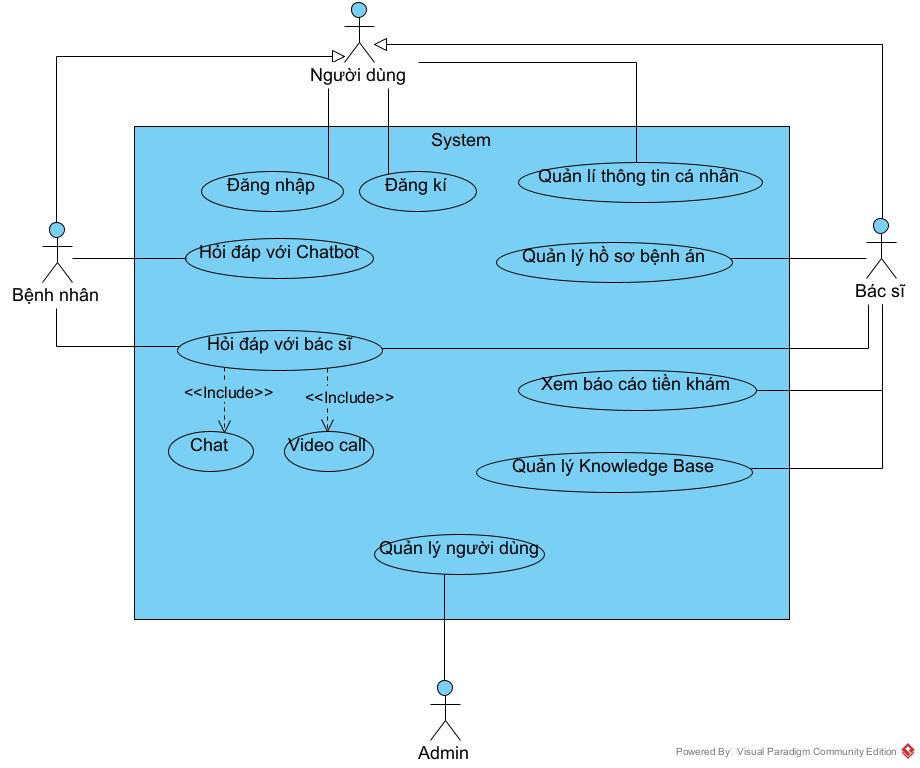
\includegraphics[width=0.95\linewidth,height=0.7\textheight,keepaspectratio]{chuong2/hinh/usecase_tong_quan.jpg}
  \caption{Sơ đồ use case tổng quan của hệ thống}
  \label{fig:usecase_tong_quan}
\end{figure}

Hệ thống được chia thành các nhóm chức năng chính bao gồm:
\begin{itemize}
  \item \textbf{Usecase Đăng ký (Sign Up):} Cho phép người dùng mới tạo tài khoản trên hệ thống với vai trò tương ứng (bệnh nhân hoặc bác sĩ).
  \item \textbf{Usecase Đăng nhập (Sign In):} Xác thực danh tính người dùng (sử dụng JWT token) để truy cập vào các chức năng tương ứng với quyền hạn của mình.
  \item \textbf{Usecase Quản lý thông tin cá nhân (Profile Management):} Cho phép xem, cập nhật và chỉnh sửa thông tin cá nhân, liên hệ, chuyên môn (đối với bác sĩ) hoặc quản lý nhiều hồ sơ y tế thành viên trong gia đình (đối với bệnh nhân).
  \item \textbf{Usecase Quản lý người dùng (User Administration):} Dành cho quản trị viên nhằm kiểm tra, phê duyệt hồ sơ bác sĩ và kiểm soát trạng thái hoạt động của các tài khoản.
\end{itemize}

\subsection{Use case chi tiết}

Phần này trình bày kịch bản chuẩn và các ngoại lệ cho từng use case chính của hệ thống theo mẫu use case chi tiết (use case, tác nhân, tiền/hậu điều kiện, kịch bản chính và ngoại lệ). Biểu đồ use case chi tiết cho từng use case được bổ sung riêng. Trong các kịch bản, hệ thống được gọi chung là ``hệ thống''; các giá trị cụ thể (tên đăng nhập, mật khẩu, dữ liệu mẫu) lấy từ tài khoản demo.

\subsubsection{UC1: Đăng ký và đăng nhập}

\begin{figure}[H]
  \centering
  
\includegraphics[width=0.4\linewidth,keepaspectratio]{chuong2/hinh/dang_nhap.jpg}
  \caption{Sơ đồ use case chi tiết -- UC1: Đăng ký và đăng nhập}
  \label{fig:uc1}
\end{figure}

Chức năng đăng nhập/đăng ký có các giao diện tương tác với người dùng:

\begin{itemize}[nosep,leftmargin=*]
  \item Đăng nhập/đăng ký -> Đề xuất UC đăng nhập/đăng ký
\end{itemize}

Như vậy, biểu đồ UC chi tiết cho modul đăng nhập/đăng ký được trình bày trong Hình trên. Các UC được mô tả như sau:

\begin{itemize}[nosep,leftmargin=*]
  \item \textbf{Đăng nhập/đăng ký}: UC này cho phép người dùng thực hiện đăng nhập hoặc đăng ký tài khoản để truy cập vào hệ thống.
\end{itemize}

% bảng use case giãn dòng như văn bản: tắt giãn dòng đơn mặc định của longtable
\renewcommand{\tablespacing}{}
\begin{spacing}{1.5}
\renewcommand{\arraystretch}{1.15}
\begin{longtable}{|>{\raggedright\arraybackslash}p{0.18\textwidth}|>{\raggedright\arraybackslash}p{0.77\textwidth}|}
\hline
\textbf{Use case} & Đăng ký / Đăng nhập \\ \hline
\textbf{Tác nhân} & Người dùng (Bệnh nhân, Bác sĩ, Quản trị viên) \\ \hline
\textbf{Tiền điều kiện} & Chưa đăng nhập vào hệ thống. \\ \hline
\textbf{Hậu điều kiện} & Người dùng được xác thực, nhận cặp token (Access Token, Refresh Token) và chuyển vào giao diện tương ứng với vai trò. \\ \hline
\textbf{Kịch bản chính} &
\begin{enumerate}[nosep,leftmargin=*]
  \item Người dùng mở ứng dụng, giao diện đăng nhập hiện lên với hai ô ``Tên đăng nhập'' và ``Mật khẩu'' cùng nút ``Đăng nhập''.
  \item Nhập tên đăng nhập = \texttt{user-1}, mật khẩu = \texttt{123456}, nhấn ``Đăng nhập''; hệ thống kiểm tra tên đăng nhập tồn tại và so khớp mật khẩu (bcrypt).
  \item Hệ thống phát hành Access Token (JWT, 30 phút) và Refresh Token (30 ngày), lưu Refresh Token trên Redis.
  \item Client lưu token và chuyển vào giao diện theo vai trò.
\end{enumerate} \\ \hline
\textbf{Ngoại lệ} &
\begin{itemize}[nosep,leftmargin=2.6em,labelwidth=2em,labelsep=0.5em,align=left]
  \item[2.] Hệ thống báo đăng nhập không thành công (sai mật khẩu hoặc tài khoản không tồn tại).
  \begin{itemize}[nosep,leftmargin=3em,labelwidth=2.4em,labelsep=0.4em,align=left]
    \item[2.1] Người dùng click ``OK'' của thông báo.
    \item[2.2] Hệ thống hiện giao diện đăng nhập: username = \texttt{user-1}, password = (trống).
    \item[2.3] Người dùng sửa lại mật khẩu thành \texttt{123456}, click ``Đăng nhập''.
    \item[2.4] Giao diện chính của bệnh nhân hiện lên.
  \end{itemize}
  \item[4.] Token hết hạn.
  \begin{itemize}[nosep,leftmargin=3em,labelwidth=2.4em,labelsep=0.4em,align=left]
    \item[4.1] Client dùng Refresh Token để lấy Access Token mới.
    \item[4.2] Nếu Refresh Token hết hạn, hệ thống bắt buộc đăng nhập lại (về bước 1).
  \end{itemize}
\end{itemize} \\ \hline
\end{longtable}
\end{spacing}

\subsubsection{UC2: Hỏi đáp với chatbot tiền chẩn đoán}

\begin{figure}[H]
  \centering
  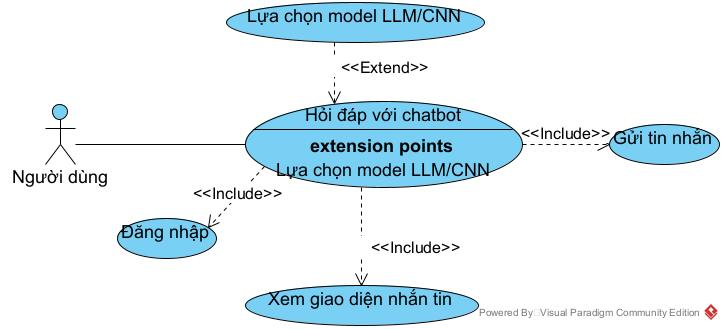
\includegraphics[width=0.95\linewidth,height=0.7\textheight,keepaspectratio]{chuong2/hinh/hoi_dap_chatbot.jpg}
  \caption{Sơ đồ use case chi tiết -- UC2: Hỏi đáp với chatbot tiền chẩn đoán}
  \label{fig:uc2}
\end{figure}

Chức năng hỏi đáp với chatbot tiền chẩn đoán có các giao diện tương tác với người dùng:

\begin{itemize}[nosep,leftmargin=*]
  \item Đăng nhập -> Đề xuất UC đăng nhập
\end{itemize}

\begin{itemize}[nosep,leftmargin=*]
  \item Xem giao diện nhắn tin -> Đề xuất UC xem giao diện nhắn tin
\end{itemize}

\begin{itemize}[nosep,leftmargin=*]
  \item Lựa chọn model LLM/CNN -> Đề xuất UC lựa chọn model LLM/CNN
\end{itemize}

\begin{itemize}[nosep,leftmargin=*]
  \item Gửi tin nhắn -> Đề xuất UC gửi tin nhắn
\end{itemize}

Như vậy, biểu đồ UC chi tiết cho modul hỏi đáp với chatbot tiền chẩn đoán được trình bày trong Hình trên. Các UC được mô tả như sau:

\begin{itemize}[nosep,leftmargin=*]
  \item \textbf{Xem giao diện nhắn tin}: UC này cho phép người dùng xem giao diện trò chuyện chính với chatbot.
\end{itemize}

\begin{itemize}[nosep,leftmargin=*]
  \item \textbf{Lựa chọn model LLM/CNN}: UC này cho phép người dùng tùy chọn mô hình trí tuệ nhân tạo (LLM hoặc CNN) phù hợp để phục vụ cho quá trình hỏi đáp.
\end{itemize}

\begin{itemize}[nosep,leftmargin=*]
  \item \textbf{Gửi tin nhắn}: UC này cho phép người dùng nhập nội dung câu hỏi và gửi đi để nhận phản hồi từ chatbot.
\end{itemize}

\begin{spacing}{1.5}
\renewcommand{\arraystretch}{1.15}
\begin{longtable}{|>{\raggedright\arraybackslash}p{0.18\textwidth}|>{\raggedright\arraybackslash}p{0.77\textwidth}|}
\hline
\textbf{Use case} & Hỏi đáp với chatbot tiền chẩn đoán \\ \hline
\textbf{Tác nhân} & Bệnh nhân, Hệ thống AI \\ \hline
\textbf{Tiền điều kiện} & Bệnh nhân đã đăng nhập và có hồ sơ bệnh nhân. \\ \hline
\textbf{Hậu điều kiện} & Tin nhắn và kết quả tiền chẩn đoán được lưu; các dữ kiện lâm sàng (\textit{clinical facts}) được trích xuất sang hệ thống lâm sàng. \\ \hline
\textbf{Kịch bản chính} &
\begin{enumerate}[nosep,leftmargin=*]
  \item Bệnh nhân mở giao diện chat, chọn model LLM (mặc định Gemma 4 26B) và model CNN (mặc định EfficientNet-B0).
  \item Bệnh nhân nhập mô tả: ``Da mặt nổi nhiều mụn đỏ, ngứa 3 ngày nay'' và đính kèm 1 ảnh tổn thương.
  \item Hệ thống lưu tin nhắn người dùng (kèm \texttt{attached\_files}), tạo tin nhắn assistant (\texttt{status = queued}).
  \item Hệ thống gửi yêu cầu lượt chạy sang tác nhân AI.
  \item Tác nhân AI gọi mô hình CNN để phân loại ảnh, trả về top-5 nhãn kèm \% tin cậy (ví dụ: Acne 82\%, Rosacea 9\%).
  \item Tác nhân AI gọi công cụ tìm kiếm ngữ nghĩa và tra cứu đồ thị tri thức để đối chiếu guideline y khoa.
  \item Tác nhân AI tự động bóc tách các dữ kiện lâm sàng (vị trí: mặt; thời gian: 3 ngày; triệu chứng: ngứa; mức độ: đỏ).
  \item Tác nhân AI stream câu trả lời về giao diện theo thời gian thực (SSE): giải thích tham khảo, khuyến cáo mức độ cấp bách, hướng xử trí.
  \item Kết thúc lượt, hệ thống ghi nhận dữ kiện lâm sàng vào hồ sơ bệnh nhân.
  \item Bệnh nhân xem kết quả tiền chẩn đoán mang tính tham khảo cùng khuyến cáo mức độ cấp bách.
\end{enumerate} \\ \hline
\textbf{Ngoại lệ} &
\begin{itemize}[nosep,leftmargin=2.6em,labelwidth=2em,labelsep=0.5em,align=left]
  \item[5.] Ảnh không tải được từ kho lưu trữ.
  \begin{itemize}[nosep,leftmargin=3em,labelwidth=2.4em,labelsep=0.4em,align=left]
    \item[5.1] Agent báo ``Không tìm thấy ảnh'', tiếp tục xử lý phần văn bản.
    \item[5.2] Hệ thống vẫn stream câu trả lời dựa trên mô tả văn bản.
  \end{itemize}
  \item[8.] LLM hoặc dịch vụ tri thức lỗi.
  \begin{itemize}[nosep,leftmargin=3em,labelwidth=2.4em,labelsep=0.4em,align=left]
    \item[8.1] Agent trả thông báo lỗi, tin nhắn assistant chuyển trạng thái \texttt{done} với nội dung lỗi.
    \item[8.2] Bệnh nhân có thể gửi lại tin nhắn.
  \end{itemize}
\end{itemize} \\ \hline
\end{longtable}
\end{spacing}

\subsubsection{UC3: Đặt lịch hẹn và tiếp nhận lần khám}

\begin{figure}[H]
  \centering
  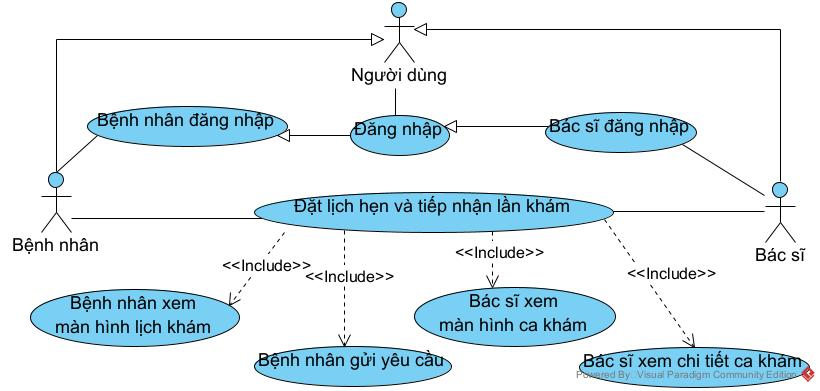
\includegraphics[width=0.95\linewidth,height=0.7\textheight,keepaspectratio]{chuong2/hinh/dat_lich_hen.jpg}
  \caption{Sơ đồ use case chi tiết -- UC3: Đặt lịch hẹn và tiếp nhận lần khám}
  \label{fig:uc3}
\end{figure}

Chức năng đặt lịch hẹn và tiếp nhận lần khám có các giao diện tương tác với bệnh nhân và bác sĩ:

\begin{itemize}[nosep,leftmargin=*]
  \item Đăng nhập (Bệnh nhân đăng nhập, Bác sĩ đăng nhập) -> Đề xuất UC đăng nhập (UC bệnh nhân đăng nhập, UC bác sĩ đăng nhập)
\end{itemize}

\begin{itemize}[nosep,leftmargin=*]
  \item Bệnh nhân xem màn hình lịch khám -> Đề xuất UC bệnh nhân xem màn hình lịch khám
\end{itemize}

\begin{itemize}[nosep,leftmargin=*]
  \item Bệnh nhân gửi yêu cầu -> Đề xuất UC bệnh nhân gửi yêu cầu
\end{itemize}

\begin{itemize}[nosep,leftmargin=*]
  \item Bác sĩ xem màn hình ca khám -> Đề xuất UC bác sĩ xem màn hình ca khám
\end{itemize}

\begin{itemize}[nosep,leftmargin=*]
  \item Bác sĩ xem chi tiết ca khám -> Đề xuất UC bác sĩ xem chi tiết ca khám
\end{itemize}

Như vậy, biểu đồ UC chi tiết cho modul đặt lịch hẹn và tiếp nhận lần khám được trình bày trong Hình trên. Các UC được mô tả như sau:

\begin{itemize}[nosep,leftmargin=*]
  \item \textbf{Bệnh nhân xem màn hình lịch khám}: UC này cho phép bệnh nhân xem thông tin về các lịch khám hiện có trên hệ thống.
\end{itemize}

\begin{itemize}[nosep,leftmargin=*]
  \item \textbf{Bệnh nhân gửi yêu cầu}: UC này cho phép bệnh nhân điền thông tin và gửi yêu cầu đặt lịch hẹn khám bệnh.
\end{itemize}

\begin{itemize}[nosep,leftmargin=*]
  \item \textbf{Bác sĩ xem màn hình ca khám}: UC này cho phép bác sĩ theo dõi danh sách các ca khám được đăng ký.
\end{itemize}

\begin{itemize}[nosep,leftmargin=*]
  \item \textbf{Bác sĩ xem chi tiết ca khám}: UC này cho phép bác sĩ xem thông tin chi tiết của một ca khám cụ thể để thực hiện tiếp nhận lần khám.
\end{itemize}

\begin{spacing}{1.5}
\renewcommand{\arraystretch}{1.15}
\begin{longtable}{|>{\raggedright\arraybackslash}p{0.18\textwidth}|>{\raggedright\arraybackslash}p{0.77\textwidth}|}
\hline
\textbf{Use case} & Đặt lịch hẹn và tiếp nhận lần khám \\ \hline
\textbf{Tác nhân} & Bệnh nhân, Bác sĩ \\ \hline
\textbf{Tiền điều kiện} & Bệnh nhân đã đăng nhập; đợt bệnh của hồ sơ đang mở, chưa quá hạn, đã có giả thuyết của AI và chưa có lịch hẹn còn hiệu lực; bác sĩ đã đăng nhập. \\ \hline
\textbf{Hậu điều kiện} & Lịch hẹn (\texttt{Appointment}) được tạo và được bác sĩ xác nhận; lần khám (\texttt{Encounter}, trạng thái \texttt{open}) được tạo, đợt bệnh chuyển \texttt{in\_exam}, kênh trao đổi bác sĩ -- bệnh nhân được mở. \\ \hline
\textbf{Kịch bản chính} &
\begin{enumerate}[nosep,leftmargin=*]
  \item Bệnh nhân Nguyễn Văn An bấm mục ``Lịch khám'' ở sidebar của giao diện.
  \item Hệ thống hiện màn hình ``Lịch khám'' với 2 tab ``Đang theo dõi'' và ``Lịch hẹn''.
  \item Tab ``Đang theo dõi'' hiện danh sách các vấn đề bệnh nhân đang gặp. Mỗi dòng hiện tên vùng da, thời gian cập nhật, tóm tắt dữ kiện và nút ``Đặt lịch''.
  \item Bệnh nhân bấm ``Đặt lịch'' ở dòng vùng chân (ngứa rát kèm vài mảng đỏ ở cẳng chân).
  \item Hệ thống hiện hộp thoại ``Đặt lịch · Chân'' gồm ô chọn thời gian, ô lý do (không bắt buộc) và nút ``Gửi yêu cầu''.
  \item Bệnh nhân chọn thời gian 08:00 ngày 26/11/2026, nhập lý do rồi bấm ``Gửi yêu cầu''.
\end{enumerate} \\ \cline{2-2}
\textbf{Kịch bản chính (tiếp)} &
\begin{enumerate}[nosep,leftmargin=*,start=7]
  \item Hệ thống kiểm tra điều kiện đặt lịch, tạo lịch hẹn ở trạng thái ``Chờ'', hiện thông báo ``Đã gửi yêu cầu đặt lịch''; dòng vùng chân đổi nút ``Đặt lịch'' thành trạng thái ``Chờ'', tab ``Lịch hẹn'' thêm dòng ``Chân · 26/11/2026 08:00'' kèm dòng phụ ``Chờ bác sĩ nhận'', trạng thái ``Chờ'' và nút ``Huỷ''.
  \item Bác sĩ bấm mục ``Ca khám'' ở sidebar của giao diện.
  \item Hệ thống hiện giao diện ``Ca khám'' gồm bộ lọc trạng thái, ô ``Tìm bệnh nhân'' và bảng các ca khám.
  \item Bác sĩ xem danh sách ca khám, bấm nút ``Xác nhận lịch'' (dấu $\checkmark$) ở dòng của bệnh nhân Nguyễn Văn An.
  \item Hệ thống đổi trạng thái ca khám thành ``Đã hẹn'' và gán bác sĩ cho lịch; phía bệnh nhân, dòng lịch hiện ``BS. Trần Thị Bình'' thay cho ``Chờ bác sĩ nhận''.
  \item Bác sĩ bấm nút ``Bắt đầu khám'' (dấu $\blacktriangleright$): hệ thống đổi trạng thái thành ``Đang khám'' và mở kênh trao đổi bác sĩ -- bệnh nhân.
  \item Hệ thống mở trang ``Chi tiết ca khám'' kèm bản tổng hợp tiền khám: dữ kiện lâm sàng, giả thuyết AI và bằng chứng trích từ chat, ảnh tổn thương kèm dự đoán CNN, lịch sử khám.
  \item Bác sĩ trao đổi thêm với bệnh nhân ở khung ``Trao đổi với bệnh nhân'' và chuẩn bị buổi khám.
\end{enumerate} \\ \hline
\textbf{Ngoại lệ} &
\begin{itemize}[nosep,leftmargin=2.6em,labelwidth=2em,labelsep=0.5em,align=left]
  \item[7.] Không tạo được lịch hẹn: đợt bệnh đã có lịch hẹn còn hiệu lực, chưa đủ thông tin (chưa có giả thuyết AI), đợt bệnh đã quá hạn hoặc thời gian hẹn không ở tương lai.
  \begin{itemize}[nosep,leftmargin=3em,labelwidth=2.4em,labelsep=0.4em,align=left]
    \item[7.1] Hệ thống báo lỗi tương ứng, không tạo lịch hẹn.
    \item[7.2] Bệnh nhân huỷ lịch hẹn cũ (nhập lý do) hoặc quay lại chat mô tả thêm triệu chứng rồi đặt lại với thời gian khác.
  \end{itemize}
  \item[10.] Lịch đã được bác sĩ khác xác nhận trước đó.
  \begin{itemize}[nosep,leftmargin=3em,labelwidth=2.4em,labelsep=0.4em,align=left]
    \item[10.1] Hệ thống báo ``Chỉ xác nhận được lịch hẹn đang chờ.'', lịch đã biến khỏi bộ lọc ``Chờ xác nhận''.
    \item[10.2] Bác sĩ tải lại danh sách ca khám (chỉ bác sĩ đã nhận mới thấy lịch này).
  \end{itemize}
  \item[12.] Không bắt đầu khám được vì đợt bệnh không còn mở.
  \begin{itemize}[nosep,leftmargin=3em,labelwidth=2.4em,labelsep=0.4em,align=left]
    \item[12.1] Hệ thống báo ``Đợt bệnh không còn mở, hãy đổi sang đợt khác hoặc huỷ lịch.''
    \item[12.2] Bác sĩ đổi lịch sang đợt khác của cùng hồ sơ (khối ``Bệnh nhân có vấn đề ở vùng khác\ldots'') hoặc huỷ lịch kèm lý do; nếu bệnh nhân không đến thì đánh dấu ``Bệnh nhân không đến''.
  \end{itemize}
\end{itemize} \\ \hline
\end{longtable}
\end{spacing}

\subsubsection{UC4: Tư vấn trực tiếp và gọi video với bác sĩ}

\begin{figure}[H]
  \centering
  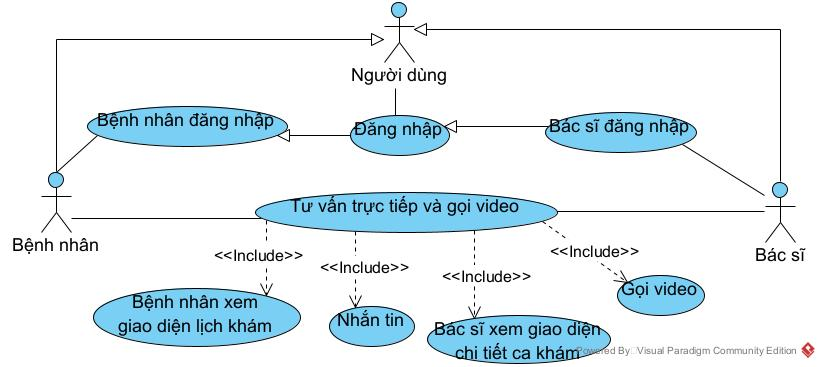
\includegraphics[width=0.95\linewidth,height=0.7\textheight,keepaspectratio]{chuong2/hinh/tu_van_truc_tiep.jpg}
  \caption{Sơ đồ use case chi tiết -- UC4: Tư vấn trực tiếp và gọi video với bác sĩ}
  \label{fig:uc4}
\end{figure}

Chức năng tư vấn trực tiếp và gọi video có các giao diện tương tác với bệnh nhân và bác sĩ:

\begin{itemize}[nosep,leftmargin=*]
  \item Đăng nhập (Bệnh nhân đăng nhập, Bác sĩ đăng nhập) -> Đề xuất UC đăng nhập (UC bệnh nhân đăng nhập, UC bác sĩ đăng nhập)
\end{itemize}

\begin{itemize}[nosep,leftmargin=*]
  \item Bệnh nhân xem giao diện lịch khám -> Đề xuất UC bệnh nhân xem giao diện lịch khám
\end{itemize}

\begin{itemize}[nosep,leftmargin=*]
  \item Bác sĩ xem giao diện chi tiết ca khám -> Đề xuất UC bác sĩ xem giao diện chi tiết ca khám
\end{itemize}

\begin{itemize}[nosep,leftmargin=*]
  \item Nhắn tin -> Đề xuất UC nhắn tin
\end{itemize}

\begin{itemize}[nosep,leftmargin=*]
  \item Gọi video -> Đề xuất UC gọi video
\end{itemize}

Như vậy, biểu đồ UC chi tiết cho modul tư vấn trực tiếp và gọi video được trình bày trong Hình trên. Các UC được mô tả như sau:

\begin{itemize}[nosep,leftmargin=*]
  \item \textbf{Bệnh nhân xem giao diện lịch khám}: UC này cho phép bệnh nhân xem giao diện thông tin lịch khám của mình.
\end{itemize}

\begin{itemize}[nosep,leftmargin=*]
  \item \textbf{Bác sĩ xem giao diện chi tiết ca khám}: UC này cho phép bác sĩ xem giao diện thông tin chi tiết của ca khám cần tư vấn.
\end{itemize}

\begin{itemize}[nosep,leftmargin=*]
  \item \textbf{Nhắn tin}: UC này cho phép bệnh nhân và bác sĩ trao đổi thông tin qua tin nhắn văn bản trực tiếp.
\end{itemize}

\begin{itemize}[nosep,leftmargin=*]
  \item \textbf{Gọi video}: UC này cho phép bệnh nhân và bác sĩ thực hiện cuộc gọi video trực tuyến để phục vụ quá trình thăm khám và tư vấn.
\end{itemize}

\begin{spacing}{1.5}
\renewcommand{\arraystretch}{1.15}
\begin{longtable}{|>{\raggedright\arraybackslash}p{0.18\textwidth}|>{\raggedright\arraybackslash}p{0.77\textwidth}|}
\hline
\textbf{Use case} & Tư vấn trực tiếp và gọi video với bác sĩ \\ \hline
\textbf{Tác nhân} & Bệnh nhân, Bác sĩ \\ \hline
\textbf{Tiền điều kiện} & Đã có cuộc hội thoại hoặc lần khám (\texttt{Encounter}) đang mở. \\ \hline
\textbf{Hậu điều kiện} & Tin nhắn và cuộc gọi video được lưu; bác sĩ quan sát tổn thương trực tiếp. \\ \hline
\textbf{Kịch bản chính} &
\begin{enumerate}[nosep,leftmargin=*]
  \item Bác sĩ và bệnh nhân trao đổi qua kênh chat: bác sĩ gửi ``Bạn có thể gửi ảnh vùng da tổn thương hiện tại không?''.
  \item Bệnh nhân gửi thêm 1 hình ảnh tổn thương qua chat.
  \item Bác sĩ khởi tạo cuộc gọi video (WebRTC); hệ thống tạo \texttt{VideoCall} (trạng thái \texttt{pending}).
  \item Bệnh nhân chấp nhận cuộc gọi; trạng thái chuyển \texttt{ongoing}, bắt đầu ghi nhận thời điểm.
  \item Hai bên trao đổi video thời gian thực: bác sĩ quan sát trực tiếp tổn thương, yêu cầu bệnh nhân xoay camera.
  \item Kết thúc cuộc gọi, trạng thái \texttt{ended}, ghi nhận thời điểm bắt đầu/kết thúc.
\end{enumerate} \\ \hline
\textbf{Ngoại lệ} &
\begin{itemize}[nosep,leftmargin=2.6em,labelwidth=2em,labelsep=0.5em,align=left]
  \item[3.] Kết nối video thất bại (mạng/firewall).
  \begin{itemize}[nosep,leftmargin=3em,labelwidth=2.4em,labelsep=0.4em,align=left]
    \item[3.1] Hệ thống báo lỗi, hai bên tiếp tục trao đổi qua tin nhắn.
    \item[3.2] Bác sĩ có thể thử gọi lại.
  \end{itemize}
  \item[5.] Mất kết nối giữa chừng.
  \begin{itemize}[nosep,leftmargin=3em,labelwidth=2.4em,labelsep=0.4em,align=left]
    \item[5.1] Trạng thái cuộc gọi chuyển \texttt{ended}.
    \item[5.2] Hai bên có thể gọi lại.
  \end{itemize}
\end{itemize} \\ \hline
\end{longtable}
\end{spacing}

\subsubsection{UC5: Chốt báo cáo kết luận và nạp ca bệnh}

\begin{figure}[H]
  \centering
  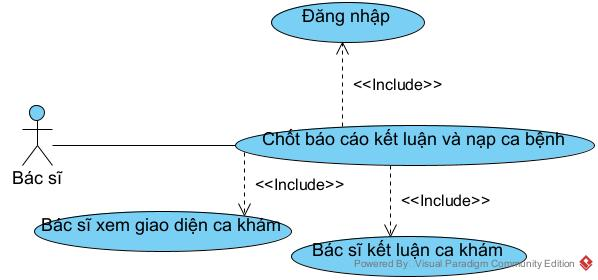
\includegraphics[width=0.95\linewidth,height=0.7\textheight,keepaspectratio]{chuong2/hinh/nap_ca_benh.jpg}
  \caption{Sơ đồ use case chi tiết -- UC5: Chốt báo cáo kết luận và nạp ca bệnh}
  \label{fig:uc5}
\end{figure}

Chức năng chốt báo cáo kết luận và nạp ca bệnh có các giao diện tương tác với bác sĩ:

\begin{itemize}[nosep,leftmargin=*]
  \item Đăng nhập -> Đề xuất UC đăng nhập
\end{itemize}

\begin{itemize}[nosep,leftmargin=*]
  \item Bác sĩ xem giao diện ca khám -> Đề xuất UC bác sĩ xem giao diện ca khám
\end{itemize}

\begin{itemize}[nosep,leftmargin=*]
  \item Bác sĩ kết luận ca khám -> Đề xuất UC bác sĩ kết luận ca khám
\end{itemize}

Như vậy, biểu đồ UC chi tiết cho modul chốt báo cáo kết luận và nạp ca bệnh được trình bày trong Hình trên. Các UC được mô tả như sau:

\begin{itemize}[nosep,leftmargin=*]
  \item \textbf{Bác sĩ xem giao diện ca khám}: UC này cho phép bác sĩ theo dõi và xem thông tin giao diện của các ca khám cần xử lý.
\end{itemize}

\begin{itemize}[nosep,leftmargin=*]
  \item \textbf{Bác sĩ kết luận ca khám}: UC này cho phép bác sĩ nhập thông tin chẩn đoán, chốt báo cáo kết luận cho ca khám và nạp dữ liệu ca bệnh vào hệ thống.
\end{itemize}

\begin{spacing}{1.5}
\renewcommand{\arraystretch}{1.15}
\begin{longtable}{|>{\raggedright\arraybackslash}p{0.18\textwidth}|>{\raggedright\arraybackslash}p{0.77\textwidth}|}
\hline
\textbf{Use case} & Chốt báo cáo kết luận và nạp ca bệnh \\ \hline
\textbf{Tác nhân} & Bác sĩ \\ \hline
\textbf{Tiền điều kiện} & Bác sĩ đã thăm khám (\texttt{Encounter} đang mở). \\ \hline
\textbf{Hậu điều kiện} & Báo cáo kết luận (\texttt{FinalizeReport}) được lưu; ca bệnh được nạp vào Knowledge Base (nếu được chọn làm ca tham khảo). \\ \hline
\textbf{Kịch bản chính} &
\begin{enumerate}[nosep,leftmargin=*]
  \item Bác sĩ nhập nhận định: ``Viêm da cơ địa (Eczema) mức độ trung bình'', hướng điều trị, ghi chú.
  \item Bác sĩ xác nhận các dữ kiện lâm sàng AI đề xuất (ngứa, đỏ, khô da) và điều chỉnh nếu cần.
  \item Hệ thống trích xuất thêm dữ kiện mới từ mô tả bác sĩ.
  \item Hệ thống lưu snapshot báo cáo kết luận (hồ sơ bệnh nhân, mức khẩn cấp, dữ kiện kèm nguồn trích dẫn).
  \item Hệ thống mở kênh theo dõi sau khám (\texttt{doctor\_followup}) với thời hạn 30 ngày.
  \item Bác sĩ đánh dấu ca bệnh tham khảo; hệ thống nạp ca bệnh vào Knowledge Base.
  \item \texttt{Encounter} chuyển trạng thái \texttt{closed}.
\end{enumerate} \\ \hline
\textbf{Ngoại lệ} &
\begin{itemize}[nosep,leftmargin=2.6em,labelwidth=2em,labelsep=0.5em,align=left]
  \item[3.] AI không trích xuất được dữ kiện.
  \begin{itemize}[nosep,leftmargin=3em,labelwidth=2.4em,labelsep=0.4em,align=left]
    \item[3.1] Bác sĩ vẫn chốt báo cáo với dữ kiện đã có.
    \item[3.2] Hệ thống lưu báo cáo bình thường.
  \end{itemize}
  \item[4.] Thiếu chẩn đoán khi đã có \texttt{Encounter}.
  \begin{itemize}[nosep,leftmargin=3em,labelwidth=2.4em,labelsep=0.4em,align=left]
    \item[4.1] Hệ thống báo lỗi.
    \item[4.2] Bác sĩ bổ sung chẩn đoán, hệ thống lưu báo cáo.
  \end{itemize}
\end{itemize} \\ \hline
\end{longtable}
\end{spacing}

\subsubsection{UC6: Số hóa giáo trình vào Knowledge Base}

\begin{figure}[H]
  \centering
  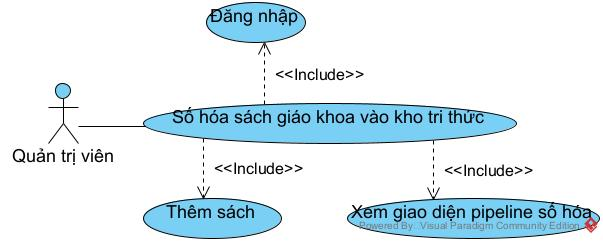
\includegraphics[width=0.95\linewidth,height=0.7\textheight,keepaspectratio]{chuong2/hinh/nap_kb.jpg}
  \caption{Sơ đồ use case chi tiết -- UC6: Số hóa giáo trình vào Knowledge Base}
  \label{fig:uc6}
\end{figure}

Chức năng số hóa sách giáo khoa vào kho tri thức có các giao diện tương tác với quản trị viên:

\begin{itemize}[nosep,leftmargin=*]
  \item Đăng nhập -> Đề xuất UC đăng nhập
\end{itemize}

\begin{itemize}[nosep,leftmargin=*]
  \item Thêm sách -> Đề xuất UC thêm sách
\end{itemize}

\begin{itemize}[nosep,leftmargin=*]
  \item Xem giao diện pipeline số hóa -> Đề xuất UC xem giao diện pipeline số hóa
\end{itemize}

Như vậy, biểu đồ UC chi tiết cho modul số hóa sách giáo khoa vào kho tri thức được trình bày trong Hình trên. Các UC được mô tả như sau:

\begin{itemize}[nosep,leftmargin=*]
  \item \textbf{Thêm sách}: UC này cho phép quản trị viên tải lên và thêm các tài liệu sách giáo khoa mới vào hệ thống để tiến hành xử lý.
\end{itemize}

\begin{itemize}[nosep,leftmargin=*]
  \item \textbf{Xem giao diện pipeline số hóa}: UC này cho phép quản trị viên theo dõi tiến trình và giao diện luồng xử lý số hóa dữ liệu sách giáo khoa vào kho tri thức.
\end{itemize}

\begin{spacing}{1.5}
\renewcommand{\arraystretch}{1.15}
\begin{longtable}{|>{\raggedright\arraybackslash}p{0.18\textwidth}|>{\raggedright\arraybackslash}p{0.77\textwidth}|}
\hline
\textbf{Use case} & Số hóa giáo trình vào Knowledge Base \\ \hline
\textbf{Tác nhân} & Quản trị viên, Knowledge Worker \\ \hline
\textbf{Tiền điều kiện} & Quản trị viên đã đăng nhập; có file PDF giáo trình. \\ \hline
\textbf{Hậu điều kiện} & Tài liệu được trích xuất, phân đoạn và nạp vector vào Qdrant; có thể truy xuất qua RAG. \\ \hline
\textbf{Kịch bản chính} &
\begin{enumerate}[nosep,leftmargin=*]
  \item Quản trị viên tải lên file PDF giáo trình da liễu (ví dụ ``Habif Clinical Dermatology.pdf'', 45 MB).
  \item Hệ thống kiểm tra file PDF hợp lệ (bắt đầu bằng \texttt{\%PDF}, kích thước $\le$ 500 MB), tạo bản ghi \texttt{Document} và 4 bước (\texttt{ingest}, \texttt{toc}, \texttt{chunks}, \texttt{index}) ở trạng thái \texttt{not\_started}.
  \item Knowledge Worker thực thi bước \textit{ingest}: trích xuất văn bản từng trang, lưu \texttt{pages.jsonl} vào MinIO.
  \item Người duyệt xem kết quả, nhấn \texttt{approve}; bước chuyển \texttt{approved}.
  \item Knowledge Worker thực thi bước \textit{toc}: AI nhận diện cấu trúc mục lục, trả về cây mục; người duyệt chỉnh sửa (\textit{override}) nếu cần, rồi \texttt{approve}.
  \item Knowledge Worker thực thi bước \textit{chunks}: phân đoạn văn bản theo mục lục, lưu \texttt{chunks.jsonl}.
  \item Knowledge Worker thực thi bước \textit{index}: sinh vector nhúng (OpenRouter) và nạp vào Qdrant.
  \item Tài liệu sẵn sàng phục vụ truy xuất ngữ nghĩa cho tác nhân AI.
\end{enumerate} \\ \hline
\textbf{Ngoại lệ} &
\begin{itemize}[nosep,leftmargin=2.6em,labelwidth=2em,labelsep=0.5em,align=left]
  \item[2.] File không phải PDF hoặc vượt 500 MB.
  \begin{itemize}[nosep,leftmargin=3em,labelwidth=2.4em,labelsep=0.4em,align=left]
    \item[2.1] Hệ thống từ chối upload, báo lỗi.
    \item[2.2] Người dùng chọn file khác và tải lại.
  \end{itemize}
  \item[3.] Một bước thất bại.
  \begin{itemize}[nosep,leftmargin=3em,labelwidth=2.4em,labelsep=0.4em,align=left]
    \item[3.1] Trạng thái \texttt{failed}, thông báo lỗi hiển thị nguyên văn.
    \item[3.2] Người duyệt sửa tham số và chạy lại.
  \end{itemize}
\end{itemize} \\ \hline
\end{longtable}
\end{spacing}
\renewcommand{\tablespacing}{\singlespacing}
\section{Thiết kế thực thể}

\subsection{Các lớp thực thể liên quan}

Để hiện thực hóa các yêu cầu nghiệp vụ của hệ thống, sơ đồ lớp tổng thể được thiết kế nhằm mô hình hóa đầy đủ các đối tượng thực thể và mối liên kết giữa chúng. Sơ đồ lớp tổng quan của hệ thống được biểu diễn trong Hình~\ref{fig:so_do_lop}.

\begin{sidewaysfigure}[p]
  \centering
  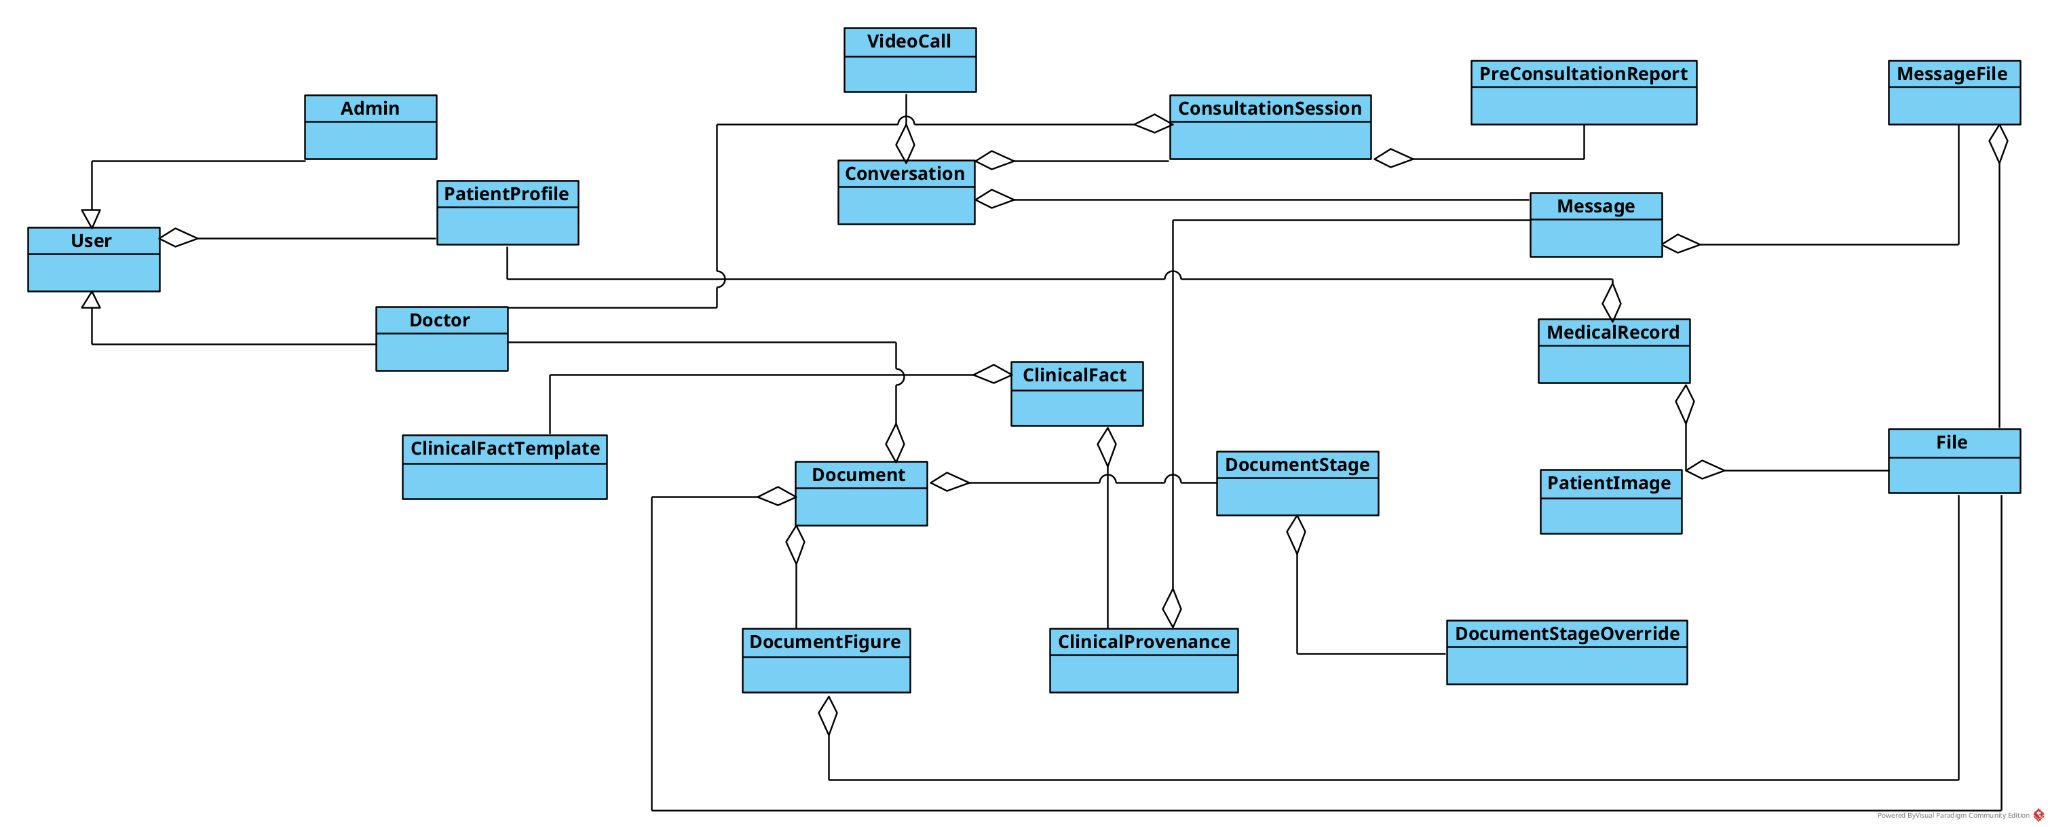
\includegraphics[width=0.95\linewidth]{chuong2/hinh/so_do_lop.png}
  \caption{Sơ đồ lớp thực thể của hệ thống}
  \label{fig:so_do_lop}
\end{sidewaysfigure}

Các lớp thực thể chính trong hệ thống được phân chia thành các nhóm miền nghiệp vụ rõ rệt:
\begin{itemize}
  \item \textbf{Nhóm Người dùng và Hồ sơ (\texttt{User}, \texttt{PatientProfile}, \texttt{Doctor}, \texttt{Admin}):} Quản lý tài khoản đăng nhập, thông tin chuyên môn của bác sĩ, và cho phép một tài khoản quản lý nhiều hồ sơ bệnh nhân (bản thân và các thành viên trong gia đình).
  \item \textbf{Nhóm Hội thoại và Tương tác (\texttt{Conversation}, \texttt{Message}, \texttt{MessageFile}, \texttt{VideoCall}):} Lưu trữ các phiên trao đổi tin nhắn giữa bệnh nhân, trợ lý AI và bác sĩ; ghi nhận các tập tin đính kèm và thông tin phiên gọi video trực tuyến.
  \item \textbf{Nhóm Lâm sàng và Bệnh án (\texttt{Episode}, \texttt{Appointment}, \texttt{Encounter}, \texttt{ClinicalFact}, \texttt{ClinicalProvenance}, \texttt{FinalizeReport}, \texttt{PatientImage}):} Quản lý đợt tiến triển bệnh (\textit{Episode}), lịch hẹn và lần khám, lưu vết nguồn gốc dữ kiện trích xuất từ tin nhắn (\textit{Provenance}), cùng báo cáo kết luận chẩn đoán và hình ảnh y khoa đã được bác sĩ xác nhận.
  \item \textbf{Nhóm Kho tri thức và Tài liệu (\texttt{Document}, \texttt{DocumentStage}, \texttt{DocumentOverride}, \texttt{File}):} Quản lý siêu dữ liệu tập tin lưu trữ trên MinIO, thông tin sách giáo trình y khoa, tiến trình thực thi qua từng bước của pipeline số hóa và các bản ghi can thiệp thủ công từ chuyên gia.
\end{itemize}

\subsection{Quan hệ giữa các lớp thực thể}

Mối quan hệ giữa các lớp thực thể trong hệ thống phản ánh chặt chẽ quy trình nghiệp vụ khám chữa bệnh và bảo đảm tính toàn vẹn dữ liệu:

\begin{itemize}
  \item \textbf{Quan hệ \texttt{User} -- \texttt{PatientProfile} (1--$n$):} Một tài khoản người dùng có thể tạo và quản lý nhiều hồ sơ bệnh nhân khác nhau. Mọi tương tác hội thoại, lịch hẹn và bệnh án lâm sàng đều liên kết trực tiếp với mã định danh \dbname{patient\_profile\_id} thay vì tài khoản \texttt{User}, giúp tách bạch lịch sử bệnh lý của từng cá nhân.
  \item \textbf{Quan hệ \texttt{Appointment} -- \texttt{Encounter} (1--1):} Bệnh nhân đặt lịch hẹn khám (\texttt{Appointment}) với một bác sĩ cụ thể. Khi bác sĩ tiếp nhận, một lần khám (\texttt{Encounter}) được khởi tạo để theo dõi tiến trình thăm khám thực tế. Mỗi lịch hẹn chỉ sinh ra một lần khám.
  \item \textbf{Quan hệ \texttt{Episode} -- \texttt{ClinicalFact} (1--$n$):} Một đợt bệnh biểu diễn một giai đoạn tổn thương da cụ thể, chứa nhiều dữ kiện lâm sàng (\texttt{ClinicalFact}). Dữ kiện dài hạn như tiền sử dị ứng, thuốc đang dùng được gắn với hồ sơ bệnh nhân và không thuộc đợt bệnh nào.
  \item \textbf{Quan hệ \texttt{ClinicalFact} -- \texttt{ClinicalProvenance} (1--$n$):} Mỗi dữ kiện lâm sàng có thể được ghi nhận từ nhiều nguồn khác nhau. Mỗi dòng lưu vết ghi lại một lần một nguồn (\texttt{chat}, \texttt{doctor}, \texttt{profile}) xác lập giá trị của dữ kiện, kèm trích dẫn nguyên văn và thời điểm ghi nhận.
  \item \textbf{Quan hệ \texttt{Message} -- \texttt{ClinicalProvenance} ($n$--1):} Mỗi dòng lưu vết trỏ tới tối đa một tin nhắn nguồn ở dịch vụ tư vấn, lưu dưới dạng id mềm và không ràng buộc khoá ngoại. Nhờ đó bác sĩ truy vết được dữ kiện do chatbot trích xuất về đúng tin nhắn và hình ảnh mà bệnh nhân đã gửi, phục vụ đối soát và kiểm chứng lâm sàng.
  \item \textbf{Quan hệ \texttt{Encounter} -- \texttt{FinalizeReport} (1--1):} Khi kết thúc lần khám, bác sĩ chốt báo cáo kết luận (\texttt{FinalizeReport}) gắn với \texttt{Encounter}. Báo cáo này lưu giữ snapshot toàn bộ nhận định chẩn đoán và dữ kiện lâm sàng đã được bác sĩ xác nhận. Nếu được đánh dấu là ca tham khảo chuẩn (\dbname{is\_reference\_case}), dữ liệu sẽ được ẩn danh và nạp sang kho tri thức vector (Qdrant) và đồ thị PJKG để phục vụ các ca tương tự sau này.
  \item \textbf{Quan hệ \texttt{Document} -- \texttt{DocumentStage} (1--$n$):} Một tài liệu giáo trình (\texttt{Document}) sở hữu nhiều bước xử lý (\texttt{DocumentStage}). Cặp \dbname{document\_id} và \dbname{stage\_id} là duy nhất, nên mỗi bước chỉ có một bản ghi trạng thái trên một tài liệu.
  \item \textbf{Quan hệ \texttt{DocumentStage} -- \texttt{DocumentOverride} (1--1):} Mỗi bước có tối đa một bản ghi \texttt{DocumentOverride} lưu các can thiệp chỉnh sửa tay của chuyên gia; khoá chính của bảng chính là \dbname{document\_stage\_id}. Nhờ vậy chạy lại máy không làm mất công sức hiệu đính của người duyệt.
\end{itemize}

\section{Thiết kế kiến trúc microservice}

\subsection{Phân rã service}

\subsubsection{Nguyên tắc phân rã}
Hệ thống được phân rã dựa trên nguyên lý thiết kế hướng miền (Domain-Driven Design - DDD). Mỗi dịch vụ chịu trách nhiệm cho một miền nghiệp vụ độc lập, sở hữu cơ sở dữ liệu riêng biệt (Database-per-Service) nhằm đảm bảo tính độc lập về triển khai, bảo trì và khả năng mở rộng quy mô linh hoạt theo nhu cầu tải.

\subsubsection{Danh sách service theo domain}
Dựa trên phân tích nghiệp vụ khám chữa bệnh da liễu và các tác vụ trí tuệ nhân tạo, hệ thống được phân chia thành 6 dịch vụ chính:
\begin{itemize}
  \item \dbname{gateway\_service}: API Gateway, quản lý định tuyến lưu lượng và reverse proxy.
  \item \dbname{identity\_service}: Quản lý tài khoản, phân quyền và hồ sơ bệnh nhân.
  \item \dbname{consultation\_service}: Quản lý phiên hội thoại, tin nhắn và kênh theo dõi sau khám.
  \item \dbname{clinical\_service}: Quản lý hồ sơ bệnh án, lịch hẹn, đợt bệnh và báo cáo kết luận.
  \item \dbname{knowledge\_service}: Quản lý pipeline số hóa sách, vector database và đồ thị tri thức.
  \item \dbname{ai\_service}: Quản lý tác nhân lập luận LangGraph, mô hình CNN và xử lý dữ kiện lâm sàng.
\end{itemize}

Mỗi dịch vụ sở hữu một lược đồ cơ sở dữ liệu riêng, không dùng chung bảng. Sơ đồ cơ sở dữ liệu của bốn dịch vụ có lưu trữ quan hệ được thể hiện trong Hình~\ref{fig:services_db}.

\begin{sidewaysfigure}[p]
  \centering
  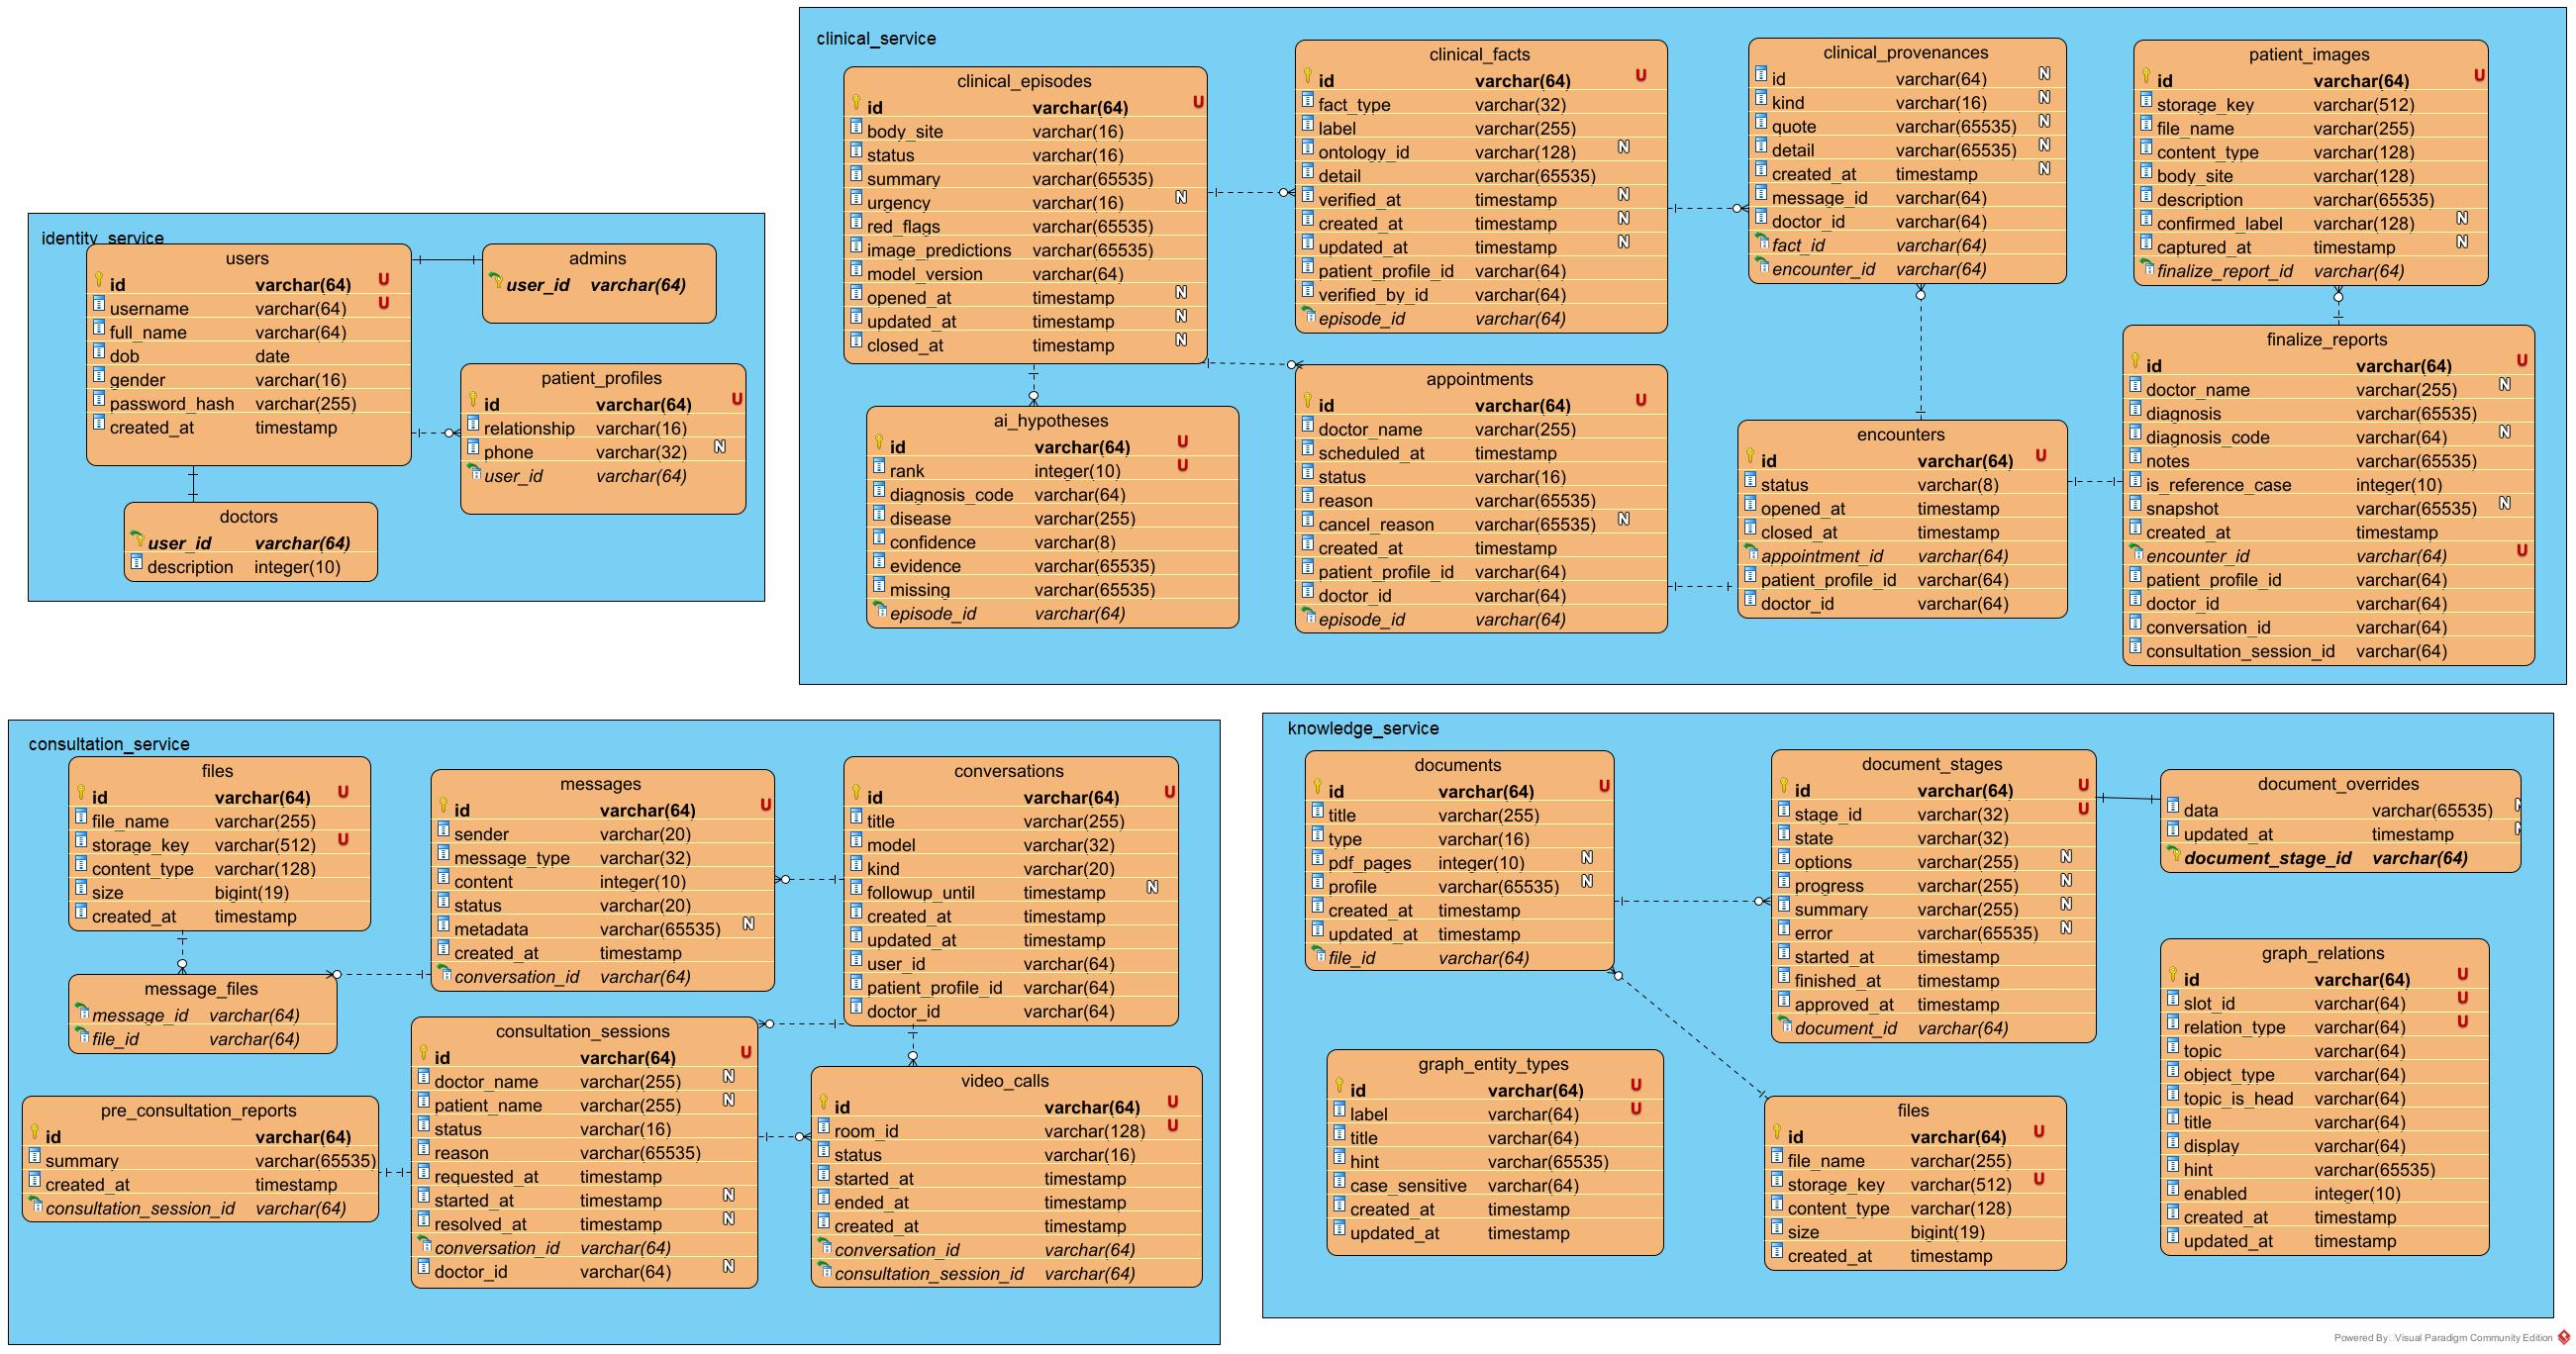
\includegraphics[width=0.95\linewidth]{chuong2/hinh/services_db.jpg}
  \caption{Sơ đồ cơ sở dữ liệu theo từng dịch vụ trong kiến trúc microservice}
  \label{fig:services_db}
\end{sidewaysfigure}
\clearpage

\subsubsection{Kiến trúc tổng thể (Client, API Gateway, Server, Database)}
Kiến trúc tổng thể của hệ thống gồm tầng Client (giao diện Next.js cho Bệnh nhân, Bác sĩ và Quản trị viên), tầng cổng kết nối API Gateway tiếp nhận các yêu cầu REST/SSE, tầng dịch vụ nghiệp vụ (Spring Boot và Python FastAPI/LangGraph) cùng tầng lưu trữ dữ liệu đa mô hình gồm PostgreSQL, Redis, MinIO, Qdrant và Neo4j. Bốn tầng này được thể hiện trong Hình~\ref{fig:kien_truc_tong_the}.

\begin{figure}[H]
  \centering
  \begin{singlespace}
  \begin{tikzpicture}[
    font=\scriptsize,
    >=Stealth,
    tierbox/.style={rounded corners=2pt, align=center, inner sep=2pt, line width=1.3pt},
    svc/.style={draw=teal!90!black, fill=teal!4, rounded corners=2pt, align=center,
      minimum width=3.0cm, minimum height=0.8cm, inner sep=2pt, line width=1.1pt},
    data/.style={draw=green!50!black, fill=green!7, rounded corners=2pt, align=center,
      minimum height=1.6cm, inner sep=1pt, line width=1.1pt},
    infra/.style={draw=black!60, fill=black!5, rounded corners=2pt, align=center,
      minimum height=1.6cm, inner sep=1pt, line width=1pt},
    frame/.style={draw=black!60, fill=black!3, rounded corners=3pt, line width=0.9pt},
    link/.style={->, draw=black!85, line width=0.8pt},
    external/.style={draw=black!70, dashed, fill=black!3, rounded corners=2pt, align=center,
      inner sep=2pt, line width=1pt},
    note/.style={font=\scriptsize, text=black!80, align=center}
  ]

  % ---------- tầng client ----------
  \node[tierbox, draw=blue!75!black, fill=blue!4, minimum width=6.0cm, minimum height=0.8cm] (client) at (8.0,14.5)
    {\textbf{Next.js}};

  % ---------- tầng gateway ----------
  \node[tierbox, draw=red!70!black, fill=red!4, minimum width=15.7cm, minimum height=0.8cm] (gateway) at (8.0,13.15)
    {\textbf{gateway-service} (Spring Cloud Gateway)};

  % ---------- tầng dịch vụ ----------
  \draw[frame] (0.05,11.0) rectangle (15.95,12.4);

  \node[svc] (identity) at (1.7,11.7) {\textbf{identity-service}};
  \node[svc] (consultation) at (4.85,11.7) {\textbf{consultation-service}};
  \node[svc] (clinical) at (8.0,11.7) {\textbf{clinical-service}};
  \node[svc] (knowledge) at (11.15,11.7) {\textbf{knowledge-service}};
  \node[svc] (ai) at (14.3,11.7) {\textbf{ai-service}};

  % ---------- mô hình ngôn ngữ ngoài hệ thống ----------
  \node[external, minimum width=3.2cm, minimum height=0.8cm] (llm) at (14.3,10.05)
    {\textbf{LLM}\\\\{\scriptsize OpenRouter · Ollama}};

  % ---------- tầng dữ liệu ----------
  \draw[frame] (0.05,6.3) rectangle (15.95,9.05);
  \node[note, anchor=west] at (0.3,8.82) {mỗi dịch vụ sở hữu một database riêng};

  \node[data, minimum width=3.8cm] (postgres) at (2.3,7.5)
    {\textbf{PostgreSQL}\\{\scriptsize identity · consultation}\\{\scriptsize clinical · knowledge}\\{\scriptsize ai (checkpoint)}};
  \node[infra, minimum width=2.1cm] (redis) at (5.43,7.5)
    {\textbf{Redis}\\{\scriptsize token, stream}};
  \node[infra, minimum width=2.1cm] (minio) at (7.71,7.5)
    {\textbf{MinIO}\\{\scriptsize ảnh, PDF}};
  \node[infra, minimum width=2.1cm] (qdrant) at (9.99,7.5)
    {\textbf{Qdrant}\\{\scriptsize vector}};
  \node[infra, minimum width=2.1cm] (neo4j) at (12.27,7.5)
    {\textbf{Neo4j}\\{\scriptsize đồ thị}};
  \node[infra, minimum width=2.1cm] (rabbit) at (14.55,7.5)
    {\textbf{RabbitMQ}\\{\scriptsize pipeline sách}};

  % ---------- liên kết ----------
  \draw[link] (client.south) -- (gateway.north)
    node[midway, right=3pt, note] {HTTPS: REST \texttt{/api/v1/**}, SSE};
  \foreach \s in {identity, consultation, clinical, knowledge}
    \draw[link] (\s.north|-gateway.south) -- (\s.north);
  \draw[link] (8.0,11.0) -- (8.0,9.05)
    node[midway, left=3pt, note] {SQL · Redis · S3 · vector · graph};
  \draw[link, dashed] (ai.south) -- (llm.north)
    node[pos=0.58, right=3pt, note] {gọi LLM};

\end{tikzpicture}
  \end{singlespace}
  \caption{Kiến trúc tổng thể của hệ thống theo bốn tầng: client, API Gateway, dịch vụ nghiệp vụ và lưu trữ dữ liệu}
  \label{fig:kien_truc_tong_the}
\end{figure}


\subsubsection{Giao tiếp giữa các dịch vụ}
Các dịch vụ nghiệp vụ trao đổi nội bộ thông qua hai cơ chế chính:
\begin{itemize}
  \item \textbf{REST API nội bộ (\texttt{/internal/...}):} Sử dụng giao thức HTTP/1.1 kèm khóa xác thực bí mật chung (\texttt{X-Internal-Key}) để thực hiện các lời gọi đồng bộ giữa các service.
  \item \textbf{Redis Stream:} Sử dụng kênh stream \texttt{conversation:events:\{id\}} để phát và phát lại (replay) các sự kiện xử lý thời gian thực từ Agent đến Client thông qua Server-Sent Events (SSE).
\end{itemize}

\subsection{Thiết kế dịch vụ API Gateway (\dbname{gateway\_service})}

\subsubsection{Chức năng và cơ chế định tuyến}
Dịch vụ API Gateway được xây dựng trên nền tảng Spring Cloud Gateway, đóng vai trò là điểm truy cập duy nhất (Single Point of Entry) cho toàn bộ các ứng dụng Client bên ngoài. Gateway thực hiện định tuyến động các yêu cầu dựa trên tiền tố đường dẫn (Path Prefix) tới các dịch vụ nghiệp vụ tương ứng ở phía sau.

\subsubsection{Cấu hình triển khai}
Gateway lắng nghe tại cổng \texttt{3040}, thiết lập cấu hình CORS tập trung, chuyển tiếp nguyên vẹn các luồng dữ liệu streaming (SSE) và quản lý chuyển tiếp các header xác thực mà không can thiệp sâu vào xử lý nghiệp vụ nội bộ.

\subsection{Thiết kế dịch vụ định danh (\dbname{identity\_service})}

\subsubsection{Chức năng và giao diện lập trình (API)}
Dịch vụ đảm nhận đăng ký, xác thực danh tính người dùng bằng JSON Web Token (JWT), quản lý cơ chế xoay vòng Refresh Token trên Redis, và quản lý hồ sơ thông tin của các bác sĩ cũng như hồ sơ bệnh nhân cá nhân/gia đình.

\subsubsection{Thiết kế cơ sở dữ liệu}
Dịch vụ quản trị cơ sở dữ liệu PostgreSQL độc lập (\dbname{identity\_db}) gồm tài khoản, vai trò và hồ sơ bệnh nhân.
\begin{itemize}
\raggedright
  \item \textbf{Danh sách các bảng:}
  \begin{itemize}
    \item \dbname{users}: \dbname{id} (PK), \dbname{username} (UQ), \dbname{full\_name}, \dbname{dob}, \dbname{gender}, \dbname{password\_hash}, \dbname{created\_at}.
    \item \dbname{doctors}: \dbname{user\_id} \mbox{(PK, FK $\rightarrow$ \dbname{users.id})}, \dbname{description}.
    \item \dbname{admins}: \dbname{user\_id} \mbox{(PK, FK $\rightarrow$ \dbname{users.id})}.
    \item \dbname{patient\_profiles}: \dbname{id} (PK), \dbname{user\_id} \mbox{(FK $\rightarrow$ \dbname{users.id})}, \dbname{full\_name}, \dbname{dob}, \dbname{gender}, \dbname{relationship}, \dbname{phone}, \dbname{created\_at}.
  \end{itemize}
  \item \textbf{Quan hệ giữa các bảng:}
  \begin{itemize}
    \item \dbname{users} -- \dbname{doctors}: Quan hệ 1--1.
    \item \dbname{users} -- \dbname{admins}: Quan hệ 1--1.
    \item \dbname{users} -- \dbname{patient\_profiles}: Quan hệ 1--$n$.
  \end{itemize}
\end{itemize}

\begin{figure}[H]
  \centering
  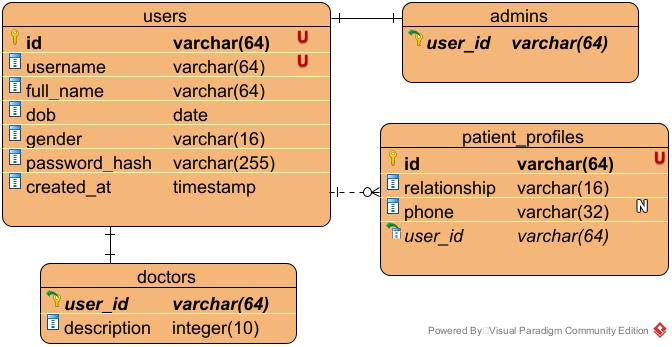
\includegraphics[width=0.95\linewidth,height=0.7\textheight,keepaspectratio]{chuong2/hinh/identity_db.jpg}
  \caption{Sơ đồ cơ sở dữ liệu dịch vụ định danh}
  \label{fig:db_identity}
\end{figure}

\subsection{Thiết kế dịch vụ tư vấn (\dbname{consultation\_service})}

\subsubsection{Chức năng và giao diện lập trình (API)}
Dịch vụ chịu trách nhiệm khởi tạo và lưu trữ các cuộc hội thoại (\texttt{Conversation}), điều phối tin nhắn gửi đến tác nhân AI hoặc bác sĩ, quản lý kênh theo dõi sau khám (\texttt{FollowupChannel}) và xử lý tín hiệu kết nối cho các cuộc gọi video trực tuyến (\texttt{VideoCall}).

\subsubsection{Thiết kế cơ sở dữ liệu}
Dịch vụ sở hữu cơ sở dữ liệu PostgreSQL (\dbname{consultation\_db}) cho hội thoại, tin nhắn, phiên tư vấn và cuộc gọi video; sự kiện thời gian thực đi qua Redis Stream.
\begin{itemize}
\raggedright
  \item \textbf{Danh sách các bảng:}
  \begin{itemize}
    \item \dbname{files}: \dbname{id} (PK), \dbname{file\_name}, \dbname{storage\_key} (UQ), \dbname{content\_type}, \dbname{size}, \dbname{created\_at}.
    \item \dbname{conversations}: \dbname{id} (PK), \dbname{user\_id}, \dbname{patient\_profile\_id}, \dbname{title}, \dbname{model}, \dbname{kind}, \dbname{encounter\_id} (UQ), \dbname{doctor\_id}, \dbname{followup\_until}, \dbname{created\_at}, \dbname{updated\_at}.
    \item \dbname{consultation\_sessions}: \dbname{id} (PK), \dbname{conversation\_id} \mbox{(FK $\rightarrow$ \dbname{conversations.id})}, \dbname{doctor\_id}, \dbname{doctor\_name}, \dbname{patient\_name}, \dbname{status}, \dbname{reason}, \dbname{requested\_at}, \dbname{started\_at}, \dbname{resolved\_at}.
    \item \dbname{messages}: \dbname{id} (PK), \dbname{conversation\_id} \mbox{(FK $\rightarrow$ \dbname{conversations.id})}, \dbname{sender}, \dbname{message\_type}, \dbname{video\_call\_id} \mbox{(FK $\rightarrow$ \dbname{video\_calls.id})}, \dbname{consultation\_session\_id} \mbox{(FK $\rightarrow$ \dbname{consultation\_sessions.id})}, \dbname{content}, \dbname{status}, \dbname{metadata}, \dbname{created\_at}.
    \item \dbname{video\_calls}: \dbname{id} (PK), \dbname{conversation\_id} \mbox{(FK $\rightarrow$ \dbname{conversations.id})}, \dbname{consultation\_session\_id} \mbox{(FK $\rightarrow$ \dbname{consultation\_sessions.id})}, \dbname{room\_id} (UQ), \dbname{status}, \dbname{started\_at}, \dbname{ended\_at}, \dbname{created\_at}.
    \item \dbname{message\_files}: \dbname{message\_id} \mbox{(PK, FK $\rightarrow$ \dbname{messages.id})}, \dbname{file\_id} \mbox{(PK, FK $\rightarrow$ \dbname{files.id})}.
    \item \dbname{pre\_consultation\_reports}: \dbname{id} (PK), \dbname{consultation\_session\_id} \mbox{(UQ, FK $\rightarrow$ \dbname{consultation\_sessions.id})}, \dbname{summary}, \dbname{created\_at}.
  \end{itemize}
  \item \textbf{Quan hệ giữa các bảng:}
  \begin{itemize}
    \item \dbname{conversations} -- \dbname{consultation\_sessions}: Quan hệ 1--$n$.
    \item \dbname{conversations} -- \dbname{messages}: Quan hệ 1--$n$.
    \item \dbname{conversations} -- \dbname{video\_calls}: Quan hệ 1--$n$.
    \item \dbname{consultation\_sessions} -- \dbname{video\_calls}: Quan hệ 1--$n$.
    \item \dbname{consultation\_sessions} -- \dbname{messages}: Quan hệ 1--$n$.
    \item \dbname{consultation\_sessions} -- \dbname{pre\_consultation\_reports}: Quan hệ 1--1.
    \item \dbname{video\_calls} -- \dbname{messages}: Quan hệ 1--$n$.
    \item \dbname{messages} -- \dbname{message\_files}: Quan hệ 1--$n$.
    \item \dbname{files} -- \dbname{message\_files}: Quan hệ 1--$n$.
  \end{itemize}
\end{itemize}

\begin{figure}[H]
  \centering
  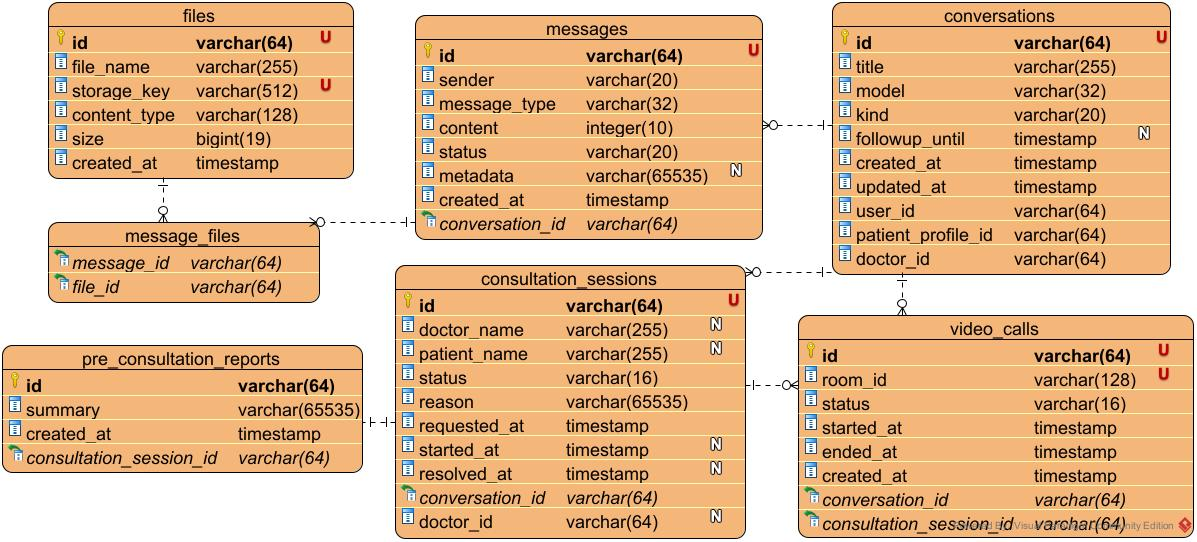
\includegraphics[width=0.95\linewidth,height=0.7\textheight,keepaspectratio]{chuong2/hinh/consultation_db.jpg}
  \caption{Sơ đồ cơ sở dữ liệu dịch vụ tư vấn}
  \label{fig:db_consultation}
\end{figure}

\subsection{Thiết kế dịch vụ lâm sàng (\dbname{clinical\_service})}

\subsubsection{Chức năng và giao diện lập trình (API)}
Dịch vụ quản lý toàn bộ vòng đời bệnh lý của bệnh nhân: lập lịch hẹn khám (\texttt{Appointment}), tiếp nhận lần khám (\texttt{Encounter}), theo dõi đợt bệnh (\texttt{Episode}), lưu trữ các dữ kiện lâm sàng (\texttt{ClinicalFact}) và chốt báo cáo kết luận khám bệnh (\texttt{FinalizeReport}).

\subsubsection{Thiết kế cơ sở dữ liệu}
Dịch vụ quản trị cơ sở dữ liệu \dbname{clinical\_db} cho đợt bệnh, dữ kiện lâm sàng, lịch hẹn, lần khám và báo cáo kết luận.
\begin{itemize}
\raggedright
  \item \textbf{Danh sách các bảng:}
  \begin{itemize}
    \item \dbname{clinical\_episodes}: \dbname{id} (PK), \dbname{patient\_profile\_id}, \dbname{body\_site}, \dbname{status}, \dbname{last\_conversation\_id}, \dbname{summary}, \dbname{summary\_at}, \dbname{urgency}, \dbname{red\_flags}, \dbname{image\_predictions}, \dbname{model\_version}, \dbname{opened\_at}, \dbname{updated\_at}, \dbname{closed\_at}.
    \item \dbname{ai\_hypotheses}: \dbname{id} (PK), \dbname{episode\_id} \mbox{(FK $\rightarrow$ \dbname{clinical\_episodes.id})}, \dbname{rank}, \dbname{diagnosis\_code}, \dbname{disease}, \dbname{confidence}, \dbname{evidence}, \dbname{missing}. UQ (\dbname{episode\_id}, \dbname{rank}).
    \item \dbname{clinical\_facts}: \dbname{id} (PK), \dbname{patient\_profile\_id}, \dbname{episode\_id} \mbox{(FK $\rightarrow$ \dbname{clinical\_episodes.id})}, \dbname{fact\_type}, \dbname{label}, \dbname{ontology\_id}, \dbname{detail}, \dbname{verified\_at}, \dbname{verified\_by\_id}, \dbname{created\_at}, \dbname{updated\_at}.
    \item \dbname{appointments}: \dbname{id} (PK), \dbname{patient\_profile\_id}, \dbname{episode\_id} \mbox{(FK $\rightarrow$ \dbname{clinical\_episodes.id})}, \dbname{doctor\_id}, \dbname{doctor\_name}, \dbname{scheduled\_at}, \dbname{status}, \dbname{reason}, \dbname{cancel\_reason}, \dbname{created\_at}.
    \item \dbname{encounters}: \dbname{id} (PK), \dbname{appointment\_id} \mbox{(UQ, FK $\rightarrow$ \dbname{appointments.id})}, \dbname{patient\_profile\_id}, \dbname{doctor\_id}, \dbname{status}, \dbname{opened\_at}, \dbname{closed\_at}.
    \item \dbname{clinical\_provenances}: \dbname{id} (PK), \dbname{fact\_id} \mbox{(FK $\rightarrow$ \dbname{clinical\_facts.id})}, \dbname{kind}, \dbname{message\_id}, \dbname{quote}, \dbname{doctor\_id}, \dbname{encounter\_id} \mbox{(FK $\rightarrow$ \dbname{encounters.id})}, \dbname{detail}, \dbname{created\_at}.
    \item \dbname{finalize\_reports}: \dbname{id} (PK), \dbname{patient\_profile\_id}, \dbname{doctor\_id}, \dbname{doctor\_name}, \dbname{diagnosis}, \dbname{notes}, \dbname{is\_reference\_case}, \dbname{consultation\_session\_id} (UQ), \dbname{conversation\_id}, \dbname{encounter\_id} \mbox{(UQ, FK $\rightarrow$ \dbname{encounters.id})}, \dbname{diagnosis\_code}, \dbname{snapshot}, \dbname{created\_at}.
    \item \dbname{patient\_images}: \dbname{id} (PK), \dbname{finalize\_report\_id} \mbox{(FK $\rightarrow$ \dbname{finalize\_reports.id})}, \dbname{storage\_key}, \dbname{file\_name}, \dbname{content\_type}, \dbname{body\_site}, \dbname{description}, \dbname{confirmed\_label}, \dbname{captured\_at}.
  \end{itemize}
  \item \textbf{Quan hệ giữa các bảng:}
  \begin{itemize}
    \item \dbname{clinical\_episodes} -- \dbname{ai\_hypotheses}: Quan hệ 1--$n$.
    \item \dbname{clinical\_episodes} -- \dbname{clinical\_facts}: Quan hệ 1--$n$.
    \item \dbname{clinical\_episodes} -- \dbname{appointments}: Quan hệ 1--$n$.
    \item \dbname{appointments} -- \dbname{encounters}: Quan hệ 1--1.
    \item \dbname{clinical\_facts} -- \dbname{clinical\_provenances}: Quan hệ 1--$n$.
    \item \dbname{encounters} -- \dbname{clinical\_provenances}: Quan hệ 1--$n$.
    \item \dbname{encounters} -- \dbname{finalize\_reports}: Quan hệ 1--1.
    \item \dbname{finalize\_reports} -- \dbname{patient\_images}: Quan hệ 1--$n$.
  \end{itemize}
\end{itemize}
Ngoài khoá chính và khoá ngoại, \dbname{clinical\_db} còn dùng ba chỉ mục duy nhất có điều kiện: mỗi vùng cơ thể chỉ có một đợt đang mở, mỗi đợt chỉ có một lịch hẹn còn hiệu lực, và mỗi cặp (phạm vi, loại, nhãn) dữ kiện chỉ có một dòng.

\begin{figure}[H]
  \centering
  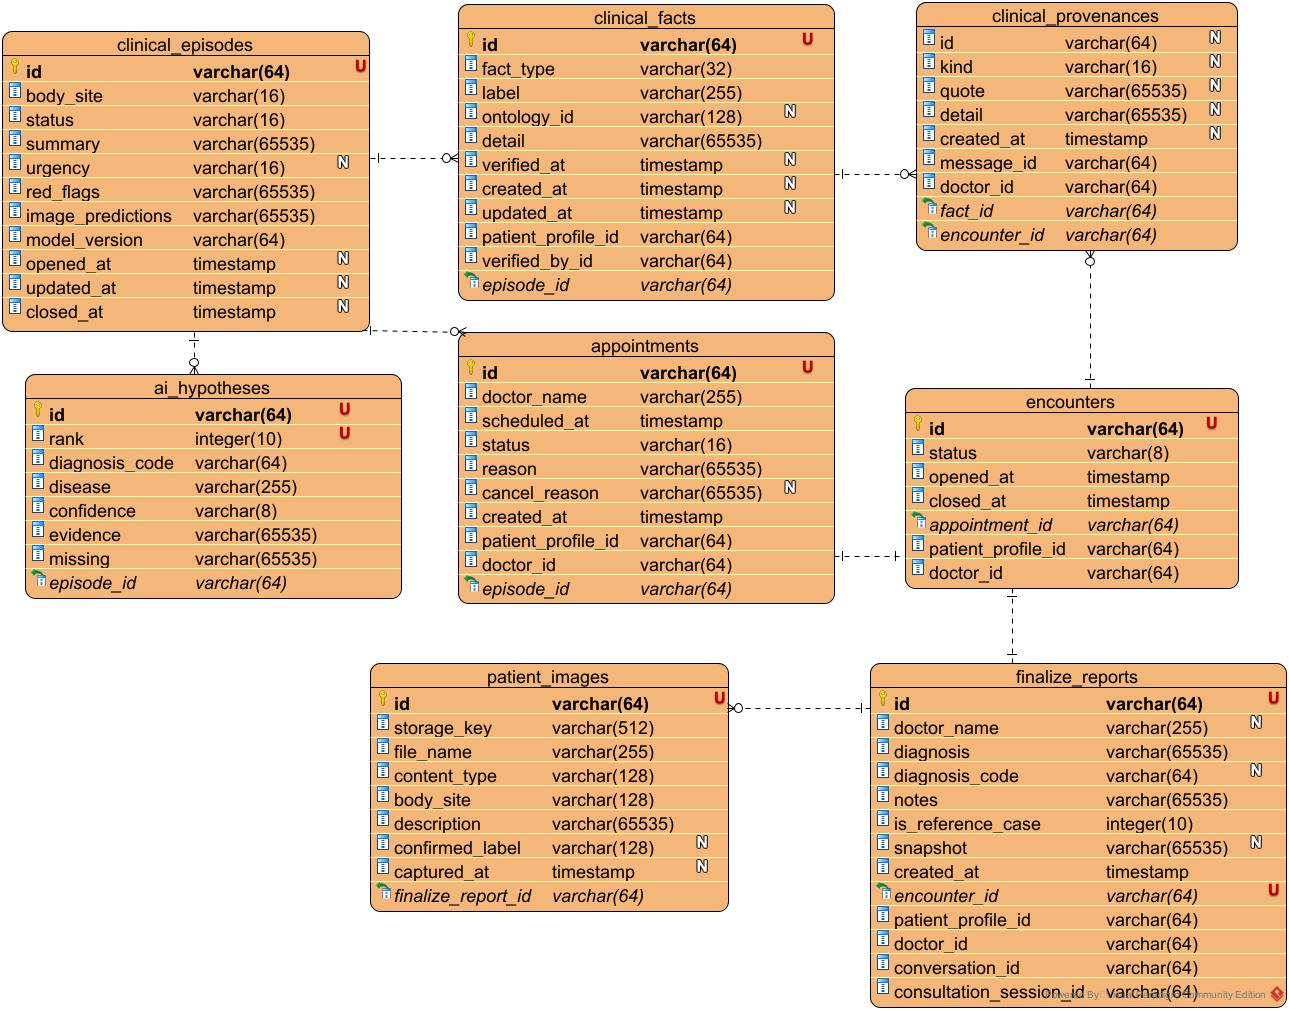
\includegraphics[width=0.95\linewidth,height=0.7\textheight,keepaspectratio]{chuong2/hinh/clinical_db.jpg}
  \caption{Sơ đồ cơ sở dữ liệu dịch vụ lâm sàng}
  \label{fig:db_clinical}
\end{figure}

\subsection{Thiết kế dịch vụ tri thức y khoa (\dbname{knowledge\_service})}

\subsubsection{Chức năng và giao diện lập trình (API)}
Dịch vụ cung cấp các API phục vụ pipeline số hóa tài liệu giáo trình da liễu, tra cứu ngữ nghĩa đa phương thức (Hybrid Search kết hợp Dense Vector và BM25 Sparse), truy vấn đồ thị tri thức bệnh nhân Neo4j và cung cấp URL trích dẫn trang sách y khoa có thể đối soát trực tiếp.

\subsubsection{Thiết kế cơ sở dữ liệu và kho tri thức}
Dịch vụ lưu siêu dữ liệu tài liệu, tiến trình pipeline và danh mục đồ thị trong PostgreSQL (\dbname{knowledge\_db}); nội dung vector ở Qdrant, đồ thị tri thức ở Neo4j, tệp gốc ở MinIO.
\begin{itemize}
\raggedright
  \item \textbf{Danh sách các bảng:}
  \begin{itemize}
    \item \dbname{files}: \dbname{id} (PK), \dbname{file\_name}, \dbname{storage\_key} (UQ), \dbname{content\_type}, \dbname{size}, \dbname{created\_at}.
    \item \dbname{documents}: \dbname{id} (PK), \dbname{title}, \dbname{type}, \dbname{source\_file\_id} \mbox{(FK $\rightarrow$ \dbname{files.id})}, \dbname{ingested\_file\_id} \mbox{(FK $\rightarrow$ \dbname{files.id})}, \dbname{pdf\_pages}, \dbname{uploaded\_by\_id}, \dbname{profile}, \dbname{created\_at}, \dbname{updated\_at}.
    \item \dbname{document\_stages}: \dbname{id} (PK), \dbname{document\_id} \mbox{(FK $\rightarrow$ \dbname{documents.id})}, \dbname{stage\_id}, \dbname{state}, \dbname{options}, \dbname{progress}, \dbname{summary}, \dbname{error}, \dbname{started\_at}, \dbname{finished\_at}, \dbname{approved\_at}. UQ (\dbname{document\_id}, \dbname{stage\_id}).
    \item \dbname{document\_overrides}: \dbname{document\_stage\_id} \mbox{(PK, FK $\rightarrow$ \dbname{document\_stages.id})}, \dbname{data}, \dbname{updated\_at}.
    \item \dbname{graph\_entity\_types}: \dbname{id} (PK), \dbname{label} (UQ), \dbname{title}, \dbname{hint}, \dbname{case\_sensitive}, \dbname{created\_at}, \dbname{updated\_at}.
    \item \dbname{graph\_relations}: \dbname{id} (PK), \dbname{slot\_id} (UQ), \dbname{relation\_type} (UQ), \dbname{topic}, \dbname{object\_type}, \dbname{topic\_is\_head}, \dbname{title}, \dbname{display}, \dbname{hint}, \dbname{entity\_hint}, \dbname{enabled}, \dbname{created\_at}, \dbname{updated\_at}.
  \end{itemize}
  \item \textbf{Quan hệ giữa các bảng:}
  \begin{itemize}
    \item \dbname{files} -- \dbname{documents}: Quan hệ 1--$n$.
    \item \dbname{documents} -- \dbname{document\_stages}: Quan hệ 1--$n$.
    \item \dbname{document\_stages} -- \dbname{document\_overrides}: Quan hệ 1--1.
  \end{itemize}
\end{itemize}

\begin{figure}[H]
  \centering
  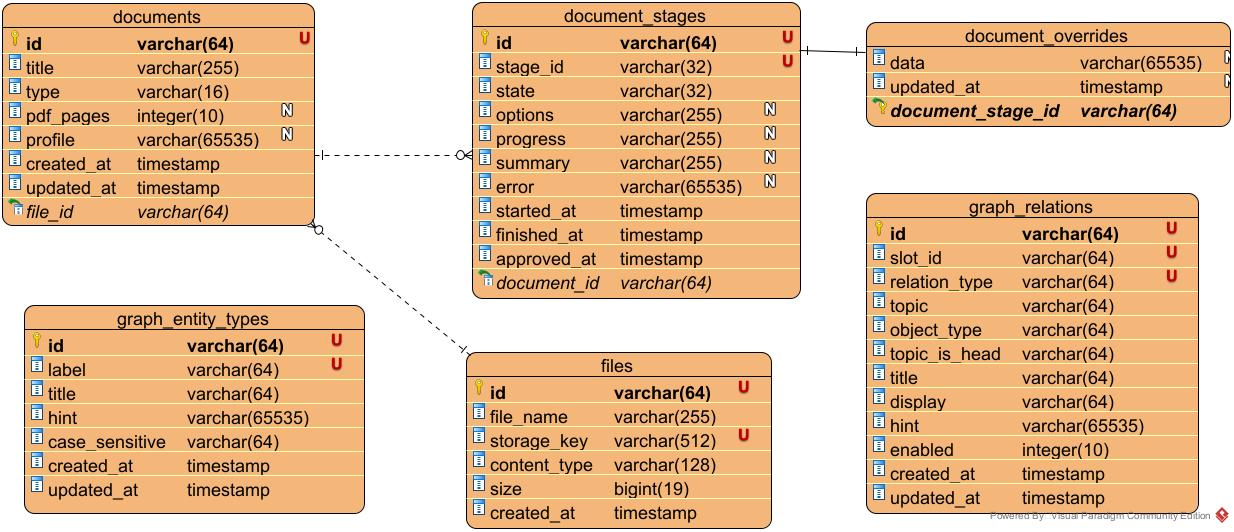
\includegraphics[width=0.95\linewidth,height=0.7\textheight,keepaspectratio]{chuong2/hinh/knowledge_db.jpg}
  \caption{Sơ đồ cơ sở dữ liệu dịch vụ tri thức y khoa}
  \label{fig:db_knowledge}
\end{figure}

\subsection{Thiết kế dịch vụ trí tuệ nhân tạo (\dbname{ai\_service})}

\subsubsection{Chức năng và giao diện lập trình (API)}
Dịch vụ tiếp nhận lượt tương tác qua API nội bộ \texttt{POST /internal/turns}, kích hoạt đồ thị lập luận LangGraph để truy xuất tri thức và sinh lời thoại tư vấn, gọi mô hình phân loại ảnh CNN, và trích xuất tự động các dữ kiện lâm sàng từ mô tả của bác sĩ khi chốt hồ sơ.

\subsubsection{Kiến trúc tác nhân và mô hình AI}
Dịch vụ tích hợp mô hình phân loại đa tổn thương Multi-scale Adaptive CNN với mô hình ngôn ngữ lớn (LLM) theo mô hình tác nhân ReAct có bộ nhớ ngữ cảnh và khả năng tự động gọi công cụ tra cứu tri thức chuyên sâu.

\subsubsection{Thiết kế lưu trữ trạng thái}
Dịch vụ giữ checkpoint của đồ thị lập luận và bộ nhớ dài hạn của tác nhân trong database \texttt{ai}, schema \texttt{langgraph}. Các bảng do thư viện LangGraph tự tạo khi khởi động, không có khoá ngoại sang dữ liệu nghiệp vụ.
\begin{itemize}
\raggedright
  \item \textbf{Danh sách các bảng:}
  \begin{itemize}
    \item \dbname{checkpoints}: \dbname{thread\_id} (PK), \dbname{checkpoint\_ns} (PK), \dbname{checkpoint\_id} (PK), \dbname{parent\_checkpoint\_id}, \dbname{type}, \dbname{checkpoint}, \dbname{metadata}.
    \item \dbname{checkpoint\_blobs}: \dbname{thread\_id} (PK), \dbname{checkpoint\_ns} (PK), \dbname{channel} (PK), \dbname{version} (PK), \dbname{type}, \dbname{blob}.
    \item \dbname{checkpoint\_writes}: \dbname{thread\_id} (PK), \dbname{checkpoint\_ns} (PK), \dbname{checkpoint\_id} (PK), \dbname{task\_id} (PK), \dbname{idx} (PK), \dbname{channel}, \dbname{type}, \dbname{blob}, \dbname{task\_path}.
    \item \dbname{store}: \dbname{prefix} (PK), \dbname{key} (PK), \dbname{value}, \dbname{created\_at}, \dbname{updated\_at}, \dbname{expires\_at}.
    \item \dbname{checkpoint\_migrations}, \dbname{store\_migrations}: phiên bản schema do thư viện quản lý.
  \end{itemize}
  \item \textbf{Quan hệ giữa các bảng:}
  \begin{itemize}
    \item \dbname{checkpoints} -- \dbname{checkpoint\_blobs}: Quan hệ 1--$n$.
    \item \dbname{checkpoints} -- \dbname{checkpoint\_writes}: Quan hệ 1--$n$.
  \end{itemize}
\end{itemize}

\section{Luồng xử lý các chức năng chính}

\subsection{Đăng nhập và đăng ký}

\subsubsection{Mô tả luồng}
Người dùng gửi thông tin đăng ký hoặc đăng nhập thông qua API Gateway. Dịch vụ \dbname{identity\_service} tiến hành xác thực mật khẩu (được mã hóa bằng bcrypt), phát hành cặp token (Access Token và Refresh Token) và trả về cho Client.

\subsubsection{Biểu đồ tuần tự}
Tiến trình tương tác giữa Client, API Gateway và \dbname{identity\_service} trong quá trình xác thực và cấp phát mã định danh được mô hình hóa nhằm đảm bảo an toàn truy cập trên toàn hệ thống.

\subsection{Hỏi đáp với chatbot tiền chẩn đoán}

\subsubsection{Mô tả luồng}
Bệnh nhân gửi tin nhắn kèm hình ảnh tổn thương da. \dbname{consultation\_service} lưu trữ tin nhắn và gửi yêu cầu lượt chạy sang \dbname{ai\_service}. Tác nhân AI gọi mô hình CNN để dự đoán nhãn tổn thương, gọi \dbname{knowledge\_service} để tra cứu tài liệu và stream câu trả lời về cho bệnh nhân qua Redis Stream và SSE. Kết thúc lượt, AI tự động ghi nhận các dữ kiện lâm sàng sang \dbname{clinical\_service}.

\subsubsection{Biểu đồ tuần tự}
Biểu đồ tuần tự minh họa luồng trao đổi bất đồng bộ giữa Client, Gateway, Consultation Service, AI Service, Knowledge Service và Clinical Service trong một lượt tư vấn hoàn chỉnh.

\subsection{Đặt lịch hẹn và tiếp nhận lần khám}

\subsubsection{Mô tả luồng}
Bệnh nhân chọn bác sĩ và thời gian khám trên giao diện để tạo lịch hẹn (\texttt{Appointment}). Bác sĩ kiểm tra danh sách ca và tiếp nhận lần khám (\texttt{Encounter}), hệ thống tự động tải dữ liệu tổng hợp tiền khám từ chatbot để bác sĩ chuẩn bị trước buổi thăm khám.

\subsubsection{Biểu đồ tuần tự}
Mô hình hóa chuỗi tương tác đặt lịch và khởi tạo lần khám giữa bệnh nhân, bác sĩ và dịch vụ lâm sàng.

\subsection{Tư vấn trực tiếp và gọi video với bác sĩ}

\subsubsection{Mô tả luồng}
Trong quá trình khám, bác sĩ và bệnh nhân trao đổi trực tiếp thông qua kênh chat hoặc cuộc gọi video trực tuyến (WebRTC). Bác sĩ có thể yêu cầu bệnh nhân chụp ảnh bổ sung và quan sát trực tiếp tổn thương qua video call.

\subsubsection{Biểu đồ tuần tự}
Biểu đồ tuần tự mô tả quá trình trao đổi tín hiệu (Signaling) và thiết lập kênh truyền dữ liệu video thời gian thực giữa hai phía dưới sự điều phối của \dbname{consultation\_service}.

\subsection{Chốt báo cáo kết luận và nạp ca bệnh}

\subsubsection{Mô tả luồng}
Sau khi thăm khám, bác sĩ nhập nhận định, lý do, mô tả lâm sàng và chọn lọc các dữ kiện AI đề xuất. \dbname{clinical\_service} gọi \dbname{ai\_service} trích xuất dữ kiện mới từ mô tả, lưu snapshot báo cáo kết luận, mở kênh theo dõi sau khám và gửi ca bệnh sang \dbname{knowledge\_service} để nạp vào kho tri thức tham khảo.

\subsubsection{Biểu đồ tuần tự}
Biểu đồ tuần tự mô tả các bước phối hợp giữa Bác sĩ, Clinical Service, AI Service, Consultation Service và Knowledge Service khi hoàn tất một ca khám bệnh.

\subsection{Số hóa giáo trình vào Knowledge Base}

\subsubsection{Mô tả luồng}
Người duyệt tải lên sách giáo khoa PDF. \dbname{knowledge\_service} điều phối Ingest Worker thực thi tuần tự các bước trích xuất nội dung, nhận diện mục lục AI, phân đoạn văn bản và nạp vector vào Qdrant. Người duyệt có thể xem trước và can thiệp sửa đổi kết quả ở từng bước.

\subsubsection{Biểu đồ tuần tự}
Mô hình hóa quá trình phối hợp giữa giao diện quản trị, Knowledge Service, Ingest Worker, LLM và cơ sở dữ liệu vector trong pipeline xử lý tài liệu.

\section{Kết luận}

% Chương 3
\chapter[\MakeUppercase{Kỹ thuật phân loại hình ảnh tổn thương da dựa trên Multi-scale CNN}]{Kỹ thuật phân loại hình ảnh tổn thương da dựa trên Multi-scale CNN}
\label{ch:chuong3}

Chương này trình bày nghiên cứu và xây dựng mô hình thị giác máy tính phục vụ bài toán phân loại tổn thương da từ ảnh chụp lâm sàng. Trước hết, chương phân tích đặc điểm riêng của bài toán phân loại ảnh da liễu và khảo sát các công trình liên quan về kỹ thuật tích chập đa kernel, đa tỷ lệ. Tiếp đó, chương hệ thống hóa cơ sở lý thuyết về mạng nơ-ron tích chập (CNN), kiến trúc ResNet-18 và cơ chế Residual Learning. Trên nền tảng đó, chương trình bày kiến trúc đề xuất AdaptiveCNN --- mô hình kết hợp ResNet-18 với cơ chế tích chập đa kernel thích nghi (AMKC) được đặt trước tầng stem nhằm làm giàu biểu diễn đầu vào ở nhiều phạm vi không gian. Cuối cùng, chương mô tả quy trình huấn luyện, tối ưu mô hình và hệ thống các chỉ số đánh giá định lượng.

% ===================================================================
\section{Bài toán phân loại hình ảnh da liễu}
% ===================================================================

\subsection{Đặc điểm bài toán}

Phân loại ảnh da liễu là bài toán thị giác máy tính nhằm xác định lớp bệnh tương ứng với hình ảnh tổn thương da đầu vào. Với sự phát triển của học sâu, mạng nơ-ron tích chập (Convolutional Neural Network -- CNN) được sử dụng rộng rãi nhờ khả năng tự động học các đặc trưng trực quan từ dữ liệu ảnh, thay vì yêu cầu thiết kế thủ công như phương pháp truyền thống.

Bài toán phân loại ảnh da liễu mang một số thách thức riêng biệt so với phân loại ảnh tự nhiên thông thường:
\begin{itemize}
  \item \textbf{Đa dạng về hình thái tổn thương:} Các tổn thương da khác nhau về kích thước, hình dạng, đường biên và cấu trúc sắc tố. Cùng một bệnh có thể biểu hiện với nhiều hình thái khác nhau (đa hình thái), trong khi các bệnh lý khác nhau lại có thể có biểu hiện trực quan tương tự.
  \item \textbf{Phụ thuộc vào điều kiện chụp ảnh:} Ảnh chụp từ người bệnh trong thực tế có thể khác biệt đáng kể về ánh sáng, góc chụp, độ phân giải và tỷ lệ vùng tổn thương trong khung hình, khác với ảnh soi da chuẩn hóa trong phòng khám.
  \item \textbf{Mất cân bằng phân bố lớp:} Một số bệnh lý phổ biến (như nốt ruồi lành tính) chiếm tỷ lệ áp đảo trong tập dữ liệu, trong khi các bệnh nguy hiểm hơn (như ung thư hắc tố) có số mẫu ít hơn nhiều.
\end{itemize}

Trong phạm vi đồ án, bài toán phân loại tổn thương da được nghiên cứu và đánh giá trên nhiều miền dữ liệu đa dạng: từ ảnh soi da chuyên sâu (Dermoscopy) với 7 nhóm tổn thương (tập HAM10000) và 8 nhóm tổn thương quy mô lớn (tập ISIC 2019), đến ảnh chụp lâm sàng thông thường (Clinical Photography) với 22 lớp bệnh (tập SkinDisease), cũng như ảnh chụp thực tế bằng điện thoại thông minh (Smartphone) với 6 nhóm bệnh (tập PAD-UFES-20). Mô hình thị giác máy tính tiếp nhận ảnh da đầu vào, trích xuất đặc trưng đa tỷ lệ, tổng hợp không gian qua tầng Global Average Pooling và ánh xạ sang phân bố xác suất của các lớp bệnh mục tiêu qua hàm Softmax. Kết quả phân loại này đóng vai trò là một công cụ tính toán (\texttt{predict\_skin\_lesion} tool), cung cấp các giả thuyết bệnh học kèm độ tin cậy định lượng cho tác nhân trí tuệ nhân tạo (LangGraph Agent Worker) kết hợp cùng ngữ cảnh người bệnh và đồ thị tri thức da liễu.

\subsection{Các nghiên cứu liên quan}

Các nghiên cứu về tích chập đa kernel, đặc trưng đa tỷ lệ và tích chập thích nghi cho thấy việc mở rộng cách biểu diễn đặc trưng là một hướng tiếp cận quan trọng trong thị giác máy tính và xử lý ảnh y khoa.

\textbf{Tích chập đa kernel và đa tỷ lệ.} Khan và cộng sự đề xuất MKIS-Net, một mạng nhẹ sử dụng thiết kế multi-kernel để tạo receptive field hiệu quả cho bài toán phân đoạn ảnh y khoa, bao gồm phân đoạn tổn thương da, mạch máu võng mạc và ảnh X-quang ngực. Kết quả cho thấy thiết kế đa kernel có thể hỗ trợ xây dựng mạng gọn nhẹ mà vẫn duy trì hiệu quả cạnh tranh [1]. Han và cộng sự đề xuất DM-CNN cho bài toán phân loại ảnh y khoa, trong đó có dữ liệu da liễu, sử dụng mô-đun Dynamic Multi-scale Feature Fusion để lựa chọn kernel dựa trên đặc trưng ở các tầng khác nhau, kết hợp cơ chế attention và pooling đa tỷ lệ [2].

\textbf{Tích chập thích nghi và lựa chọn kernel.} Hu và cộng sự đề xuất Domain and Content Adaptive Convolution (DCAC) nhằm cải thiện khả năng tổng quát hóa giữa các miền dữ liệu y khoa, điều chỉnh phép tích chập dựa trên thông tin miền và đặc trưng toàn cục của ảnh đầu vào [3]. Chen và cộng sự phát triển ESKNet cho phân đoạn khối u vú trên ảnh siêu âm, trong đó mô-đun Enhanced Selective Kernel Convolution kết hợp biểu diễn từ nhiều vùng đặc trưng và tái hiệu chỉnh thông tin theo chiều kênh lẫn không gian [4].

\textbf{Kết hợp convolution và attention.} AMCANet sử dụng các nhánh convolution attention với những mức lấy mẫu khác nhau nhằm kết hợp thông tin cục bộ và ngữ cảnh không gian cho bài toán khôi phục độ phân giải ảnh [5]. Do nhiệm vụ chính là super-resolution, nghiên cứu này chỉ là tài liệu tham khảo gián tiếp về thiết kế convolution kết hợp attention.

\textbf{Nhận xét và định hướng.} Các nghiên cứu trên thể hiện những hướng tiếp cận khác nhau: thiết kế nhiều kernel, kết hợp đặc trưng đa tỷ lệ, lựa chọn kernel thích nghi và kết hợp convolution với attention. Cần phân biệt ba khái niệm liên quan nhưng không đồng nhất: \textit{multi-kernel} sử dụng nhiều kích thước kernel; \textit{multi-scale} tập trung khai thác đặc trưng ở nhiều phạm vi không gian; còn \textit{adaptive/selective convolution} có thêm cơ chế điều chỉnh hoặc lựa chọn đặc trưng dựa trên đầu vào. Từ cơ sở đó, đồ án sử dụng ResNet-18 làm backbone và tích hợp cơ chế tích chập đa kernel thích nghi (AMKC) trước tầng stem, cho phép mô hình khai thác đặc trưng ở nhiều kích thước ngay từ đầu vào.

% ===================================================================
\section{Cơ sở lý thuyết mạng nơ-ron tích chập}
% ===================================================================

\subsection{Biểu diễn ảnh dưới dạng tensor}

Ảnh màu thường được biểu diễn dưới dạng tensor ba chiều gồm số kênh màu, chiều cao và chiều rộng. Với ảnh RGB có kích thước $H\times W$, tensor ảnh có dạng:
\begin{equation}
  X\in\mathbb{R}^{3\times H\times W}
\end{equation}

Khi xử lý theo lô (batch), dữ liệu có dạng:
\begin{equation}
  X\in\mathbb{R}^{N\times C\times H\times W}
\end{equation}

Trong đó, $N$ là số ảnh trong một batch, $C$ là số kênh, $H$ là chiều cao và $W$ là chiều rộng.

Trước khi đưa vào mạng, ảnh thường được chuyển về kích thước thống nhất ($224\times224$ trong đồ án này) và chuẩn hóa giá trị pixel theo trung bình và độ lệch chuẩn của tập ImageNet. Việc chuẩn hóa giúp dữ liệu có thang giá trị phù hợp với quá trình tối ưu khi sử dụng mô hình pretrained.

\subsection{Phép tích chập}

Phép tích chập (convolution) là thành phần cốt lõi của CNN. Một kernel có kích thước xác định được áp dụng trên các vùng cục bộ của đầu vào để tạo ra feature map. Các trọng số kernel được cập nhật trong quá trình huấn luyện để học những đặc trưng hữu ích cho bài toán.

Dạng tổng quát của phép tích chập hai chiều có thể biểu diễn như sau:
\begin{equation}
  Y_{i,j}=\sum_{c=1}^{C_{\mathrm{in}}}\sum_{u=0}^{K_h-1}\sum_{v=0}^{K_w-1}W_{c,u,v}X_{c,i+u,j+v}+b
\end{equation}

Trong đó, $X$ là tensor đầu vào, $W$ là trọng số kernel, $b$ là bias và $Y$ là feature map đầu ra.

Kích thước kernel quyết định phạm vi không gian được xét trong mỗi phép tính. Kernel $3\times3$ tập trung vào vùng lân cận nhỏ, trong khi kernel $5\times5$ thu nhận thông tin từ vùng rộng hơn. Việc sử dụng nhiều kích thước kernel là cơ sở cho cơ chế AMKC được trình bày ở mục~\ref{sec:amkc}.

\subsection{Hàm kích hoạt và pooling}

Sau phép tích chập, hàm kích hoạt phi tuyến cho phép mạng học những quan hệ phức tạp hơn so với phép biến đổi tuyến tính đơn thuần. Hàm ReLU được sử dụng phổ biến nhất:
\begin{equation}
  \mathrm{ReLU}(x)=\max(0,x)
\end{equation}

Pooling thực hiện giảm kích thước không gian của feature map hoặc tổng hợp thông tin từ các vùng lân cận. Max Pooling lấy giá trị lớn nhất trong mỗi vùng, trong khi Global Average Pooling (GAP) tính trung bình các giá trị trên toàn bộ không gian của từng kênh:
\begin{equation}
  f_c=\frac{1}{|\Omega|}\sum_{i\in\Omega}x_{c,i}
\end{equation}

Trong đó, $\Omega$ là tập các vị trí không gian và $x_{c,i}$ là giá trị đặc trưng tại vị trí $i$ của kênh $c$. Trong AdaptiveCNN, GAP được sử dụng để tổng hợp feature map cuối cùng thành vector đặc trưng trước lớp phân loại.

\subsection{Kiến trúc ResNet-18 và Residual Learning}

ResNet (Residual Network) là kiến trúc CNN sử dụng kết nối tắt (skip connection) nhằm hỗ trợ quá trình huấn luyện mạng sâu. ResNet-18 là biến thể gồm 18 lớp có trọng số, được tổ chức theo nhiều giai đoạn (layer1 đến layer4), mỗi giai đoạn chứa các residual block.

Trong mạng CNN truyền thống, các lớp liên tiếp phải học trực tiếp ánh xạ từ đầu vào sang đầu ra. Khi mạng sâu hơn, gradient có thể suy giảm qua nhiều lớp, gây khó khăn cho quá trình tối ưu. ResNet giải quyết vấn đề này bằng cách học phần dư (residual mapping):
\begin{equation}
  y=F(x,W)+x
\end{equation}

Trong đó:
\begin{itemize}
  \item $x$ là đầu vào của khối.
  \item $F(x,W)$ là phép biến đổi được học bởi các lớp bên trong khối.
  \item $y$ là đầu ra sau khi cộng với nhánh tắt.
\end{itemize}

Hình~\ref{fig:resnet_residual_block} minh họa cơ chế hoạt động của một khối Residual Block cơ bản với kết nối tắt (Skip Connection) trong kiến trúc ResNet-18.

\begin{figure}[H]
\centering
\makebox[\textwidth][c]{%
\begin{tikzpicture}[
    block/.style={rectangle, draw=blue!75!black, fill=blue!8, thick, rounded corners=3pt, minimum width=3.2cm, minimum height=0.65cm, align=center, font=\small},
    act/.style={rectangle, draw=orange!90!black, fill=orange!15, thick, rounded corners=3pt, minimum width=2.0cm, minimum height=0.55cm, align=center, font=\small},
    op/.style={circle, draw=black, fill=gray!20, thick, inner sep=0pt, minimum size=7mm, font=\large\bfseries},
    point/.style={circle, fill=black, inner sep=0pt, minimum size=4pt},
    arr/.style={-{Stealth[scale=1.1]}, thick}
]
    \path (-3.8, 0) -- (3.8, 0);

    \node (x) at (0, 0) [font=\normalsize\bfseries] {Đầu vào $x$};
    \node (pt1) at (0, -0.9) [point] {};
    \node (conv1) at (0, -2.1) [block] {Conv $3\times3$, BN};
    \node (relu1) at (0, -3.4) [act] {ReLU};
    \node (conv2) at (0, -4.7) [block] {Conv $3\times3$, BN};
    \node (add) at (0, -6.3) [op] {$+$};
    \node (relu2) at (0, -7.6) [act] {ReLU};
    \node (y) at (0, -8.8) [font=\normalsize\bfseries] {Đầu ra $y = \mathrm{ReLU}(F(x) + x)$};

    \draw [arr] (x) -- (pt1);
    \draw [arr] (pt1) -- (conv1);
    \draw [arr] (conv1) -- (relu1);
    \draw [arr] (relu1) -- (conv2);
    \draw [arr] (conv2) -- node [pos=0.45, right=6pt, font=\small] {$F(x)$} (add);
    \draw [arr] (add) -- (relu2);
    \draw [arr] (relu2) -- (y);
    \draw [arr] (pt1) -- ++(-2.8, 0) |- node [pos=0.25, left=4pt, font=\small] {Identity $x$} (add.west);
\end{tikzpicture}%
}
\caption{Cấu trúc khối Residual Block với đường truyền tắt (Skip Connection) trong ResNet}
\label{fig:resnet_residual_block}
\end{figure}

Skip connection tạo đường truyền trực tiếp cho thông tin và gradient từ đầu vào đến đầu ra. Khi kích thước tensor giữa hai nhánh không tương thích, kiến trúc sử dụng phép chiếu $1\times1$ convolution để điều chỉnh số kênh. Cơ chế này giúp huấn luyện mạng sâu thuận lợi hơn và là nền tảng quan trọng của AdaptiveCNN.

ResNet-18 được lựa chọn làm backbone cho AdaptiveCNN vì cung cấp cơ chế trích xuất đặc trưng phân cấp hiệu quả, đồng thời có quy mô tham số tương đối gọn (khoảng 11 triệu tham số), phù hợp với tập dữ liệu da liễu có kích thước trung bình và giảm nguy cơ overfitting.

% ===================================================================
\section{Kiến trúc đề xuất AdaptiveCNN}
\label{sec:kien-truc-adaptivecnn}
% ===================================================================

\subsection{Tổng quan kiến trúc}

AdaptiveCNN được xây dựng trên nền ResNet-18 pretrained (ImageNet), bổ sung mô-đun AMKC (Adaptive Multi-Kernel Convolution) trước tầng stem. Luồng xử lý tổng thể được mô tả như sau:

\begin{equation}
  \text{Input } (3 \times 224 \times 224) \xrightarrow{\text{AMKC}} \xrightarrow{\text{Stem}} \xrightarrow{\text{Layer1--4}} \xrightarrow{\text{GAP}} \xrightarrow{\text{Head}} \text{Output } (K \text{ classes})
\end{equation}

Các thành phần chính:
\begin{itemize}
  \item \textbf{AMKC (Adaptive Multi-Kernel Convolution):} Mô-đun đặt trước stem, nhận ảnh đầu vào RGB ($3\times224\times224$) và trả về tensor cùng kích thước. AMKC kết hợp thông tin từ hai nhánh convolution $3\times3$ và $5\times5$ thông qua các cổng thích nghi, bổ sung đặc trưng đa tỷ lệ ngay từ không gian pixel. Chi tiết được trình bày tại mục~\ref{sec:amkc}.
  \item \textbf{Stem:} Lớp convolution $7\times7$, Batch Normalization, ReLU và Max Pooling $3\times3$ --- giữ nguyên từ ResNet-18 chuẩn.
  \item \textbf{Layer1--Layer4:} Bốn giai đoạn residual block của ResNet-18, trích xuất đặc trưng phân cấp từ cấp thấp (cạnh, kết cấu) đến cấp cao (hình thái tổn thương).
  \item \textbf{GAP (Global Average Pooling):} Tổng hợp feature map cuối ($512\times7\times7$) thành vector $512$ chiều.
  \item \textbf{Head:} Khối phân loại gồm BatchNorm $\rightarrow$ Dropout(0.4) $\rightarrow$ Linear(512, 512) $\rightarrow$ ReLU $\rightarrow$ BatchNorm $\rightarrow$ Dropout(0.2) $\rightarrow$ Linear(512, $K$), trong đó $K$ là số lớp bệnh mục tiêu của bộ dữ liệu tương ứng.
\end{itemize}

Sơ đồ tổng thể kiến trúc dòng xử lý từ ảnh da đầu vào qua khối AMKC, xương sống ResNet-18 đến bộ phân loại được trực quan hóa trên Hình~\ref{fig:adaptive_cnn_overview}.

\begin{figure}[H]
\centering
\makebox[\textwidth][c]{%
\begin{tikzpicture}[
    node distance=0.45cm,
    stage/.style={rectangle, draw=black!70, thick, rounded corners=3pt, align=center, inner sep=4pt, font=\small, minimum width=8.2cm, minimum height=0.62cm},
    arr/.style={-{Stealth[scale=1.1]}, thick}
]
    \node (input) [stage, fill=gray!12, draw=gray!70!black] {\textbf{Ảnh da đầu vào} ($3 \times 224 \times 224$)};
    \node (amkc) [stage, fill=red!10, draw=red!75!black, below=of input] {\textbf{Mô-đun AMKC} (Conv $3\times3$ và $5\times5$, Cổng $\tanh$, $\lambda=0{,}10$)};
    \node (stem) [stage, fill=blue!10, draw=blue!75!black, below=of amkc] {\textbf{Tầng khởi tạo Stem} (Conv $7\times7$, Stride 2, MaxPool)};
    \node (layers) [stage, fill=purple!8, draw=purple!75!black, below=of stem] {\textbf{Xương sống ResNet-18} (4 Stages, 8 Residual Blocks)};
    \node (gap) [stage, fill=teal!10, draw=teal!75!black, below=of layers] {\textbf{Global Average Pooling (GAP)} (Vector đặc trưng $512$ chiều)};
    \node (head) [stage, fill=orange!12, draw=orange!80!black, below=of gap] {\textbf{Tầng phân loại} (Linear $512 \rightarrow K$ lớp)};
    \node (out) [stage, fill=green!12, draw=green!70!black, below=of head] {\textbf{Đầu ra xác suất} ($K$ nhóm bệnh)};

    \draw [arr] (input) -- (amkc);
    \draw [arr] (amkc) -- (stem);
    \draw [arr] (stem) -- (layers);
    \draw [arr] (layers) -- (gap);
    \draw [arr] (gap) -- (head);
    \draw [arr] (head) -- (out);
\end{tikzpicture}%
}
\caption{Sơ đồ tổng thể luồng xử lý của kiến trúc mạng AdaptiveCNN tích hợp khối AMKC}
\label{fig:adaptive_cnn_overview}
\end{figure}

Điểm khác biệt then chốt so với ResNet-18 chuẩn là sự có mặt của AMKC --- mô-đun nhẹ, được khởi tạo gần identity, cho phép mô hình khởi đầu từ biểu diễn pretrained rồi dần học thêm đặc trưng đa tỷ lệ trong quá trình fine-tune.

\subsection{Cơ chế tích chập đa kernel thích nghi (AMKC)}
\label{sec:amkc}

\subsubsection{Động cơ thiết kế}

Trong ảnh da liễu, các tổn thương có thể khác nhau về kích thước, hình dạng, đường biên và cấu trúc sắc tố. Kernel $3\times3$ thu nhận thông tin từ vùng lân cận nhỏ, phù hợp để phát hiện chi tiết cục bộ như kết cấu bề mặt và biên tổn thương. Kernel $5\times5$ mở rộng vùng tiếp nhận không gian, giúp nắm bắt cấu trúc lớn hơn và mối quan hệ giữa các vùng lân cận.

AMKC được thiết kế nhằm kết hợp đồng thời đầu ra từ hai nhánh convolution có kích thước kernel khác nhau thông qua các cổng điều chỉnh có thể học, bổ sung đặc trưng đa phạm vi không gian ngay từ tầng đầu vào mà không thay đổi kiến trúc backbone.

\subsubsection{Biểu diễn toán học}

Gọi $x$ là tensor đầu vào ($3\times H\times W$). Hai nhánh tích chập song song được ký hiệu:
\begin{equation}
  F_3(x)=\mathrm{Conv}_{3\times3}(x), \quad F_5(x)=\mathrm{Conv}_{5\times5}(x)
\end{equation}

Đầu ra của mô-đun AMKC:
\begin{equation}
  y=x+\lambda\left[\tanh(g_3)\cdot F_3(x)+\tanh(g_5)\cdot F_5(x)\right]
  \label{eq:amkc}
\end{equation}

Trong đó:
\begin{itemize}
  \item $x$ là đầu vào, đồng thời đóng vai trò nhánh residual (identity shortcut).
  \item $F_3(x)$ và $F_5(x)$ là đặc trưng từ hai nhánh kernel $3\times3$ và $5\times5$, sử dụng \texttt{padding=k//2} để giữ nguyên kích thước không gian.
  \item $g_3$, $g_5$ là các tham số cổng (gate) có thể học. $\tanh(\cdot)$ giới hạn hệ số trong khoảng $(-1,1)$, kiểm soát mức đóng góp và cho phép ``tắt'' một nhánh nếu cần.
  \item $\lambda=0{,}10$ là hệ số tỷ lệ cố định, kiểm soát biên độ tổng thể của phần bổ sung so với nhánh identity.
  \item $y$ là đầu ra, có cùng kích thước với $x$.
\end{itemize}

Chi tiết cấu trúc mô-đun AMKC, luồng dữ liệu song song của hai nhánh nhân tích chập và cơ chế cổng điều khiển được mô tả trực quan trong Hình~\ref{fig:amkc_architecture}.

\begin{figure}[H]
\centering
\makebox[\textwidth][c]{%
\begin{tikzpicture}[
    block/.style={rectangle, draw=blue!75!black, fill=blue!8, thick, rounded corners=3pt, minimum width=2.6cm, minimum height=0.65cm, align=center, font=\small},
    gate/.style={rectangle, draw=purple!80!black, fill=purple!12, thick, rounded corners=3pt, minimum width=2.2cm, minimum height=0.6cm, align=center, font=\small},
    op/.style={circle, draw=black, fill=gray!20, thick, inner sep=0pt, minimum size=7mm, font=\large\bfseries},
    scale_box/.style={rectangle, draw=orange!80!black, fill=orange!15, thick, rounded corners=3pt, minimum width=2.6cm, minimum height=0.6cm, align=center, font=\small},
    point/.style={circle, fill=black, inner sep=0pt, minimum size=4pt},
    arr/.style={-{Stealth[scale=1.1]}, thick}
]
    \path (-7.2, 0) -- (7.2, 0);

    % Goc dau vao
    \node (in) at (0, 0) [font=\normalsize\bfseries] {Đầu vào $x \in \mathbb{R}^{3\times H\times W}$};
    \node (p_split) at (0, -0.9) [point] {};
    
    % Nhanh trai: Conv 3x3 va Cong tanh(g3)
    \node (conv3) at (-2.5, -2.1) [block] {Conv $3\times3$, BN};
    \node (gate3) at (-5.0, -3.9) [gate] {Cổng $\tanh(g_3)$};
    \node (mul3) at (-2.5, -3.9) [op] {$\times$};
    
    % Nhanh phai: Conv 5x5 va Cong tanh(g5)
    \node (conv5) at (2.5, -2.1) [block] {Conv $5\times5$, BN};
    \node (gate5) at (5.0, -3.9) [gate] {Cổng $\tanh(g_5)$};
    \node (mul5) at (2.5, -3.9) [op] {$\times$};
    
    % Tong hai nhanh AMKC
    \node (sum_amkc) at (0, -5.3) [op] {$+$};
    % Nhan voi he so lambda
    \node (scale) at (0, -6.7) [scale_box] {Hệ số $\lambda = 0{,}10$};
    % Tong voi Identity x
    \node (final_add) at (0, -8.0) [op] {$+$};
    % Dau ra
    \node (out) at (0, -9.2) [font=\normalsize\bfseries] {Đầu ra $y$ (Chuyển sang Stem)};

    % Luong dau vao den split va 2 nhanh
    \draw [arr] (in) -- (p_split);
    \draw [arr] (p_split) -| (conv3.north);
    \draw [arr] (p_split) -| (conv5.north);
    
    % Nhanh 3x3
    \draw [arr] (conv3) -- node [pos=0.45, right=6pt, font=\small] {$F_3(x)$} (mul3);
    \draw [arr] (gate3) -- (mul3);
    \draw [arr] (mul3.south) |- (sum_amkc.west);
    
    % Nhanh 5x5
    \draw [arr] (conv5) -- node [pos=0.45, left=6pt, font=\small] {$F_5(x)$} (mul5);
    \draw [arr] (gate5) -- (mul5);
    \draw [arr] (mul5.south) |- (sum_amkc.east);
    
    % Luong tu Tong AMKC qua ty le den Final Add
    \draw [arr] (sum_amkc) -- node [pos=0.45, right=7pt, font=\small] {$F_{\mathrm{AMKC}}$} (scale);
    \draw [arr] (scale) -- (final_add);
    \draw [arr] (final_add) -- (out);
    
    % Nhanh tat Identity x: di tu split vong ra ngoai gate3 roi vao final_add.west
    \draw [arr] (p_split) -- ++(-6.6, 0) |- node [pos=0.25, left=5pt, font=\small\bfseries] {Identity $x$} (final_add.west);
\end{tikzpicture}%
}
\caption{Sơ đồ khối cấu trúc mô-đun tích chập đa kernel thích nghi (AMKC)}
\label{fig:amkc_architecture}
\end{figure}

\codeblock{chuong3/code/amkc_module}{Cài đặt mô-đun tích chập đa kernel thích nghi (AMKC)}{lst:amkc-module}
Về mặt cấu trúc, lớp \texttt{Adaptive\allowbreak MultiKernel\allowbreak Conv} kế thừa từ \texttt{nn.Module} nhằm thực hiện biến đổi và bổ sung đặc trưng đa tỷ lệ trực tiếp trên tensor ảnh đầu vào ($3\times H\times W$):
\begin{itemize}
  \item Trong phương thức khởi tạo \texttt{\_\_init\_\_}, danh sách \texttt{kernels} tiếp nhận hai kích thước $[3, 5]$, tương ứng với hai phạm vi quan sát không gian cục bộ (chi tiết biên, kết cấu sắc tố vi mô) và phạm vi mở rộng (cấu trúc hình thái tổng thể). Mỗi nhánh được cấu hình tích chập 2D với cơ chế đệm \texttt{padding = k // 2} để kích thước không gian feature map đầu ra luôn đồng nhất tuyệt đối với ảnh gốc ($H \times W$).
  \item Trọng số của các lớp tích chập được gán bằng không qua hàm \texttt{nn.init.zeros\_(conv.weight)} (kỹ thuật Zero-Init). Nhờ đó, tại thời điểm khởi tạo, toàn bộ phần dư do tích chập sinh ra đều bằng 0, giúp mô-đun hoạt động chính xác như một ánh xạ đồng nhất (identity mapping) và bảo toàn trọn vẹn đặc trưng đã học từ ImageNet của xương sống ResNet-18. Mỗi nhánh đi kèm một tham số cổng vô hướng \texttt{gates[f"gate\{k\}"]} khởi tạo bằng 1 và có thể học (\texttt{requires\_grad=True}).
  \item Trong hàm lan truyền xuôi \texttt{forward(x)}, ảnh đầu vào $x$ lần lượt đi qua từng nhánh tích chập. Giá trị cổng được kích hoạt qua hàm \texttt{torch.tanh}, giới hạn trọng số điều tiết trong khoảng $(-1, 1)$, cho phép mạng tự động tăng cường, giảm nhẹ hoặc ức chế phản hồi từ một nhánh nếu nhánh đó phát sinh tín hiệu nhiễu. Tín hiệu tổng hợp của hai nhánh được nhân với hệ số co giãn $\lambda = 0{,}10$ (\texttt{lambda\_scale}) nhằm giới hạn biên độ biến động, trước khi cộng trực tiếp vào đầu vào gốc $x$ theo đường truyền tắt.
\end{itemize}


\subsubsection{Khởi tạo zero-init và tính chất identity}

Các trọng số convolution trong AMKC được khởi tạo bằng không (\texttt{nn.init.\allowbreak zeros\_}). Kết hợp với hệ số $\lambda=0{,}10$ nhỏ, điều này đảm bảo rằng tại thời điểm bắt đầu huấn luyện:
\begin{equation}
  F_3(x)=0, \quad F_5(x)=0 \quad \Rightarrow \quad y=x
\end{equation}

Mô-đun AMKC ban đầu hoạt động như ánh xạ đồng nhất (identity), không phá vỡ biểu diễn pretrained của ResNet-18. Trong quá trình fine-tune, các trọng số convolution và cổng dần được cập nhật để bổ sung đặc trưng đa kernel có lợi cho bài toán phân loại da liễu.

\subsubsection{Vai trò trong AdaptiveCNN}

AMKC được đặt trước tầng stem của ResNet-18, hoạt động như một ``bộ tiền xử lý có thể học''. So với việc chỉ đưa ảnh gốc vào backbone, AMKC bổ sung thêm thông tin đa phạm vi không gian --- kernel $3\times3$ nắm bắt chi tiết cục bộ và kernel $5\times5$ nắm bắt cấu trúc rộng hơn --- giúp backbone nhận được đầu vào phong phú hơn.

Tuy nhiên, mức cải thiện thực tế cần được kiểm chứng bằng thực nghiệm, bao gồm so sánh với ResNet-18 cơ sở (không có AMKC) trong cùng điều kiện huấn luyện và ablation study để xác định đóng góp của từng thành phần.

\subsection{Cài đặt kiến trúc mô hình AdaptiveCNN}
Mô hình hoàn chỉnh kết hợp AMKC đặt trước tầng stem của ResNet-18 pretrained, tiếp nối bởi tầng Global Average Pooling (GAP) và Standard Head được cài đặt như sau:

\codeblock{chuong3/code/adaptive_cnn}{Cài đặt kiến trúc AdaptiveCNN (ResNet-18 + AMKC + GAP)}{lst:adaptive-cnn}
Mô hình tổng thể AdaptiveCNN được tổ chức thành hai khối chức năng riêng biệt: tầng phân loại chuẩn hóa (\texttt{standard\_head}) và lớp điều phối kiến trúc hoàn chỉnh (\texttt{ResNet18Variant}):
\begin{itemize}
  \item Hàm \texttt{standard\_head} thay thế cho lớp kết nối đầy đủ (\texttt{fc}) đơn tầng nguyên bản của ResNet-18 nhằm nâng cao năng lực khái quát hóa trên dữ liệu da liễu:
  \begin{itemize}
    \item Vector đặc trưng $512$ chiều đầu vào trước hết đi qua tầng \texttt{BatchNorm1d} và lớp \texttt{Dropout(0.4)} để chuẩn hóa phân bố dữ liệu và triệt tiêu bớt các liên kết dư thừa, hạn chế hiện tượng đồng thích nghi (co-adaptation).
    \item Tiếp đó, tầng ẩn trung gian \texttt{Linear(512, 512)} kết hợp hàm kích hoạt phi tuyến \texttt{ReLU}, qua tầng \texttt{BatchNorm1d} thứ hai và \texttt{Dropout(0.2)}, trước khi ánh xạ về số lớp đầu ra \texttt{num\_classes}. Cấu trúc phân tầng đa cấp kèm Dropout kép giúp mạng kiểm soát chặt chẽ nguy cơ quá khớp (overfitting) trên tập dữ liệu y tế có quy mô hữu hạn.
  \end{itemize}
  \item Lớp \texttt{ResNet18Variant} chịu trách nhiệm ghép nối luồng dữ liệu liên tục:
  \begin{itemize}
    \item Khi cờ \texttt{use\_\allowbreak amkc=True} được kích hoạt, mô-đun \texttt{Adaptive\allowbreak MultiKernel\allowbreak Conv} được chèn trực tiếp vào trước tầng stem.
    \item Xương sống ResNet-18 nạp sẵn bộ trọng số ImageNet-1K chuẩn. Các khối tính toán được phân tách tuần tự: tầng \texttt{stem} (tích chập $7\times7$, stride 2, MaxPool) và 4 giai đoạn residual block (\texttt{layer1} đến \texttt{layer4}) lần lượt trích xuất đặc trưng phân cấp từ đường nét, kết cấu cục bộ đến hình thái bệnh lý toàn cục.
    \item Tầng \texttt{AdaptiveAvgPool2d(1)} (Global Average Pooling - GAP) nén tensor đặc trưng $512 \times 7 \times 7$ thành vector $512$ chiều mà không làm phát sinh tham số học, giúp biểu diễn không gian có tính bất biến cao với vị trí vùng tổn thương.
    \item Trong hàm \texttt{forward(x)}, dữ liệu ảnh được truyền tuần tự qua AMKC (nếu bật), stem, các khối residual, nén GAP, trải phẳng qua \texttt{x.flatten(1)} và phân loại bởi khối \texttt{head}.
  \end{itemize}
\end{itemize}


% ===================================================================
\section{Huấn luyện và tối ưu mô hình}
% ===================================================================

\subsection{Hàm mất mát phân loại}

Với bài toán phân loại nhiều lớp, Cross-Entropy là hàm mất mát phổ biến. Gọi $z_k$ là logit của lớp $k$, xác suất dự đoán được tính bằng Softmax:
\begin{equation}
  p_k=\frac{e^{z_k}}{\sum_{j=1}^{K}e^{z_j}}
\end{equation}

Trong đó, $K$ là số lớp. Với nhãn đúng $y$, Cross-Entropy cho một mẫu là:
\begin{equation}
  \mathcal{L}=-\log p_y
\end{equation}

Đồ án sử dụng thêm kỹ thuật Label Smoothing ($\epsilon=0{,}05$) để giảm overfitting. Thay vì one-hot cứng, nhãn được làm mềm thành:
\begin{equation}
  y_k'=\begin{cases} 1-\epsilon & \text{nếu } k=y \\ \epsilon/(K-1) & \text{nếu } k\neq y \end{cases}
\end{equation}

Ngoài ra, kỹ thuật Mixup ($\alpha=0{,}2$) được áp dụng trong quá trình huấn luyện. Mixup tạo mẫu ảo bằng cách nội suy tuyến tính giữa hai mẫu huấn luyện và nhãn tương ứng, giúp mô hình học biểu diễn mượt mà hơn.

Đoạn mã hiện thực hóa kỹ thuật Mixup và cấu hình hàm mất mát Cross-Entropy với Label Smoothing trong PyTorch như sau:

\codeblock{chuong3/code/mixup_label_smoothing}{Cài đặt kỹ thuật Mixup và Label Smoothing}{lst:mixup-ls}
Để tăng cường tính vững chắc cho mô hình trước hiện tượng ranh giới bệnh lý mờ nhạt và mất cân bằng dữ liệu, kỹ thuật nội suy tuyến tính mẫu (Mixup) và làm mịn nhãn (Label Smoothing) được tích hợp trong quy trình tối ưu:
\begin{itemize}
  \item Hàm \texttt{mixup\_data} sinh các mẫu huấn luyện ảo bằng cách hòa trộn giữa hai ảnh ngẫu nhiên trong cùng mini-batch:
  \begin{itemize}
    \item Hệ số hòa trộn $\lambda$ được lấy mẫu ngẫu nhiên từ phân phối Beta: $\lambda \sim \mathrm{Beta}(\alpha, \alpha)$ với siêu tham số $\alpha = 0{,}2$. Giá trị $\alpha = 0{,}2$ tập trung mật độ xác suất ở hai đầu cận $0$ và $1$, đảm bảo ảnh hỗn hợp vẫn giữ rõ nét diện mạo của tổn thương chính, đồng thời hấp thụ một phần đặc trưng ngữ cảnh từ ảnh thứ hai.
    \item Mảng chỉ số hoán vị ngẫu nhiên \texttt{idx = torch.randperm(x.size(0))} ghép cặp từng ảnh trong batch với một ảnh khác, tạo ra ảnh lai $x_{\mathrm{mix}} = \lambda x + (1-\lambda) x_{\mathrm{perm}}$.
  \end{itemize}
  \item Hàm mất mát kết hợp \texttt{mixup\_criterion} tính toán hàm mất mát tương ứng: thay vì gán nhãn cứng đơn lẻ, tổn thất tổng hợp được tính theo bình quân gia quyền $\mathcal{L} = \lambda \mathcal{L}(pred, y_a) + (1-\lambda) \mathcal{L}(pred, y_b)$, buộc mạng phải học ranh giới quyết định mượt mà và liên tục giữa các nhóm tổn thương.
  \item Hàm mất mát \texttt{nn.CrossEntropyLoss(label\_smoothing=0.05)} phân bổ một tỷ lệ xác suất $\epsilon = 0{,}05$ chia đều cho tất cả các lớp bệnh còn lại. Cơ chế này ngăn chặn việc các logit dự đoán bị kích lên quá lớn, hạn chế tình trạng mô hình quá tự tin (overconfidence) khi gặp phải các ca lâm sàng có biểu hiện phức tạp hoặc nhiễu ảnh.
\end{itemize}


\subsection{Lan truyền ngược và cập nhật tham số}

Quá trình huấn luyện CNN gồm hai giai đoạn chính: lan truyền xuôi (tạo logits và tính hàm mất mát) và lan truyền ngược (tính gradient của hàm mất mát theo tham số bằng quy tắc dây chuyền).

Với tham số $\theta$, quy tắc cập nhật tổng quát theo gradient descent là:
\begin{equation}
  \theta_{t+1}=\theta_t-\eta\nabla_\theta\mathcal{L}
\end{equation}

Trong đó, $\eta$ là learning rate và $\nabla_\theta\mathcal{L}$ là gradient. Đồ án sử dụng Gradient Clipping với ngưỡng 1.0 để ổn định quá trình huấn luyện khi gradient quá lớn.

\subsection{Learning rate và bộ tối ưu}

Learning rate kiểm soát mức độ thay đổi tham số trong mỗi bước cập nhật. Đồ án áp dụng chiến lược Discriminative Learning Rate --- đặt learning rate khác nhau cho backbone và head:
\begin{itemize}
  \item \textbf{Backbone} (ResNet-18 pretrained): $\eta_{\text{backbone}}=3\times10^{-5}$ --- nhỏ để bảo toàn đặc trưng ImageNet đã học.
  \item \textbf{Head + AMKC}: $\eta_{\text{head}}=1\times10^{-4}$ --- lớn hơn vì các tham số này cần học từ đầu cho bài toán da liễu.
\end{itemize}

Lịch trình Cosine Annealing được sử dụng để giảm dần learning rate theo dạng hàm cosine trong suốt quá trình huấn luyện, giúp mô hình hội tụ mượt mà hơn.

Cấu hình bộ tối ưu AdamW với Discriminative Learning Rate và lịch trình Cosine Annealing được thực hiện như sau:

\codeblock{chuong3/code/adamw_cosine}{Cấu hình AdamW và Cosine Annealing Scheduler}{lst:adamw-cosine}
Quy trình huấn luyện áp dụng chiến lược điều chỉnh tốc độ học phân tầng (Discriminative Learning Rate) nhằm cân bằng giữa việc bảo toàn tri thức tiền huấn luyện và tối ưu các tham số mới:
\begin{itemize}
  \item Vòng lặp duyệt qua các tham số của mạng (\texttt{model.named\_parameters()}) phân tách trọng số thành hai nhóm riêng biệt:
  \begin{itemize}
    \item Nhóm \texttt{backbone\_params} gồm toàn bộ các tầng tích chập của ResNet-18 đã được nạp sẵn trọng số ImageNet. Nhóm này được gán tốc độ học thấp ($\eta = 3\times 10^{-5}$) cùng hệ số suy giảm trọng số nhẹ (\texttt{weight\_decay = 1e-5}) nhằm tinh chỉnh mềm mại các bộ lọc, tránh hiện tượng xóa sạch tri thức biểu diễn thị giác tổng quát (catastrophic forgetting).
    \item Nhóm \texttt{head\_params} gồm mô-đun AMKC và tầng phân loại Head mới khởi tạo. Nhóm này được thiết lập tốc độ học lớn hơn gấp hơn 3 lần ($\eta = 1\times 10^{-4}$) kèm \texttt{weight\_decay = 1e-3} để nhanh chóng nắm bắt các đặc trưng chuyên biệt của miền ảnh bệnh học da liễu.
  \end{itemize}
  \item Bộ tối ưu AdamW áp dụng cơ chế cập nhật mô-men động lượng bậc một ($\beta_1 = 0{,}9$), bậc hai ($\beta_2 = 0{,}999$) và tách rời suy giảm trọng số (decoupled weight decay), mang lại quỹ đạo tối ưu ổn định vượt trội so với SGD thông thường.
  \item Bộ lập lịch \texttt{CosineAnnealingWarmRestarts} điều phối tốc độ học theo chu kỳ 5 epoch (\texttt{T\_0 = len(train\_loader) * 5}, \texttt{T\_mult = 1}). Learning rate giảm dần theo đường cong cosine từ giá trị đỉnh về cận dưới $\eta_{\mathrm{min}} = 10^{-7}$, sau đó được khởi động lại chu kỳ mới, tạo động lực giúp mô hình vượt qua các hố cực tiểu địa phương kém chất lượng để hội tụ về vùng cực tiểu tối ưu toàn cục.
\end{itemize}


\subsection{Tăng cường dữ liệu và xử lý mất cân bằng lớp}

Data augmentation tạo ra các biến thể của ảnh huấn luyện nhằm cải thiện khả năng khái quát hóa. Đối với dữ liệu da liễu, các phép biến đổi cần bảo toàn đặc điểm có ý nghĩa chẩn đoán. Các phép augmentation được sử dụng bao gồm: lật ngang ngẫu nhiên, xoay nhẹ, biến đổi phối cảnh và điều chỉnh màu sắc ở mức hợp lý.

Các bộ dữ liệu hình ảnh da liễu trong thực nghiệm đều có đặc điểm phân bố lớp không đồng đều sâu sắc (các bệnh lý phổ biến như nốt ruồi lành tính chiếm số lượng áp đảo trong khi các ca ung thư ác tính có số mẫu rất hạn chế). Đồ án sử dụng phương pháp lấy mẫu theo trọng số (Weighted Random Sampling) kết hợp hàm mất mát có trọng số: xác suất lấy mẫu của mỗi lớp được điều chỉnh tỷ lệ nghịch với tần suất xuất hiện của lớp đó, đảm bảo các lớp thiểu số có cơ hội xuất hiện cân bằng hơn trong quá trình huấn luyện, từ đó hạn chế hiện tượng mô hình bị thiên lệch về các lớp đa số.

Đoạn mã hiện thực hóa đường ống tăng cường dữ liệu và cơ chế lấy mẫu theo trọng số như sau:

\codeblock{chuong3/code/augmentation_sampler}{Cài đặt Data Augmentation và Weighted Random Sampler}{lst:augmentation-sampler}
Đường ống nạp và tiền xử lý dữ liệu giải quyết trực diện hai thách thức lớn nhất của ảnh da liễu trong thực tế: sự biến thiên điều kiện chụp ảnh và độ mất cân bằng lớp trầm trọng:
\begin{itemize}
  \item Chuỗi biến đổi tăng cường dữ liệu \texttt{train\_tf} (\texttt{transforms.Compose}) trang bị khả năng bất biến cho mô hình:
  \begin{itemize}
    \item Ảnh được phóng nhẹ lên $244 \times 244$ pixel (\texttt{Resize}) rồi cắt ngẫu nhiên về kích thước chuẩn $224 \times 224$ (\texttt{RandomCrop}), giúp mô hình nhận diện chính xác tổn thương dù nằm ở trung tâm hay lệch góc khung hình.
    \item Các phép lật ngẫu nhiên theo phương ngang (\texttt{RandomHorizontalFlip}), phương dọc (\texttt{RandomVerticalFlip}) và xoay nhẹ $\pm 15^\circ$ (\texttt{RandomRotation}) phản ánh đúng tính chất không phụ thuộc vào góc quay của máy ảnh khi chụp tổn thương da.
    \item Khối \texttt{ColorJitter} điều chỉnh biên độ độ sáng, độ tương phản, độ bão hòa ($\pm 15\%$) và sắc tướng ($\pm 4\%$), mô phỏng các điều kiện chiếu sáng khác nhau từ phòng khám chuyên khoa đến thiết bị di động cá nhân.
    \item Phép biến đổi \texttt{Normalize} đưa giá trị pixel về thang phân phối có trung bình và phương sai chuẩn mực của ImageNet.
  \end{itemize}
  \item Bộ lấy mẫu theo trọng số \texttt{WeightedRandomSampler} triệt tiêu hiện tượng thiên lệch về các lớp đa số:
  \begin{itemize}
    \item Mảng \texttt{counts} thống kê tần suất mẫu thực tế của từng lớp bệnh trong tập huấn luyện. Trọng số bốc mẫu cho mỗi ảnh được tính bằng nghịch đảo kích thước của lớp tương ứng: $w_c = 1 / N_c$. Nhờ đó, các nhóm bệnh nguy hiểm có số lượng mẫu rất ít (như ung thư hắc tố Melanoma hay u sợi da) sẽ nhận trọng số lấy mẫu cao hơn nhiều lần so với nhóm nốt ruồi lành tính chiếm số lượng áp đảo.
    \item Khi nạp dữ liệu với cơ chế bốc mẫu có hoàn lại (\texttt{replacement=True}), mỗi mini-batch luôn duy trì tỷ lệ xuất hiện cân bằng giữa các lớp bệnh, ngăn chặn tình trạng mô hình chỉ học dự đoán lớp đa số để tối ưu hóa độ chính xác bề nổi.
  \end{itemize}
\end{itemize}


% ===================================================================
\section{Thiết lập môi trường thực nghiệm}
% ===================================================================

Để đánh giá thực tế và khách quan năng lực của kiến trúc AdaptiveCNN (ResNet-18 tích hợp khối AMKC và Global Average Pooling) so với các mô hình chuẩn mực trong thị giác máy tính, đề tài tiến hành thực nghiệm độc lập trên bốn bộ dữ liệu hình ảnh da liễu công khai. Phần này mô tả chi tiết đặc tính của từng bộ dữ liệu, các mô hình đối sánh và hệ thống tiêu chí đo lường.

\subsection{Các bộ dữ liệu thực nghiệm}

Các thực nghiệm được triển khai độc lập trên bốn bài toán phân loại tương ứng với bốn bộ dữ liệu:

\begin{enumerate}[label=\textbf{\arabic*.}]
  \item \textbf{Tập dữ liệu HAM10000 (Human Against Machine with 10000 training images)}: 
  Bộ dữ liệu chuẩn mực về ảnh soi da (dermoscopy), gồm $10.015$ hình ảnh được thu thập từ Đại học Y Vienna (Áo) và Phòng khám Cliff (Australia). Dữ liệu được gán nhãn thành 7 nhóm tổn thương sắc tố:
  \begin{itemize}
    \item \textit{Melanocytic nevi} (nv) --- Nốt ruồi sắc tố lành tính: $6.705$ ảnh ($66{,}95\%$).
    \item \textit{Melanoma} (mel) --- Ung thư hắc tố ác tính: $1.113$ ảnh ($11{,}11\%$).
    \item \textit{Benign keratosis-like lesions} (bkl) --- Dày sừng tiết bã / lichen lành tính: $1.099$ ảnh ($10{,}97\%$).
    \item \textit{Basal cell carcinoma} (bcc) --- Ung thư biểu mô tế bào đáy: $514$ ảnh ($5{,}13\%$).
    \item \textit{Actinic keratoses} (akiec) --- Dày sừng quang hóa: $327$ ảnh ($3{,}27\%$).
    \item \textit{Vascular lesions} (vasc) --- Tổn thương mạch máu: $142$ ảnh ($1{,}42\%$).
    \item \textit{Dermatofibroma} (df) --- U sợi da: $115$ ảnh ($1{,}15\%$).
  \end{itemize}
  Tập dữ liệu được phân chia nghiêm ngặt theo trường \texttt{lesion\_id} thành: tập huấn luyện ($7.145$ ảnh), tập validation ($1.429$ ảnh) và tập kiểm thử ($1.441$ ảnh), đảm bảo không xảy ra hiện tượng rò rỉ dữ liệu giữa các tập.

  \item \textbf{Tập dữ liệu ISIC 2019 (International Skin Imaging Collaboration 2019)}:
  Bộ dữ liệu quy mô lớn tổng hợp $25.331$ ảnh soi da huấn luyện chất lượng cao từ ba nguồn: HAM10000, BCN\_20000 và ViDIR. Dữ liệu bao quát 8 nhóm bệnh da liễu lâm sàng chính: MEL, NV, BCC, AK, BKL, DF, VASC, và bổ sung thêm \textit{Squamous Cell Carcinoma} (SCC --- Ung thư biểu mô tế bào vảy). Bài toán trên ISIC 2019 đánh giá khả năng phân loại trên không gian dữ liệu mở rộng lớn gấp 2,5 lần tập HAM10000.

  \item \textbf{Tập dữ liệu SkinDisease (Pacificrm)}:
  Bộ dữ liệu gồm $15.444$ hình ảnh chụp lâm sàng thông thường (Clinical Photography) từ camera quang học và thiết bị di động, bao quát 22 hội chứng bệnh da liễu phổ biến trong đời sống (như Eczema, Psoriasis, Acne, Warts, Fungal infections, Benign/Malignant Tumors,...). Dữ liệu được phân chia thành: tập huấn luyện ($11.118$ ảnh), tập validation ($2.780$ ảnh) và tập kiểm thử ($1.546$ ảnh). Đây là bài toán đánh giá năng lực nhận diện trên ảnh camera đời thường có nhiều yếu tố gây nhiễu thực tế (ánh sáng, bóng đổ, góc chụp).

  \item \textbf{Tập dữ liệu PAD-UFES-20 (Dermatological and Surgical Assistance Program)}:
  Bộ dữ liệu thu thập qua chương trình hỗ trợ da liễu tại Đại học Liên bang Espírito Santo (Brazil), gồm $2.298$ ảnh chụp từ camera điện thoại thông minh (smartphone images) của bệnh nhân thực tế. Dữ liệu bao gồm 6 nhóm bệnh lâm sàng chính: ACK ($730$ ảnh), BCC ($845$ ảnh), MEL ($52$ ảnh), NEV ($244$ ảnh), SCC ($192$ ảnh) và SEK ($235$ ảnh). Dữ liệu được phân chia theo nhóm bệnh nhân thành: tập huấn luyện ($1.632$ ảnh), tập validation ($308$ ảnh) và tập kiểm thử ($358$ ảnh).
\end{enumerate}

Bảng~\ref{tab:datasets_summary} tổng hợp chi tiết đặc điểm kỹ thuật và cấu hình của bốn bộ dữ liệu thực nghiệm.

\begin{table}[H]
\centering
\caption{Tổng hợp đặc tính các bộ dữ liệu hình ảnh da liễu thực nghiệm trong đề tài}
\label{tab:datasets_summary}
\small
\resizebox{\textwidth}{!}{%
\begin{tabular}{|p{2.5cm}|p{1.7cm}|p{2.3cm}|p{1.3cm}|p{5.6cm}|}
\hline
\textbf{Bộ dữ liệu} & \textbf{Số lượng} & \textbf{Loại hình ảnh} & \textbf{Số lớp} & \textbf{Nội dung bài toán thực nghiệm} \\
\hline
HAM10000 & $10.015$ & Soi da (Dermoscopy) & 7 & Phân loại 7 nhóm tổn thương sắc tố da chuyên sâu (split theo \texttt{lesion\_id}) \\
\hline
ISIC 2019 & $25.331$ & Soi da (Dermoscopy) & 8 & Phân loại 8 nhóm tổn thương da trên quy mô lớn, bổ sung ung thư biểu mô SCC \\
\hline
SkinDisease (Pacificrm) & $15.444$ & Ảnh chụp lâm sàng (Clinical Photo) & 22 & Phân loại 22 bệnh da liễu thông thường trên ảnh chụp camera đa dạng \\
\hline
PAD-UFES-20 & $2.298$ & Ảnh chụp điện thoại (Smartphone) & 6 & Phân loại 6 nhóm bệnh lâm sàng từ ảnh chụp điện thoại di động thực tế \\
\hline
\end{tabular}%
}
\end{table}

\subsection{Các mô hình đối sánh}

Trên mỗi bộ dữ liệu, đề tài tiến hành huấn luyện và đánh giá năm kiến trúc mạng nơ-ron tích chập tiêu biểu:

\begin{itemize}
  \item \textbf{ResNet-18 Baseline}: Kiến trúc mạng thặng dư 18 tầng nguyên bản, sử dụng tầng stem tích chập đơn kích thước $7\times7$ truyền thống kết hợp Global Average Pooling ($11{,}44$M tham số, $1{,}81$ GFLOPs).
  \item \textbf{ResNet-18 + AMKC (Kiến trúc đề xuất)}: Tích hợp mô-đun tích chập đa kernel thích nghi (AMKC với hai nhánh kernel $3\times3$ và $5\times5$, $\lambda = 0{,}10$, learnable gates qua hàm $\tanh$ và khởi tạo Zero-Init) đặt trước stem của ResNet-18, kết hợp Global Average Pooling ($11{,}45$M tham số, $1{,}83$ GFLOPs).
  \item \textbf{ResNet-50}: Kiến trúc mạng thặng dư sâu hơn với các khối Bottleneck ba tầng ($24{,}57$M tham số, $4{,}09$ GFLOPs).
  \item \textbf{EfficientNet-B0}: Kiến trúc tối ưu hóa theo tỷ lệ cân bằng với các khối tích chập đảo ngược MBConv và cơ chế chú ý SE ($4{,}67$M tham số, $0{,}39$ GFLOPs).
  \item \textbf{DenseNet-121}: Kiến trúc kết nối dày đặc liên tục giữa các tầng ($7{,}49$M tham số, $2{,}83$ GFLOPs).
\end{itemize}

\subsection{Môi trường thực nghiệm và Tiêu chí đánh giá}

Tất cả các thử nghiệm được thực hiện trên môi trường điện toán đám mây Kaggle Notebooks với cấu hình: GPU NVIDIA Tesla T4 / P100 (16 GB VRAM), 4 vCPU Intel Xeon (2,2 GHz), 30 GB RAM, nền tảng PyTorch 2.x và CUDA. Quá trình huấn luyện sử dụng bộ tối ưu AdamW, bộ lập lịch Cosine Annealing, kỹ thuật Mixup ($\alpha = 0{,}2$), Label Smoothing ($\epsilon = 0{,}1$), 40 epochs và cùng kích thước ảnh chuẩn hóa $224 \times 224$ pixel. Quá trình kiểm thử áp dụng kỹ thuật tăng cường lúc suy luận (Test-Time Augmentation --- TTA).

Các chỉ số đo lường hiệu năng bao gồm: Accuracy tổng thể, Macro-F1 (trung bình điều hòa trên các lớp), Macro-Recall, One-vs-Rest ROC-AUC, Recall của lớp ung thư hắc tố ác tính ($\mathrm{Recall}_{\mathrm{mel}}$), số lượng tham số (Params M), khối lượng tính toán (GFLOPs) và thời gian trễ suy luận (ms/ảnh).

Chi tiết cấu hình kiến trúc, siêu tham số và thiết lập huấn luyện của năm mô hình nghiên cứu được đặc tả tổng hợp trong Bảng~\ref{tab:models_specification_matrix}.

\clearpage
\begin{sidewaystable}[p]
\centering
\caption{Bảng đặc tả tổng hợp cấu hình kiến trúc, siêu tham số và thiết lập huấn luyện của 5 mô hình nghiên cứu}
\label{tab:models_specification_matrix}
\small
\setlength{\tabcolsep}{4.5pt}
\renewcommand{\arraystretch}{1.2}
\resizebox{0.92\textheight}{!}{%
\begin{tabular}{p{2.8cm}p{3.8cm}p{4.2cm}p{3.8cm}p{2.2cm}p{2.5cm}p{3.2cm}p{2.2cm}p{3.8cm}}
\toprule
\textbf{Mô hình} & \textbf{Đặc trưng cốt lõi} & \textbf{Kiến trúc \& Stem} & \textbf{Head phân loại} & \textbf{Độ sâu / Khối} & \textbf{Params / FLOPs} & \textbf{Learning Rate \& Scheduler} & \textbf{Epoch / Batch} & \textbf{Regularization \& Augmentation} \\
\midrule
\textbf{ResNet-18 Baseline} & Residual learning chuẩn, skip connection đồng nhất identity & Conv $7\times7$, stride 2, maxpool $3\times3$; 4 residual stages (BasicBlock) & AdaptiveAvgPool2d + Linear($512, C$) & 18 layers (8 BasicBlocks) & $11{,}18\text{M} - 11{,}45\text{M}$ ($1{,}81$ GFLOPs) & AdamW ($lr=1\text{e-}4$, weight decay $1\text{e-}2$), CosineAnnealingLR & 40 epochs, batch size 64 & Mixup ($\alpha=0{,}2$), Label Smoothing ($\epsilon=0{,}1$), RandAugment, TTA \\
\addlinespace
\textbf{ResNet-18 + AMKC} \newline \textit{(Kiến trúc đề xuất)} & Mô-đun AMKC đa nhánh thích nghi ($3\times3$, $5\times5$), cổng $\tanh(g)$, Zero-Init, $\lambda=0{,}10$ & AMKC module tiền xử lý trước Stem Conv $7\times7$; 4 residual stages & AdaptiveAvgPool2d + Linear($512, C$) & 18 layers + 1 AMKC block & $11{,}19\text{M} - 11{,}45\text{M}$ ($1{,}83$ GFLOPs) & AdamW ($lr=1\text{e-}4$, weight decay $1\text{e-}2$), CosineAnnealingLR & 40 epochs, batch size 64 & Mixup ($\alpha=0{,}2$), Label Smoothing ($\epsilon=0{,}1$), RandAugment, TTA \\
\addlinespace
\textbf{ResNet-50} & Mạng thặng dư sâu hơn với Bottleneck blocks ($1\times1 \to 3\times3 \to 1\times1$) & Conv $7\times7$, stride 2, maxpool $3\times3$; 4 bottleneck stages & AdaptiveAvgPool2d + Linear($2048, C$) & 50 layers (16 Bottlenecks) & $23{,}52\text{M} - 24{,}57\text{M}$ ($4{,}09$ GFLOPs) & AdamW ($lr=1\text{e-}4$, weight decay $1\text{e-}2$), CosineAnnealingLR & 40 epochs, batch size 64 & Mixup ($\alpha=0{,}2$), Label Smoothing ($\epsilon=0{,}1$), RandAugment, TTA \\
\addlinespace
\textbf{EfficientNet-B0} & Compound scaling cân bằng depth, width, resolution; khối MBConv & Conv $3\times3$, stride 2; 7 stages MBConv (depthwise + SE) & AdaptiveAvgPool2d + Dropout($0{,}2$) + Linear($1280, C$) & 16 MBConv blocks & $4{,}01\text{M} - 4{,}67\text{M}$ ($0{,}39$ GFLOPs) & AdamW ($lr=1\text{e-}4$, weight decay $1\text{e-}2$), CosineAnnealingLR & 40 epochs, batch size 64 & Mixup ($\alpha=0{,}2$), Label Smoothing ($\epsilon=0{,}1$), RandAugment, TTA \\
\addlinespace
\textbf{DenseNet-121} & Kết nối dày đặc (dense connectivity), tái sử dụng đặc trưng liên tục & Conv $7\times7$, stride 2, maxpool; 4 DenseBlocks + Transition & AdaptiveAvgPool2d + Linear($1024, C$) & 121 layers (4 DenseBlocks) & $6{,}96\text{M} - 7{,}49\text{M}$ ($2{,}83$ GFLOPs) & AdamW ($lr=1\text{e-}4$, weight decay $1\text{e-}2$), CosineAnnealingLR & 40 epochs, batch size 64 & Mixup ($\alpha=0{,}2$), Label Smoothing ($\epsilon=0{,}1$), RandAugment, TTA \\
\bottomrule
\end{tabular}%
}
\end{sidewaystable}
\clearpage

% ===================================================================
\section{Kết quả thực nghiệm và Phân tích đánh giá}
% ===================================================================

\subsection{Kết quả thực nghiệm trên bộ dữ liệu HAM10000}

Trên bộ dữ liệu HAM10000, các mô hình được thử nghiệm theo hai phương thức: kiểm định đa hạt giống ngẫu nhiên (multi-seed: 42, 123, 2026, tính giá trị trung bình kèm độ lệch chuẩn $\text{mean} \pm \text{std}$) và kiểm định đơn hạt giống (seed 42). Bảng~\ref{tab:ham10000_results} trình bày kết quả thực nghiệm chi tiết.

\begin{table}[H]
\centering
\caption{Kết quả đối sánh các mô hình trên tập kiểm thử HAM10000 (TTA, 3 seeds: $42, 123, 2026$)}
\label{tab:ham10000_results}
\small
\setlength{\tabcolsep}{4pt}
\resizebox{\textwidth}{!}{%
\begin{tabular}{|l|c|c|c|c|c|c|c|}
\hline
\textbf{Mô hình} & \textbf{Acc (\%)} & \textbf{Macro-F1 (\%)} & \textbf{Macro-Rec (\%)} & \textbf{ROC-AUC} & \textbf{MEL Rec (\%)} & \textbf{Params} & \textbf{Latency} \\
\hline
ResNet-18 Baseline & $81{,}10 \pm 1{,}25$ & $71{,}46 \pm 0{,}26$ & $74{,}79 \pm 0{,}99$ & $0{,}9612 \pm 0{,}0023$ & $60{,}73 \pm 9{,}60$ & $11{,}44$M & $2{,}44$ ms \\
\hline
\textbf{ResNet-18 + AMKC} & $\mathbf{81{,}26 \pm 1{,}39}$ & $70{,}51 \pm 3{,}11$ & $74{,}62 \pm 4{,}89$ & $0{,}9607 \pm 0{,}0016$ & $52{,}97 \pm 1{,}98$ & $11{,}45$M & $2{,}99$ ms \\
\hline
EfficientNet-B0 & $81{,}70 \pm 0{,}38$ & $70{,}53 \pm 1{,}59$ & $73{,}62 \pm 1{,}62$ & $\mathbf{0{,}9636 \pm 0{,}0017}$ & $60{,}05 \pm 4{,}81$ & $4{,}67$M & $8{,}76$ ms \\
\hline
DenseNet-121 & $82{,}19 \pm 0{,}14$ & $\mathbf{73{,}33 \pm 0{,}24}$ & $\mathbf{77{,}10 \pm 2{,}73}$ & $0{,}9620 \pm 0{,}0041$ & $56{,}16 \pm 4{,}94$ & $7{,}49$M & $15{,}22$ ms \\
\hline
ResNet-50 & $\mathbf{83{,}16 \pm 0{,}28}$ & $72{,}56 \pm 1{,}80$ & $75{,}20 \pm 2{,}18$ & $0{,}9590 \pm 0{,}0029$ & $55{,}71 \pm 2{,}59$ & $24{,}57$M & $6{,}71$ ms \\
\hline
\end{tabular}%
}
\end{table}

Phân tích số liệu thực nghiệm trên HAM10000:
\begin{itemize}
  \item \textbf{Về độ chính xác}: Mô hình ResNet-50 đạt Accuracy trung bình cao nhất ($83{,}16\%$), theo sau là DenseNet-121 ($82{,}19\%$). Kiến trúc đề xuất ResNet-18 + AMKC đạt Accuracy trung bình $81{,}26\%$, nhỉnh hơn nhẹ so với ResNet-18 Baseline ($81{,}10\%$).
  \item \textbf{Về Macro-F1}: DenseNet-121 đạt Macro-F1 cao nhất ($73{,}33\%$). ResNet-18 + AMKC đạt $70{,}51\%$, tương đương EfficientNet-B0 ($70{,}53\%$) và thấp hơn ResNet-18 Baseline ($71{,}46\%$).
  \item \textbf{Về thời gian trễ}: ResNet-18 Baseline và ResNet-18 + AMKC có tốc độ suy luận nhanh nhất ($2{,}44$ ms và $2{,}99$ ms), nhanh hơn gấp 5 lần so với DenseNet-121 ($15{,}22$ ms).
\end{itemize}

Các kết quả trực quan hóa quá trình huấn luyện và kiểm thử của mô hình ResNet-18 + AMKC trên tập dữ liệu HAM10000 được thể hiện chi tiết từ Hình~\ref{fig:ham10000_curves} đến Hình~\ref{fig:ham10000_f1}.

\begin{figure}[H]
\centering
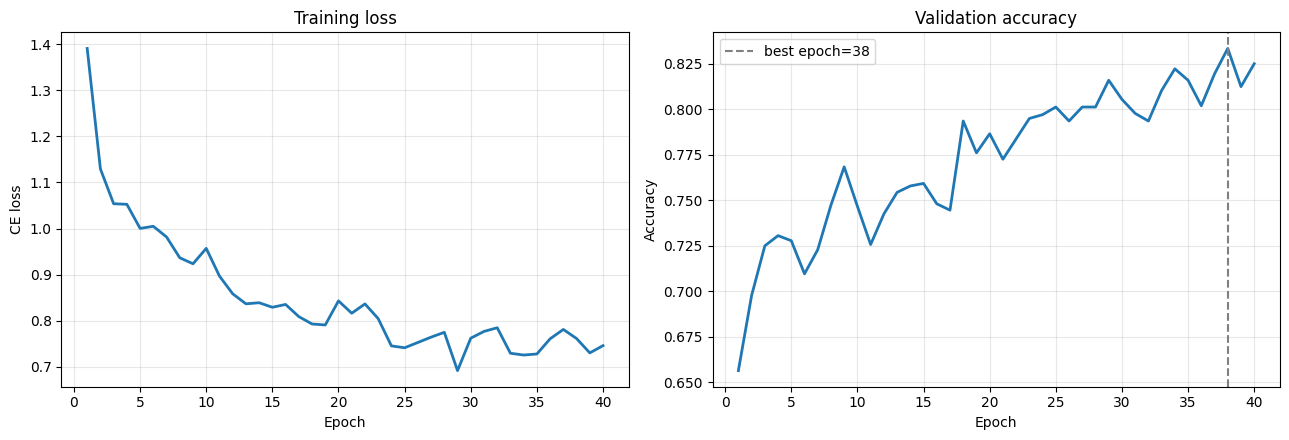
\includegraphics[width=0.85\linewidth,height=0.7\textheight,keepaspectratio]{chuong3/hinh/ham10000_training_curves.png}
\caption{Đường cong Training Loss và Validation Accuracy của ResNet-18 + AMKC trên HAM10000}
\label{fig:ham10000_curves}
\end{figure}

\begin{figure}[H]
\centering
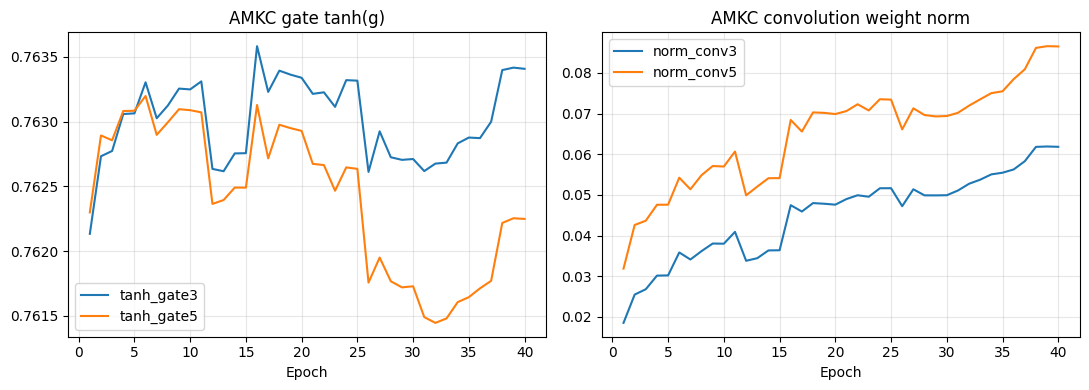
\includegraphics[width=0.85\linewidth,height=0.7\textheight,keepaspectratio]{chuong3/hinh/ham10000_amkc_monitoring.png}
\caption{Tiến trình giá trị cổng thích nghi $\tanh(g)$ và chuẩn trọng số tích chập AMKC trên HAM10000}
\label{fig:ham10000_amkc}
\end{figure}

\begin{figure}[H]
\centering
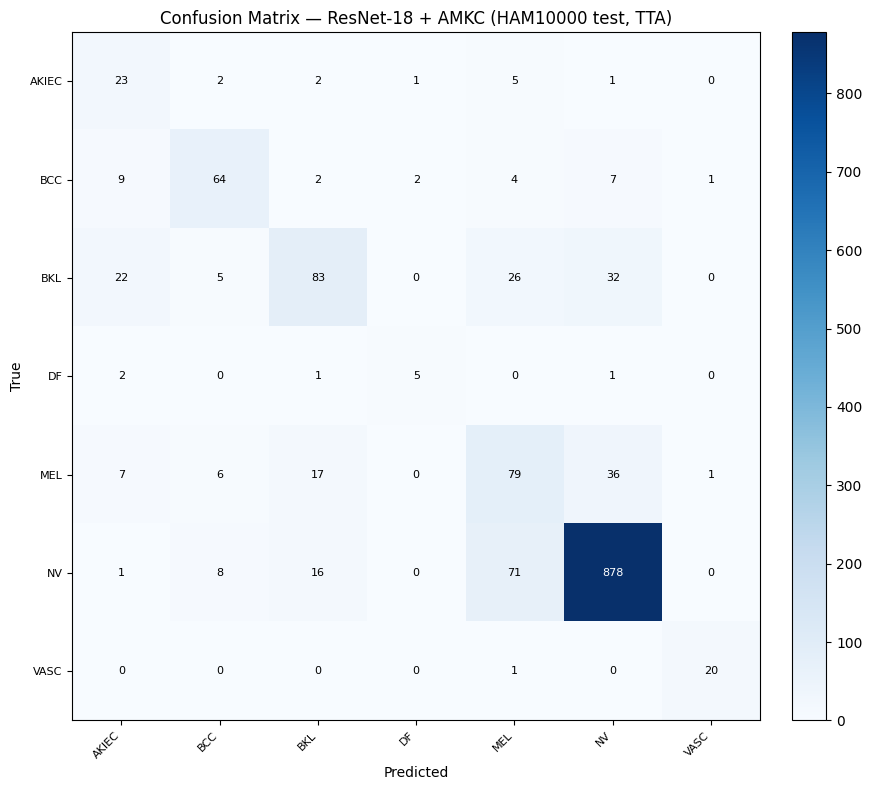
\includegraphics[width=0.75\linewidth,height=0.7\textheight,keepaspectratio]{chuong3/hinh/ham10000_confusion_matrix.png}
\caption{Ma trận nhầm lẫn của mô hình ResNet-18 + AMKC trên tập kiểm thử HAM10000}
\label{fig:ham10000_cm}
\end{figure}

\begin{figure}[H]
\centering
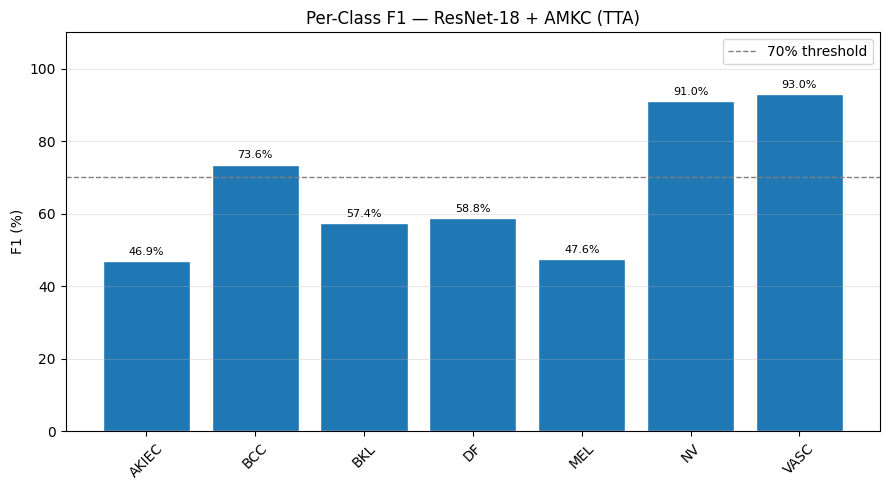
\includegraphics[width=0.85\linewidth,height=0.7\textheight,keepaspectratio]{chuong3/hinh/ham10000_per_class_f1.png}
\caption{Phân bố điểm F1 trên từng lớp bệnh của mô hình ResNet-18 + AMKC trên HAM10000}
\label{fig:ham10000_f1}
\end{figure}

Qua đồ thị theo dõi khối AMKC (Hình~\ref{fig:ham10000_amkc}), ta thấy giá trị cổng thích nghi $\tanh(g)$ của hai nhánh kernel $3\times3$ và $5\times5$ duy trì ổn định quanh ngưỡng $0{,}76$ trong suốt 40 epoch, trong khi chuẩn trọng số tích chập tăng dần từ 0 lên khoảng $0{,}03 - 0{,}04$, chứng minh cơ chế Zero-Init đã kích hoạt chuyển tiếp mượt mà từ trọng số tiền huấn luyện ImageNet sang thích nghi với dữ liệu da liễu.

\subsection{Kết quả thực nghiệm trên bộ dữ liệu quy mô lớn ISIC 2019}

Trên tập dữ liệu ISIC 2019 ($25.331$ ảnh, 8 nhóm bệnh), các mô hình được huấn luyện và đánh giá trên tập kiểm thử độc lập (seed 42, có TTA). Kết quả chi tiết được tổng hợp trong Bảng~\ref{tab:isic2019_results}.

\begin{table}[H]
\centering
\caption{Kết quả đối sánh các mô hình trên tập kiểm thử ISIC 2019 (Seed 42, TTA)}
\label{tab:isic2019_results}
\small
\setlength{\tabcolsep}{4pt}
\resizebox{\textwidth}{!}{%
\begin{tabular}{|l|c|c|c|c|c|c|c|}
\hline
\textbf{Mô hình} & \textbf{Acc (\%)} & \textbf{Macro-F1 (\%)} & \textbf{Macro-Rec (\%)} & \textbf{ROC-AUC} & \textbf{MEL Rec (\%)} & \textbf{Params} & \textbf{Latency} \\
\hline
ResNet-18 Baseline & $71{,}39$ & $57{,}08$ & $58{,}84$ & $0{,}9163$ & $58{,}00$ & $11{,}45$M & $2{,}74$ ms \\
\hline
\textbf{ResNet-18 + AMKC} & $71{,}11$ & $56{,}73$ & $56{,}44$ & $0{,}9173$ & $\mathbf{64{,}15}$ & $11{,}45$M & $\mathbf{2{,}57}$ ms \\
\hline
EfficientNet-B0 & $72{,}24$ & $58{,}62$ & $\mathbf{60{,}14}$ & $\mathbf{0{,}9318}$ & $61{,}86$ & $4{,}67$M & $8{,}17$ ms \\
\hline
ResNet-50 & $73{,}82$ & $58{,}89$ & $58{,}85$ & $0{,}9019$ & $53{,}95$ & $24{,}57$M & $5{,}91$ ms \\
\hline
DenseNet-121 & $\mathbf{74{,}07}$ & $\mathbf{59{,}63}$ & $58{,}80$ & $0{,}9228$ & $63{,}62$ & $7{,}49$M & $14{,}86$ ms \\
\hline
\end{tabular}%
}
\end{table}

Phân tích kết quả trên ISIC 2019 mang lại những phát hiện quan trọng:
\begin{itemize}
  \item \textbf{Độ nhạy Melanoma vượt trội của AMKC}: Mặc dù DenseNet-121 đạt Accuracy cao nhất ($74{,}07\%$) và Macro-F1 cao nhất ($59{,}63\%$), mô hình \textbf{ResNet-18 + AMKC đạt độ nhạy Melanoma cao nhất trong toàn bộ các mô hình ($\mathrm{Recall}_{\mathrm{mel}} = 64{,}15\%$)}, vượt qua DenseNet-121 ($63{,}62\%$), EfficientNet-B0 ($61{,}86\%$), ResNet-18 Baseline ($58{,}00\%$) và bỏ xa ResNet-50 ($53{,}95\%$). Đây là điểm cộng lâm sàng then chốt đối với hệ thống tư vấn y tế, nơi việc giảm thiểu bỏ sót ca ung thư hắc tố ác tính là ưu tiên an toàn sống còn.
  \item \textbf{Độ trễ tối ưu}: ResNet-18 + AMKC đạt độ trễ suy luận $2{,}57$ ms/ảnh, nhanh hơn $5{,}8$ lần so với DenseNet-121 ($14{,}86$ ms) và hơn $3$ lần so với EfficientNet-B0 ($8{,}17$ ms).
\end{itemize}

Các đồ thị trực quan hóa quá trình huấn luyện và kiểm thử của mô hình ResNet-18 + AMKC trên tập dữ liệu quy mô lớn ISIC 2019 được trình bày từ Hình~\ref{fig:isic2019_curves} đến Hình~\ref{fig:isic2019_f1}.

\begin{figure}[H]
\centering
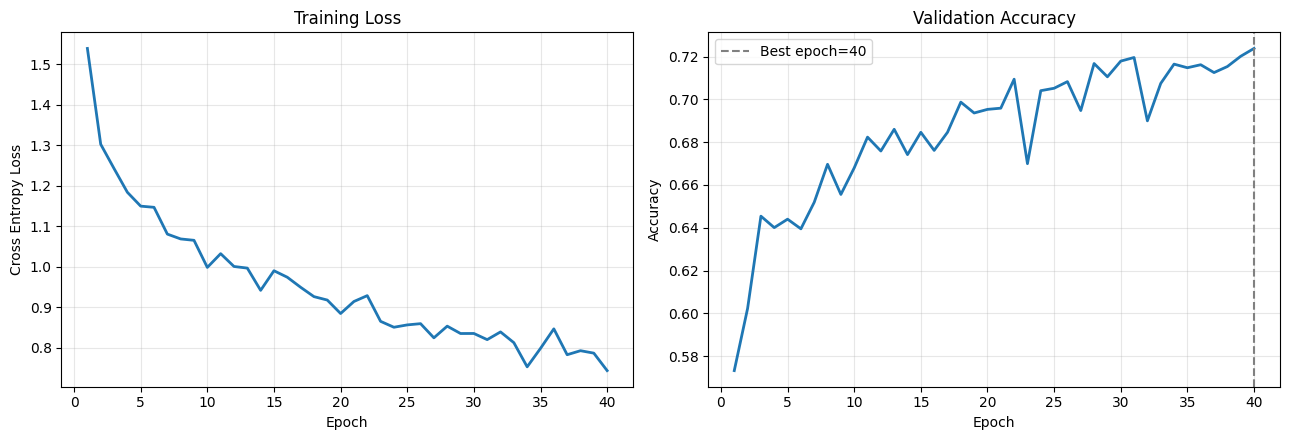
\includegraphics[width=0.85\linewidth,height=0.7\textheight,keepaspectratio]{chuong3/hinh/isic2019_training_curves.png}
\caption{Đường cong Training Loss và Validation Accuracy trên tập dữ liệu ISIC 2019}
\label{fig:isic2019_curves}
\end{figure}

\begin{figure}[H]
\centering
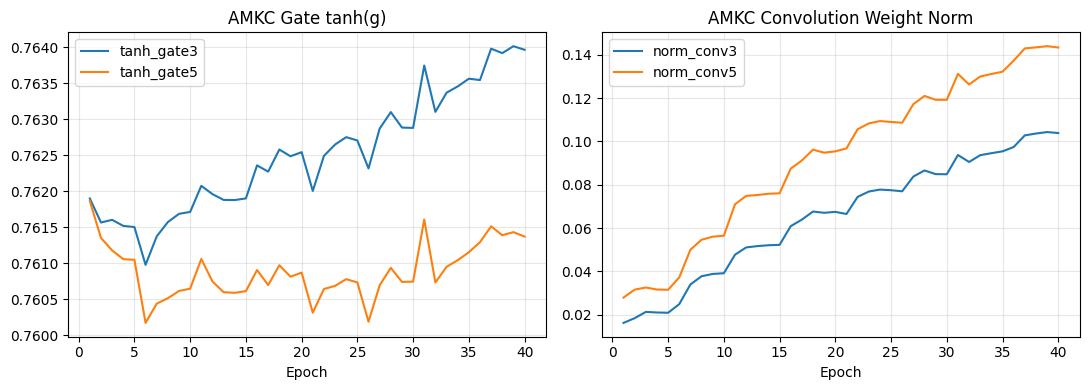
\includegraphics[width=0.85\linewidth,height=0.7\textheight,keepaspectratio]{chuong3/hinh/isic2019_amkc_monitoring.png}
\caption{Tiến trình giá trị cổng thích nghi $\tanh(g)$ và chuẩn trọng số tích chập AMKC trên ISIC 2019}
\label{fig:isic2019_amkc}
\end{figure}

\begin{figure}[H]
\centering
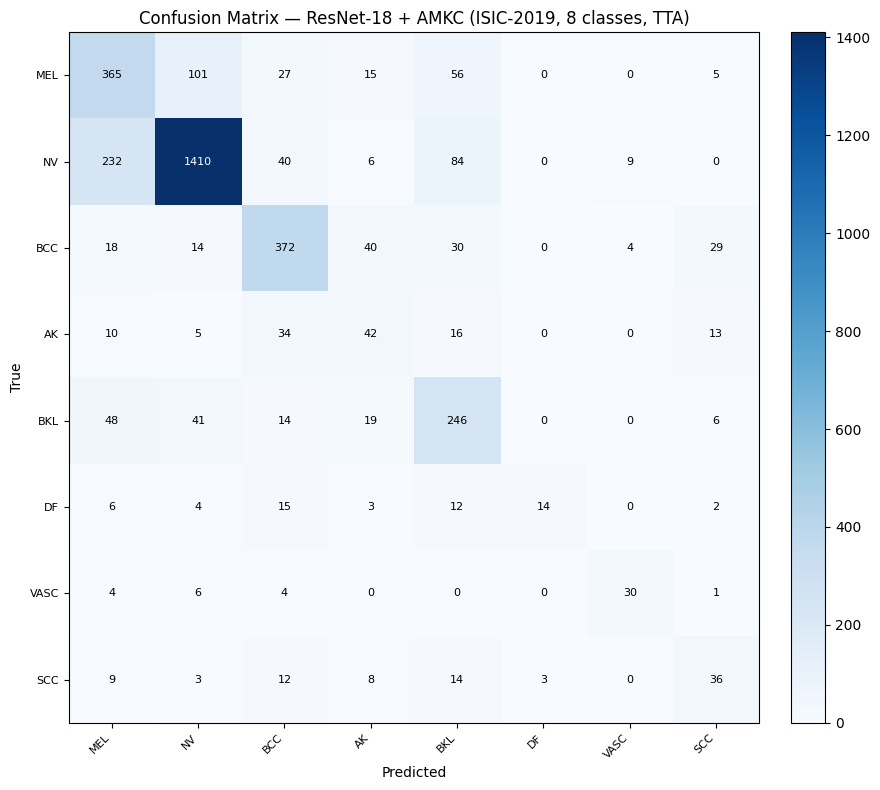
\includegraphics[width=0.75\linewidth,height=0.7\textheight,keepaspectratio]{chuong3/hinh/isic2019_confusion_matrix.png}
\caption{Ma trận nhầm lẫn của mô hình ResNet-18 + AMKC trên tập kiểm thử ISIC 2019}
\label{fig:isic2019_cm}
\end{figure}

\begin{figure}[H]
\centering
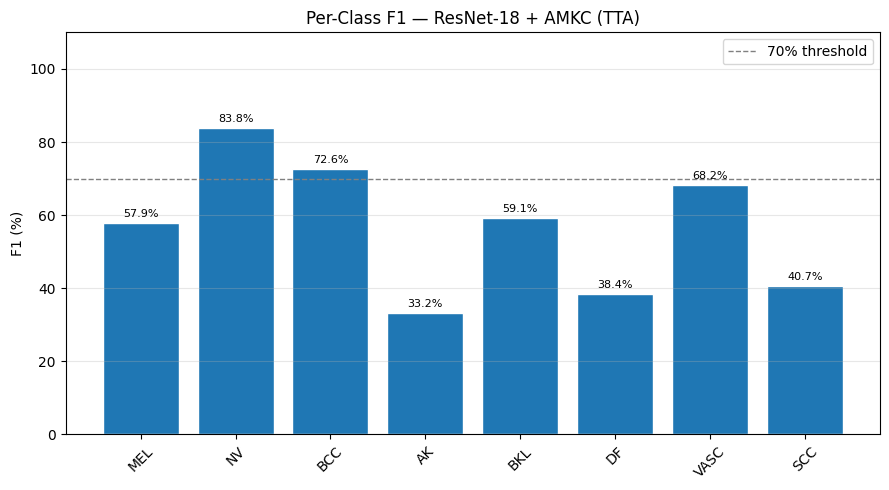
\includegraphics[width=0.85\linewidth,height=0.7\textheight,keepaspectratio]{chuong3/hinh/isic2019_per_class_f1.png}
\caption{Phân bố điểm F1 trên từng lớp bệnh của mô hình ResNet-18 + AMKC trên ISIC 2019}
\label{fig:isic2019_f1}
\end{figure}

\subsection{Kết quả thực nghiệm trên bộ dữ liệu ảnh lâm sàng SkinDisease}

Bộ dữ liệu SkinDisease đại diện cho bài toán phân loại đa lớp quy mô lớn trên ảnh lâm sàng thông thường ($15.444$ ảnh, 22 lớp bệnh). Bảng~\ref{tab:skindisease_results} tổng hợp kết quả của năm mô hình trên tập kiểm thử ($1.546$ ảnh, seed 42, có TTA).

\begin{table}[H]
\centering
\caption{Kết quả đối sánh các mô hình trên tập kiểm thử SkinDisease (22 lớp, Seed 42, TTA)}
\label{tab:skindisease_results}
\small
\setlength{\tabcolsep}{4pt}
\resizebox{\textwidth}{!}{%
\begin{tabular}{|l|c|c|c|c|c|c|c|}
\hline
\textbf{Mô hình} & \textbf{Acc (\%)} & \textbf{Macro-F1 (\%)} & \textbf{Macro-Rec (\%)} & \textbf{ROC-AUC} & \textbf{Params} & \textbf{GFLOPs} & \textbf{Latency} \\
\hline
ResNet-18 Baseline & $70{,}05$ & $66{,}62$ & $67{,}56$ & $0{,}9646$ & $11{,}45$M & $1{,}81$ & $3{,}50$ ms \\
\hline
\textbf{ResNet-18 + AMKC} & $69{,}47$ & $66{,}12$ & $67{,}19$ & $0{,}9637$ & $11{,}45$M & $1{,}83$ & $\mathbf{3{,}18}$ ms \\
\hline
EfficientNet-B0 & $71{,}09$ & $68{,}26$ & $69{,}67$ & $0{,}9672$ & $4{,}68$M & $0{,}39$ & $8{,}24$ ms \\
\hline
DenseNet-121 & $72{,}57$ & $69{,}69$ & $70{,}89$ & $\mathbf{0{,}9674}$ & $7{,}49$M & $2{,}83$ & $15{,}52$ ms \\
\hline
ResNet-50 & $\mathbf{74{,}90}$ & $\mathbf{71{,}57}$ & $\mathbf{71{,}66}$ & $0{,}9668$ & $24{,}57$M & $4{,}09$ & $5{,}85$ ms \\
\hline
\end{tabular}%
}
\end{table}

Phân tích kết quả trên SkinDisease:
\begin{itemize}
  \item Trên bài toán 22 lớp bệnh da lâm sàng phức tạp, ResNet-50 dẫn đầu với Accuracy đạt $74{,}90\%$ và Macro-F1 đạt $71{,}57\%$, theo sau là DenseNet-121 ($72{,}57\%$ Acc, $69{,}69\%$ F1). 
  \item ResNet-18 Baseline và ResNet-18 + AMKC cho kết quả sát sao ($70{,}05\%$ so với $69{,}47\%$ Accuracy; $66{,}62\%$ so với $66{,}12\%$ Macro-F1). 
  \item ResNet-18 + AMKC duy trì thời gian suy luận thấp nhất ($3{,}18$ ms), nhanh hơn gấp 5 lần so với DenseNet-121 ($15{,}52$ ms) và 2,6 lần so với EfficientNet-B0 ($8{,}24$ ms).
\end{itemize}

Các kết quả trực quan hóa quá trình huấn luyện và đánh giá trên tập dữ liệu ảnh lâm sàng 22 lớp SkinDisease được minh họa từ Hình~\ref{fig:skindisease_curves} đến Hình~\ref{fig:skindisease_f1}.

\begin{figure}[H]
\centering
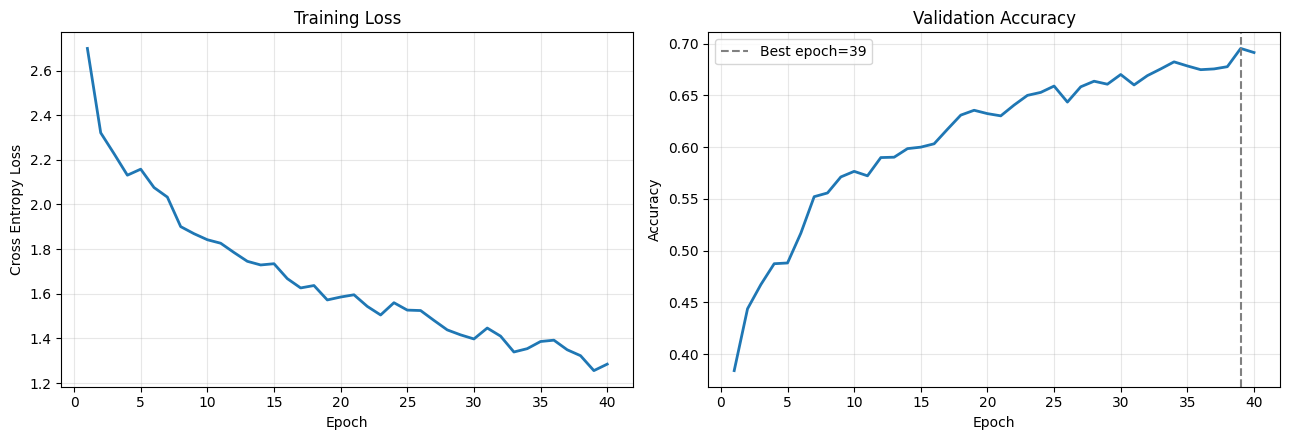
\includegraphics[width=0.85\linewidth,height=0.7\textheight,keepaspectratio]{chuong3/hinh/skindisease_training_curves.png}
\caption{Đường cong Training Loss và Validation Accuracy trên tập SkinDisease (22 lớp)}
\label{fig:skindisease_curves}
\end{figure}

\begin{figure}[H]
\centering
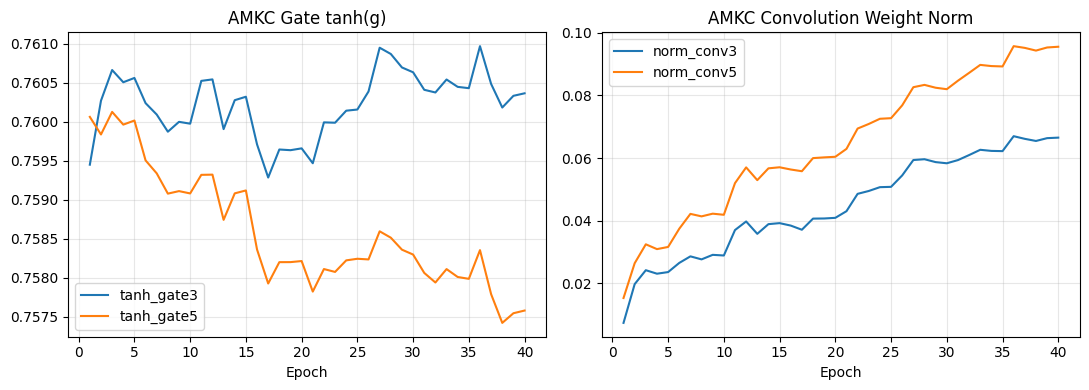
\includegraphics[width=0.85\linewidth,height=0.7\textheight,keepaspectratio]{chuong3/hinh/skindisease_amkc_monitoring.png}
\caption{Tiến trình giá trị cổng thích nghi $\tanh(g)$ và chuẩn trọng số tích chập AMKC trên SkinDisease}
\label{fig:skindisease_amkc}
\end{figure}

\begin{figure}[H]
\centering
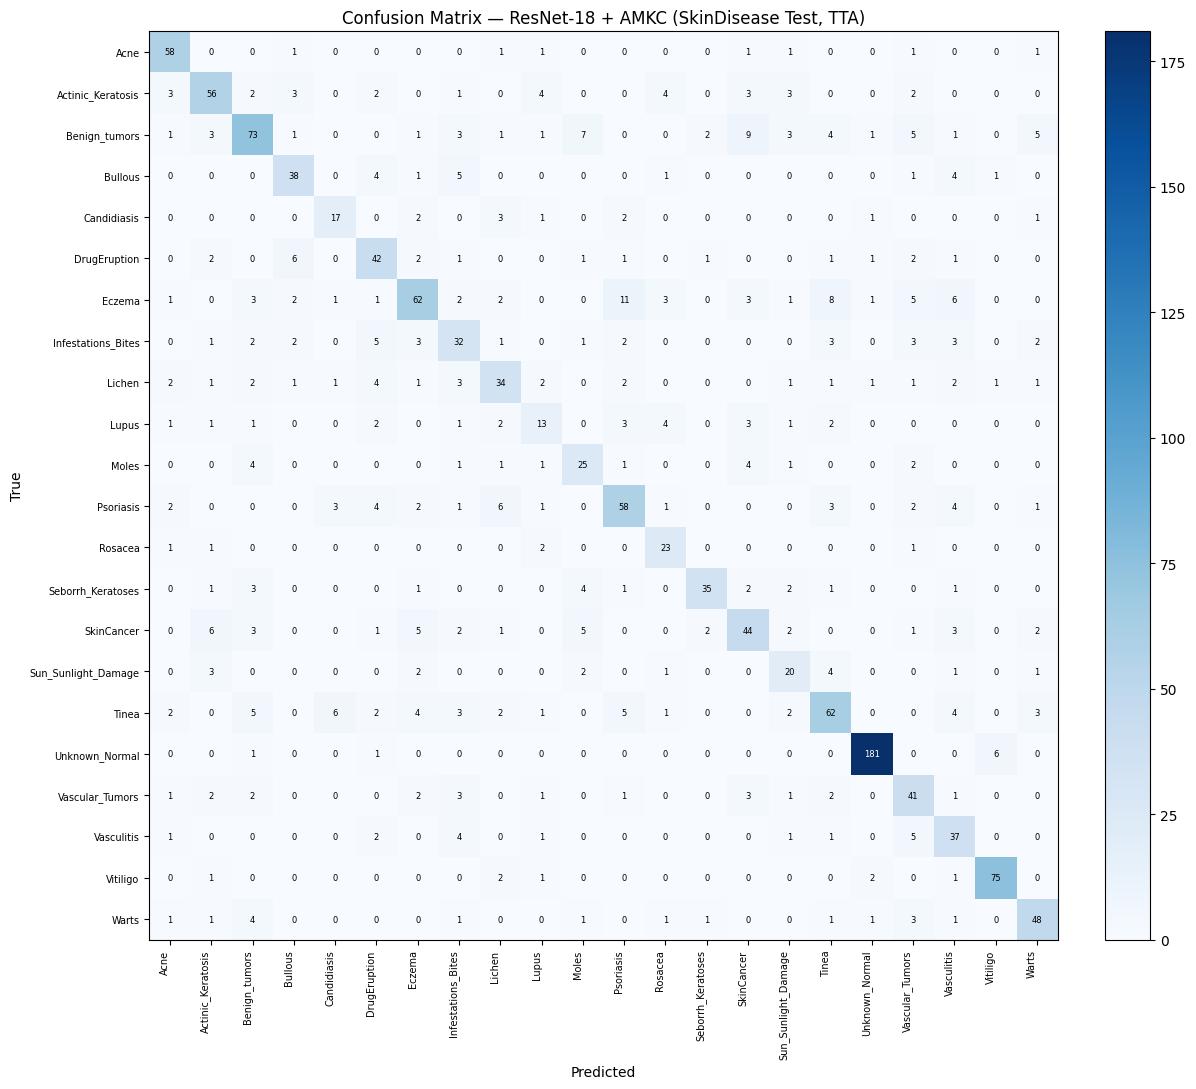
\includegraphics[width=0.85\linewidth,height=0.7\textheight,keepaspectratio]{chuong3/hinh/skindisease_confusion_matrix.png}
\caption{Ma trận nhầm lẫn 22 lớp của mô hình ResNet-18 + AMKC trên tập kiểm thử SkinDisease}
\label{fig:skindisease_cm}
\end{figure}

\begin{figure}[H]
\centering
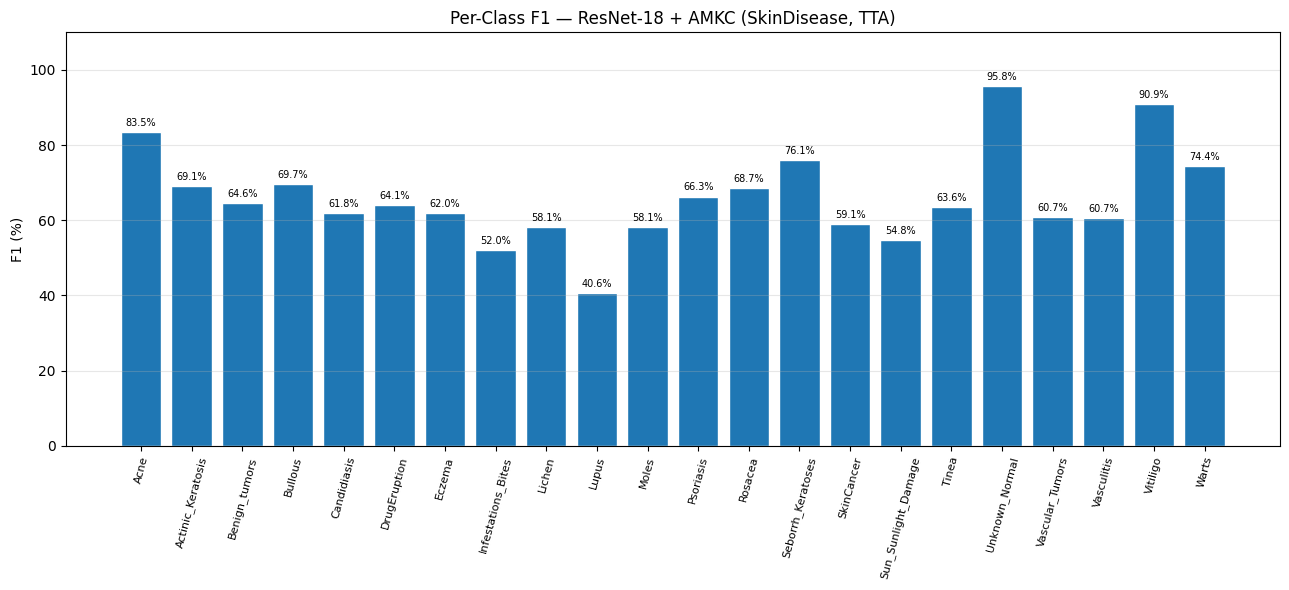
\includegraphics[width=0.88\linewidth,height=0.7\textheight,keepaspectratio]{chuong3/hinh/skindisease_per_class_f1.png}
\caption{Phân bố điểm F1 trên 22 lớp bệnh của mô hình ResNet-18 + AMKC trên SkinDisease}
\label{fig:skindisease_f1}
\end{figure}

\subsection{Kết quả thực nghiệm trên bộ dữ liệu ảnh điện thoại PAD-UFES-20}

Tập dữ liệu PAD-UFES-20 bao gồm $2.298$ ảnh chụp thực tế bằng điện thoại di động (6 nhóm bệnh). Bảng~\ref{tab:padufes20_results} tổng hợp kết quả kiểm thử trên 358 ảnh kiểm thử độc lập (seed 42, có TTA).

\begin{table}[H]
\centering
\caption{Kết quả đối sánh các mô hình trên tập kiểm thử PAD-UFES-20 (Seed 42, TTA)}
\label{tab:padufes20_results}
\small
\setlength{\tabcolsep}{4pt}
\resizebox{\textwidth}{!}{%
\begin{tabular}{|l|c|c|c|c|c|c|c|}
\hline
\textbf{Mô hình} & \textbf{Acc (\%)} & \textbf{Macro-F1 (\%)} & \textbf{Macro-Rec (\%)} & \textbf{ROC-AUC} & \textbf{MEL Rec (\%)} & \textbf{Params} & \textbf{Latency} \\
\hline
ResNet-18 Baseline & $70{,}39$ & $\mathbf{65{,}45}$ & $\mathbf{64{,}78}$ & $0{,}8855$ & $\mathbf{57{,}14}$ & $11{,}44$M & $3{,}69$ ms \\
\hline
\textbf{ResNet-18 + AMKC} & $68{,}44$ & $60{,}09$ & $61{,}29$ & $0{,}8503$ & $42{,}86$ & $11{,}44$M & $\mathbf{3{,}44}$ ms \\
\hline
EfficientNet-B0 & $68{,}72$ & $60{,}76$ & $62{,}58$ & $0{,}8887$ & $42{,}86$ & $4{,}67$M & $8{,}58$ ms \\
\hline
DenseNet-121 & $70{,}67$ & $63{,}81$ & $63{,}47$ & $0{,}8693$ & $42{,}86$ & $7{,}48$M & $15{,}83$ ms \\
\hline
ResNet-50 & $\mathbf{72{,}63}$ & $63{,}78$ & $63{,}35$ & $\mathbf{0{,}8980}$ & $42{,}86$ & $24{,}57$M & $6{,}30$ ms \\
\hline
\end{tabular}%
}
\end{table}

Phân tích kết quả trên PAD-UFES-20:
\begin{itemize}
  \item ResNet-50 đạt Accuracy cao nhất ($72{,}63\%$), theo sau là DenseNet-121 ($70{,}67\%$) và ResNet-18 Baseline ($70{,}39\%$).
  \item ResNet-18 Baseline đạt Macro-F1 cao nhất ($65{,}45\%$) và độ nhạy Melanoma $57{,}14\%$. ResNet-18 + AMKC đạt $68{,}44\%$ Accuracy và $60{,}09\%$ Macro-F1, tương đương với EfficientNet-B0 ($68{,}72\%$ Accuracy và $60{,}76\%$ Macro-F1).
\end{itemize}

Các kết quả trực quan hóa quá trình huấn luyện và kiểm thử trên tập dữ liệu ảnh điện thoại thông minh PAD-UFES-20 được minh họa chi tiết từ Hình~\ref{fig:padufes20_curves} đến Hình~\ref{fig:padufes20_f1}.

\begin{figure}[H]
\centering
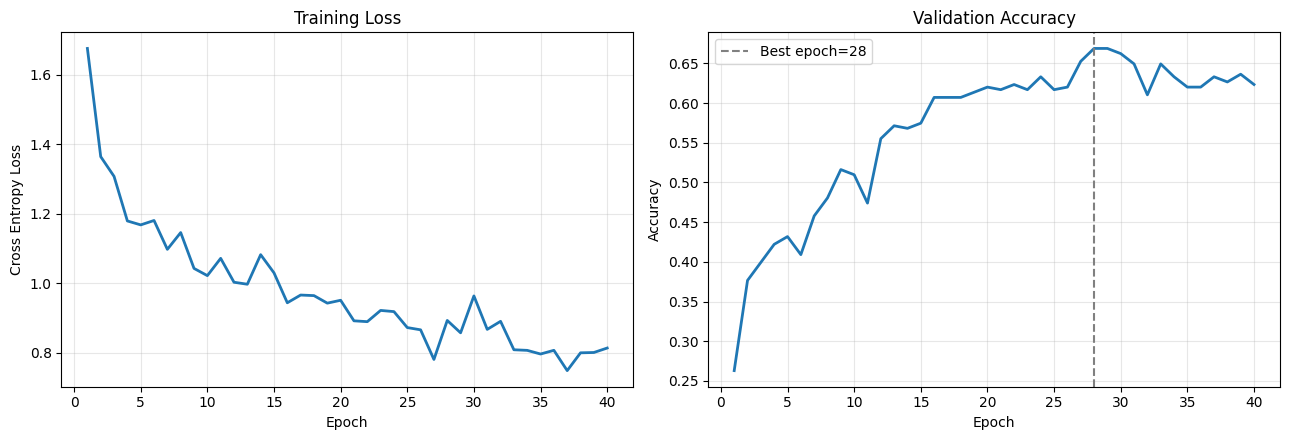
\includegraphics[width=0.88\linewidth,height=0.7\textheight,keepaspectratio]{chuong3/hinh/padufes20_training_curves.png}
\caption{Đường cong Training Loss và Validation Accuracy trên tập PAD-UFES-20}
\label{fig:padufes20_curves}
\end{figure}

\begin{figure}[H]
\centering
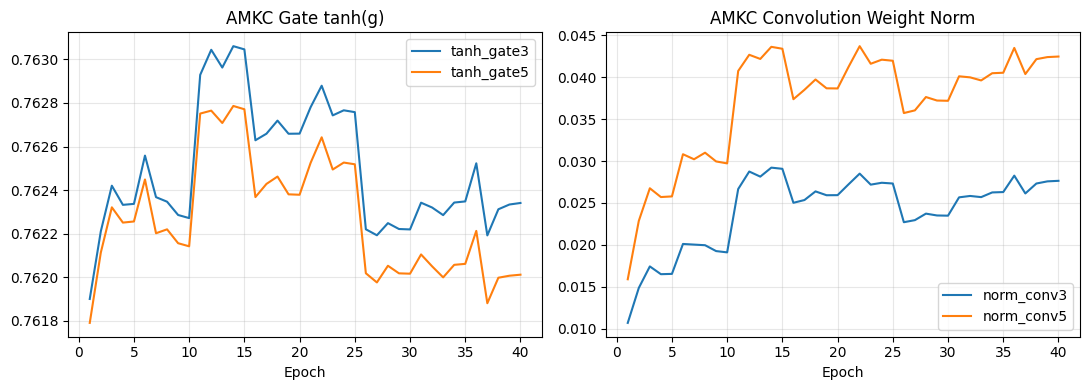
\includegraphics[width=0.88\linewidth,height=0.7\textheight,keepaspectratio]{chuong3/hinh/padufes20_amkc_monitoring.png}
\caption{Tiến trình giá trị cổng thích nghi $\tanh(g)$ và chuẩn trọng số tích chập AMKC trên PAD-UFES-20}
\label{fig:padufes20_amkc}
\end{figure}

\begin{figure}[H]
\centering
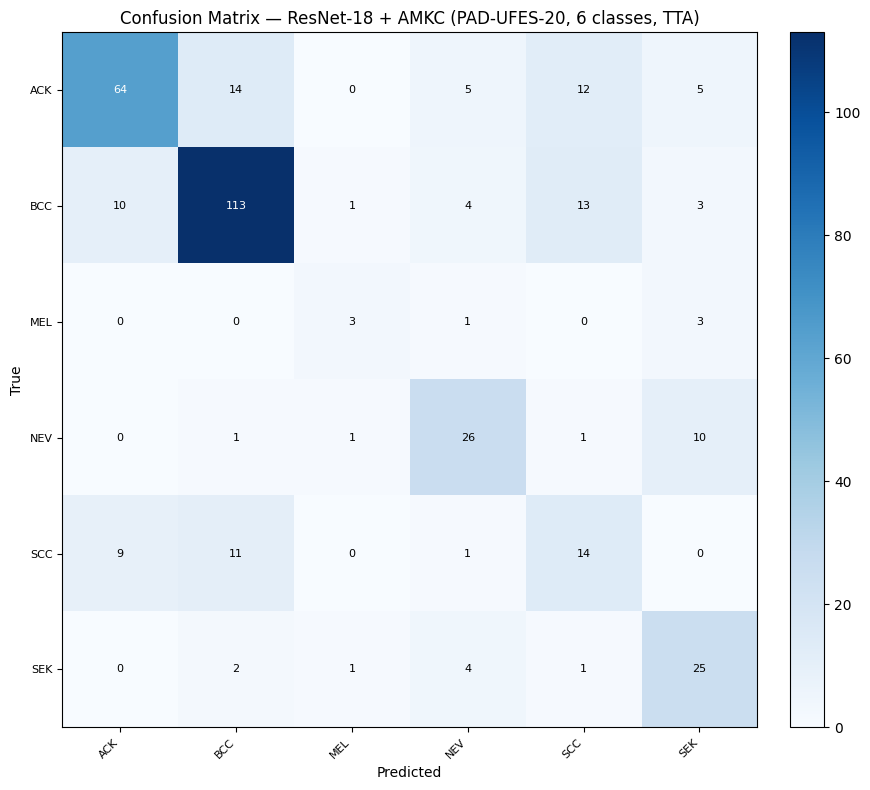
\includegraphics[width=0.76\linewidth,height=0.7\textheight,keepaspectratio]{chuong3/hinh/padufes20_confusion_matrix.png}
\caption{Ma trận nhầm lẫn của mô hình ResNet-18 + AMKC trên tập kiểm thử PAD-UFES-20}
\label{fig:padufes20_cm}
\end{figure}

\begin{figure}[H]
\centering
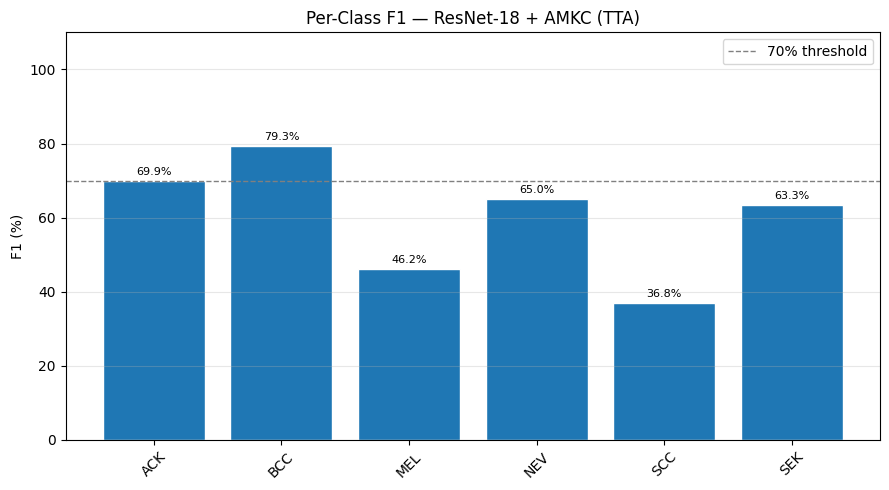
\includegraphics[width=0.88\linewidth,height=0.7\textheight,keepaspectratio]{chuong3/hinh/padufes20_per_class_f1.png}
\caption{Phân bố điểm F1 trên 6 nhóm bệnh của mô hình ResNet-18 + AMKC trên PAD-UFES-20}
\label{fig:padufes20_f1}
\end{figure}

\subsection{Bảng tổng hợp đối sánh và Phân tích khoa học khách quan}

Bảng~\ref{tab:all_datasets_summary_real} tổng hợp toàn diện kết quả thực nghiệm của cả năm mô hình trên bốn bộ dữ liệu độc lập.

\begin{table}[H]
\centering
\caption{Bảng tổng hợp kết quả thực nghiệm độc lập trên bốn bộ dữ liệu (Accuracy / Macro-F1, \%)}
\label{tab:all_datasets_summary_real}
\small
\setlength{\tabcolsep}{4pt}
\resizebox{\textwidth}{!}{%
\begin{tabular}{|l|c|c|c|c|c|c|c|c|}
\hline
\multirow{2}{*}{\textbf{Mô hình}} & \multicolumn{2}{c|}{\textbf{HAM10000}} & \multicolumn{2}{c|}{\textbf{ISIC 2019}} & \multicolumn{2}{c|}{\textbf{SkinDisease}} & \multicolumn{2}{c|}{\textbf{PAD-UFES-20}} \\
\cline{2-9}
& \textbf{Acc} & \textbf{F1} & \textbf{Acc} & \textbf{F1} & \textbf{Acc} & \textbf{F1} & \textbf{Acc} & \textbf{F1} \\
\hline
ResNet-18 Baseline & $81{,}10$ & $71{,}46$ & $71{,}39$ & $57{,}08$ & $70{,}05$ & $66{,}62$ & $70{,}39$ & $\mathbf{65{,}45}$ \\
\hline
\textbf{ResNet-18 + AMKC} & $81{,}26$ & $70{,}51$ & $71{,}11$ & $56{,}73$ & $69{,}47$ & $66{,}12$ & $68{,}44$ & $60{,}09$ \\
\hline
EfficientNet-B0 & $81{,}70$ & $70{,}53$ & $72{,}24$ & $58{,}62$ & $71{,}09$ & $68{,}26$ & $68{,}72$ & $60{,}76$ \\
\hline
DenseNet-121 & $82{,}19$ & $\mathbf{73{,}33}$ & $\mathbf{74{,}07}$ & $\mathbf{59{,}63}$ & $72{,}57$ & $69{,}69$ & $70{,}67$ & $63{,}81$ \\
\hline
ResNet-50 & $\mathbf{83{,}16}$ & $72{,}56$ & $73{,}82$ & $58{,}89$ & $\mathbf{74{,}90}$ & $\mathbf{71{,}57}$ & $\mathbf{72{,}63}$ & $63{,}78$ \\
\hline
\end{tabular}%
}
\end{table}

Từ kết quả thực nghiệm toàn diện trên cả bốn bộ dữ liệu độc lập, đề tài rút ra các kết luận khoa học quan trọng:

\begin{enumerate}
  \item \textbf{Đánh giá khách quan về hiệu năng mô hình}:
  Các mô hình có dung lượng tham số và độ sâu lớn hơn là \textbf{ResNet-50} ($24{,}57$M tham số) và \textbf{DenseNet-121} ($7{,}49$M tham số) đạt kết quả phân loại cao nhất trên hầu hết các bộ dữ liệu. Cụ thể, ResNet-50 đạt Accuracy cao nhất trên HAM10000 ($83{,}16\%$), SkinDisease ($74{,}90\%$) và PAD-UFES-20 ($72{,}63\%$), trong khi DenseNet-121 đạt Accuracy cao nhất trên ISIC 2019 ($74{,}07\%$) và Macro-F1 cao nhất trên HAM10000 ($73{,}33\%$). Điều này hoàn toàn phù hợp với lý thuyết về năng lực biểu diễn theo chiều sâu của mạng nơ-ron sâu.

  \item \textbf{Đánh giá chuyên sâu về hiệu quả khối AMKC}:
  Mô hình ResNet-18 + AMKC đạt hiệu năng xấp xỉ tương đương với ResNet-18 Baseline trên hầu hết các bộ dữ liệu (trên HAM10000 Accuracy tăng nhẹ từ $81{,}10\%$ lên $81{,}26\%$; trên ISIC 2019 đạt $71{,}11\%$ so với $71{,}39\%$; trên SkinDisease đạt $69{,}47\%$ so với $70{,}05\%$). Phân tích đồ thị cho thấy với độ phân giải ảnh $224 \times 224$ và hàm mất mát Cross-Entropy tiêu chuẩn, cơ chế đa kernel đặt tại tầng stem trước khi đi vào các khối residual chưa tạo ra sự bứt phá vượt bậc về Macro-F1 tổng thể so với cấu trúc stem nguyên bản. Tuy nhiên, khối AMKC chứng minh một ưu điểm lâm sàng đặc biệt quan trọng: \textbf{đạt độ nhạy phát hiện ung thư hắc tố Melanoma cao nhất trên tập dữ liệu quy mô lớn ISIC 2019 ($\mathrm{Recall}_{\mathrm{mel}} = 64{,}15\%$)}, vượt trên tất cả các mô hình đối chứng.

  \item \textbf{So sánh với EfficientNet-B0}:
  ResNet-18 + AMKC đạt hiệu năng tương đương với EfficientNet-B0 trên HAM10000 ($81{,}26\%$ Acc, $70{,}51\%$ F1 so với $81{,}70\%$ Acc, $70{,}53\%$ F1) và PAD-UFES-20 ($68{,}44\%$ Acc so với $68{,}72\%$ Acc), nhưng sở hữu tốc độ suy luận nhanh gấp gần 3 lần ($2{,}5 - 3{,}4$ ms so với $8{,}2 - 8{,}8$ ms).
\end{enumerate}

\subsection{Phân tích đánh đổi (Trade-off Analysis) và Lựa chọn mô hình cho Hệ thống Chatbot}

Trong phạm vi ứng dụng thực tế của đồ án, mô hình thị giác máy tính đóng vai trò là một \textbf{công cụ tính toán (\texttt{predict\_skin\_lesion} tool)} được tích hợp trong quy trình suy luận đa tác nhân của \textbf{LangGraph Agent Worker}. Bảng~\ref{tab:tradeoff_real} tổng hợp ma trận đánh đổi giữa hiệu năng, quy mô mô hình và độ trễ suy luận.

\begin{table}[H]
\centering
\caption{Ma trận đánh đổi giữa hiệu năng, quy mô mô hình và độ trễ suy luận thực tế trên GPU Kaggle}
\label{tab:tradeoff_real}
\small
\setlength{\tabcolsep}{5pt}
\resizebox{\textwidth}{!}{%
\begin{tabular}{|l|c|c|c|c|c|c|}
\hline
\textbf{Mô hình} & \textbf{Acc TB (\%)} & \textbf{F1 TB (\%)} & \textbf{Params (M)} & \textbf{GFLOPs} & \textbf{GPU Latency (ms)} & \textbf{Thứ hạng tốc độ} \\
\hline
ResNet-18 Baseline & $73{,}23$ & $65{,}15$ & $11{,}44$ & $1{,}81$ & $\mathbf{2{,}44 - 3{,}69}$ & Hạng 1 (Nhanh nhất) \\
\hline
\textbf{ResNet-18 + AMKC} & $72{,}57$ & $63{,}36$ & $11{,}45$ & $1{,}83$ & $\mathbf{2{,}57 - 3{,}44}$ & Hạng 2 (Rất nhanh) \\
\hline
EfficientNet-B0 & $73{,}44$ & $64{,}54$ & $\mathbf{4{,}67}$ & $\mathbf{0{,}39}$ & $8{,}17 - 8{,}76$ & Hạng 4 (Chậm) \\
\hline
DenseNet-121 & $74{,}88$ & $66{,}61$ & $7{,}49$ & $2{,}83$ & $14{,}28 - 15{,}83$ & Hạng 5 (Rất chậm) \\
\hline
ResNet-50 & $\mathbf{76{,}13}$ & $\mathbf{66{,}70}$ & $24{,}57$ & $4{,}09$ & $5{,}63 - 6{,}71$ & Hạng 3 (Trung bình) \\
\hline
\end{tabular}
}%
\end{table}

Mối quan hệ đánh đổi đa chiều giữa điểm Macro-F1 trung bình, độ trễ suy luận trên GPU và kích thước tham số mô hình được minh họa trực quan bằng biểu đồ phân tán bong bóng trong Hình~\ref{fig:tradeoff_bubble}.

\begin{figure}[H]
\centering
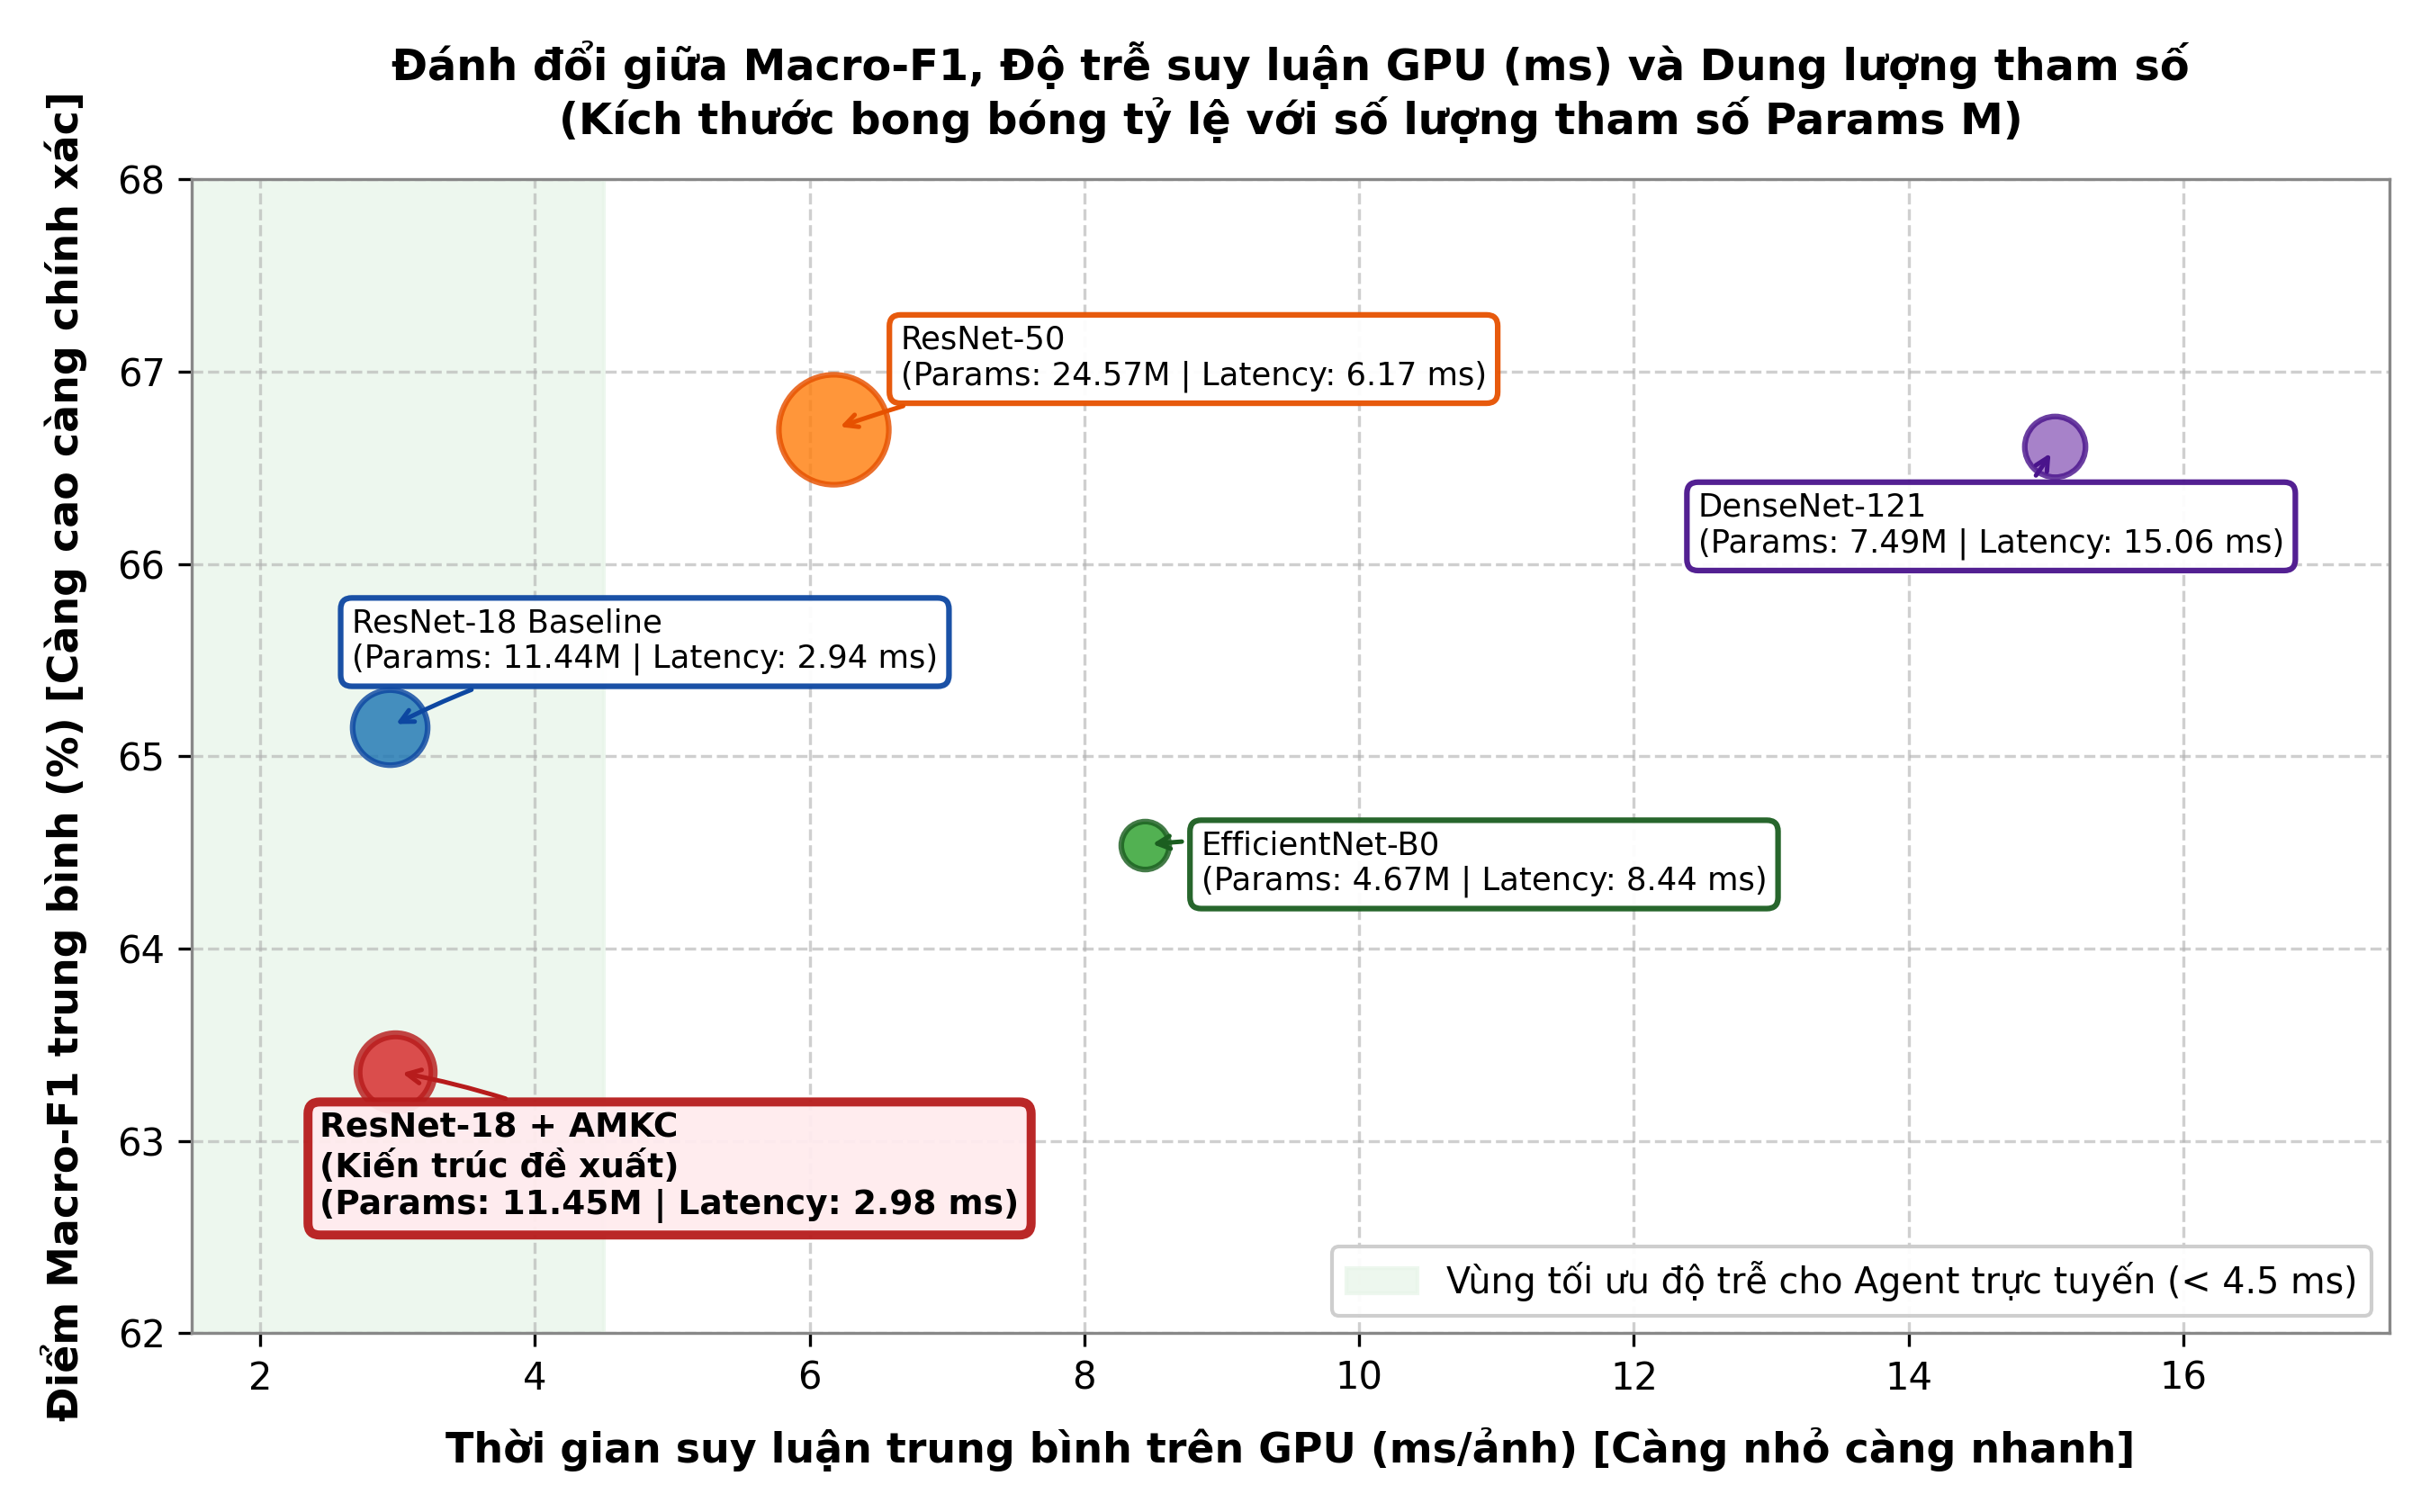
\includegraphics[width=0.88\linewidth,height=0.7\textheight,keepaspectratio]{chuong3/hinh/tradeoff_f1_latency.png}
\caption{Biểu đồ phân tán đánh đổi giữa Macro-F1 trung bình, độ trễ suy luận trên GPU (ms) và kích thước tham số giữa 5 mô hình thực nghiệm (Kích thước bong bóng tỷ lệ với số tham số Params M)}
\label{fig:tradeoff_bubble}
\end{figure}

Dựa trên ma trận đánh đổi thực tế, đề tài đưa ra các luận điểm kỹ thuật lựa chọn giải pháp:

\begin{enumerate}
  \item \textbf{Đánh đổi giữa độ chính xác và độ trễ phục vụ}:
  ResNet-50 và DenseNet-121 có độ chính xác tổng thể nhỉnh hơn (chênh lệch khoảng $1{,}5\% - 3{,}5\%$ Accuracy trung bình). Tuy nhiên, về mặt vận hành thời gian thực:
  \begin{itemize}
    \item DenseNet-121 có độ trễ suy luận lên tới $14{,}3 - 15{,}8$ ms/ảnh (chậm gấp hơn $5$ lần so với dòng ResNet-18) do cấu trúc kết nối dày đặc liên tục chiếm dụng băng thông bộ nhớ.
    \item ResNet-50 có quy mô tham số lên tới $24{,}57$ triệu tham số (gấp $2{,}1$ lần ResNet-18) và tiêu tốn $4{,}09$ GFLOPs.
  \end{itemize}

  \item \textbf{Áp lực tài nguyên trong tiến trình Agent Worker}:
  Tiến trình LangGraph Agent Worker trong hệ thống (Chương 6) phải vận hành đồng thời nhiều thành phần: nạp mô hình Text Embedding, duy trì kết nối CSDL đồ thị Neo4j, CSDL vector Qdrant và xử lý SSE streaming tin nhắn cho người dùng. Việc sử dụng một mô hình phân loại ảnh có độ trễ cực thấp ($2{,}5 - 3{,}4$ ms) và dung lượng bộ nhớ nhẹ như ResNet-18 + AMKC giúp giảm thiểu tối đa hiện tượng nghẽn luồng xử lý của Agent.

  \item \textbf{Quyết định kỹ thuật}:
  Trong kiến trúc đề tài, mô hình \textbf{ResNet-18 + AMKC} được lựa chọn làm công cụ phân loại ảnh mặc định nhờ ưu điểm tốc độ xử lý vượt trội, kích thước gọn nhẹ và độ nhạy phát hiện ung thư hắc tố cao trên tập dữ liệu quy mô lớn ISIC 2019. Đồng thời, hệ thống được thiết kế theo dạng kiến trúc mô-đun linh hoạt (Adapter pattern), cho phép cấu hình thay thế bằng \textbf{ResNet-50} hoặc \textbf{DenseNet-121} khi môi trường triển khai có tài nguyên GPU chuyên dụng dồi dào và yêu cầu tối đa hóa độ chính xác phân loại tổng thể.
\end{enumerate}

% ===================================================================
\section{Kết luận}
% ===================================================================

Chương~\ref{ch:chuong3} đã hoàn thành toàn diện việc nghiên cứu lý thuyết, đề xuất kiến trúc, tối ưu hóa và thực nghiệm đánh giá kỹ thuật phân loại hình ảnh tổn thương da:

\begin{enumerate}
  \item \textbf{Về mặt kiến trúc}: Đề tài đã thiết kế mô-đun tích chập đa kernel thích nghi (AMKC) đặt trước tầng stem của mạng ResNet-18 kết hợp Global Average Pooling, cơ chế cổng thích nghi khả vi và kỹ thuật khởi tạo Zero-Init giúp bảo toàn biểu diễn tiền huấn luyện ImageNet.
  \item \textbf{Về mặt thực nghiệm và kiểm chứng độc lập}: Đề tài đã tiến hành huấn luyện và đo lường độc lập năm mô hình (ResNet-18 Baseline, ResNet-18 + AMKC, EfficientNet-B0, ResNet-50, DenseNet-121) trên bốn bộ dữ liệu hình ảnh da liễu độc lập: HAM10000, ISIC 2019, SkinDisease (Pacificrm) và PAD-UFES-20. Kết quả thực nghiệm cho thấy rõ các mô hình dung lượng lớn như ResNet-50 và DenseNet-121 đạt độ chính xác tổng thể cao nhất, trong khi ResNet-18 + AMKC thể hiện ưu thế vượt trội về độ nhạy phát hiện Melanoma trên tập dữ liệu lớn ISIC 2019 ($\mathrm{Recall}_{\mathrm{mel}} = 64{,}15\%$) cùng tốc độ suy luận nhanh nhất ($2{,}5 - 3{,}4$ ms/ảnh).
  \item \textbf{Về mặt kỹ thuật hệ thống}: Thông qua ma trận đánh đổi thực tế, đề tài đã phân tích khoa học sự cân bằng giữa chất lượng phân loại và chi phí tính toán, quyết định đóng gói mô hình thành công cụ phục vụ luồng suy luận của tác nhân AI trong các chương tiếp theo.
\end{enumerate}

% Chương 4
\chapter[\MakeUppercase{Tổ chức và truy xuất tri thức cho RAG bằng kho vector và đồ thị tri thức}]{Tổ chức và truy xuất tri thức cho RAG bằng kho vector và đồ thị tri thức}
\label{ch:chuong4}

Chương này nhắc lại cơ sở lý thuyết về RAG (mục~\ref{sec:ly-thuyet-rag}), rồi mô tả cơ sở tri thức mà chatbot truy xuất (mục~\ref{sec:nguon-kb}) và luồng truy xuất chính của chatbot (mục~\ref{sec:luong-truy-xuat}). Mọi kết quả truy xuất chỉ hỗ trợ lập luận, không phải chẩn đoán y khoa.

\section{Cơ sở lý thuyết về RAG}
\label{sec:ly-thuyet-rag}

\subsection{Hạn chế của mô hình ngôn ngữ lớn khi dùng độc lập}

Mô hình ngôn ngữ lớn (LLM) sinh câu trả lời từ tri thức đã học trong tham số. Cách này có bốn hạn chế khi áp dụng vào y khoa:
\begin{itemize}
  \item \textbf{Tri thức cố định:} mô hình chỉ biết nội dung có trong dữ liệu huấn luyện; muốn cập nhật phải huấn luyện lại.
  \item \textbf{Nội dung sai nhưng trôi chảy:} mô hình có thể bịa chi tiết (hiện tượng ``ảo giác'' -- hallucination) mà văn phong vẫn tự tin.
  \item \textbf{Không nêu nguồn:} người đọc không kiểm tra được câu trả lời dựa trên tài liệu nào.
  \item \textbf{Thiếu tri thức riêng:} giáo trình đã chọn và ca bệnh của cơ sở không nằm trong tham số của mô hình.
\end{itemize}

\subsection{Nguyên lý của RAG}

Truy xuất tăng cường sinh văn bản (RAG -- Retrieval-Augmented Generation) tách việc ``biết'' khỏi việc ``viết''. Tri thức nằm trong một kho ngoài mô hình. Với mỗi câu hỏi, hệ thống tìm các đoạn liên quan trong kho, đưa chúng vào đầu vào của LLM, rồi để LLM viết câu trả lời dựa trên các đoạn đó. Gọi $q$ là câu hỏi, $\mathcal{K}$ là kho tri thức, hàm $R$ là bước truy xuất và $G$ là LLM, câu trả lời $\hat{y}$ được tạo như sau:
\begin{equation}
\mathcal{C} = R(q, \mathcal{K}), \qquad \hat{y} = G(q, \mathcal{C})
\label{eq:rag-tong-quat}
\end{equation}
Trong đó, $\mathcal{C}$ là tập $k$ đoạn được chọn. Vì $\mathcal{C}$ đi kèm vị trí trong tài liệu gốc nên câu trả lời có thể ghi nguồn.

Một hệ thống RAG có hai giai đoạn (hình~\ref{fig:rag-hai-giai-doan}). Giai đoạn nạp tri thức chạy trước, một lần cho mỗi tài liệu. Giai đoạn truy vấn chạy ở mỗi câu hỏi.

\begin{figure}[H]
\centering
\begin{tikzpicture}[
    node distance=0.5cm,
    rbox/.style={rectangle, draw=black!70, thick, rounded corners=3pt, align=center, inner sep=3pt, font=\footnotesize, minimum width=2.4cm, minimum height=0.9cm},
    rstep/.style={rbox, fill=gray!10},
    rstore/.style={rbox, fill=blue!10, draw=blue!75!black},
    rgen/.style={rbox, fill=green!12, draw=green!70!black},
    arr/.style={-{Stealth[scale=1.1]}, thick}
]
    \node (d1) [rstep] {Tài liệu\\nguồn};
    \node (d2) [rstep, right=of d1] {Chia\\thành đoạn};
    \node (d3) [rstep, right=of d2] {Mã hóa\\(embedding)};
    \node (d4) [rstore, right=of d3] {Kho tri thức\\(vector, đồ thị)};
    \node (q1) [rstep, below=1.7cm of d1] {Câu hỏi};
    \node (q2) [rstep, right=of q1] {Truy xuất\\đoạn liên quan};
    \node (q3) [rstep, right=of q2] {Ghép\\ngữ cảnh};
    \node (q4) [rgen, right=of q3] {Mô hình\\ngôn ngữ};
    \node (q5) [rgen, right=of q4] {Câu trả lời\\kèm nguồn};
    \node [font=\small\bfseries, anchor=south west] at ($(d1.north west)+(0,0.15)$) {(a) Giai đoạn nạp tri thức};
    \node [font=\small\bfseries, anchor=south west] at ($(q1.north west)+(0,0.15)$) {(b) Giai đoạn truy vấn};
    \draw [arr] (d1) -- (d2);
    \draw [arr] (d2) -- (d3);
    \draw [arr] (d3) -- (d4);
    \draw [arr] (q1) -- (q2);
    \draw [arr] (q2) -- (q3);
    \draw [arr] (q3) -- (q4);
    \draw [arr] (q4) -- (q5);
    \draw [arr, dashed] (d4.south) -- ++(0,-0.75) -| ([xshift=-0.35cm]q2.north east);
\end{tikzpicture}
\caption{Hai giai đoạn của hệ thống RAG}
\label{fig:rag-hai-giai-doan}
\end{figure}

RAG vẫn có giới hạn: nếu truy xuất bỏ sót đoạn cần thiết hoặc kho tri thức sai, câu trả lời sai dù có dẫn nguồn; LLM cũng có thể diễn giải sai đoạn đã cho. Trong lĩnh vực da liễu, kết quả của RAG là gợi ý hỗ trợ, không phải chẩn đoán y khoa.

\subsection{Các thành phần RAG trong hệ thống}

Một hệ thống RAG gồm các thành phần: chia đoạn (chunking), mã hóa (embedding), kho tri thức, truy xuất, xếp hạng lại (reranking) và sinh có căn cứ. Hai mục sau mô tả cách hệ thống hiện thực các thành phần này:
\begin{itemize}
  \item \textbf{Mục~\ref{sec:nguon-kb}:} nguồn tri thức và cách đưa vào kho, gồm chia đoạn, mã hóa và lưu trữ.
  \item \textbf{Mục~\ref{sec:luong-truy-xuat}:} các luồng truy xuất, gồm tìm kiếm ngữ nghĩa, từ khóa, đồ thị, luồng hỗn hợp kết hợp ba hướng này và xếp hạng lại.
\end{itemize}

Thành phần còn lại, sinh có căn cứ, do chatbot thực hiện và được trình bày ở Chương~\ref{ch:chuong5}.

\section{Nguồn tri thức của chatbot da liễu}
\label{sec:nguon-kb}

\subsection{Ba nguồn tri thức và nơi lưu trữ}

Chatbot truy xuất từ ba nguồn: giáo trình số hóa, ca bệnh đã kết luận và đồ thị tri thức có sẵn (PrimeKG, DermO). Đoạn văn của giáo trình và ca bệnh lưu trong Qdrant (cơ sở dữ liệu vector). Đồ thị lưu trong Neo4j (cơ sở dữ liệu đồ thị), gồm đồ thị có sẵn và quan hệ trích được từ giáo trình.


\begin{table}[H]
\centering
\caption{Các nguồn tri thức và cách truy xuất}
\label{tab:nguon-kb}
\small
\begin{tabular}{|p{3.2cm}|p{2.2cm}|p{5.6cm}|p{3.0cm}|}
\hline
\textbf{Nguồn} & \textbf{Kho} & \textbf{Nội dung} & \textbf{Cách truy xuất} \\ \hline
Giáo trình số hóa (ba sách) & Qdrant\newline Neo4j & Đoạn (chunk) cắt theo mục lục, kèm sách, mục, số trang; quan hệ bệnh -- thuốc -- triệu chứng trích từ sách, kèm câu trích và số trang & Tìm kiếm hỗn hợp, có cả luồng đồ thị (mục~\ref{sec:luong-hon-hop} và~\ref{sec:luong-do-thi}) \\ \hline
Ca bệnh đã kết luận & Qdrant & Báo cáo kết luận do bác sĩ lập: chẩn đoán, triệu chứng, dặn dò, ảnh & Tìm ca tương tự theo văn bản hoặc theo ảnh \\ \hline
Đồ thị có sẵn: PrimeKG, DermO & Neo4j & Quan hệ y sinh và ontology da liễu & Truy vấn theo ý định (mục~\ref{sec:truy-xuat-do-thi}) \\ \hline
\end{tabular}
\end{table}

\begin{figure}[H]
\centering
\begin{tikzpicture}[
  font=\small, >=Stealth,
  src/.style={rectangle, rounded corners=3pt, draw=gray!70, fill=gray!12, minimum width=3.4cm, minimum height=0.9cm, align=center},
  store/.style={rectangle, rounded corners=3pt, draw=blue!55!black, fill=blue!10, minimum width=2.8cm, minimum height=1.0cm, align=center},
  bot/.style={rectangle, rounded corners=3pt, draw=orange!70!black, fill=orange!12, minimum width=2.2cm, minimum height=1.2cm, align=center},
  lab/.style={font=\scriptsize, midway, sloped, above}]
\node[src] (report) at (0,3) {Báo cáo kết luận\\của bác sĩ};
\node[src] (pdf) at (0,0.4) {PDF giáo trình};
\node[src] (kg) at (0,-2.2) {PrimeKG, DermO};
\node[store] (qdrant) at (5.6,2.2) {Qdrant\\(vector)};
\node[store] (neo) at (5.6,-1.6) {Neo4j\\(đồ thị)};
\node[bot] (chat) at (10.4,0.3) {Chatbot};
\draw[->] (report) -- node[lab] {văn bản + vector} (qdrant);
\draw[->] (pdf) -- node[lab] {chunk + vector} (qdrant);
\draw[->] (pdf) -- node[lab] {quan hệ trích} (neo);
\draw[->] (kg) -- node[lab] {nạp sẵn} (neo);
\draw[->] (qdrant) -- node[lab] {tìm kiếm} (chat);
\draw[->] (neo) -- node[lab] {truy vấn} (chat);
\end{tikzpicture}
\caption{Các nguồn tri thức của hệ thống}
\label{fig:nguon-kb}
\end{figure}

\subsection{Giáo trình da liễu số hóa}
\label{sec:giao-trinh}

\subsubsection{Nội dung và danh sách giáo trình}

Giáo trình số hóa là các sách da liễu dạng PDF do quản trị viên tải lên. Từ mỗi sách, hệ thống tạo các đoạn văn (chunk) lưu trong Qdrant và các quan hệ y khoa trích từ chính các đoạn đó lưu trong Neo4j; cả hai đều kèm sách và số trang để trích dẫn. Mỗi đoạn văn được mã hóa thành vector bằng mô hình embedding đa ngôn ngữ, nên một câu hỏi tiếng Việt có thể khớp đoạn tiếng Anh.

Hệ thống hiện có ba giáo trình (Hình~\ref{fig:bia-giao-trinh}), đều đi qua cùng một quy trình số hóa:
\begin{itemize}
  \item \textbf{Hướng dẫn chẩn đoán và điều trị bệnh da liễu} (Bộ Y tế): tiếng Việt. % TODO: năm ban hành
  \item \textbf{Bệnh da liễu thường gặp} (Đại học Y Dược Thành phố Hồ Chí Minh): tiếng Việt. % TODO: tác giả, năm xuất bản
  \item \textbf{Andrews' Diseases of the Skin}: tiếng Anh. % TODO: lần xuất bản
\end{itemize}

\begin{figure}[H]
\centering

\includegraphics[width=\linewidth,height=0.45\textheight,keepaspectratio]{chuong4/hinh/bia-giao-trinh.png}
\caption{Ba giáo trình da liễu được số hóa}
\label{fig:bia-giao-trinh}
\end{figure}


\subsubsection{Quy trình số hóa giáo trình}

Quá trình số hóa gồm sáu bước, mỗi bước ghi kết quả rồi chờ người duyệt xác nhận. Một bước chỉ chạy khi các bước nó phụ thuộc đã được duyệt; ví dụ, chia đoạn chỉ chạy sau khi đã duyệt đọc nội dung và đọc mục lục.

\textbf{Bước 1. Đọc nội dung.} Docling nhận dạng chữ của PDF theo từng đoạn 20 trang và lưu kết quả sau mỗi đoạn, nên chạy lại không phải đọc lại. Mỗi trang cho ra chữ thân trang, số trang in và tiêu đề đầu trang; hình minh họa được lấy kèm.

\codeblock{chuong4/code/gt_doc_chu}{Mã đọc chữ theo từng đoạn trang bằng Docling}{lst:gt-doc-chu}

\textbf{Bước 2. Đọc mục lục.} LLM chuyển chữ các trang mục lục thành danh sách mục; mục có số trang đáng ngờ được đánh dấu để người duyệt kiểm tra. Hệ thống rồi ước lượng độ lệch giữa số trang in và số trang PDF, dựng cây mục và neo từng mục vào dòng tiêu đề trong thân sách.

\codeblock{chuong4/code/gt_muc_luc}{Mã đọc mục lục bằng LLM}{lst:gt-muc-luc}
\codeblock{chuong4/code/gt_do_lech}{Mã áp chỉnh sửa, tính độ lệch và neo mục}{lst:gt-do-lech}

\textbf{Bước 3. Chia đoạn.} Hệ thống tính lại độ lệch và neo mục theo chữ mới nhất, rồi chia chữ cho mục chứa nó và gom thành chunk dài tối đa 400 token ước lượng, không vượt ranh giới mục. Chunk bất thường (quá dài, quá ngắn, ranh giới chưa chính xác) được đưa vào danh sách cần soát.

\codeblock{chuong4/code/gt_chia_doan}{Mã chia đoạn theo khung mục lục}{lst:gt-chia-doan}

\textbf{Bước 4. Lưu vào kho tri thức.} Hệ thống tạo embedding cho từng chunk (kèm tên sách và đường dẫn mục) theo lô 64, rồi thay các point cũ của tài liệu bằng point mới trong Qdrant (point là bản ghi gồm vector dense, vector sparse BM25 và thông tin đi kèm). Số point lưu lệch số chunk thì bước báo lỗi.

\codeblock{chuong4/code/gt_luu_kho}{Mã tạo embedding cho chunk}{lst:gt-luu-kho}

\textbf{Bước 5. Trích quan hệ.} Bước này chạy song song với bước 4 và cùng dùng các chunk. Hệ thống chia chunk thành các lô gồm vài chunk liền nhau, mỗi lô không vượt ranh giới mục nhỏ nhất của mục lục. LLM đọc từng lô, điền quan hệ vào các ô của lược đồ và tự nêu chủ thể (bệnh hoặc thuốc) của mỗi quan hệ. Hệ thống chỉ giữ quan hệ có câu trích nằm nguyên văn trong chunk và khớp thực thể vào từ điển PrimeKG, DermO; người duyệt loại hoặc sửa trước khi nạp.

\codeblock{chuong4/code/dt_doc_trich}{Mã trích quan hệ từ chunk}{lst:dt-doc-trich}

\textbf{Bước 6. Lưu vào đồ thị tri thức.} Hệ thống lấy các quan hệ đã duyệt và khớp đủ hai đầu, dựng nút và cạnh (cạnh trùng cặp nút được gộp, nguồn ghi sách và số trang in), thay toàn bộ nút và cạnh của sách trong Neo4j rồi đếm lại; số cạnh lệch thì bước báo lỗi.

\codeblock{chuong4/code/dt_doc_nap}{Mã nạp quan hệ vào đồ thị}{lst:dt-doc-nap}

\subsubsection{Kết quả số hóa giáo trình}

\textbf{Kết quả trực quan.}

Hình~\ref{fig:pipeline-sach} là tổng quan quy trình số hóa; các hình tiếp theo là kết quả của từng bước.

\begin{figure}[H]
\centering

\includegraphics[width=0.95\linewidth,height=0.7\textheight,keepaspectratio]{chuong4/hinh/pipeline-tong-quan.png}
\caption{Tổng quan quy trình số hóa giáo trình}
\label{fig:pipeline-sach}
\end{figure}

\begin{figure}[H]
\centering
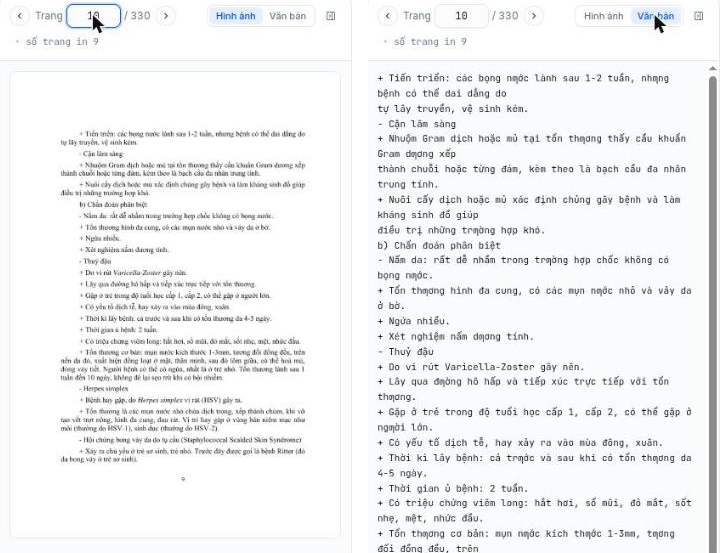
\includegraphics[width=0.8\linewidth,height=0.7\textheight,keepaspectratio]{chuong4/hinh/doc-noi-dung.png}
\caption{Kết quả đọc nội dung của một trang}
\label{fig:ket-qua-doc-noi-dung}
\end{figure}

\begin{figure}[H]
\centering
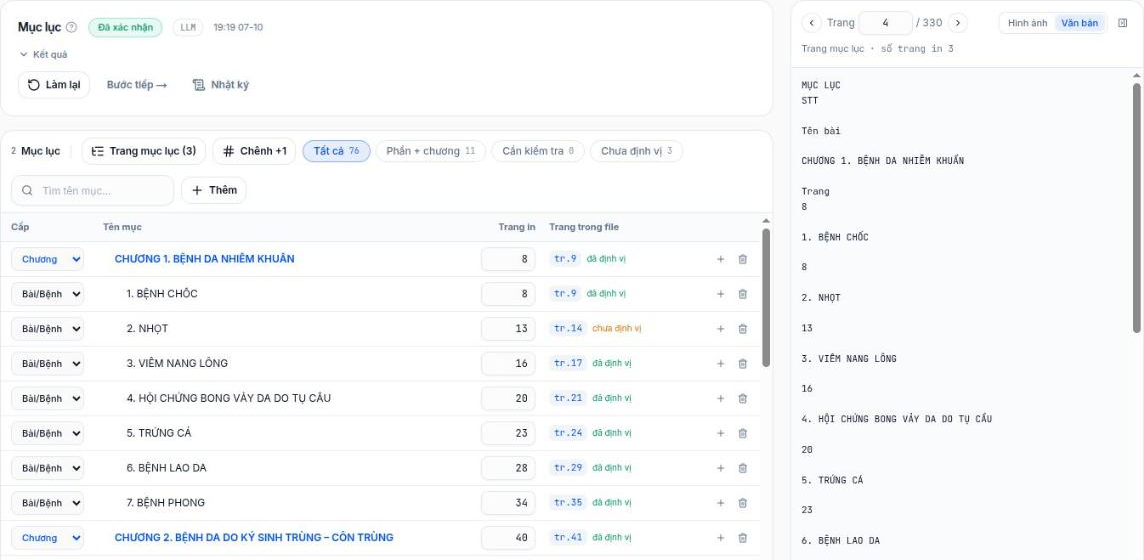
\includegraphics[width=0.95\linewidth,height=0.7\textheight,keepaspectratio]{chuong4/hinh/ket-qua-muc-luc.png}
\caption{Kết quả đọc mục lục của một sách}
\label{fig:ket-qua-muc-luc}
\end{figure}

\begin{figure}[H]
\centering
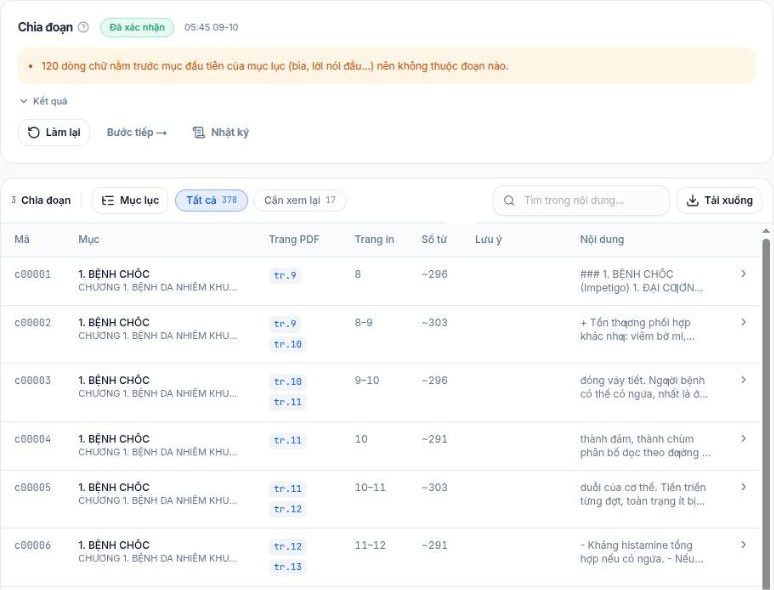
\includegraphics[width=0.9\linewidth,height=0.7\textheight,keepaspectratio]{chuong4/hinh/ket-qua-chia-doan.png}
\caption{Kết quả chia đoạn: chunk mẫu và danh sách cần soát}
\label{fig:ket-qua-chia-doan}
\end{figure}

\begin{figure}[H]
\centering

\includegraphics[width=0.9\linewidth,height=0.7\textheight,keepaspectratio]{chuong4/hinh/ket-qua-luu-kho.png}
\caption{Kết quả lưu vào kho tri thức: số đoạn đã lưu, số chiều vector, kho lưu trữ và mô hình tạo vector}
\label{fig:ket-qua-luu-kho}
\end{figure}

\begin{figure}[H]
\centering
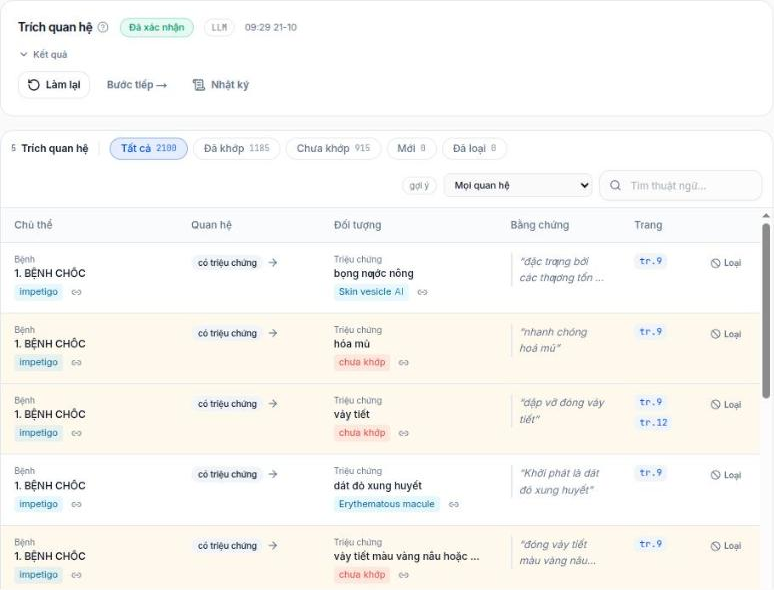
\includegraphics[width=0.9\linewidth,height=0.7\textheight,keepaspectratio]{chuong4/hinh/triple-browser.png}
\caption{Kết quả trích quan hệ: giao diện duyệt}
\label{fig:triple-browser}
\end{figure}

\textbf{Thông tin dữ liệu.}

Mỗi chunk là một point trong Qdrant, mang hai vector:
\begin{itemize}
  \item \textbf{Vector dense:} 4096 chiều, từ mô hình \texttt{qwen/qwen3-embedding-8b}, dùng cho tìm kiếm ngữ nghĩa.
  \item \textbf{Vector sparse:} tần suất từ theo BM25, dùng cho tìm kiếm từ khóa.
\end{itemize}

Thông tin đi kèm (payload) của point ghi \texttt{document\_id}, part, section, mục, số trang, mã các hình trong khoảng trang (\texttt{figure\_ids}) và đường dẫn file PDF gốc (\texttt{source\_pdf}).

\begin{table}[H]
\centering
\caption{Thống kê ba giáo trình đã nạp vào kho}
\label{tab:thong-ke-sach}
\small
\begin{tabular}{|p{5.2cm}|p{2.2cm}|p{1.6cm}|p{1.8cm}|p{2.4cm}|}
\hline
\textbf{Sách} & \textbf{Ngôn ngữ} & \textbf{Số trang} & \textbf{Số chunk} & \textbf{Số cạnh \texttt{DOC}} \\ \hline
Hướng dẫn chẩn đoán điều trị da liễu (Bộ Y tế) & Việt & 330 & 378 & 798 \\ \hline
Bệnh da liễu thường gặp (ĐH Y Dược TP.HCM) & Việt & 249 & 308 & 273 \\ \hline
Andrews' Diseases of the Skin & Anh & 1.083 & 4.232 & 7.731 \\ \hline
\end{tabular}
\end{table}

\begin{figure}[H]
\centering
\begin{tikzpicture}
\begin{axis}[
  xbar, width=0.8\linewidth, height=5cm, bar width=14pt,
  symbolic y coords={Andrews,{ĐH Y Dược TP.HCM},{Bộ Y tế}},
  ytick={Andrews,{ĐH Y Dược TP.HCM},{Bộ Y tế}}, y dir=reverse, enlarge y limits=0.3, xmin=0, xmax=5200,
  nodes near coords, nodes near coords align={horizontal},
  every node near coord/.append style={font=\small, text=black},
  /pgf/number format/.cd, fixed, set thousands separator={.}, precision=0,
  tick label style={font=\small}, xlabel={Số chunk}, xmajorgrids=true, grid style={gray!25},
  legend pos=south east, legend style={font=\small}, legend cell align=left]
\addplot[fill=blue!45!black!70, draw=none] coordinates {(308,{ĐH Y Dược TP.HCM}) (378,{Bộ Y tế})};
\addplot[fill=orange!70!black!75, draw=none] coordinates {(4232,Andrews)};
\legend{Tiếng Việt,Tiếng Anh}
\end{axis}
\end{tikzpicture}
\caption{Số chunk của ba giáo trình trong Qdrant}
\label{fig:chunk-theo-sach}
\end{figure}

Bước 6 đã nạp 8.802 cạnh từ ba sách (hình~\ref{fig:canh-doc-theo-sach}). Bước trích quan hệ cho ra 21.754 quan hệ, trong đó 10.267 quan hệ khớp đủ hai đầu vào PrimeKG hoặc DermO. Hệ thống bỏ 887 quan hệ có hai đầu trùng nút và gộp 578 quan hệ trùng cặp nút, còn 8.802 cạnh. Sách Fitzpatrick's Color Atlas mới qua bước chia đoạn (370 chunk), chưa lưu vào kho nên không nằm trong thống kê.

\begin{figure}[H]
\centering
\begin{tikzpicture}
\begin{axis}[
  xbar stacked, width=0.78\linewidth, height=7.6cm, bar width=9pt,
  symbolic y coords={DISEASE\_PHENOTYPE\_POSITIVE,INDICATION,ASSOCIATED\_WITH,IS\_A,DISEASE\_DISEASE,DISEASE\_PROTEIN,RESULTS\_IN,DISEASE\_PHENOTYPE\_NEGATIVE,DRUG\_EFFECT,EXPOSURE\_DISEASE,OFF\_LABEL\_USE,CONTRAINDICATION},
  ytick=data, y dir=reverse, enlarge y limits=0.06, xmin=0, xmax=4300,
  tick label style={font=\scriptsize}, xlabel={Số cạnh \texttt{DOC}}, xmajorgrids=true, grid style={gray!25},
  legend style={at={(0.97,0.5)}, anchor=east, font=\scriptsize}, legend cell align=left]
\addplot[fill=orange!70!black!75, draw=none] coordinates {(354,DISEASE\_PHENOTYPE\_POSITIVE) (198,INDICATION) (19,ASSOCIATED\_WITH) (78,IS\_A) (58,DISEASE\_DISEASE) (11,DISEASE\_PROTEIN) (18,RESULTS\_IN) (27,DISEASE\_PHENOTYPE\_NEGATIVE) (17,DRUG\_EFFECT) (11,EXPOSURE\_DISEASE) (1,OFF\_LABEL\_USE) (6,CONTRAINDICATION)};
\addplot[fill=teal!60!black!75, draw=none] coordinates {(93,DISEASE\_PHENOTYPE\_POSITIVE) (74,INDICATION) (15,ASSOCIATED\_WITH) (34,IS\_A) (23,DISEASE\_DISEASE) (10,DISEASE\_PROTEIN) (7,RESULTS\_IN) (4,DISEASE\_PHENOTYPE\_NEGATIVE) (10,DRUG\_EFFECT) (3,EXPOSURE\_DISEASE) (0,OFF\_LABEL\_USE) (0,CONTRAINDICATION)};
\addplot[fill=blue!45!black!70, draw=none] coordinates {(3565,DISEASE\_PHENOTYPE\_POSITIVE) (1415,INDICATION) (892,ASSOCIATED\_WITH) (530,IS\_A) (390,DISEASE\_DISEASE) (354,DISEASE\_PROTEIN) (226,RESULTS\_IN) (128,DISEASE\_PHENOTYPE\_NEGATIVE) (126,DRUG\_EFFECT) (74,EXPOSURE\_DISEASE) (24,OFF\_LABEL\_USE) (7,CONTRAINDICATION)};
\legend{Bộ Y tế,ĐH Y Dược TP.HCM,Andrews}
\end{axis}
\end{tikzpicture}
\caption{Số cạnh trích từ giáo trình theo loại quan hệ và theo sách (tổng 8.802 cạnh, ba sách)}
\label{fig:canh-doc-theo-sach}
\end{figure}

Hai loại quan hệ chiếm nhiều nhất là \texttt{DISEASE\_PHENOTYPE\_POSITIVE} (4.012 cạnh) và \texttt{INDICATION} (1.687 cạnh); hai loại này phục vụ các câu hỏi về triệu chứng và điều trị của bệnh.

\subsection{Ca bệnh đã kết luận của bác sĩ}

\subsubsection{Nội dung và vai trò của ca bệnh}

Ca bệnh đã kết luận là báo cáo kết luận do bác sĩ chốt khi đóng ca một phiên tư vấn. Mỗi phiên có một báo cáo và bác sĩ không sửa sau khi chốt. Chatbot dùng kho này để đối chiếu biểu hiện của người bệnh với các ca thực tế tương tự; kết quả chỉ để tham khảo, không phải chẩn đoán y khoa.

\subsubsection{Quy trình nạp ca bệnh vào Qdrant}

Hệ thống nạp ca vào một bộ lưu riêng trong Qdrant ngay sau khi bác sĩ lưu báo cáo kết luận.

\textbf{Bước 1. Tổng hợp văn bản.} Hệ thống đọc bản chụp (snapshot) của báo cáo lúc bác sĩ chốt và ghép thành một văn bản gồm chẩn đoán, thông tin bệnh nhân, dữ kiện lâm sàng, nhận định, dặn dò và thông tin ảnh, cùng thông tin đi kèm (payload), không chứa thông tin cá nhân (họ tên, số điện thoại).

\codeblock{chuong4/code/cb_van_ban}{Mã tổng hợp văn bản và payload của ca bệnh}{lst:cb-van-ban}

\textbf{Bước 2. Tạo vector và nạp point.} Hệ thống tính embedding dense và vector sparse BM25 (chế độ hỗn hợp Việt -- Anh) từ cùng văn bản, rồi ghi một point vào Qdrant.

\codeblock{chuong4/code/cb_nap_point}{Mã nạp một ca bệnh vào Qdrant}{lst:cb-nap-point}

\subsubsection{Kết quả nạp ca bệnh}

\textbf{Kết quả trực quan.}

\begin{figure}[H]
\centering
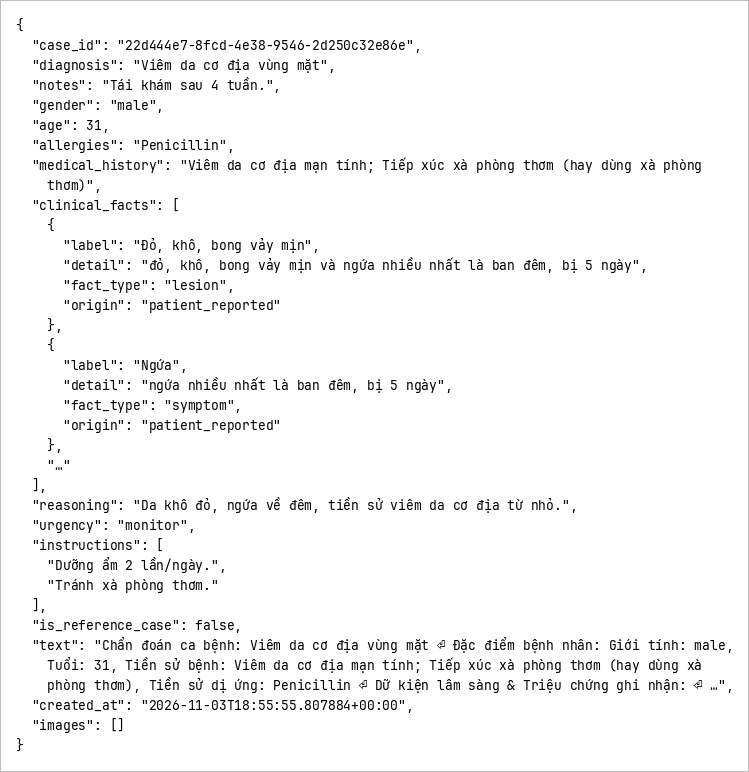
\includegraphics[width=0.75\linewidth,height=0.7\textheight,keepaspectratio]{chuong4/hinh/ca-benh-point.png}
\caption{Thông tin đi kèm của một ca bệnh trong Qdrant}
\label{fig:ca-benh-point}
\end{figure}

\textbf{Thông tin dữ liệu.} Mọi báo cáo đã chốt đều được nạp, kể cả ca chưa đánh dấu là ca tham khảo; dấu này hiện chỉ được ghi kèm, chưa dùng để lọc khi tra. Bảng~\ref{tab:cb-payload} liệt kê thông tin đi kèm mỗi point.

\begin{table}[H]
\centering
\caption{Thông tin đi kèm mỗi ca bệnh trong Qdrant}
\label{tab:cb-payload}
\small
\begin{tabular}{|p{4.0cm}|p{9.5cm}|}
\hline
\textbf{Trường} & \textbf{Ý nghĩa} \\ \hline
\texttt{case\_id} & Mã ca; mã point được sinh từ mã này \\ \hline
\texttt{diagnosis} & Chẩn đoán do bác sĩ chốt \\ \hline
\texttt{is\_reference\_case} & Dấu ca tham khảo do bác sĩ đặt \\ \hline
\texttt{created\_at} & Thời điểm tạo báo cáo \\ \hline
\texttt{gender} & Giới tính \\ \hline
\texttt{age} & Tuổi, tính từ năm sinh \\ \hline
\texttt{allergies} & Dị ứng \\ \hline
\texttt{medical\_history} & Tiền sử bệnh \\ \hline
\texttt{clinical\_facts} & Dữ kiện lâm sàng ghi nhận trong phiên \\ \hline
\texttt{reasoning} & Nhận định của bác sĩ \\ \hline
\texttt{urgency} & Mức khẩn cấp \\ \hline
\texttt{instructions} & Dặn dò và hướng xử trí \\ \hline
\texttt{notes} & Ghi chú bổ sung \\ \hline
\texttt{text} & Văn bản dùng để tạo vector \\ \hline
\texttt{images} & Ảnh gắn vào ca: nhãn đã xác nhận, vị trí, mô tả, tên và đường dẫn file \\ \hline
\end{tabular}
\end{table}

Hiện có 14 ca bệnh đã kết luận trong kho.

\subsection{Đồ thị tri thức có sẵn: PrimeKG và DermO}
\label{sec:do-thi-tri-thuc}

\subsubsection{Nội dung và vai trò của đồ thị}

Neo4j chứa đồ thị có sẵn gồm hai phần, cùng quan hệ trích từ giáo trình (mục~\ref{sec:giao-trinh}):
\begin{itemize}
  \item \textbf{PrimeKG:} đồ thị y sinh có sẵn. Hệ thống giữ 5 loại nút (bệnh, thuốc, phenotype, gen/protein, phơi nhiễm) và 11 loại quan hệ, khoảng 3,46 triệu cạnh.
  \item \textbf{DermO:} ontology da liễu, 3.427 thuật ngữ, mỗi thuật ngữ có từ đồng nghĩa và thuật ngữ cha. Dùng để chuẩn hóa tên, không dùng để suy ra quan hệ lâm sàng.
\end{itemize}

PrimeKG và DermO không có cạnh nối nhau; hệ thống nối chúng bằng so khớp tên lúc truy vấn.

\begin{figure}[H]
\centering
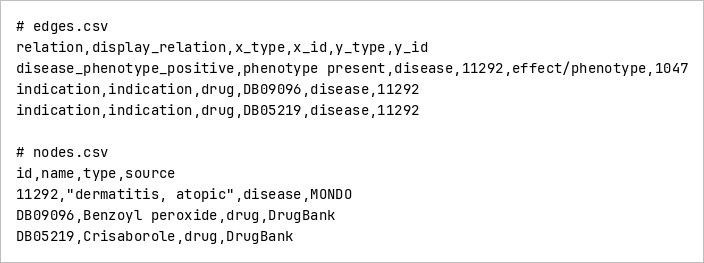
\includegraphics[width=0.85\linewidth,height=0.7\textheight,keepaspectratio]{chuong4/hinh/nguon-primekg.png}
\caption{Dữ liệu PrimeKG sau khi lọc: bảng cạnh và bảng nút}
\label{fig:nguon-primekg}
\end{figure}

\begin{figure}[H]
\centering
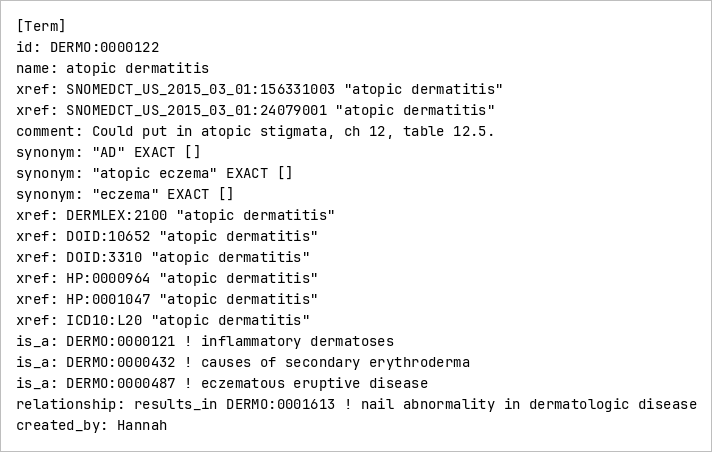
\includegraphics[width=0.85\linewidth,height=0.7\textheight,keepaspectratio]{chuong4/hinh/nguon-dermo.png}
\caption{Dữ liệu nguồn của DermO: một khối thuật ngữ}
\label{fig:nguon-dermo}
\end{figure}

\subsubsection{Quy trình nạp đồ thị vào Neo4j}

Hai phần có sẵn được dựng như sau.

\textbf{PrimeKG, bước 1. Lọc.} Nguồn là bảng quan hệ của PrimeKG (Harvard Dataverse, phiên bản 2). Hệ thống chỉ giữ 5 loại nút và 11 loại quan hệ trong phạm vi, bỏ dòng thiếu mã và cạnh trùng, rồi ghi danh sách nút và cạnh trung gian.

\codeblock{chuong4/code/dt_primekg_loc}{Mã lọc quan hệ PrimeKG}{lst:dt-primekg-loc}

\textbf{PrimeKG, bước 2. Nạp vào Neo4j.} Hệ thống nạp cạnh theo lô; quan hệ đã có cạnh được gộp (merge) để nạp lại không nhân đôi.

\codeblock{chuong4/code/dt_primekg_nap}{Mã nạp cạnh PrimeKG}{lst:dt-primekg-nap}

\textbf{DermO, bước 1. Đọc tệp ontology.} Tệp DermO (định dạng OBO, phiên bản 1.19) gồm các khối thuật ngữ; hệ thống đọc mỗi khối thành một thuật ngữ có tên, định nghĩa, từ đồng nghĩa, thuật ngữ cha và các quan hệ.

\codeblock{chuong4/code/dt_dermo_doc}{Mã đọc tệp ontology DermO}{lst:dt-dermo-doc}

\textbf{DermO, bước 2. Nạp vào Neo4j.} Mỗi thuật ngữ thành một nút \texttt{DermoTerm}. Quan hệ ``là một'' (\texttt{is\_a}) thành cạnh \texttt{IS\_A}; các quan hệ khác giữ tên gốc viết hoa (ví dụ \texttt{HAS\_SYMPTOM}, \texttt{RESULTS\_IN}).

\codeblock{chuong4/code/dt_dermo_nap}{Mã nạp cạnh DermO}{lst:dt-dermo-nap}

\subsubsection{Kết quả nạp đồ thị}

\textbf{Kết quả trực quan.}

Hình~\ref{fig:schema-neo4j} là lược đồ (schema) của đồ thị tri thức, lấy từ Neo4j Browser bằng \texttt{db.schema.visualization()}, gồm năm loại nút của PrimeKG và nút \texttt{DermoTerm} của DermO. Hình đã lọc bỏ các nhãn của đồ thị hành trình bệnh nhân. Mỗi vòng tự nối là một loại quan hệ giữa hai nút cùng loại; các quan hệ nối \texttt{DermoTerm} (\texttt{IS\_A}, \texttt{HAS\_SYMPTOM}, \ldots) gồm cả cạnh trích từ giáo trình.

\begin{figure}[H]
\centering
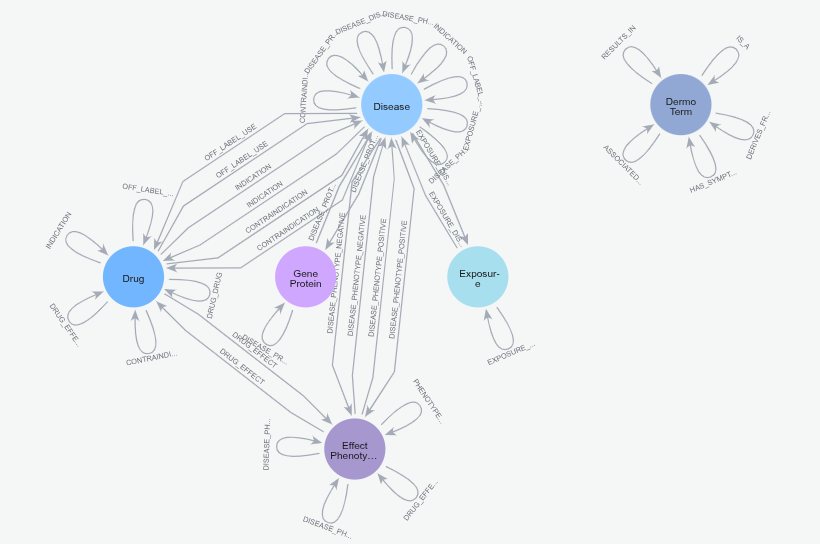
\includegraphics[width=0.95\linewidth,height=0.6\textheight,keepaspectratio]{chuong4/hinh/schema-neo4j.png}
\caption{Lược đồ đồ thị tri thức trong Neo4j Browser (sáu loại nút, không gồm đồ thị hành trình bệnh nhân)}
\label{fig:schema-neo4j}
\end{figure}

\begin{figure}[H]
\centering
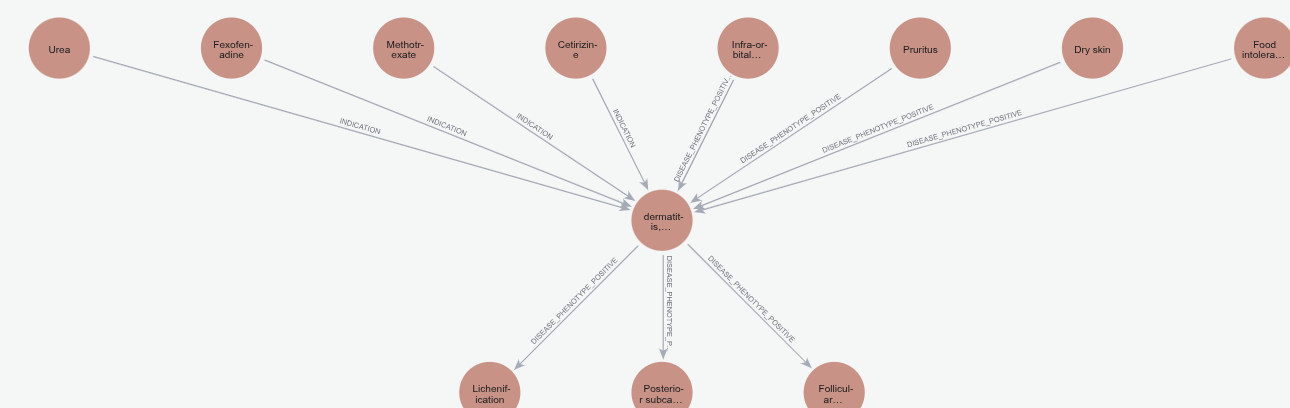
\includegraphics[width=\linewidth,keepaspectratio]{chuong4/hinh/do-thi-mau.png}
\caption{Đồ thị quanh bệnh \textit{dermatitis, atopic} trong Neo4j Browser: thuốc chỉ định (cạnh \texttt{INDICATION}) và triệu chứng, dấu hiệu lâm sàng của bệnh (cạnh \texttt{DISEASE\_PHENOTYPE\_POSITIVE})}
\label{fig:do-thi-mau}
\end{figure}

\begin{figure}[H]
\centering
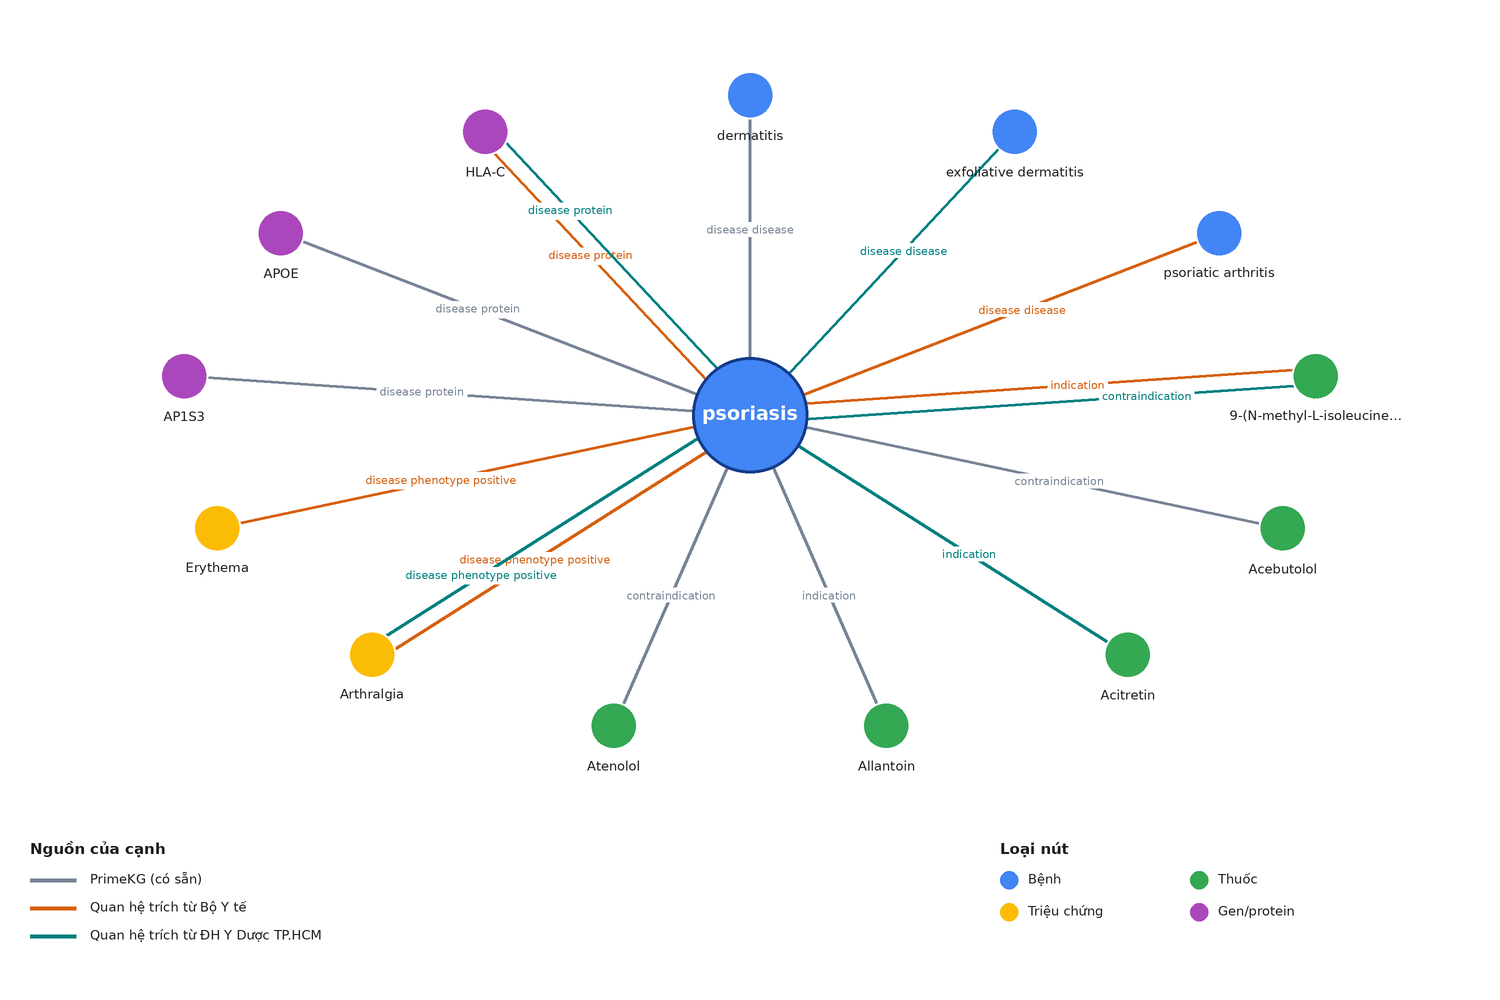
\includegraphics[width=0.95\linewidth,height=0.7\textheight,keepaspectratio]{chuong4/hinh/so-sanh-nguon-canh.png}
\caption{Cạnh PrimeKG và cạnh trích từ hai giáo trình quanh bệnh psoriasis}
\label{fig:so-sanh-nguon-canh}
\end{figure}


\textbf{Thông tin dữ liệu.}

Hình~\ref{fig:primekg-nut} và~\ref{fig:primekg-canh} thống kê PrimeKG đã nạp. Loại cạnh \texttt{DRUG\_DRUG} chiếm khoảng 77\% tổng số cạnh nên trục số cạnh dùng thang logarit. Các truy vấn của chatbot không duyệt loại cạnh này.

\begin{figure}[H]
\centering
\begin{tikzpicture}
\begin{axis}[
  xbar, width=0.85\linewidth, height=5.2cm, bar width=12pt,
  symbolic y coords={Phơi nhiễm,Thuốc,Gen/protein,Phenotype,Bệnh}, ytick=data,
  xmin=0, xmax=21000, enlarge y limits=0.15, scaled x ticks=false, xtick={0,5000,10000,15000,20000},
  nodes near coords, nodes near coords align={horizontal},
  every node near coord/.append style={font=\small, text=black},
  /pgf/number format/.cd, fixed, set thousands separator={.}, precision=0,
  xlabel={Số nút}, tick label style={font=\small}, xmajorgrids=true, grid style={gray!25},
  ]
\addplot[fill=blue!45!black!70, draw=none] coordinates {(474,Phơi nhiễm) (4540,Thuốc) (9080,Gen/protein) (15310,Phenotype) (17080,Bệnh)};
\end{axis}
\end{tikzpicture}
\caption{Số nút của PrimeKG theo loại (bệnh gồm cả nhóm \texttt{MONDO\_grouped})}
\label{fig:primekg-nut}
\end{figure}

\begin{figure}[H]
\centering
\begin{tikzpicture}
\begin{axis}[
  xbar, width=0.78\linewidth, height=8.6cm, bar width=9pt, xmode=log, log origin=infty,
  xmin=1000, xmax=60000000,
  symbolic y coords={DISEASE\_PHENOTYPE\_NEGATIVE,EXPOSURE\_DISEASE,OFF\_LABEL\_USE,INDICATION,PHENOTYPE\_PHENOTYPE,CONTRAINDICATION,DISEASE\_DISEASE,DRUG\_EFFECT,DISEASE\_PROTEIN,DISEASE\_PHENOTYPE\_POSITIVE,DRUG\_DRUG},
  ytick=data, y dir=reverse, enlarge y limits=0.06,
  nodes near coords,
  every node near coord/.append style={font=\scriptsize, text=black, anchor=west, xshift=2pt, yshift=0pt}, point meta=explicit symbolic,
  /pgf/number format/.cd, fixed, set thousands separator={.}, precision=0,
  xlabel={Số cạnh (thang logarit)}, tick label style={font=\scriptsize}, xmajorgrids=true, grid style={gray!25},
  ]
\addplot[fill=teal!60!black!75, draw=none] coordinates {(2672628,DRUG\_DRUG) [2.672.628] (300634,DISEASE\_PHENOTYPE\_POSITIVE) [300.634] (160822,DISEASE\_PROTEIN) [160.822] (129568,DRUG\_EFFECT) [129.568] (64388,DISEASE\_DISEASE) [64.388] (61350,CONTRAINDICATION) [61.350] (37472,PHENOTYPE\_PHENOTYPE) [37.472] (18776,INDICATION) [18.776] (5136,OFF\_LABEL\_USE) [5.136] (4608,EXPOSURE\_DISEASE) [4.608] (2386,DISEASE\_PHENOTYPE\_NEGATIVE) [2.386]};
\end{axis}
\end{tikzpicture}
\caption{Số cạnh của PrimeKG theo loại quan hệ}
\label{fig:primekg-canh}
\end{figure}


\section{Các luồng truy xuất tri thức của chatbot}
\label{sec:luong-truy-xuat}

\subsection{Truy xuất trong luồng RAG của chatbot}
\label{sec:rag-tong-quan}

Truy xuất tăng cường sinh văn bản (RAG) gồm hai phần: tìm bằng chứng trong kho tri thức, rồi để mô hình ngôn ngữ sinh câu trả lời dựa trên bằng chứng đó. Chatbot thực hiện bốn bước:
\begin{enumerate}
  \item \textbf{Nạp tri thức:} giáo trình được cắt thành đoạn và nạp vào Qdrant; quan hệ trích từ sách nạp vào Neo4j; ca bệnh nạp vào kho riêng (mục~\ref{sec:nguon-kb}).
  \item \textbf{Truy xuất:} agent gọi công cụ tra cứu, công cụ chạy ba hướng tìm kiếm ngữ nghĩa, từ khóa, đồ thị và gộp kết quả bằng RRF (các mục từ~\ref{sec:luong-ngu-nghia} đến~\ref{sec:luong-hon-hop}).
  \item \textbf{Đưa bằng chứng vào ngữ cảnh:} mỗi kết quả nhận một mã \texttt{E\#} kèm sách, mục và số trang (Chương~\ref{ch:chuong5}).
  \item \textbf{Sinh câu trả lời:} agent chỉ giữ giả thuyết có ít nhất một mã \texttt{E\#} hợp lệ; câu trả lời là gợi ý hỗ trợ, không phải chẩn đoán y khoa (Chương~\ref{ch:chuong5}).
\end{enumerate}
Chương này mô tả hai bước đầu. Hai bước sau thuộc luồng lập luận của agent ở Chương~\ref{ch:chuong5}.

\subsection{Các luồng truy xuất trên văn bản giáo trình}

Trên các đoạn giáo trình (chunk), hệ thống có ba hướng tìm kiếm. Hai hướng đầu, ngữ nghĩa và từ khóa, bổ sung cho nhau. Hướng thứ ba đi qua đồ thị: từ thực thể trong câu hỏi tới quan hệ đã trích từ sách, rồi tới các đoạn chứa câu trích của quan hệ đó (bảng~\ref{tab:bu-dap}). Ca bệnh đã kết luận dùng hai hướng đầu trên kho riêng; hướng đồ thị chỉ áp dụng cho giáo trình.

\begin{table}[H]
\centering
\caption{Ba hướng tìm kiếm bổ sung cho nhau}
\label{tab:bu-dap}
\small
\begin{tabular}{|p{2.0cm}|p{3.8cm}|p{3.8cm}|p{3.9cm}|}
\hline
\textbf{Tiêu chí} & \textbf{Ngữ nghĩa (dense)} & \textbf{Từ khóa (BM25, sparse)} & \textbf{Đồ thị (liên kết tới đoạn)} \\ \hline
So khớp & Cosine giữa vector câu hỏi và vector đoạn & Từ trùng, có trọng số theo độ hiếm & Tên thực thể trùng tên hoặc từ đồng nghĩa của nút; lấy đoạn gắn với quan hệ của nút \\ \hline
Bắt được & Diễn đạt khác nghĩa cùng; câu hỏi tiếng Việt, sách tiếng Anh & Tên thuốc, hoạt chất, mã bệnh, liều & Đoạn mà sách đã trích thành quan hệ với thực thể được hỏi, kể cả khi đoạn dùng từ khác \\ \hline
Bỏ sót & Token hiếm bị làm mờ trong vector & Câu hỏi và đoạn không có từ chung & Thực thể chưa có quan hệ trích từ sách; không đi qua nút lân cận \\ \hline
\end{tabular}
\end{table}

Ví dụ: câu hỏi ``da tôi đỏ và ngứa, nổi thành mảng'' và đoạn chứa ``erythematous pruritic plaques'' không có từ chung. BM25 cho điểm $0$, tìm kiếm ngữ nghĩa vẫn khớp. Ngược lại, câu hỏi về một tên thuốc cụ thể được BM25 khớp đúng chữ, trong khi vector có thể gộp thuốc đó với các thuốc cùng nhóm.


Mã nguồn đặc trưng của từng luồng được trích ở các mã nguồn~\ref{lst:ngu-nghia}, \ref{lst:bm25}, \ref{lst:graph-leg}, \ref{lst:rrf}, \ref{lst:hybrid} và~\ref{lst:seed}. Phần sau mô tả từng luồng đơn (mục~\ref{sec:luong-ngu-nghia}, \ref{sec:luong-tu-khoa} và~\ref{sec:luong-do-thi}), rồi luồng hỗn hợp ghép ba luồng đó (mục~\ref{sec:luong-hon-hop}).

\subsection{Luồng tìm kiếm ngữ nghĩa}
\label{sec:luong-ngu-nghia}

\subsubsection{Nguyên lý tìm kiếm ngữ nghĩa}

Tìm kiếm ngữ nghĩa so khớp theo nghĩa của câu thay vì theo ký tự. Mô hình embedding đổi mỗi đoạn văn bản thành một vector thực $d$ chiều. Bài toán tra cứu trở thành bài toán hình học: tìm các vector đoạn gần vector câu hỏi nhất.

Hệ thống dùng mô hình \texttt{qwen/qwen3-embedding-8b} (8 tỷ tham số), đầu ra $d=4096$ chiều. Mô hình có hai đặc tính:
\begin{itemize}
  \item \textbf{Instruction-tuned:} câu hỏi được thêm tiền tố chỉ dẫn; đoạn trong kho tri thức được mã hóa ở dạng nguyên bản.
  \item \textbf{Đa ngôn ngữ:} câu hỏi tiếng Việt và đoạn tiếng Anh nằm chung một không gian vector.
\end{itemize}

\subsubsection{Cơ chế tìm kiếm ngữ nghĩa}

Gọi $f$ là hàm embedding. Quy trình có hai giai đoạn:
\begin{itemize}
  \item \textbf{Nạp dữ liệu (indexing):} mỗi đoạn được mã hóa một lần, $d=f(\text{đoạn})$, rồi lưu vào Qdrant.
  \item \textbf{Truy vấn (querying):} câu hỏi được mã hóa một lần, $q=f(\text{câu hỏi})$. Kiến trúc Bi-Encoder mã hóa câu hỏi và đoạn độc lập, nên vector đoạn được tính trước và độ trễ lúc truy vấn thấp.
\end{itemize}

Độ liên quan giữa $q$ và $d$ là độ tương đồng cosine:
\begin{equation}
  \mathrm{sim}(q,d)=\frac{q\cdot d}{\Vert q\Vert \Vert d\Vert }
\end{equation}

Trong đó, $\mathrm{sim}(q,d)\in[-1,1]$. Phép đo chỉ phụ thuộc hướng vector nên không bị lệch bởi độ dài đoạn.

Hệ thống xếp các đoạn theo $\mathrm{sim}$ giảm dần, lấy $k$ đoạn đầu, đọc nội dung và siêu dữ liệu (sách, mục, trang) theo ID vector rồi trả về.

\codeblock{chuong4/code/dense}{Mã tìm kiếm ngữ nghĩa: mã hóa câu hỏi (có tiền tố chỉ dẫn) và truy vấn Qdrant}{lst:ngu-nghia}

\subsection{Luồng tìm kiếm từ khóa}
\label{sec:luong-tu-khoa}

\subsubsection{Nguyên lý tìm kiếm từ khóa}

Tìm kiếm từ khóa khớp chính xác chuỗi ký tự. Luồng này bù cho điểm yếu của vector: tên thuốc, hoạt chất, mã bệnh và liều lượng thường bị làm mờ trong embedding.

\textbf{TF-IDF} là nền tảng của phương pháp. Điểm của tài liệu $D$ với câu hỏi $Q$ là tổng, trên các từ $t\in Q$, của tích tần suất từ trong tài liệu ($\mathrm{tf}$) và độ hiếm của từ trong kho ($\mathrm{idf}$):
\begin{equation}
  \mathrm{score}_{\mathrm{TF\text{-}IDF}}(D,Q)=\sum _{t\in Q} \mathrm{tf}(t,D)\cdot \mathrm{idf}(t)
\end{equation}
Hai thành phần được tính như sau:
\begin{equation}
  \mathrm{tf}(t,D)=f(t,D)
\end{equation}
\begin{equation}
  \mathrm{idf}(t)=\ln\frac{N}{n(t)}
\end{equation}
Trong đó $f(t,D)$ là số lần từ $t$ xuất hiện trong đoạn $D$, $N$ là tổng số đoạn trong kho và $n(t)$ là số đoạn chứa $t$. Từ xuất hiện trong ít đoạn có $\mathrm{idf}$ lớn nên đóng góp nhiều vào điểm. Từ có mặt ở mọi đoạn ($n(t)=N$) có $\mathrm{idf}=0$ và không ảnh hưởng đến điểm.

TF-IDF có hai hạn chế:
\begin{itemize}
  \item \textbf{Không bão hòa:} điểm tăng tuyến tính theo tần suất từ, dù từ lặp lại nhiều lần không làm đoạn liên quan hơn tương ứng.
  \item \textbf{Không chuẩn hóa độ dài:} đoạn dài chứa nhiều từ hơn nên được điểm cao hơn.
\end{itemize}

\subsubsection{Thuật toán xếp hạng BM25}

BM25 (Best Matching 25) thêm hai tham số để sửa hai hạn chế trên:
\begin{equation}
  \mathrm{score}(D,Q)=\sum_{t\in Q}\mathrm{IDF}(t)\cdot\frac{\mathrm{tf}\cdot(k_1+1)}{\mathrm{tf}+k_1\cdot\left(1-b+b\cdot\frac{|D|}{\mathrm{avgdl}}\right)}
\end{equation}
\begin{equation}
  \mathrm{IDF}(t)=\ln\left( 1+\frac{N-n(t)+0{,}5}{n(t)+0{,}5}\right)
\end{equation}

Trong đó:
\begin{itemize}
  \item $\mathrm{tf}(t,D)$: số lần từ $t$ xuất hiện trong $D$; $n(t)$: số đoạn chứa $t$; $N$: tổng số đoạn.
  \item $k_1=1{,}2$: giới hạn mức tăng điểm theo tần suất từ (độ bão hòa).
  \item $b=0{,}75$: mức chuẩn hóa theo tỷ số giữa độ dài đoạn $|D|$ và độ dài trung bình $\mathrm{avgdl}$.
\end{itemize}

Qdrant lưu phần $\mathrm{tf}$ của mỗi đoạn dưới dạng vector thưa (sparse) và chấm điểm khi truy vấn. Cấu trúc này hoạt động như chỉ mục đảo: mỗi từ trỏ tới các đoạn chứa nó, nên truy vấn không phải duyệt toàn bộ kho.

\subsubsection{Cơ chế tìm kiếm từ khóa}

\begin{itemize}
  \item \textbf{Mở rộng câu hỏi Việt -- Anh:} LLM trích thực thể y khoa từ câu hỏi và thêm tên tiếng Anh, tiếng Việt vào câu hỏi BM25, để khớp với sách viết khác ngôn ngữ câu hỏi. Khi LLM lỗi, BM25 dùng câu hỏi gốc và hệ thống ghi chú lại.
  \item \textbf{Tiền xử lý tiếng Việt:} tách từ ghép bằng underthesea, loại stopword nhưng giữ từ phủ định và đơn vị liều. Thêm token bỏ dấu với trọng số thấp ($0{,}3$) để câu hỏi không dấu vẫn khớp.
  \item \textbf{Cách dùng:} chạy độc lập khi cần tra tên chính xác, và là một nhánh của luồng hỗn hợp.
\end{itemize}

\codeblock{chuong4/code/sparse}{Mã chuyển văn bản thành vector thưa BM25: \texttt{encode\_document} lưu vào Qdrant, \texttt{encode\_query} dùng khi truy vấn}{lst:bm25}

\subsection{Luồng tìm kiếm đồ thị}
\label{sec:luong-do-thi}

\subsubsection{Nguyên lý tìm kiếm đồ thị}

Hai luồng trước so khớp câu hỏi với nội dung đoạn. Luồng đồ thị so khớp theo thực thể y khoa và đi ngược từ thực thể về đoạn. Quan hệ trích từ sách (mục~\ref{sec:giao-trinh}) lưu mã các đoạn chứa câu trích, nên từ một thực thể có thể lấy lại các đoạn đó, kể cả khi đoạn dùng từ khác với câu hỏi.

Điểm của đoạn $c$ là số quan hệ trỏ tới nó:
\begin{equation}
  \mathrm{score}_{G}(c)=\bigl|\{\,r\in R(E)\;:\;c\in \mathrm{chunks}(r)\,\}\bigr|
\end{equation}

Trong đó $E$ là tập nút đồ thị khớp với thực thể trong câu hỏi, $R(E)$ là tập quan hệ trích từ sách nối trực tiếp với một nút thuộc $E$, và $\mathrm{chunks}(r)$ là tập đoạn chứa câu trích của quan hệ $r$. Đoạn cùng điểm được xếp theo mã đoạn.

Luồng này trả về đoạn giáo trình. Việc truy vấn đồ thị để chọn bệnh ứng viên là chức năng khác, trình bày ở mục~\ref{sec:truy-xuat-do-thi}.

\subsubsection{Cơ chế tìm kiếm đồ thị}

Luồng chỉ chạy với kho giáo trình; với kho ca bệnh, luồng trả danh sách rỗng.
\begin{enumerate}
  \item \textbf{Lấy tên thực thể:} tên tiếng Anh và tiếng Việt của các thực thể y khoa trong câu hỏi, bỏ loại khác.
  \item \textbf{Tìm nút:} tối đa 10 nút của đồ thị có tên hoặc từ đồng nghĩa khớp, không phân biệt hoa thường. Hệ thống khớp chính xác trước, chỉ khi không có kết quả mới khớp theo chuỗi con.
  \item \textbf{Lấy đoạn từ quan hệ:} các quan hệ trích từ sách nối trực tiếp với những nút đó (một bước, không phân biệt hướng); mỗi quan hệ cho các đoạn chứa câu trích của nó.
  \item \textbf{Xếp hạng và lấy đoạn:} đoạn có nhiều quan hệ trỏ tới xếp trước, rồi lấy nội dung đoạn từ Qdrant.
\end{enumerate}

\codeblock{chuong4/code/graph_leg}{Mã luồng đồ thị: từ thực thể tới đoạn giáo trình}{lst:graph-leg}

Đoạn do luồng này đề xuất được gắn dấu để chatbot biết nguồn là đồ thị. Phạm vi của luồng hẹp: chỉ xét quan hệ nối trực tiếp với thực thể và chỉ dùng quan hệ trích từ sách, vì quan hệ của hai đồ thị có sẵn không gắn với đoạn nào. Luồng trả rỗng khi sách chưa trích quan hệ hoặc khi đoạn đã chia lại mà chưa trích lại; lúc đó luồng hỗn hợp chạy với hai nhánh còn lại.

\subsection{Luồng hỗn hợp (\texttt{hybrid\_retrieval})}
\label{sec:luong-hon-hop}

\subsubsection{Quy trình truy xuất hỗn hợp}

Luồng hỗn hợp ghép ba luồng ở trên theo bốn bước (hình~\ref{fig:hybrid}). Mục tiêu của hai bước đầu là không bỏ sót đoạn liên quan (recall). Mục tiêu của hai bước sau là đưa đoạn đúng lên đầu (precision).
\begin{enumerate}
  \item \textbf{Chuẩn bị câu hỏi:} trích thực thể y khoa; thực thể dùng để mở rộng câu hỏi cho nhánh BM25 và làm đầu vào cho nhánh đồ thị.
  \item \textbf{Ba nhánh song song:} nhánh ngữ nghĩa, nhánh BM25 và nhánh đồ thị, mỗi nhánh lấy tối đa 20 đoạn.
  \item \textbf{Gộp bằng RRF,} khử trùng theo ID đoạn, giữ 20 đoạn đầu.
  \item \textbf{Xếp hạng lại} bằng Cross-Encoder, trả về $k$ đoạn đầu kèm sách, mục, số trang.
\end{enumerate}

Khi một nhánh lỗi, công cụ dùng kết quả của các nhánh còn lại. Khi reranker không dùng được, công cụ giữ thứ tự sau RRF. Cả hai trường hợp đều được ghi chú trong kết quả trả về để chatbot báo rõ nguồn nào chưa tra được.

\begin{figure}[H]
\centering
\begin{tikzpicture}[
  font=\small, >=Stealth,
  box/.style={rectangle, rounded corners=3pt, draw=gray!70, fill=gray!12, minimum width=3.2cm, minimum height=0.9cm, align=center},
  leg/.style={rectangle, rounded corners=3pt, draw=blue!55!black, fill=blue!10, text width=3.9cm, minimum height=1.4cm, align=center, inner sep=3pt},
  fuse/.style={rectangle, rounded corners=3pt, draw=orange!70!black, fill=orange!12, minimum width=3.4cm, minimum height=0.9cm, align=center},
  lab/.style={font=\scriptsize, midway, right}]
\node[box] (q) at (0,0) {Câu hỏi};
\node[box] (ent) at (0,-1.7) {Trích thực thể y khoa};
\node[leg] (sem) at (-4.9,-4) {Nhánh ngữ nghĩa\\(vector dense)\\{\scriptsize tối đa 20 đoạn}};
\node[leg] (bm) at (0,-4) {Nhánh từ khóa\\(BM25, câu hỏi mở rộng)\\{\scriptsize tối đa 20 đoạn}};
\node[leg] (gr) at (4.9,-4) {Nhánh đồ thị\\(thực thể $\rightarrow$ quan hệ $\rightarrow$ đoạn)\\{\scriptsize tối đa 20 đoạn}};
\node[fuse] (rrf) at (0,-6.6) {Gộp bằng RRF\\(giữ 20 đoạn)};
\node[fuse] (re) at (0,-8.3) {Xếp hạng lại\\(Cross-Encoder)};
\node[box] (out) at (0,-10) {$k$ đoạn kèm sách, mục, số trang};
\draw[->] (q) -- (ent);
\draw[->] (q.west) -| (sem.north);
\draw[->] (ent) -- (bm);
\draw[->] (ent.east) -| (gr.north);
\draw[->] (sem.south) |- (rrf.west);
\draw[->] (bm) -- (rrf);
\draw[->] (gr.south) |- (rrf.east);
\draw[->] (rrf) -- (re);
\draw[->] (re) -- (out);
\end{tikzpicture}
\caption{Luồng truy xuất hỗn hợp}
\label{fig:hybrid}
\end{figure}

\subsubsection{Gộp kết quả bằng RRF}

RRF (Reciprocal Rank Fusion) gộp theo thứ hạng thay vì điểm thô, vì điểm cosine và điểm BM25 có thang khác nhau, còn nhánh đồ thị chỉ có thứ hạng theo số quan hệ:
\begin{equation}
  \mathrm{RRF}(d)=\sum_{i\in \mathrm{lists}} \frac{1}{k+\mathrm{rank}_{i}(d)},\quad k=60
\end{equation}

Trong đó $\mathrm{rank}_i(d)$ là thứ hạng của đoạn $d$ trong danh sách $i$. Đoạn xuất hiện ở nhiều danh sách được cộng nhiều số hạng nên lên cao. Hằng số $k=60$ làm giảm chênh lệch giữa các vị trí đầu, nên không nhánh nào chi phối hoàn toàn. Hệ thống không dùng chuẩn hóa điểm có trọng số $\alpha$ vì phương pháp này nhạy với giá trị ngoại lai trong từng truy vấn và cần chỉnh $\alpha$ bằng thực nghiệm, trong khi chưa có tập đánh giá đủ lớn.

\codeblock{chuong4/code/rrf}{Mã gộp kết quả ba nhánh bằng RRF}{lst:rrf}

\subsubsection{Xếp hạng lại bằng Cross-Encoder}

Mô hình \texttt{qwen/qwen3-reranker-8b} nhận từng cặp $(\text{câu hỏi},\text{đoạn})$ và cho điểm từ $0$ đến $1$. Khác Bi-Encoder, Cross-Encoder đọc câu hỏi và đoạn cùng lúc nên đánh giá được tương tác giữa hai chuỗi, nhưng chậm hơn. Vì vậy mô hình chỉ chạy trên 20 đoạn sau RRF.

\codeblock{chuong4/code/hybrid}{Mã điều phối luồng hỗn hợp}{lst:hybrid}

\subsubsection{Đánh giá luồng hỗn hợp}

Bộ kiểm thử lấy từ 378 chunk của sách Bộ Y tế; hai sách còn lại (cùng 4.540 chunk) chưa nằm trong bộ kiểm thử. RAGAS sinh câu hỏi theo vai bệnh nhân từ 120 chunk hợp lệ (loại chunk ngắn hơn 300 ký tự, mục lục, phụ lục), kết quả 24 câu (10 đơn bước, 14 đa bước) và 36 nhãn chunk.

\begin{table}[H]
\centering
\caption{Kết quả đánh giá các luồng truy xuất trên bộ kiểm thử (n = 24)}
\label{tab:ket-qua-truy-xuat}
\small
\begin{tabular}{|l|c|c|c|c|c|c|}
\hline
\textbf{Luồng truy xuất} & \textbf{hit@1} & \textbf{hit@3} & \textbf{hit@5} & \textbf{hit@10} & \textbf{recall@10} & \textbf{MRR@10} \\ \hline
Ngữ nghĩa & 0,58 & 0,75 & 0,83 & 0,96 & 0,90 & 0,70 \\ \hline
Từ khóa BM25 & 0,50 & 0,67 & 0,83 & 0,88 & 0,73 & 0,63 \\ \hline
\textbf{Hỗn hợp} & \textbf{0,83} & \textbf{0,92} & \textbf{1,00} & \textbf{1,00} & \textbf{0,94} & \textbf{0,90} \\ \hline
\end{tabular}
\end{table}

Luồng hỗn hợp cao nhất ở mọi chỉ số. So với luồng ngữ nghĩa, hit@5 tăng $0{,}17$ (khoảng tin cậy 95\% $[0{,}04;\,0{,}33]$). Rerank nâng hit@1 từ $0{,}67$ (sau RRF) lên $0{,}83$.

Bộ kiểm thử có các hạn chế:
\begin{itemize}
  \item Cỡ mẫu nhỏ nên khoảng tin cậy rộng.
  \item Câu hỏi sinh từ chính chunk nên văn phong gần văn bản gốc, thiên lợi cho BM25.
  \item Chưa kiểm tra thủ công toàn bộ nhãn.
  \item Bộ kiểm thử chỉ dùng sách tiếng Việt, chưa dùng sách Andrews (tiếng Anh) nên chưa đo được truy vấn xuyên ngôn ngữ.
  \item Bảng~\ref{tab:ket-qua-truy-xuat} chỉ gồm nhánh ngữ nghĩa và BM25. % TODO: đo lại luồng hỗn hợp sau khi thêm nhánh đồ thị
  \item Chưa đánh giá kho ca bệnh và truy xuất đồ thị.
\end{itemize}

\subsection{Truy xuất trực tiếp trên PrimeKG và DermO}
\label{sec:truy-xuat-do-thi}

Ngoài luồng đồ thị đi về đoạn giáo trình (mục~\ref{sec:luong-do-thi}), chatbot truy vấn trực tiếp đồ thị có sẵn (PrimeKG, DermO) để lấy quan hệ y khoa và bệnh ứng viên.

\subsubsection{Giải quyết thực thể}

Chatbot nêu tên thực thể (tối đa 6) khi truy vấn. Hệ thống ánh xạ các tên này về nút đồ thị:
\begin{enumerate}
  \item Tra DermO (khớp tên hoặc từ đồng nghĩa) để lấy tên chuẩn.
  \item Dùng tập tên chuẩn khớp nút PrimeKG loại bệnh, triệu chứng hoặc thuốc. Hệ thống khớp chính xác trước; nếu không có thì khớp một phần, tối đa 3 nút.
  \item Tên không khớp (thường là tiếng Việt hoặc viết tắt) được LLM dịch sang tên y khoa chuẩn và thử lại một lần.
\end{enumerate}

Bước 1 và 2 dùng hai câu truy vấn ở mã nguồn~\ref{lst:cypher-seed}.

\codeblock{chuong4/code/seed_cypher}{Câu Cypher khớp nút gốc: khớp chính xác, rồi khớp một phần}{lst:cypher-seed}

\codeblock{chuong4/code/seed}{Mã ánh xạ thực thể sang nút PrimeKG}{lst:seed}

\subsubsection{Truy vấn theo ý định}

Chatbot chọn một trong tám ý định (intent) và nêu tên thực thể. Mỗi ý định ứng với một truy vấn cố định nên LLM không tự sinh câu truy vấn. Kết quả là các dữ kiện chủ thể -- quan hệ -- đối tượng, xếp theo ưu tiên của loại quan hệ.

\begin{table}[H]
\centering
\caption{Ý định truy vấn đồ thị}
\label{tab:y-dinh-kg}
\small
\begin{tabular}{|p{4.6cm}|p{5.6cm}|p{3.6cm}|}
\hline
\textbf{Ý định} & \textbf{Nội dung truy vấn} & \textbf{Đầu vào} \\ \hline
\texttt{disease\_overview} & Tổng quan về bệnh & Bệnh \\ \hline
\texttt{symptoms\_of\_disease} & Triệu chứng có và không có & Bệnh \\ \hline
\texttt{red\_flags\_risk} & Dấu hiệu cảnh báo, yếu tố nguy cơ & Bệnh \\ \hline
\texttt{treatments} & Thuốc chỉ định và dùng ngoài chỉ định & Bệnh \\ \hline
\texttt{contraindications} & Chống chỉ định & Bệnh hoặc thuốc \\ \hline
\texttt{drug\_profile} & Chỉ định, chống chỉ định, tác dụng phụ, tương tác thuốc & Thuốc \\ \hline
\texttt{diseases\_with\_symptom} & Bệnh ứng viên theo triệu chứng & Triệu chứng \\ \hline
\texttt{differential} & Triệu chứng phân biệt các bệnh dễ nhầm & 2--5 bệnh \\ \hline
\end{tabular}
\end{table}

\section{Kết luận}

Hệ thống truy xuất từ ba nguồn: giáo trình số hóa (ba sách: Bộ Y tế, Đại học Y Dược TP.HCM, Andrews) và ca bệnh đã kết luận (Qdrant), đồ thị tri thức (Neo4j). Luồng chính dùng \texttt{hybrid\_retrieval} (ngữ nghĩa + BM25 + đồ thị liên kết tới đoạn, gộp RRF, xếp hạng lại Cross-Encoder) làm công cụ mặc định, kết hợp đồ thị để chọn bệnh ứng viên và câu hỏi phân biệt. Trên bộ kiểm thử 24 câu, luồng hỗn hợp hai nhánh (ngữ nghĩa và BM25) đạt hit@5 = 1,00 và MRR@10 = 0,90, cao hơn từng luồng đơn; chưa đo lại sau khi thêm nhánh đồ thị.

% Chương 5
\chapter[\MakeUppercase{Thiết kế chatbot tiền chẩn đoán da liễu}]{Thiết kế chatbot tiền chẩn đoán da liễu}
\label{ch:chuong5}

Chương này mô tả cách chatbot lập luận trong một lượt hội thoại: lọc ý định, trích dữ kiện, tra cứu, đánh giá bằng chứng và trả lời. Hệ thống chạy theo kiến trúc microservice (Chương~\ref{ch:chuong2}); phần lập luận nằm ở dịch vụ agent (\texttt{ai}), phần hội thoại và SSE nằm ở dịch vụ hội thoại (\texttt{consultation}).

\section{Luồng xử lý tổng quát của một lượt chat}
\label{sec:luong-tong-quat}

Một lượt chat đi qua các thành phần sau:

\begin{enumerate}
  \item \textbf{Giao diện} gửi tin nhắn tới Gateway. Gateway định tuyến sang dịch vụ hội thoại.
  \item \textbf{Dịch vụ hội thoại} lưu tin người dùng và tin trợ lý rỗng (trạng thái \texttt{queued}) trong cơ sở dữ liệu riêng. Sau đó gọi dịch vụ agent qua giao diện nội bộ và không chờ kết quả.
  \item \textbf{Dịch vụ agent} nhận yêu cầu, build ngữ cảnh, rồi chạy luồng LangGraph (khung xây dựng đồ thị trạng thái cho agent).
  \item \textbf{Trong lúc chạy}, dịch vụ agent ghi từng bước lập luận và từng đoạn chữ của câu trả lời vào luồng dữ liệu Redis (Redis Stream, có replay). Dịch vụ hội thoại đọc stream và chuyển nguyên văn về giao diện qua SSE (Server-Sent Events).
  \item \textbf{Khi lượt kết thúc}, dịch vụ agent ghi kết quả lâm sàng vào dịch vụ lâm sàng (\texttt{clinical}) qua \texttt{apply-turn}, rồi gửi kết quả về dịch vụ hội thoại. Dịch vụ hội thoại cập nhật tin trợ lý và báo giao diện hoàn tất.
\end{enumerate}

Mỗi hội thoại là một phiên (\texttt{thread}) của LangGraph. Trạng thái của luồng được lưu bằng điểm lưu trạng thái (checkpoint) trong PostgreSQL. Lượt sau đọc lại checkpoint, nên chatbot nhớ lịch sử và trạng thái tiền chẩn đoán của lượt trước. Mỗi hội thoại chỉ chạy một lượt tại một thời điểm; dịch vụ hội thoại trả 409 nếu gửi thêm khi đang có tin trợ lý ở trạng thái \texttt{queued} hoặc \texttt{question}.

Cấu trúc yêu cầu mà dịch vụ hội thoại gửi sang dịch vụ agent (\texttt{ai\_service/app/dto/turn\_request.py}):

\codeblock{chuong5/code/turn_request}{Cấu trúc yêu cầu turn từ dịch vụ hội thoại sang dịch vụ agent}{lst:turn-request}

Dịch vụ hội thoại phát yêu cầu và nhận kết quả qua client HTTP:

\codeblock{chuong5/code/dispatch_turn}{Phát yêu cầu turn sang dịch vụ agent}{lst:dispatch-turn}

Dịch vụ agent xử lý một turn : build ngữ cảnh, chạy đồ thị, phát sự kiện lên Redis Stream, rồi gửi kết quả về dịch vụ hội thoại:

\codeblock{chuong5/code/handle_turn}{Xử lý một turn và gửi kết quả về dịch vụ hội thoại}{lst:handle-turn}

Dịch vụ hội thoại đọc Redis Stream và đẩy về giao diện qua SSE ():

\codeblock{chuong5/code/stream_pump}{Đọc Redis Stream và đẩy sự kiện qua SSE}{lst:stream-pump}

\section{Luồng tiền chẩn đoán: xử lý mô tả triệu chứng và hình ảnh}
\begin{figure}[H]
\centering
\resizebox{\linewidth}{!}{%
\begin{tikzpicture}[
  node distance=0pt,
  svc/.style={draw, rounded corners=3pt, minimum width=2.6cm, minimum height=0.9cm, align=center, font=\small},
  io/.style={draw, rounded corners=3pt, minimum width=2.6cm, minimum height=0.9cm, align=center, font=\small, fill=gray!12},
  ar/.style={-{Stealth[length=2mm]}, thick},
  lb/.style={font=\scriptsize, fill=white, inner sep=1pt}
]
  \node[io] (fe) at (0,0) {Giao dien (FE)};
  \node[svc] (gw) at (3.4,0) {Gateway};
  \node[svc] (cs) at (6.8,0) {Consultation};
  \node[svc] (ai) at (3.4,-2.4) {AI};
  \node[svc] (cl) at (0,-2.4) {Clinical};
  \node[svc] (kn) at (6.8,-2.4) {Knowledge};
  \node[io] (rs) at (3.4,-4.6) {Redis Stream};
  \draw[ar] (fe) -- node[lb, above] {1} (gw);
  \draw[ar] (gw) -- node[lb, above] {2} (cs);
  \draw[ar] (cs.south) -- ++(0,-0.3) -| node[lb, pos=0.25, above] {3} (ai.north);
  \draw[ar] (ai.west) -- node[lb, above] {7a} (cl.east);
  \draw[ar] (ai.east) -- node[lb, above] {7b} (kn.west);
  \draw[ar] (ai.south) -- node[lb, right] {5} (rs.north);
  \draw[ar] (rs.west) -- ++(-1.2,0) |- node[lb, pos=0.3, left] {6} (cs.south west);
  \draw[ar] (cs.north) -- ++(0,0.5) -| node[lb, pos=0.25, above] {8} (fe.north);
\end{tikzpicture}%
}
\caption{Luồng xử lý tổng quát 1 lượt chat (microservice)}
\label{fig:luong-tong-quat}
\end{figure}

\label{sec:tien-chan-doan}

\subsection{Luồng xử lý mô tả triệu chứng}

Luồng tiền chẩn đoán là một máy trạng thái gồm các nút nối với nhau (LangGraph \texttt{StateGraph}). Bước đầu \texttt{load\_memory} đọc bộ nhớ dài hạn của bệnh nhân (mục~\ref{sec:bo-nho}). Sau đó luồng chạy song song hai làn:

\begin{itemize}
  \item \textbf{Làn chữ (\texttt{text\_flow}):} suy luận từ mô tả của người bệnh. Luôn chạy.
  \item \textbf{Làn ảnh (\texttt{image\_flow}):} suy luận từ ảnh đính kèm. Chỉ chạy khi tin nhắn có ảnh.
\end{itemize}

Hai làn gặp nhau ở nút \texttt{label\_evidence} của làn chữ. Các nút của làn chữ theo thứ tự:

\begin{enumerate}
  \item \texttt{extract\_facts}: trích dữ kiện lâm sàng từ lời người bệnh (mục~\ref{sec:trich-du-kien}).
  \item \texttt{plan}: lập kế hoạch truy vấn. Nếu không có truy vấn nào, nhảy thẳng tới \texttt{answer}.
  \item \texttt{choose\_tools}: chọn công cụ tra cứu phù hợp.
  \item \texttt{tools}: gọi công cụ (tra sách, đồ thị, ca tương tự, bộ nhớ bệnh nhân).
  \item \texttt{label\_evidence}: gắn mã \texttt{E\#} cho mỗi bằng chứng được dùng.
  \item \texttt{reflect}: đánh giá giả thuyết. Nếu còn thiếu căn cứ và chưa quá 3 vòng, quay lại \texttt{choose\_tools}.
  \item \texttt{answer}: sinh câu trả lời dựa trên bằng chứng.
\end{enumerate}

Nút \texttt{triage} trước đó phân loại tin nhắn: trả lời ngay (chào hỏi, câu ngoài phạm vi) hoặc chuyển sang tiền chẩn đoán. Tin có ảnh luôn đi thẳng sang tiền chẩn đoán. LLM nhận sáu tin gần nhất để hiểu ngữ cảnh.

Các công cụ tiền chẩn đoán được đăng ký :


\begin{figure}[H]
\centering
\resizebox{\linewidth}{!}{%
\begin{tikzpicture}[
  node distance=0pt,
  n/.style={draw, rounded corners=2pt, minimum width=2.6cm, minimum height=0.75cm, align=center, font=\small},
  ar/.style={-{Stealth[length=2mm]}, thick},
  lb/.style={font=\scriptsize, fill=white, inner sep=1pt}
]
  % buoc dau
  \node[n, fill=gray!12] (mem) at (0,0) {load\_memory};
  % lan chu (cot trai)
  \node[n] (ef) at (-4.0,-1.9) {extract\_facts};
  \node[n] (pl) at (-4.0,-3.3) {plan};
  \node[n] (ct) at (-4.0,-4.7) {choose\_tools};
  \node[n] (tl) at (-4.0,-6.1) {tools};
  \node[n] (le) at (-4.0,-7.5) {label\_evidence};
  \node[n] (rf) at (-4.0,-8.9) {reflect};
  \node[n] (an) at (-4.0,-10.3) {answer};
  % lan anh (cot phai)
  \node[n] (ic) at (4.0,-4.7) {image\_cnn};
  \node[n] (iv) at (6.8,-4.7) {image\_vision};
  \node[n] (id) at (5.4,-6.1) {image\_done};
  % khung lan chu
  \draw[dashed, rounded corners=4pt] (-5.6,-1.3) rectangle (-2.4,-11.0);
  \node[font=\small\bfseries, anchor=south] at (-4.0,-1.25) {text\_flow};
  % khung lan anh
  \draw[dashed, rounded corners=4pt] (2.6,-3.8) rectangle (8.0,-6.9);
  \node[font=\small\bfseries, anchor=south] at (5.3,-3.75) {image\_flow};
  % mui ten lan chu
  \draw[ar] (mem) -- (ef);
  \draw[ar] (ef) -- (pl);
  \draw[ar] (pl) -- (ct);
  \draw[ar] (ct) -- (tl);
  \draw[ar] (tl) -- (le);
  \draw[ar] (le) -- (rf);
  \draw[ar] (rf) -- (an);
  % plan khong co truy van -> answer (di ben trai khung)
  \draw[ar] (pl.west) -- ++(-1.2,0) |- (an.west);
  \node[lb] at (-6.0,-6.8) {khong co truy van};
  % vong tra cuu: reflect -> choose_tools (di ben trai, sat hon)
  \draw[ar] (rf.west) -- ++(-0.6,0) |- (ct.west);
  \node[lb] at (-5.0,-6.8) {con thieu (<=3 vong)};
  % lan anh
  \draw[ar] (mem) -- (ic);
  \draw[ar] (mem) -- (iv);
  \draw[ar] (ic) -- (id);
  \draw[ar] (iv) -- (id);
  \draw[ar] (id) -- (le);
\end{tikzpicture}%
}
\caption{Luồng tiền chẩn đoán: làn chữ và làn ảnh}
\label{fig:luong-tien-chan-doan}
\end{figure}

\codeblock{chuong5/code/build_tools}{Đăng ký công cụ tiền chẩn đoán}{lst:build-tools}

Công cụ \texttt{hybrid\_retrieval} gộp semantic search (Qdrant, cơ sở dữ liệu vector) và BM25 (thuật toán xếp hạng từ khóa), sau đó xếp hạng lại (rerank). Công cụ \texttt{query\_document\_graph} truy vấn đồ thị trích từ sách. Công cụ \texttt{search\_finalize\_report} tra ca bệnh thực tế đã chốt. Kết quả mỗi công cụ được gắn mã \texttt{E\#} bởi mã chương trình dựa trên tên công cụ và nội dung, không do LLM quyết định.

Một giả thuyết bệnh chỉ được giữ khi trích dẫn ít nhất một mã \texttt{E\#} hợp lệ. Khi không có giả thuyết nào đạt điều kiện, chatbot không nêu tên bệnh, không xếp hạng và không nêu độ tin cậy. Câu trả lời gồm ba phần: nói rõ chưa tra cứu được nguồn để đối chiếu, nhắc lại điều người bệnh đã mô tả, rồi hỏi thêm hoặc khuyên khám da liễu kèm dấu hiệu cần đi khám ngay.

\subsection{Luồng xử lý hình ảnh}

Làn ảnh chạy song song với làn chữ, chỉ khi tin nhắn có ảnh:

\begin{enumerate}
  \item \texttt{image\_cnn}: phân loại ảnh bằng mạng nơ-ron tích chập (CNN) 22 lớp (MobileNetV3), trả về top-5 nhãn và độ tin cậy.
  \item \texttt{image\_vision}: mô tả ảnh bằng mô hình vision (MedGemma qua Ollama, nếu cấu hình). Nếu không chạy được, bước này báo lỗi rồi bỏ qua, CNN vẫn chạy.
  \item \texttt{image\_done}: gom kết quả, lưu vào ngữ cảnh (\texttt{turn\_images}) để ghi vào dịch vụ lâm sàng ở cuối lượt.
\end{enumerate}

Kết quả CNN được cross-check với giả thuyết từ làn chữ: nếu nhãn CNN trùng với giả thuyết đang xét, ảnh được gắn vào đợt bệnh tương ứng. Nếu không xác định được duy nhất (hội thoại nhiều đợt không khớp), ảnh bị bỏ và ghi cảnh báo ở dịch vụ lâm sàng.

\subsection{Phối hợp các luồng}

Hai làn gặp nhau ở \texttt{label\_evidence}: kết quả ảnh (nếu có) được dùng làm bằng chứng bổ sung cho giả thuyết. Đồ thị LangGraph định nghĩa :

\codeblock{chuong5/code/chat_graph}{Định nghĩa đồ thị chat}{lst:chat-graph}

Luồng tiền chẩn đoán (\texttt{pre\_diagnosis}) là một đồ thị con (compiled subgraph) được gọi như một nút của đồ thị chính. Kết quả trả về của lượt là \texttt{AIMessage} cuối cùng của các nút \texttt{triage} hoặc \texttt{pre\_diagnosis}.
\section{Dữ kiện liên quan đến bệnh nhân}
\label{sec:du-kien-benh-nhan}

Một lượt chat không chỉ trả lời câu hỏi hiện tại. Chatbot còn trích và lưu dữ kiện lâm sàng, giữ trạng thái qua các lượt, và ghi nhớ thông tin giao tiếp dài hạn của bệnh nhân. Ba cơ chế này được mô tả ở các mục sau.

\begin{figure}[H]
\centering
\resizebox{\linewidth}{!}{%
\begin{tikzpicture}[
  node distance=0pt,
  box/.style={draw, rounded corners=3pt, minimum width=3.0cm, minimum height=0.85cm, align=center, font=\small},
  io/.style={draw, rounded corners=3pt, minimum width=3.0cm, minimum height=0.85cm, align=center, font=\small, fill=gray!12},
  ar/.style={-{Stealth[length=2mm]}, thick},
  lb/.style={font=\scriptsize, fill=white, inner sep=1pt}
]
  \node[io] (msg) at (0,0) {Tin nhan nguoi benh};
  \node[box] (ext) at (3.6,0) {extract\_facts};
  \node[box] (ctx) at (7.2,0) {AgentContext};
  \node[box] (fin) at (10.8,0) {finish\_turn};
  \node[io] (cl) at (10.8,-2.2) {Clinical (apply-turn)};
  \node[box] (mem) at (3.6,-2.2) {patient\_memory};
  \node[io] (store) at (0,-2.2) {LangGraph Store};
  \node[box] (load) at (0,-4.4) {load\_memory};
  \draw[ar] (msg) -- node[lb, above] {1} (ext);
  \draw[ar] (ext) -- node[lb, above] {2} (ctx);
  \draw[ar] (ctx) -- node[lb, above] {3} (fin);
  \draw[ar] (fin) -- node[lb, right] {4} (cl);
  \draw[ar] (msg) -- ++(0,-1.1) -| node[lb, pos=0.25, above] {5} (mem.north);
  \draw[ar] (mem) -- node[lb, above] {6} (store);
  \draw[ar] (store) -- node[lb, left] {7} (load);
  \draw[ar] (load) -- ++(0,1.1) -| node[lb, pos=0.25, above] {8} (ctx.south west);
\end{tikzpicture}%
}
\caption{Luồng trích và lưu dữ kiện liên quan đến bệnh nhân}
\label{fig:du-kien-benh-nhan}
\end{figure}

\subsection{Trích dữ kiện lâm sàng từ lời người bệnh}
\label{sec:trich-du-kien}

Nút \texttt{extract\_facts} gọi mô hình ngôn ngữ với prompt chuyên biệt, trích từ tin nhắn các dữ kiện có cấu trúc. Mỗi dữ kiện gồm loại, nhãn, chi tiết, vùng da và danh sách số thứ tự tin nhắn nguồn. Các loại dữ kiện: triệu chứng (\texttt{symptom}), tổn thương (\texttt{lesion}), tiền sử (\texttt{history}), thuốc (\texttt{medication}), dị ứng (\texttt{allergy}), khác (\texttt{other}). Ba loại cuối được coi là dữ kiện dài hạn.

Mô hình trả về danh sách dữ kiện. Mã chương trình sau đó kiểm tra từng dữ kiện: số thứ tự tin nhắn nguồn phải hợp lệ, và các từ khóa của dữ kiện phải xuất hiện trong tin nhắn nguồn (cảnh báo nếu không khớp, tránh mô hình bịa dữ kiện). Chi tiết được cắt còn tối đa 300 ký tự. Vùng da được chuẩn hóa theo danh sách cho phép.

\codeblock{chuong5/code/extracted_fact}{Mô hình dữ kiện trích xuất và kiểm tra bằng chứng}{lst:extracted-fact}

Các dữ kiện của lượt hiện tại (\texttt{turn\_facts}) được lưu vào dịch vụ lâm sàng qua giao diện nội bộ \texttt{apply-turn} ở cuối lượt (bước \texttt{finish\_turn}). Dữ kiện dài hạn (dị ứng, tiền sử, thuốc) được đồng bộ với dịch vụ lâm sàng qua giao diện nội bộ cập nhật toàn bộ dữ kiện dài hạn.

\subsection{Trạng thái giữ qua các lượt hội thoại}

Trạng thái tiền chẩn đoán (giả thuyết, bằng chứng, dữ kiện) được giữ trong checkpoint của LangGraph, keyed theo mã hội thoại (\texttt{conversation\_id}). Khi người bệnh gửi tin tiếp theo, luồng đọc lại checkpoint và tiếp tục từ trạng thái trước, không hỏi lại những gì đã biết.

Ngữ cảnh của một lượt (\texttt{AgentContext}) chứa các trường dữ liệu liên quan: \texttt{turn\_facts}, \texttt{turn\_hypotheses}, \texttt{turn\_images} (kết quả lâm sàng của lượt), \texttt{known\_facts} (dữ kiện hiện trạng trong cơ sở dữ liệu, nạp khi build ngữ cảnh), \texttt{memory\_text} (bộ nhớ dài hạn, nạp ở bước \texttt{load\_memory}). Các trường này được các nút của đồ thị ghi vào; \texttt{turn.py} gửi chúng về dịch vụ lâm sàng khi lượt kết thúc.

Mỗi hội thoại chỉ chạy một lượt tại một thời điểm. Dịch vụ hội thoại trả 409 nếu gửi thêm khi đang có tin trợ lý ở trạng thái \texttt{queued} hoặc \texttt{question}.

\subsection{Bộ nhớ dài hạn của bệnh nhân}
\label{sec:bo-nho}

Dịch vụ agent có công cụ \texttt{patient\_memory} đọc và ghi bộ nhớ dài hạn của bệnh nhân. Bộ nhớ này lưu thông tin giao tiếp, không lưu dữ kiện lâm sàng (dị ứng, tiền sử, thuốc đã được ghi vào dịch vụ lâm sàng). Ví dụ thông tin được lưu: ai đang được tư vấn cho (bệnh nhân hay con), cách xưng hô ưa thích, mức độ chi tiết muốn nghe, ưu tiên thời gian khám.

Bộ nhớ dùng LangGraph Store, keyed theo mã hồ sơ bệnh nhân (\texttt{patient\_profile\_id}), không theo tài khoản. Trong môi trường kiểm thử store chạy trong RAM; trong môi trường thật store dùng PostgreSQL riêng của dịch vụ agent.

Quy trình cập nhật bộ nhớ sau mỗi lượt:

\begin{enumerate}
  \item \textbf{buffer\_message}: ghi tin nhắn người bệnh vào vùng chờ (pending) của store.
  \item \textbf{run\_batch}: nếu đủ điều kiện (số tin chờ đạt ngưỡng hoặc đã qua khoảng thời gian), gọi mô hình ngôn ngữ so sánh vùng chờ với bộ nhớ hiện có và quyết định thao tác: thêm (\texttt{add}), cập nhật (\texttt{update}), hoặc bỏ qua (\texttt{skip}).
  \item \textbf{apply\_ops}: thực thi các thao tác, ghi bộ nhớ mới.
  \item \textbf{consolidate}: nếu số bộ nhớ vượt ngưỡng hoặc đã qua số ngày quy định, gom các bộ nhớ cũ thành danh sách ngắn hơn (lưu bản cũ vào vùng lưu trữ \texttt{memories\_archive} trước khi thay).
\end{enumerate}

Các bước này chạy nền (\texttt{\_schedule\_memory\_update}) sau khi câu trả lời đã gửi xong, nên không làm chậm lượt chat. Nếu lỗi, chỉ ghi log, không ảnh hưởng câu trả lời.

\codeblock{chuong5/code/after_turn}{Cập nhật bộ nhớ dài hạn sau mỗi lượt}{lst:after-turn}

Bộ nhớ được đọc ở bước \texttt{load\_memory} đầu lượt (\texttt{memory\_text}), rồi nối vào prompt của các nút sau, giúp chatbot nhớ các thông tin giao tiếp đã khai trước đó mà không cần hỏi lại.

\section{Kết luận}
\label{sec:ket-luan-chuong5}

Chương này mô tả cách chatbot xử lý một lượt chat: nhận tin, lưu trạng thái, gọi dịch vụ agent, chạy đồ thị tiền chẩn đoán với hai làn chữ và ảnh, tra cứu bằng công cụ, gắn mã bằng chứng \texttt{E\#}, và trả lời dựa trên bằng chứng. Trạng thái được giữ qua các lượt bằng checkpoint. Dữ kiện lâm sàng được ghi vào dịch vụ lâm sàng ở cuối lượt. Bộ nhớ dài hạn giúp chatbot nhớ thông tin giao tiếp của bệnh nhân. Kết quả luôn là gợi ý tham khảo, không phải chẩn đoán y khoa.

\endinput
\endinput

% Chương 6
\chapter[\MakeUppercase{Cài đặt, triển khai và kết quả hệ thống}]{Cài đặt, triển khai và kết quả hệ thống}
\label{ch:chuong6}

\section{Yêu cầu hệ thống}

\section{Cài đặt hệ thống}

\section{Giao diện hệ thống}

\subsection{Đăng nhập và đăng ký}

\subsection{Bệnh nhân hỏi đáp với chatbot tiền chẩn đoán}

\subsection{Bệnh nhân yêu cầu tư vấn}

\subsection{Bác sĩ tiếp nhận yêu cầu tư vấn và xem báo cáo tiền khám}

\subsection{Bệnh nhân và bác sĩ tư vấn video call}

\subsection{Bác sĩ chốt báo cáo kết luận}

\subsection{Quản trị viên quản lý Knowledge Base}

\section{Kết luận}


% Chương 7

\frontchapter{Kết luận}
\addcontentsline{toc}{chapter}{\MakeUppercase{Kết luận}}
\section*{1. Kết quả đạt được}


Báo cáo đã trình bày việc xây dựng hệ thống hỗ trợ tiền chẩn đoán bệnh về da kết hợp ba thành phần: mạng CNN đa tỷ lệ phân loại ảnh, truy xuất tăng cường sinh văn bản (RAG) và đồ thị tri thức. Cụ thể:
\begin{itemize}
  \item Về xử lý ảnh, đề tài xây dựng nền tảng lý thuyết và kiến trúc AdaptiveCNN trên backbone ResNet-18, tích hợp tích chập đa kernel (AMKC) cùng bộ chỉ số đánh giá phù hợp với dữ liệu mất cân bằng lớp.
  \item Về truy xuất tri thức, đề tài thiết kế luồng tìm kiếm ngữ nghĩa, từ khóa và hỗn hợp (RRF kết hợp xếp hạng lại), cùng luồng đồ thị tri thức có gắn nguồn gốc; luồng hỗn hợp đạt hit@5 = 1.00 và recall@10 = 0.94 trên bộ kiểm thử.
  \item Về phân tích thiết kế, đề tài xác định các tác nhân, usecase và thiết kế cơ sở dữ liệu cho cả chatbot, tư vấn trực tiếp với bác sĩ và quản lý cơ sở tri thức.
\end{itemize}

\section*{2. Hạn chế}

\begin{itemize}
  \item Bộ dữ liệu kiểm thử luồng truy xuất còn nhỏ (24 câu hỏi) và chủ yếu dựa trên một nguồn tài liệu, nên kết quả mới mang tính tham khảo.
  \item Kết quả thực nghiệm của mô hình AdaptiveCNN, luồng lập luận của chatbot và kết quả triển khai hệ thống (các chương~\ref{ch:chuong3}, \ref{ch:chuong5} và~\ref{ch:chuong6}) chưa được trình bày đầy đủ.
  \item Kết quả của hệ thống chỉ mang tính hỗ trợ tham khảo, không phải chẩn đoán y khoa; nội dung tri thức chưa được bác sĩ chuyên khoa duyệt đầy đủ.
\end{itemize}

\section*{3. Hướng phát triển}

\begin{itemize}
  \item Hoàn thiện thực nghiệm CNN và cho phép bệnh nhân lựa chọn mô hình phân tích ảnh.
  \item Hoàn thiện, thử nghiệm và đánh giá luồng lập luận của chatbot trên nhiều tình huống bệnh sử.
  \item Mở rộng cơ sở tri thức (thêm tài liệu, đồ thị quan hệ trích từ sách) và xây dựng bộ kiểm thử lớn hơn, đa ngôn ngữ.
  \item Có chuyên gia da liễu duyệt nội dung tri thức và kết quả của hệ thống trước khi đưa vào sử dụng thực tế.
\end{itemize}



\end{document}
